\documentclass[dvipdfmx, a4j, 12pt]{article}
\usepackage[dvipdfmx]{color}
\usepackage[dvipdfmx]{graphicx}
\usepackage[ipaex]{pxchfon}
\usepackage[utf8]{inputenc}
\usepackage{ascmac}
\usepackage{booktabs}
\usepackage{amsfonts}
\usepackage{amsmath}
\usepackage{amsthm}
\usepackage{amssymb}
\usepackage{appendix}
\usepackage{algorithm}
\usepackage{tikz}
\usepackage{algpseudocode}
\usepackage{pgfplots}
\pgfplotsset{compat=1.18}
\usetikzlibrary{positioning,arrows.meta,shapes.geometric}

% Theorem environments (italic text)
\newtheorem{theorem}{Theorem}[section]
\newtheorem{lemma}[theorem]{Lemma}
\newtheorem{proposition}[theorem]{Proposition}
\newtheorem{corollary}[theorem]{Corollary}
\newtheorem{conjecture}{Conjecture}

% Definition environments (upright text)
\theoremstyle{definition}
\newtheorem{definition}[theorem]{Definition}
\newtheorem{example}[theorem]{Example}
\newtheorem{construction}{Construction}
\newtheorem{assumption}{Assumption}[section]
% [SUB-ITEM-REF helper] makes \ref to a bundled sub-assumption render "6.5(i)" etc.
% Freezes \theassumption(<roman>) into the label at definition time. Revert = delete these 3 lines + revert the \asmsublabel uses in 055-security.tex.
\makeatletter
\newcommand{\asmsublabel}[2]{\protected@edef\@currentlabel{\theassumption(#1)}\label{#2}}
\makeatother

% Remark environments (upright text, smaller spacing)
\theoremstyle{remark}
\newtheorem{remark}[theorem]{Remark}

% Self-contained framed game box for security experiments (core LaTeX only).
\newsavebox{\gameboxcontent}
\newenvironment{gamebox}[1]{%
  \par\medskip\noindent
  \setlength{\fboxsep}{8pt}%
  \begin{lrbox}{\gameboxcontent}%
  \begin{minipage}{\dimexpr\linewidth-2\fboxsep-2\fboxrule\relax}%
  \textbf{#1}\par\smallskip
}{%
  \end{minipage}%
  \end{lrbox}%
  \noindent\fbox{\usebox{\gameboxcontent}}\par\medskip
}

% Framed non-establishability theorem, numbered on the shared theorem counter.
% Added 2026-07 for the headline everlasting-anonymity result
% (055-security.tex, thm:no-everlasting); shares gamebox's visual style.
% \refstepcounter{theorem} inside the begin-code fixes \@currentlabel to the
% theorem number before the body's \label is typeset into the savebox.
\newenvironment{impossibilitybox}[1]{%
  \par\medskip\noindent
  \refstepcounter{theorem}%
  \setlength{\fboxsep}{8pt}%
  \begin{lrbox}{\gameboxcontent}%
  \begin{minipage}{\dimexpr\linewidth-2\fboxsep-2\fboxrule\relax}%
  \textbf{Theorem~\thetheorem\ (#1).}\par\smallskip
}{%
  \end{minipage}%
  \end{lrbox}%
  \noindent\fbox{\usebox{\gameboxcontent}}\par\medskip
}

\usepackage{comment}
\usepackage{enumerate}
\usepackage{here}
\usepackage{latexsym}
\usepackage{multirow}
\usepackage{otf}
\usepackage{subfigure}
\usepackage{url}
\usepackage{threeparttable}
\usepackage{tabularx}
\newcolumntype{Y}{>{\centering\arraybackslash}X}
% \rr{...}: typewriter run-record path, breakable at / _ . - so long measurement paths wrap (uses url, loaded above)
\DeclareUrlCommand\rr{\urlstyle{tt}\def\UrlBreaks{\do\/\do\_\do\.\do\-}}
% \usepackage{caption}
% \captionsetup[table]{justification=centering}
% \captionsetup[figure]{justification=centering}

\newcommand{\AC}{\mathsf{AC}}
\newcommand{\Sig}{\mathsf{Sig}}
\newcommand{\BDEC}{\mathsf{BDEC}}
\newcommand{\Pred}{\mathsf{Pred}}
\newcommand{\Setup}{\mathsf{Setup}}
\newcommand{\KeyGen}{\mathsf{KeyGen}}
\newcommand{\Sign}{\mathsf{Sign}}
\newcommand{\Verify}{\mathsf{Verify}}
\newcommand{\Prove}{\mathsf{Prove}}
\newcommand{\UserKeyGen}{\mathsf{UserKeyGen}}
\newcommand{\IssuerKeyGen}{\mathsf{IssuerKeyGen}}
\newcommand{\Issue}{\mathsf{Issue}}
\newcommand{\Show}{\mathsf{Show}}
\newcommand{\pp}{\mathsf{pp}}
\newcommand{\ppSig}{\pp_{\Sig}}
\newcommand{\crs}{\mathsf{crs}}
\newcommand{\parms}{\mathsf{par}}
\newcommand{\pk}{\mathsf{pk}}
\newcommand{\sk}{\mathsf{sk}}
\newcommand{\st}{\mathsf{st}}
\newcommand{\RL}{\mathsf{LR}}
\newcommand{\negl}{\mathsf{negl}}
\newcommand{\Adv}{\mathcal{A}}
\newcommand{\MSig}{\mathcal{M}_{\ppSig}}
\newcommand{\PKSig}{\mathcal{PK}_{\ppSig}}
\newcommand{\SKSig}{\mathcal{SK}_{\ppSig}}
\newcommand{\SigmaSig}{\Sigma_{\ppSig}}
\newcommand{\EncodeSig}{\mathsf{Encode}_{\Sig}}
\newcommand{\MerkleVerify}{\mathsf{MerkleVerify}}
\newcommand{\NonMemberVerify}{\mathsf{NonMemberVerify}}
\newcommand{\Loq}{\mathsf{Loquat}}
\newcommand{\ppLoq}{\mathsf{pp_{Loquat}}}
\newcommand{\MLoq}{\mathsf{\mathcal{M}_{Loquat}}}
\newcommand{\SigmaLoq}{\mathsf{\Sigma_{Loquat}}}
\newcommand{\PKLoq}{\mathsf{\mathcal{PK}_{Loquat}}}
\newcommand{\Plum}{\mathsf{Plum}}
\newcommand{\ppPlum}{\mathsf{pp_{Plum}}}
\newcommand{\MPlum}{\mathsf{\mathcal{M}_{Plum}}}
\newcommand{\SigmaPlum}{\mathsf{\Sigma_{Plum}}}
\newcommand{\PKPlum}{\mathsf{\mathcal{PK}_{Plum}}}

\usepackage{sakolab-thesis}
%
% 論文の表紙の項目
%
%\thesistype{令和6年度 修士論文}
\date{July 20th, 2026}
\title{A Cost Criterion for Post-Quantum Signature Verification in a Zero-Knowledge Virtual Machine}
% todo: 英語版タイトルの変更
\etitle{A Thesis Submitted to the Department of Computer Science and Communications Engineering, the Graduate School of Fundamental Science and Engineering of Waseda University in Partial Fulfillment of the Requirements for the Degree of
Master of Engineering}
\titlesize{24truept}
\department{\fontsize{17pt}{17pt}\selectfont The Department of Computer Science and Communications Engineering, the}
\major{\fontsize{17pt}{17pt}\selectfont Graduate School of Fundamental Science and Engineering of Waseda University}
\guidance{Research on Cryptographic Protocols and Blockchain}
\supervisor{Prof. Kazue Sako}
\studentid{5124FG15-6}
\author{Takumi Otsuka}

\begin{document}
    %表紙
    \maketitle
    
    %概要
    \begin{coverabstract}
      %  Zero-knowledge proofs demonstrate that a computation is correct without revealing its private inputs. There are two types of proof systems. A zkSNARK expresses one fixed computation as algebraic equations, called constraints, and any change to that computation forces the constraints to be rebuilt and re-audited. A zero-knowledge virtual machine (zkVM) instead runs an ordinary program and proves it ran correctly, so changing what you prove is only a program edit, with no rebuilding or re-auditing. This choice between the two matters for anonymous credentials, with which a holder proves a statement about themselves while revealing nothing else. A credential must resist future quantum computers, which could later unmask holders of recorded proofs. The proof is generated on the holder's own device, and what it must prove changes as the verifier's requirements evolve. Showing a credential means proving possession of a valid signature without revealing it. We measure what this costs for PLUM, a signature designed to resist quantum attacks, in the zkVM SP1 on a consumer laptop. PLUM computes on numbers far larger than SP1 handles natively, so every operation is emulated at high cost; one PLUM verification, proved this way, did not finish in five hours. We contribute three precompiles (constraint modules replacing that replaces the many instructions of PLUM operations would otherwise need) and a rule estimating, before building, whether a precompile reduces the proving cost. With a precompile for Griffin, the hash used in the PLUM signature, a proof averaged $14.24$ minutes over five runs, at $80$-bit security because the full $128$-bit level does not complete on the laptop. Replacing Griffin by the standard SHA-3, computed in software without a precompile, a substitution PLUM's security analysis does not cover, averaged $13.24$ minutes, faster than with the precompile; our rule predicts this, since a precompile's own constraints must also be proved. Despite being called a zero-knowledge virtual machine, SP1's default proof resists quantum attacks but provides no zero knowledge. A second proof can add zero knowledge but relies on elliptic-curve cryptography, which quantum computers break. On today's zkVM route, a credential proof therefore resists quantum attacks or hides its holder, not both, a limit of implementations.

      %%% THIRD DRAFT
       % Remove redundancies: focused on cost-criterion and first measurement of post-quantum anonymous credential inside zkVM as contributions. The others are consequences of the approach that I took
       % Recommended to start with "There are two proof systems..."
       % Identified the problem that zkVM face
       % Provided contributions
       % Stress test it against anonymous credentials to further show how the zkVMs are crucial for the future of post-quantum anonymous credentials?
      Zero-knowledge proofs demonstrate that a computation is correct without revealing its private inputs. There are two types of zero-knowledge proof system. In a zkSNARK, what will be proved must be decided before the proof system is built. In contrast, in a zkVM, the computation to prove can be given as an input, so it is flexible. An anonymous credential lets a holder prove a fact about themselves while revealing nothing else. What a holder must prove can differ from one verifier to the next, so a zkVM is the more suitable choice. This flexibility has a cost. Showing a credential requires verifying a signature, and for BDEC, a post-quantum anonymous credential, one such verification did not finish within five hours on a personal laptop. In this thesis, we make a post-quantum anonymous credential run inside a zkVM on personal hardware. We give a cost criterion, proven correct, that decides before building whether a plain zkVM suffices or a custom accelerator, a precompile, is needed to speed up the costly operations of its main primitives. A precompile for the signature's hash brings one verification down to 14.24 minutes on average, at 80-bit security, since the full 128-bit level does not complete on this hardware. To our knowledge, this is the first post-quantum anonymous credential run inside a zkVM. The one limitation is that the zkVM studied in this thesis cannot make a single proof that is both post-quantum and zero-knowledge. Achieving both properties in one proof will remain as future work.
    \end{coverabstract}
    \newpage
    
    %目次
    \tableofcontents
    \newpage
    
    %図目次
    \listoffigures
    \newpage
    
    %表目次
    \listoftables
    \newpage
    
    % 本文
    \section{Introduction}\label{sec:intro}
\subsection{Background}
An anonymous credential lets a holder prove a statement about themselves while revealing nothing else. Education is one place they are starting to be used. A school issues a credential, and a student uses it to prove a single fact, such as being enrolled or eligible for a programme, without revealing the rest of their record. Forged credentials cause real harm. Falsified admission letters were behind recent student removal proceedings~\cite{bbc2023canada}. The data a credential carries is also a target. The $2021$ scraping of some $700$ million LinkedIn profiles is one example~\cite{nixon2021linkedin}. This threat is also growing over time. Standards bodies now tell organisations to migrate to post-quantum cryptography~\cite{nistir8547}, and industry is following. Google has committed to finish its own migration by $2029$~\cite{adkins2026google}. A credential issued today must therefore be three things at once: unforgeable, anonymous, and secure against a future quantum computer. A recent construction, BDEC~\cite{10.1007/978-981-96-0957-4_3}, shows the three can be had together, by combining a post-quantum signature with a post-quantum-secure proving system. Showing a credential means proving you hold a valid signature without revealing it, and the proving system is what makes that possible.

Building the credential once, however, is not the end. One meant to last a decade must keep working as two things around it change. First, what the holder must prove can change. A verifier may later ask for something the credential did not prove before. Second, the signature the credential is built on may be replaced as post-quantum standards mature. In a zkSNARK, what will be proved must be decided before the proof system is built, so either change forces the whole verification to be rebuilt and re-checked. A zkVM (zero-knowledge virtual machine) instead takes the computation as an input, so either change is only an edit to the program it runs.

\subsection{From Constructing to Deploying}\label{ssec:deploy-question}
This flexibility has a cost. A zkVM can run any program, but whenever a program computes on numbers larger than the prover handles natively, it pays for it, and the signatures we care about do exactly that. BDEC's efficiency rests on the signature scheme Loquat~\cite{cryptoeprint:2024/868}, for which this thesis substitutes its successor PLUM~\cite{10.1007/978-981-95-2961-2_6}. PLUM reports smaller signatures and faster verification at the same security level (Section~\ref{sec:related}). PLUM computes on very large numbers ($192$-bit, and a concrete $199$-bit prime as instantiated; Section~\ref{sec:prelim}), while a zkVM works natively only with numbers of $31$ bits. Each operation of the signature must therefore be emulated with many small-number operations, at high cost. Section~\ref{sec:prelim} names this cost the \emph{field-mismatch tax}. It is a real barrier. On the target hardware, verifying a single signature this way ran for hours and never produced a proof (Section~\ref{sec:evaluation}).

This is the tension the thesis addresses. It asks what is required to run PLUM inside a zkVM on the consumer hardware a student or an institution would actually own, and at what cost. The accounting includes the changes that motivate the zkVM in the first place, both to what the credential proves and to the signature itself.

%%% Perhaps the state-of-art could go here as a sentence that links back towards Related Works? %%%

\subsection{The Precompile Suite, and the Question It Answers}\label{ssec:question}
The zkVM measured here is SP1~\cite{succinct2024sp1}, chosen because it lets the builder add \emph{application-defined precompiles}. A precompile is a custom accelerator for one operation, which the program calls directly, so the operation runs at full speed instead of being emulated. The more work a proof performs, the more it costs. A precompile removes the field-mismatch tax for an operation that would otherwise dominate that cost, in exchange for the smaller cost of its own accelerator. This thesis builds a suite of precompiles for PLUM verification and uses it as its instrument of study. Building the suite turns a verification that never finishes into one that completes, with a cost that can be measured and explained. It also forces a sharper question. Is a custom precompile worth building? The answer depends on what you compare it against. Without a precompile the hash never finishes, so the precompile for PLUM's hash, Griffin, is what lets PLUM run at all. Yet a plain software SHA-3, which needs no precompile, proves \emph{faster} than the accelerated Griffin (Section~\ref{sec:evaluation}). A precompile can therefore be necessary to make an operation run and still not be worth building, when a simpler alternative proves faster. The SHA-3 version is a diagnostic control, not a deployable form of PLUM. This smaller question sits inside the central question of this thesis:
%is nested inside the central question of this thesis:

\begin{quote}
\emph{Can a post-quantum anonymous credential run inside a zkVM on consumer hardware without breaking the security properties it must provide, and when plain execution cannot finish, what makes it run?}
\end{quote}

The question separates into two layers. The feasibility layer is priced by a cost model (Section~\ref{sec:theoretical}) that weighs the cost a precompile adds against the cost it removes. The security layer asks which of the three requirements survive the move, and each becomes a property the proof must have. Unforgeability needs the proof to be \emph{knowledge-sound}, meaning only someone who genuinely holds a valid signature can produce a convincing proof. The zkVM provides this, so unforgeability transfers, under the assumptions of Section~\ref{sec:security}. Anonymity needs the proof to be \emph{zero-knowledge}, revealing nothing beyond the fact it proves. Quantum-safety needs the proof to stay sound against an attacker with a quantum computer. \emph{Deployable post-quantum anonymity} (Definition~\ref{def:deployable}) asks for all three at once, in a single proof within the memory budget, and it is the one requirement SP1 cannot currently meet. Its default proof is quantum-safe but not zero-knowledge. The only proof its toolchain adds to supply zero-knowledge is pairing-based (Section~\ref{sec:prelim}), and it rests on elliptic-curve cryptography that a quantum computer breaks. So on the route SP1 ships today, a single proof is quantum-safe or anonymous, never both. This is a limit of the primitives available today, not a fact about zero-knowledge virtual machines. A fixed circuit reaches both at once, but only by giving up the \emph{flexibility} the zkVM was chosen for. The deployment choice thus trades flexibility against post-quantum anonymity. The dual obstruction is formalised in Section~\ref{sec:security}.

The credential construction (BDEC~\cite{10.1007/978-981-96-0957-4_3}) instantiated with PLUM is the concrete workload through which the cost criterion built on that model (Section~\ref{sec:theoretical}) is calibrated and measured on SP1. The criterion decides one question, whether a precompile is worth building. The choice of substrate is a second decision, weighed by the substrate-selection rule of Section~\ref{sec:discussion}. Both belong to the operator of a real deployment, such as a university consortium choosing a proving substrate for digital diplomas today. Such an operator must commit to a substrate before knowing which predicates its verifiers will demand or which parameter sets the standards process will finalise. The operator needs to know both what the precompile delivers and where it stops.

% [two-provers tikz figure unchanged; omitted here for brevity — keep yours]

\subsection{Contributions of This Thesis}
This thesis analyses which of the credential's security properties survive the move into a zkVM, locating the one that does not, deployable post-quantum anonymity; distils a reusable cost criterion for when a precompile pays; builds the precompile suite that turns an emulation that does not complete within the budget into a measurable proof; and reports the first empirical characterisation of PLUM verification inside a zkVM. The contributions are as follows.

\begin{enumerate}
  \item \textbf{The dual obstruction to post-quantum anonymity, and the everlasting-anonymity boundary.} The credential's unforgeability transfers to the substrate, because it reduces to the zkVM's knowledge soundness, which the zkVM provides. Deployable post-quantum anonymity does not transfer, and the obstruction has two sides. SP1's default proof (the object its toolchain calls a \emph{receipt}) is feasible and post-quantum, but it is not zero-knowledge (the first obstruction). The zero-knowledge wrap SP1's toolchain adds does fit the consumer memory budget, but it is pairing-based, resting on elliptic-curve cryptography that quantum computers break, so it is not post-quantum (the second obstruction). Feasibility is therefore not the obstruction; a limit of the available primitives is. A deployer who accepts classical security can close the first obstruction with the classical wrap, which leaves the second as the one that survives. Pushing the question to its limit, we prove that \emph{everlasting} anonymity, safety even against an attacker with unlimited computing time after the fact, cannot be established in the standard model (that is, without idealised oracles) for the class of hash-committed showings this construction uses, and we give the conditional route out (Section~\ref{sec:security}). The obstruction is formalised in Section~\ref{sec:security} and measured in Section~\ref{sec:evaluation}.

  \item \textbf{A cost criterion for when a precompile pays, and the hash-cost inversion it predicts.} Whether a precompile \emph{pays} is really two questions the one word runs together. Against doing the operation without a precompile, it pays when the cost it removes outweighs the cost of its own accelerator, a feasibility test. Against the best alternative for the same operation, it pays only if it adds less total proving cost than that alternative. Our cost model (Section~\ref{sec:theoretical}) answers both from a precompile's size, before it is built. The Griffin hash precompile over PLUM's field ($\mathbb{F}_p^{192}$)~\cite{cryptoeprint:2022/403} passes the first test and fails the second. It recovers a proof that emulation cannot finish, yet proves \emph{slower} than a software SHA-3 control, because its own accelerator adds proving cost a plain hash never pays. That comparison is run at $\lambda{=}80$, below PLUM's headline security level, because the full level does not complete on the target hardware. The control is matched on security level, not on field or hash, and is a diagnostic, not a deployable variant (Section~\ref{sec:evaluation}). The model separates the three precompiles the thesis ships the same way. Griffin pays for feasibility but loses to the SHA-3 control. The field-multiplication precompile is predicted not to pay, because SP1 already ships a multiplication precompile (its \texttt{UINT256\_MUL} accelerator) that serves it (Section~\ref{sec:system}). The power-residue check, which unlike the hash cannot be moved to a smaller field (Section~\ref{sec:system}), still pays on total proving cost (Section~\ref{sec:evaluation}). The criterion is reusable within this class. For another algebraic primitive on a small-field zkVM, a builder can decide from the specification alone whether a precompile lowers total proving cost, and the model gives a testable matched-field forecast, checked in Section~\ref{sec:evaluation}.

  \item \textbf{A precompile suite for PLUM verification over a $199$-bit prime.} We build three precompiles over the same field, one for the Griffin hash, one for field multiplication, and one for the power-residue check, each with a written argument that its accelerator computes the same function as the reference specification (this argument is partially discharged at the lowest level; Section~\ref{sec:security}). All three are built and test-proved, but only the Griffin precompile is on the measured path (Section~\ref{sec:system}). The Griffin precompile is what recovers feasibility.

  \item \textbf{The first empirical characterisation of PLUM-in-a-zkVM.} We write the credential's issuing and showing steps as SP1 programs with PLUM in place of Loquat, and run PLUM verification on its own, measuring both how many steps it takes and how long it takes to prove (Section~\ref{sec:evaluation}, where every figure appears with its full configuration). Without a precompile, verification was stopped unfinished after five hours. With the Griffin precompile, five proofs averaged $14.24$ minutes at $\lambda=80$. To our knowledge, this is the first such measurement of PLUM verification inside a zkVM.
\end{enumerate}

\noindent\emph{Security scope.} We give one conditional theorem that the security is preserved when PLUM runs inside the zkVM (Section~\ref{sec:security}). In the classical random-oracle model, it bounds how much an attacker can gain against the credential system's unforgeability, anonymity, and unlinkability. Anonymity and unlinkability are the two parts of the anonymity requirement from Section~\ref{sec:intro}. Whether anonymity survives a quantum attacker is the subject of the dual obstruction. The positive results rest on five explicitly named open assumptions. They also rest on one named conjecture (an extractor conjecture), needed because a long run's proof is split into pieces and recursively combined, and the argument that this combined proof is knowledge-sound is not yet complete (Section~\ref{sec:prelim}, Section~\ref{sec:security}).

\subsection{Thesis Organisation}
The thesis proceeds as follows: related work (Section~\ref{sec:related}) and primitives (Section~\ref{sec:prelim}); the cost model and update churn at both levels (Section~\ref{sec:theoretical}); the construction and precompile suite (Section~\ref{sec:system}); the security-preservation theorem and its open assumptions (Section~\ref{sec:security}); the measurements (Section~\ref{sec:evaluation}); the deployment decision framework (Section~\ref{sec:discussion}); and the conclusion (Section~\ref{sec:conclusion}).
    \newpage
    \section{Related Work}\label{sec:related}
A post-quantum anonymous credential can already be built and proved; what no prior work asks is whether that proof can be generated on the holder's own consumer machine. On a service operator's server, a changed predicate is absorbed by rebuilding and re-auditing the static verification circuit, so flexibility buys little there. Only once the holder proves on hardware they own does the cost of every such change start to matter. Each regenerated circuit artefact must then be redistributed to and re-trusted by every holder's device, with no operator on hand, as there would be behind a service boundary, to re-audit and swap it. This is the case where a zkVM's ability to edit the program, rather than rebuild the circuit, matters, and it is why a zkVM is needed here. Table~\ref{tab:positioning} places some prior work against that baseline: every construction shares the post-quantum, privacy-preserving goal (two rows reach credential-adjacent objects rather than a full anonymous credential, marked $\circ$), so the table maps only the axes that separate them.

The \emph{flexibility} column is where this thesis stands alone, and the last column names what it currently stops short of: a single proof that is at once post-quantum-sound and zero-knowledge. The sections below take the attempts in turn, asking at each step why the attempt stops short of the object measured here: constructing a credential directly, proving a signature in a static circuit, running one inside a zkVM, accelerating that execution with a precompile, then what security a zkVM receipt carries, and finally the gap this thesis fills.

\begin{table}[H]
\centering\small \setlength{\tabcolsep}{5pt} \renewcommand{\arraystretch}{1.2}
\begin{tabular}{@{}p{2.5cm}>{\centering\arraybackslash}p{1.9cm}p{3cm}>{\centering\arraybackslash}p{1.5cm}|>{\centering\arraybackslash}p{1.9cm}@{}}
\hline
\textbf{Work} & \textbf{Anonymous credential?} & \textbf{Substrate} & \textbf{Flexibility} & \textbf{PQ zero-knowledge} \\ \hline
Jeudy et al.~\cite{jeudy2023lattice} & $\bullet$ & --- & Low & $\bullet$ \\
BDEC~\cite{10.1007/978-981-96-0957-4_3} & $\bullet$ & Aurora & Low & $\bullet$ \\
Policharla et al.~\cite{policharla2023pqprivacypass} & $\circ$ & STARK & Low & $\bullet$ \\
CAPSS~\cite{feneuil2025capss} & $\circ$ & SmallWood & Low & $\bullet$ \\ \hline
\textbf{This thesis} & $\bullet$ & \textbf{zkVM + precompile} & \textbf{High} & $\oslash$ \\ \hline
\end{tabular}
\caption{Prior work mapped against the axes that separate it from this thesis; every row is a post-quantum construction, so that shared baseline is stated here. Symbols: $\bullet$ = provided; $\circ$ = a credential-adjacent object rather than a full anonymous credential; $\oslash$ = not achieved (Section~\ref{sec:security}); --- = not applicable. \label{tab:positioning}}
\end{table}

\subsection{Constructing an Anonymous Credential Directly}
The oldest approach builds an anonymous credential as a dedicated protocol. Chaum introduced the idea~\cite{chaum1985}, Camenisch and Lysyanskaya formalised it~\cite{camenisch2004signatures}, and the line runs through BBS, Pointcheval--Sanders, and Coconut~\cite{bbs04,pointchevalsanders2016,sonnino2019coconut} into the W3C Verifiable Credentials data model~\cite{w3cvc}; Rosenberg et al.~\cite{rosenberg2023zkcreds} reach the same goal by proving statements over existing identity infrastructure. All of these rest on classical assumptions, RSA, pairing, or discrete logarithm, and so do not survive a quantum adversary, which is why we treat them as deployment baselines rather than post-quantum baselines. The post-quantum case has been pursued largely with lattices: Jeudy et al.\ at Crypto~2023~\cite{jeudy2023lattice} give an efficient scheme on SIS and LWE, refined by later constructions~\cite{BootleLNS23,ArgoGJLRS24}. These deliver the credential, but at large proof and key sizes, and each is a bespoke protocol rather than an existing scheme's verification run as a program.

\subsection{Proving Signature Verification in a Static Circuit}
A second approach reaches a post-quantum credential generically, by proving in zero knowledge that one knows a valid signature, and compiles that verification into a fixed arithmetic circuit. The standardised post-quantum signatures ML-DSA, SLH-DSA, and Falcon~\cite{fips204,fips205,fips206} verify cheaply in the clear but embed into such a circuit only at large constraint counts, so this line instead uses signatures written for a low constraint count: the MPC-in-the-head family (Picnic, Banquet, Limbo~\cite{chase2017picnic,baum2021banquet,desaintguilhem2021limbo}, after Katz--Kolesnikov--Wang~\cite{katz2018kkw}) and the Legendre/power-residue family begun by LegRoast~\cite{beullens2020legroast}. Loquat~\cite{cryptoeprint:2024/868} bases unforgeability on the Legendre PRF and is engineered to fit a small rank-1 constraint system (R1CS); PLUM~\cite{10.1007/978-981-95-2961-2_6}, the scheme this thesis deploys, replaces that PRF with the $t$-th power-residue PRF and FRI with STIR~\cite{cryptoeprint:2024/390} (two protocols for the same task, testing that a committed function is close to a low-degree polynomial; Section~\ref{sec:prelim}), reporting at 128-bit security signatures roughly $1.5\times$ smaller and $1.28\times$ fewer constraints, with verification estimated up to $4\times$ faster, and the family has since been extended to ring signatures~\cite{cryptoeprint:2025/1841}.

Built on such a signature, several works reach a credential or credential-adjacent application. BDEC (Li, Zhang et al.)~\cite{10.1007/978-981-96-0957-4_3} is the closest prior work. It instantiates a post-quantum anonymous credential with Loquat and the transparent argument Aurora~\cite{cryptoeprint:2018/828}, proving unforgeability, anonymity, unlinkability, conditional linkability, and revocability, improving on the lattice baseline. But BDEC's guarantees hold for a static circuit, so any change to the signature or the disclosed predicate recompiles and re-audits it, and its anonymity requires the argument to be zero-knowledge, which the consumer-hardware zkVM receipt this thesis produces does not yet satisfy (Section~\ref{sec:security}). CAPSS (Feneuil and Rivain)~\cite{feneuil2025capss} pushes the constraint count $5$--$8\times$ below Loquat. It reports measured figures on SmallWood, its authors' own hash-based proving system, for an application built on the signature rather than a full credential scheme. So measured proving of an algebraic-hash signature (one built from a hash defined by algebraic operations, in the vocabulary of Section~\ref{sec:prelim}) predates this thesis. But it uses a different signature family from the PLUM scheme this thesis deploys, optimised for static-circuit constraint count. Policharla et al.~\cite{policharla2023pqprivacypass} take the same static route to a Privacy Pass, credential-adjacent rather than a full anonymous credential, proving a \emph{modified} Dilithium inside a hand-rolled STARK built on the Winterfell prover library. Across this line the verification is proved as a native circuit and recompiled on every change (preprocessing variants such as Fractal~\cite{cryptoeprint:2019/1076} and Marlin~\cite{chiesa2020marlin} only trade that recompile for a large per-relation setup).

\subsection{Running a Signature Inside a zkVM}
A third approach runs a post-quantum signature as an ordinary program inside a zkVM. s2morrow~\cite{s2morrow2025} verifies Falcon-512 and SPHINCS+ in Cairo with no custom precompile, HAPPIER~\cite{saygan2026happier} verifies XMSS through a built-in SHA-256 precompile, and an ML-DSA implementation~\cite{kota2025dilithiumzk} runs on SP1~\cite{succinct2024sp1} with its number-theoretic transform (NTT) implemented as guest code. These efforts run on Cairo, RISC~Zero~\cite{bruestle2023risczero}, and SP1. The broader zkVM landscape also includes Jolt~\cite{cryptoeprint:2023/1217} and the custom-chip-native OpenVM~\cite{openvm2025}, while compiler front-ends such as zkLLVM~\cite{Kaskov2024zkLLVM}, Circom~\cite{10002421}, and Noir~\cite{noir_lang} lock the predicate at compile time and so behave like the static-circuit regime above. Yet each demonstration verifies a \emph{standardised or hash-based} signature, authors no custom precompile for a large-prime-field algebraic hash, and is a bare signature rather than an anonymous credential.

\subsection{Accelerating a zkVM with a Precompile}
Where a primitive dominates a zkVM's cost, prior work replaces its slow emulated version with a custom accelerator (a precompile) that the program calls directly: SP1 ships SHA-256 and ECDSA precompiles~\cite{succinct2024sp1}, and a community RSA precompile is reported to cut verification by roughly two orders of magnitude.\footnote{Reported in vendor and community engineering write-ups without a peer-reviewed measurement; we cite it only as a qualitative indication of the pattern.} Such a precompile joins the trusted computing base and must be audited: Arguzz~\cite{hochrainer2025arguzz} found eleven soundness or completeness bugs across three of the six zkVMs it tested, which is why each precompile of this thesis ships a written soundness argument. Two 2025 lines automate the accelerate-or-not decision, powdr's autoprecompiles~\cite{powdr2025autoprecompiles} and the vApps mispricing analysis~\cite{vapps2025}; both rank or reprice from profiling data gathered \emph{after} the accelerator exists, whereas the criterion of Section~\ref{sec:theoretical} decides from the specification, before any build, whether a precompile over the signature's own large field removes the field-mismatch tax at all. No prior precompile targets a $199$-bit-prime algebraic hash, and none carries a from-specification pay criterion.

\subsection{The Security a zkVM Receipt Carries}\label{ssec:zkvm-proof-security}
A separate line asks not what a zkVM proves but what security its receipt actually carries. Hab\"ock and Kindi~\cite{cryptoeprint:2024/1037} show that the extra step these proof systems need to keep the witness hidden is easy to get wrong and a recurring source of implementation error, and RISC~Zero's own advisory~\cite{risc0zkadvisory} records a period in which receipts advertised as zero-knowledge leaked witness information; production toolchains therefore restore zero-knowledge with an outer pairing-based wrap in the Groth16 family~\cite{groth2016,succinct2025prooftypes}, whose security does not survive a quantum adversary, and only emerging hash-based zero-knowledge layers~\cite{cryptoeprint:2026/683} would remove that pairing. Each of these facts is established on its own; to our knowledge no prior work states their conjunction as an obstruction to a \emph{post-quantum} application, nor analyses which security properties of a credential survive execution on a zkVM, the question Section~\ref{sec:security} takes up. At the information-theoretic limit, everlasting privacy against a later unbounded adversary was introduced by Moran and Naor~\cite{morannaor2006} and shown unattainable from standard setup assumptions by M\"uller-Quade and Unruh~\cite{muellerquade2010}, with recent work bringing it to credential-adjacent tokens~\cite{cryptoeprint:2025/1030}; the everlasting-anonymity non-establishability result of Section~\ref{sec:security} is the analogue of that boundary for hash-committed credential showings, which no prior work states.

\subsection{The Gap and the Unreported Dimension}\label{ssec:gap}
The prior work has thus reached every piece of the problem and none of the whole: credentials built directly but never run in a zkVM; signature verification proved efficiently but in a recompiled static circuit; signatures run in a zkVM but standardised, without a custom precompile, and not as credentials; precompiles built but never for a large-field algebraic hash; and receipt security studied but never as a credential-anonymity obstruction. No prior work runs an algebraic-hash post-quantum anonymous credential inside a zkVM to learn whether it runs at all, at what proving cost, and with which security properties intact. A further dimension goes unreported throughout: the cost each change to the verification predicate imposes, which crypto-agility work~\cite{ott2019cryptoagility} names as a design concern but no evaluation measures, and which the recent zkVM systematisation~\cite{yang2026sokzkvm} omits alongside its classical-workload benchmarks. This thesis fills the gap and reports that dimension as \emph{update churn}: it develops a cost criterion for when a precompile pays (Section~\ref{sec:theoretical}), analyses which security properties survive the move (Section~\ref{sec:security}), and measures the deployability and the update churn of BDEC-with-PLUM on consumer hardware (Section~\ref{sec:evaluation}).

    \newpage
    \section{Preliminaries} \label{sec:prelim}
% This section collects only what the thesis needs to state the construction (Section~\ref{sec:system}) and prove the security-preservation theorem (Section~\ref{sec:security}); a reader already familiar with a given primitive may skim its subsection.
\subsection{Notation}
Let $\lambda$ denote the security parameter. A function $f(\lambda)$ is negligible if for every polynomial $p$ there exists $N$ such that, for all $\lambda>N$, $f(\lambda)<1/p(\lambda)$. We write $\negl(\lambda)$ for an unspecified negligible function. All algorithms and adversaries considered below are classical probabilistic polynomial-time unless stated otherwise. Security statements inherited from the underlying signature schemes hold in the classical random-oracle model, an idealisation in which every party evaluates the hash function only by querying a truly random function, and any quantum variant (QROM, in which the adversary may query that function in superposition) is flagged explicitly where it arises. For a randomized algorithm $A$, the notation $y\leftarrow A(x)$ means that $A$ is run on input $x$ using fresh randomness and outputs $y$. For a finite set $S$, $y\leftarrow S$ means that $y$ is sampled uniformly from $S$. We write $[n]=\{1,\ldots,n\}$. Attribute vectors are denoted by $A=(a_1,\ldots,a_m)$, and predicates over attributes are denoted by $\phi$. Public keys, secret keys, messages, and signatures are denoted by $\pk$, $\sk$, $m$, and $\sigma$, respectively.

\begin{definition}[Efficiently decidable relation]
A relation $R\subseteq\{0,1\}^\ast\times\{0,1\}^\ast$ is efficiently decidable if there exists a deterministic polynomial-time algorithm $D_R$ such that, for every pair $(x,w)$,
\begin{equation*}
  D_R(x,w)=1
  \quad\Longleftrightarrow\quad
  R(x;w)=1.
\end{equation*}
We call $x$ the public instance and $w$ the witness. The statement $R(x;w)=1$ means that $w$ is a valid witness for the public instance $x$.
\end{definition}

\subsection{Cryptographic Primitives}
This subsection collects the primitives that appear inside both the signature schemes (Loquat, PLUM) and the BDEC construction below. We work with a single odd prime $p$ throughout. The same field is reused by every primitive in any one instantiation, eliminating cross-primitive field conversions. PLUM achieves this fully. Loquat still lifts values into a larger extension field, as the quantitative comparison below notes.

\subsubsection{Power residue PRF.}
\begin{definition}[\(t\)-th power residue PRF]\label{def:power-residue-prf}
Let \(p\) be an odd prime and let \(t\ge 2\) be an integer with \(t \mid (p-1)\). Let \(g \in \mathbb{F}_p^\ast\) be a generator and let
\begin{equation*}
  \zeta_t = g^{(p-1)/t} \in \mathbb{F}_p^\ast
\end{equation*}
be a primitive \(t\)-th root of unity, so that the cyclic subgroup
\begin{equation*}
  \mu_t = \langle \zeta_t \rangle = \{1,\zeta_t,\zeta_t^2,\ldots,\zeta_t^{t-1}\}
\end{equation*}
is the set of \(t\)-th roots of unity in \(\mathbb{F}_p^\ast\). For a key \(K\in\mathbb{F}_p\) and an input \(a\in\mathbb{F}_p\) with \(K+a\ne 0\), define
\begin{equation*}
  \chi_t(K,a) = (K+a)^{(p-1)/t} \in \mu_t,
\end{equation*}
and let \(L_t(K,a)\in\mathbb{Z}/t\mathbb{Z}\) be the unique exponent for which
\begin{equation*}
  \chi_t(K,a) = \zeta_t^{\,L_t(K,a)}.
\end{equation*}
The keyed function \(L_t(K,\cdot):\mathbb{F}_p\setminus\{-K\}\to\mathbb{Z}/t\mathbb{Z}\) is the \(t\)-th power residue PRF.
\end{definition}

The special case \(t=2\) makes \(\chi_2(K,a)\in\{+1,-1\}\) the Legendre symbol of \(K+a\) modulo \(p\). The corresponding \(L_2\) is the Legendre PRF used by Loquat. Taking \(t>2\) yields more entropy per evaluation. The PLUM construction described later in this section pins \(t=256\). Definition~\ref{def:power-residue-prf} only fixes the algebraic map. Its use as a PRF rests on a separate hardness assumption, namely that \(L_t(K,\cdot)\) is pseudorandom for a uniformly random key \(K\). This assumption generalises the Legendre-PRF assumption underlying Loquat and inherits that assumption's cryptanalytic status rather than being implied by the map being well-defined.

\subsubsection{Algebraic hash function.}
We require an algebraic hash function whose internal computation is dominated by low-degree field operations over the same field $\mathbb{F}_p$ used by the signature scheme and the PRF. We use the Griffin family for this purpose. Following the cited literature, a Griffin instance is parameterised by a state width $t_{\mathsf{state}}$ and a number of rounds. Each round consists of constant-addition, linear mixing by a fixed matrix, and a low-degree S-box substep using small-degree power maps, namely a forward degree-$d$ power map on one lane, its inverse $x\mapsto x^{1/d}$ (well-defined since $\gcd(d,p-1)=1$) on a second, and a Horst-type quadratic map on the remaining lanes (\S\ref{ssec:griffin-air}). Each constraint then has degree at most $d$ while the per-round map has high algebraic degree. We write
\begin{equation*}
  H_{\mathsf{Griffin}}:\mathbb{F}_p^{\ast}\to\mathbb{F}_p^{c}
\end{equation*}
for a Griffin-based sponge or compression hash producing a $c$-element digest, following the construction of~\cite{cryptoeprint:2022/403}. The instantiation used throughout has state width $t_{\mathsf{state}}=4$, capacity $2$ (hence rate $2$ and digest length $c=2$), S-box degree $d=3$ (the smallest integer $\ge 3$ with $\gcd(d,p-1)=1$ over PLUM's prime; \S\ref{ssec:griffin-air}), and $14$ rounds, the value the Griffin round-count argument of~\cite{cryptoeprint:2022/403} yields for this width-$4$, $199$-bit instance (computed and checked in the reference implementation, \S\ref{ssec:griffin-air}). The digest length $c=2$ over the $199$-bit field is intended to provide collision resistance at the targeted security level, conditional on the security analysis of~\cite{cryptoeprint:2022/403} applying to this width-$4$, $d=3$, $14$-round instance; the deployed Merkle path moreover truncates the two-lane digest to $32$ bytes (one field element). Its collision resistance is therefore birthday-capped at $\sqrt p\approx2^{99.5}$, regardless of the analysis. This ceiling is disclosed with the assumption bundle of Section~\ref{sec:security}.

The implemented linear layer is the standard Griffin width-$4$ MDS matrix $M_4$, with rows $(5,7,1,3)$, $(4,6,1,1)$, $(1,3,5,7)$, $(1,1,4,6)$, the genuine MDS matrix (branch number $5$) of~\cite{cryptoeprint:2022/403}, and the nonlinear layer is the standard one, with the lane-$3$ combination $L_3$ built from the round-\emph{input} lane $x_2$ exactly as in the published Griffin-$\pi$. The permutation used on the Fp192 PLUM path, which carries the central measurements of this thesis, is therefore the published Griffin-$\pi$ of~\cite{cryptoeprint:2022/403} at these parameters. It was validated against an independent from-specification reference implementation on known-answer vectors, which agree on every lane.

The Fp127 Loquat instantiation kept only as the in-SNARK reference of Section~\ref{ssec:aurora-ref} still carries Loquat's inherited linear and nonlinear layers. That choice leaves the R1CS constraint count of a Griffin permutation unchanged, so it is cost-neutral for the constraint- and time-measurement that reference serves, and we make no claim that this path computes the published permutation. What remains conditional is the round-count security \emph{margin}. Whether the analysis of~\cite{cryptoeprint:2022/403} bounds the algebraic-attack cost of this width-$4$, $d=3$, $199$-bit, $14$-round instance is a separate question, taken up in the security chapter, and is unaffected by the arithmetic fixed here.

When a zkVM (the machinery of syscalls and precompiles is defined at the end of this section) exposes Griffin as a precompile we will write the corresponding syscall as $\mathsf{Griffin}_{\mathbb{F}_p^{192}}$, realised in the implementation as \textsc{Griffin\_FP192\_Permute} (\S\ref{ssec:sponge}), indicating that the precompile operates natively over the same prime field used by PLUM (nominally labelled $192$-bit, concretely the $199$-bit prime of Remark~\ref{rem:prime-substitution}). The cost of one Griffin permutation under this precompile is, by definition, one zkVM syscall: one guest cycle plus the syscall ABI's constant overhead.

\subsubsection{Merkle commitment.}
\begin{definition}[Merkle commitment]\label{def:merkle}
Let $H:\mathbb{F}_p^{c}\times\mathbb{F}_p^{c}\to\mathbb{F}_p^{c}$ be a collision-resistant compression function and let $v=(v_1,\ldots,v_n)$ with $v_i\in\mathbb{F}_p^{c}$ be a vector of leaves. The Merkle root
\begin{equation*}
  \mathsf{rt}=\mathsf{MerkleRoot}_H(v)\in\mathbb{F}_p^{c}
\end{equation*}
is defined by iterated pairwise application of $H$ along a complete binary tree over $v$, padding to the next power of two as needed. For index $i\in[n]$, the membership proof $\mathsf{path}_i$ is the sequence of sibling digests along the root path. The verification predicate
\begin{equation*}
  \mathsf{MerkleVerify}(\mathsf{rt},v_i,\mathsf{path}_i)\in\{0,1\}
\end{equation*}
returns $1$ iff recomputing the root from $(v_i,\mathsf{path}_i)$ yields $\mathsf{rt}$.
\end{definition}

We instantiate the Merkle commitments of the BDEC system below with $H=H_{\mathsf{Griffin}}$ over $\mathbb{F}_p$, so that each path step reduces to a small number of algebraic-hash invocations. The ledger trees so committed are checked by the relying party outside the proof, while the in-proof Griffin Merkle cost arises from the BCS commitments internal to PLUM verification. A \emph{sparse} Merkle tree is the same structure indexed over the digest range $\{0,1\}^{\lambda}$ rather than $[n]$. Non-membership is shown by a membership proof of a domain-separated sentinel leaf at the queried index, and we write $\mathsf{NonMemberVerify}(\mathsf{rt},x,\mathsf{path})$ for the corresponding predicate.

\subsection{Digital Signature Scheme}
\begin{definition}[Digital signature]
A digital signature scheme is a tuple of probabilistic polynomial-time algorithms
\begin{equation*}
  \Sig=(\Sig.\Setup,\Sig.\KeyGen,\Sig.\Sign,\Sig.\Verify).
\end{equation*}
On input the security parameter, the setup algorithm outputs public parameters
\begin{equation*}
  \ppSig\leftarrow\Sig.\Setup(1^\lambda).
\end{equation*}
The parameters $\ppSig$ determine a public-key space $\PKSig$, a secret-key space $\SKSig$, a message space $\MSig$, and a signature space $\SigmaSig$. The algorithms have the following syntax:
\begin{equation*}
\begin{aligned}
  (\sk,\pk) &\leftarrow \Sig.\KeyGen(\ppSig),
  &&(\sk,\pk)\in\SKSig\times\PKSig,\\
  \sigma &\leftarrow \Sig.\Sign(\ppSig,\sk,m),
  &&m\in\MSig,\ \sigma\in\SigmaSig,\\
  b &\leftarrow \Sig.\Verify(\ppSig,\pk,m,\sigma),
  &&b\in\{0,1\}.
\end{aligned}
\end{equation*}
When a higher-level protocol uses $\Sig$, every value to be signed must first be represented as an element of the message space $\MSig$. We write
\begin{equation*}
  \EncodeSig:\{0,1\}^{\ast}\to\MSig
\end{equation*}
for this encoding map. Thus, if a protocol value $v$ is signed, the actual message given to $\Sig.\Sign$ is
\begin{equation*}
  m=\EncodeSig(v)\in\MSig.
\end{equation*}
We require $\EncodeSig$ to be deterministic and injective, so that distinct protocol values encode to distinct messages; the credential unforgeability reduction of Section~\ref{sec:security} consumes exactly this injectivity.

\paragraph{Correctness.}
Correctness requires that for all $\lambda$, all $\ppSig\leftarrow\Sig.\Setup(1^\lambda)$, all $(\sk,\pk)\leftarrow\Sig.\KeyGen(\ppSig)$, and all messages $m\in\MSig$, if $\sigma\leftarrow\Sig.\Sign(\ppSig,\sk,m)$, then
\begin{equation*}
  \Pr[\Sig.\Verify(\ppSig,\pk,m,\sigma)=1]\geq 1-\negl(\lambda),
\end{equation*}
where the probability is over the randomness of the algorithms.

\paragraph{Existential Unforgeability under Chosen Message Attack.}
For unforgeability, define $\mathsf{Exp}^{\mathsf{euf\mbox{-}cma}}_{\Sig,\Adv}(\lambda)$ as follows. The challenger samples
\begin{equation*}
  \ppSig\leftarrow\Sig.\Setup(1^\lambda),
  \qquad
  (\sk,\pk)\leftarrow\Sig.\KeyGen(\ppSig),
\end{equation*}
and gives $(\ppSig,\pk)$ to $\Adv$. The adversary has oracle access to
\begin{equation*}
  \mathcal O_{\mathsf{Sign}}(m):
  \sigma\leftarrow\Sig.\Sign(\ppSig,\sk,m),
\end{equation*}
for messages $m\in\MSig$, and the challenger records every queried message in a set $Q$. Eventually $\Adv$ outputs $(m^\star,\sigma^\star)$. The experiment outputs $1$ iff
\begin{equation*}
  m^\star\in\MSig
  \quad\land\quad
  m^\star\notin Q
  \quad\land\quad
  \Sig.\Verify(\ppSig,\pk,m^\star,\sigma^\star)=1.
\end{equation*}
The signature scheme is EUF-CMA secure if for every adversary $\Adv$,
\begin{equation*}
  \Pr[\mathsf{Exp}^{\mathsf{euf\mbox{-}cma}}_{\Sig,\Adv}(\lambda)=1]\leq \negl(\lambda).
\end{equation*}
\end{definition}

Plain EUF-CMA suffices for the credential \emph{unforgeability} reduction of Section~\ref{sec:security}; its anonymity and unlinkability reductions additionally assume signature-transcript simulatability (Assumption~\ref{asm:szk}) and, for issuance anonymity, signature key-privacy (Assumption~\ref{asm:keypriv}). BDEC's showing relation (defined with the construction later in this section) binds the signed message inside the proof, and the unforgeability reduction extracts a \emph{witness} (a signature on a statement outside the issued set) rather than relying on signature uniqueness or non-malleability, so neither strong unforgeability nor resistance to signature re-randomisation is required.

\paragraph{Signature-Verification Predicate.}
Fix public parameters $\ppSig\leftarrow\Sig.\Setup(1^\lambda)$. For $\pk\in\PKSig$, $m\in\MSig$, and $\sigma\in\SigmaSig$, define
\begin{equation*}
  \Pred_{\Verify}^{\Sig,\ppSig}(\pk,m,\sigma)=1
  \quad\Longleftrightarrow\quad
  \Sig.\Verify(\ppSig,\pk,m,\sigma)=1.
\end{equation*}
The signature $\sigma$ is computed by $\sigma\leftarrow\Sig.\Sign(\ppSig,\sk,m)$. The predicate does not compute $\sigma$. It only checks whether a given $\sigma$ is valid for $(\pk,m)$. When this predicate is inserted into a zkSNARK relation, the public instance and private witness must be specified. For example,
\begin{equation*}
  R_{\Sig}((\pk,m);\sigma)=1
  \quad\Longleftrightarrow\quad
  \Pred_{\Verify}^{\Sig,\ppSig}(\pk,m,\sigma)=1,
\end{equation*}
where $x=(\pk,m)$ is the public instance and $w=\sigma$ is the witness.

\subsubsection{Loquat: a Legendre-PRF post-quantum signature with low R1CS verification cost.}
Loquat is a post-quantum digital signature scheme based on the Legendre PRF and collision-resistant hash functions, designed so that its verification algorithm can be implemented by a relatively small rank-1 constraint system (R1CS) circuit (a system of bilinear constraints of the form $(Az)\circ(Bz)=Cz$ over $\mathbb{F}_p$, made precise where Aurora is introduced below). Its post-quantum claim rests on the conjectured hardness of the Legendre PRF, collision resistance of the hash, and the Fiat--Shamir/BCS (Ben-Sasson--Chiesa--Spooner) transform~\cite{bensasson2016iop}, the compiler that turns an interactive oracle proof into a non-interactive argument. It is a research scheme and is not standardised in the manner of ML-DSA or SLH-DSA.

The Loquat literature~\cite{cryptoeprint:2024/868} describes such verification as ``SNARK-friendly''. We do not use that term, because it mixes several separate cost properties. We name instead the structural quantity that matters here, a low constraint count for the verification predicate when encoded as an R1CS.

Formally, a Loquat instance is a tuple of probabilistic polynomial-time algorithms
\begin{equation*}
  \Loq = (\Loq.\Setup,\Loq.\KeyGen,\Loq.\Sign,\Loq.\Verify).
\end{equation*}
On input the security parameter, the setup algorithm outputs public parameters
\begin{equation*}
  \ppLoq \leftarrow \Loq.\Setup(1^\lambda).
\end{equation*}
These parameters fix, among other things, a prime field \(\mathbb{F}_p\), a public list \(I = (I_1,\ldots,I_L) \in \mathbb{F}_p^L\) for some integer \(L\), and auxiliary parameters for the underlying Legendre-PRF key-identification protocol and its compilation to a non-interactive proof system.

The key-generation algorithm samples a secret Legendre-PRF key and its corresponding public key as a vector of PRF evaluations:
\begin{equation*}
  \begin{aligned}
    \sk &= K \leftarrow \Loq.\KeyGen(\ppLoq),
    \\
    \pk &= \bigl(L_2(K,I_1),\ldots,L_2(K,I_L)\bigr) \in \{0,1\}^L,
  \end{aligned}
\end{equation*}
where \(L_2(K,\cdot)\) is the keyed Legendre pseudorandom function, the \(t=2\) case of Definition~\ref{def:power-residue-prf}, and each \(L_2(K,I_\ell) \in \mathbb{Z}/2\mathbb{Z}\cong\{0,1\}\) is the Legendre-symbol output bit on input \(K + I_\ell\).

The message space \(\MLoq\) and signature space \(\SigmaLoq\) are those induced by the non-interactive key-identification protocol obtained from the underlying interactive-oracle proof via the Fiat–Shamir/BCS transformation. On input \((\ppLoq,\sk,m)\) with \(m \in \MLoq\), the signing algorithm runs this protocol using the secret key \(K\) as the witness and outputs a signature
\begin{equation*}
  \sigma \leftarrow \Loq.\Sign(\ppLoq,\sk,m) \in \SigmaLoq.
\end{equation*}
The verification algorithm is deterministic and checks the hash chain, Merkle-tree commitments, univariate-sumcheck proof, low-degree test, and quadratic-residuosity conditions implied by the Legendre-PRF relation:
\begin{equation*}
  b \leftarrow \Loq.\Verify(\ppLoq,\pk,m,\sigma) \in \{0,1\}.
\end{equation*}

\paragraph{Loquat-Verification Predicate.}
Fix \(\ppLoq\leftarrow\Loq.\Setup(1^\lambda)\). For \(\pk \in \PKLoq\), \(m \in \MLoq\), and \(\sigma \in \SigmaLoq\), define
\begin{equation*}
  \Pred_{\Verify}^{\Loq,\ppLoq}(\pk,m,\sigma)=1
  \quad\Longleftrightarrow\quad
  \Loq.\Verify(\ppLoq,\pk,m,\sigma)=1.
\end{equation*}
When this predicate is encoded as a zkSNARK relation, we take, for example,
\begin{equation*}
  R_{\Loq}((\pk,m);\sigma)=1
  \quad\Longleftrightarrow\quad
  \Pred_{\Verify}^{\Loq,\ppLoq}(\pk,m,\sigma)=1,
\end{equation*}
where \(x=(\pk,m)\) is the public instance and \(w=\sigma\) is the witness.

\subsubsection{PLUM: a power-residue-PRF post-quantum signature with low R1CS verification cost.}
PLUM is a post-quantum digital signature scheme that follows the same overall structure as Loquat but replaces the Legendre PRF and FRI-based (Fast Reed--Solomon Interactive Oracle Proof of Proximity~\cite{bensasson2018fri}) low-degree test with a \(t\)-th power residue PRF and the STIR proximity test~\cite{cryptoeprint:2024/390}\footnote{WHIR~\cite{whir2024}, from the same authors, is a later Reed--Solomon proximity test with faster verification that a future PLUM instantiation could adopt in place of STIR; PLUM as published uses STIR.} (Reed--Solomon proximity testing with fewer queries than FRI), and selects a prime field tailored to these primitives. These substitutions reduce the polynomial degrees and query complexity in the underlying proof system, leading to smaller signatures and fewer R1CS constraints in the verification circuit while, per the PLUM authors' analysis, retaining EUF-CMA security at the claimed level (subject to the prime-instantiation caveat of Remark~\ref{rem:prime-substitution}).

Formally, a PLUM instance is a tuple of probabilistic polynomial-time algorithms
\begin{equation*}
  \Plum = (\Plum.\Setup,\Plum.\KeyGen,\Plum.\Sign,\Plum.\Verify).
\end{equation*}
On input the security parameter, the setup algorithm outputs public parameters
\begin{equation*}
  \ppPlum \leftarrow \Plum.\Setup(1^\lambda).
\end{equation*}
The setup chooses an odd prime \(p\) and an integer \(t \ge 2\) such that \(t \mid (p-1)\), fixes a generator \(g \in \mathbb{F}_p^\ast\), and defines the \(t\)-th power residue PRF \(L_t\) as in Definition~\ref{def:power-residue-prf}. 
It then samples a public list \(I = (I_1,\ldots,I_L) \in \mathbb{F}_p^L\) and sets the parameters for the univariate-sumcheck and STIR low-degree test (including the code domain \(U\), folding parameter, degree bounds, and query-repetition parameters) as in Algorithm~1 of~\cite{10.1007/978-981-95-2961-2_6}.

\begin{remark}[Prime instantiation]\label{rem:prime-substitution}
The implementation evaluated in this thesis fixes a concrete $199$-bit prime $p = 2^{64}\,p_0 + 1$ with $p_0$ a $135$-bit prime,
\footnote{The implementation prime is $199$-bit (with an approximately $135$-bit $p_0$). The ``$192$-bit'' / ``$\mathbb{F}_p^{192}$'' naming used elsewhere in this thesis for the PLUM field and the Griffin precompile is a loose label rather than the exact bit-width. PLUM's own source is internally inconsistent on this point, the prose and the printed $p_0$ disagreeing.} chosen so that $t = 256 \mid (p-1)$ and the $2$-adicity of $p-1$ is at least $64$, as the STIR low-degree test requires. The value of $p_0$ used is \emph{not} the decimal printed in the published parameter table~\cite[\S3.3]{10.1007/978-981-95-2961-2_6}. That printed value is composite (its smallest prime factor is $97$, witnessed by a primality test in the artefact), almost certainly a typographical error in the manuscript, and is therefore unusable as a field modulus. We substitute a nearby $199$-bit value satisfying all the structural requirements above. The substitution is benign for the measurements of this thesis, whose cost is a function of the field \emph{bit-width} and smoothness rather than of the exact decimal value. It is recorded explicitly because any concrete security-bit claim that depends on the specific value of $p$ is conditional on this instantiation, and a paper-faithful or interoperable deployment should confirm the intended modulus with the PLUM authors. The security analysis (Section~\ref{sec:security}) carries this conditionality as an explicit hypothesis.
\end{remark}

The key-generation algorithm samples a secret PRF key and derives the public key as a vector of \(t\)-th power residue PRF evaluations:
\begin{equation*}
  \begin{aligned}
    \sk &= K \leftarrow \Plum.\KeyGen(\ppPlum),
    \\
    \pk &= \bigl(L_t(K,I_1),\ldots,L_t(K,I_L)\bigr) \in (\mathbb{Z}/t\mathbb{Z})^L,
  \end{aligned}
\end{equation*}
where each \(L_t(K,I_\ell)\in\mathbb{Z}/t\mathbb{Z}\) is a symbol of the \(t\)-th power residue PRF on input \(K + I_\ell\) (for \(t=2\) this degenerates to the Loquat binary Legendre symbol). The public key thus occupies \(L\lceil\log_2 t\rceil\) bits. Compared to Loquat, taking \(t>2\) increases the entropy per symbol and allows PLUM to use fewer public-key symbols \(L\) and fewer challenged symbols \(B\) at a given security level.

The message space \(\MPlum\) and signature space \(\SigmaPlum\) are induced by the non-interactive key-identification protocol obtained from the PLUM-specific interactive-oracle proof via the Fiat–Shamir/BCS transformation, with FRI replaced by STIR in the low-degree test component. On input \((\ppPlum,\sk,m)\) with \(m \in \MPlum\), the signing algorithm runs this protocol using the secret key \(K\) as the witness and outputs a signature
\begin{equation*}
  \sigma \leftarrow \Plum.\Sign(\ppPlum,\sk,m) \in \SigmaPlum.
\end{equation*}
The verification algorithm is deterministic and checks the hash chain, Merkle-tree commitments, univariate-sumcheck proof, STIR low-degree test, and \(t\)-th-power-residue conditions implied by the PLUM PRF relation:
\begin{equation*}
  b \leftarrow \Plum.\Verify(\ppPlum,\pk,m,\sigma) \in \{0,1\}.
\end{equation*}

For the 128-bit parameter set, PLUM uses \(t=256\), a public-key length of \(L=2^{12}\) PRF symbols, and \(B=28\) challenged symbols, and verifying a single signature with Griffin as the hash instantiation requires about \(1.16\times 10^5\) R1CS constraints, versus \(\approx 1.48\times 10^5\) for Loquat under comparable assumptions~\cite[\S4.2]{10.1007/978-981-95-2961-2_6}. The corresponding signature size is about \(37\) KB (versus \(57\) KB for Loquat). The signing and verification runtimes are \emph{estimated}, from the Loquat implementation rather than a from-scratch PLUM measurement~\cite[Table~2]{10.1007/978-981-95-2961-2_6}, to be up to a factor \(4\) faster than Loquat at the same security level.

\paragraph{PLUM-Verification Predicate.}
Fix \(\ppPlum\leftarrow\Plum.\Setup(1^\lambda)\). For \(\pk \in \PKPlum\), \(m \in \MPlum\), and \(\sigma \in \SigmaPlum\), define
\begin{equation*}
  \Pred_{\Verify}^{\Plum,\ppPlum}(\pk,m,\sigma)=1
  \quad\Longleftrightarrow\quad
  \Plum.\Verify(\ppPlum,\pk,m,\sigma)=1.
\end{equation*}
When this predicate is encoded as a zkSNARK relation, we can take, for example,
\begin{equation*}
  R_{\Plum}((\pk,m);\sigma)=1
  \quad\Longleftrightarrow\quad
  \Pred_{\Verify}^{\Plum,\ppPlum}(\pk,m,\sigma)=1,
\end{equation*}
where \(x=(\pk,m)\) is the public instance and \(w=\sigma\) is the witness.

\paragraph{Quantitative Comparison to Loquat.}
At the same 128-bit security level and with both schemes instantiated using Griffin as the algebraic hash, PLUM reduces signature size from \(57\) KB to \(37\) KB, reduces the verification circuit from about \(148{,}825\) (Loquat~\cite{cryptoeprint:2024/868}) to \(116{,}285\) R1CS constraints, and is expected to decrease signing and verification time by up to a factor of four, according to the analysis and parameter choices of~\cite{10.1007/978-981-95-2961-2_6}.
These improvements come from (i) using a \(t\)-th power residue PRF to halve the polynomial degrees in the sumcheck relation, (ii) replacing FRI with the lower-query-complexity STIR protocol, and (iii) choosing a prime \(p\) that simultaneously supports the PRF and the smooth multiplicative subgroups required by STIR, avoiding the field-lifting overhead present in Loquat. These are \emph{static R1CS} advantages. Section~\ref{sec:evaluation} shows they do not translate cleanly into zkVM proving cost, where the field-mismatch tax on Griffin (the extra cost of emulating its wide-field arithmetic on the small prover field; defined below) dominates.

\subsection{zkSNARK}
Let $R$ be an efficiently decidable relation and let
\begin{equation*}
  L_R=\{x:\exists w \text{ such that } R(x;w)=1\}
\end{equation*}
be the corresponding language. A zkSNARK for $R$ is a tuple
\begin{equation*}
  \Pi=(\Pi.\Setup,\Pi.\Prove,\Pi.\Verify).
\end{equation*}
Two independent axes matter here, \emph{transparency} (whether $\Pi.\Setup$ needs a relation-specific trusted setup) and \emph{universality} (whether the proving key/preprocessing is independent of the concrete relation $R$). Update churn is driven by the latter. A transparent but relation-specific argument such as Aurora still re-derives relation-dependent parameters on every change. We first state the universal/relation-independent case, in which the setup is independent of the concrete relation:
\begin{equation*}
  \crs\leftarrow \Pi.\Setup(1^\lambda).
\end{equation*}
If a relation-specific proof system is used instead, setup should be written as $\crs_R\leftarrow\Pi.\Setup(1^\lambda,R)$. The proving and verification algorithms are
\begin{equation*}
  \pi\leftarrow \Pi.\Prove(\crs,x,w),
  \qquad
  b\leftarrow \Pi.\Verify(\crs,x,\pi)\in\{0,1\}.
\end{equation*}

\paragraph{Completeness.}
Completeness requires that for every $(x,w)$ such that $R(x;w)=1$,
\begin{equation*}
  \Pr[\Pi.\Verify(\crs,x,\Pi.\Prove(\crs,x,w))=1]\geq 1-\negl(\lambda).
\end{equation*}

\paragraph{Soundness.}
Soundness requires that for every adversary $\Adv$,
\begin{equation*}
  \Pr[
  x\notin L_R \land \Pi.\Verify(\crs,x,\pi)=1
  :
  \crs\leftarrow\Pi.\Setup(1^\lambda),
  (x,\pi)\leftarrow\Adv(\crs)
  ]\leq \negl(\lambda).
\end{equation*}

\paragraph{Knowledge soundness (argument of knowledge).}
A property strictly stronger than soundness, and the one a higher-level reduction needs when it must \emph{extract} a witness rather than merely conclude that one exists. The argument is \emph{knowledge-sound} if there is a probabilistic polynomial-time extractor $\mathcal{E}$ such that, for every prover $\Adv$ producing an accepting proof for a statement $x$ with non-negligible probability, $\mathcal{E}$, given $\Adv$'s code and randomness (or rewinding/oracle access), outputs a witness $w$ with $R(x;w)=1$, except with negligible \emph{knowledge error}. BDEC's unforgeability reduction relies on this property of $\Pi$ to pull a credential and its signatures out of an accepting showing. Plain soundness, which only certifies that a witness exists, does not suffice. The formal extractor-and-knowledge-error statement is Definition~\ref{def:ks} (Appendix~\ref{app:prsv-defs}).

\paragraph{Zero-knowledge.}
Zero-knowledge requires that there exists a simulator $\mathsf{Sim}$ such that, for every $x$ and $w$ satisfying $R(x;w)=1$, the distributions
\begin{equation*}
  \{(\crs,x,\pi):\crs\leftarrow\Pi.\Setup(1^\lambda),
  \pi\leftarrow\Pi.\Prove(\crs,x,w)\}
\end{equation*}
and
\begin{equation*}
  \{(\crs,x,\widetilde\pi):\crs\leftarrow\Pi.\Setup(1^\lambda),
  \widetilde\pi\leftarrow\mathsf{Sim}(\crs,x)\}
\end{equation*}
are computationally indistinguishable. Unless stated otherwise this is computational zero-knowledge with a simulator in the classical random-oracle model. Whether a given instantiation's simulator extends to the QROM is flagged where the distinction affects the receipt-mode claims of Section~\ref{sec:system}.

\subsubsection{Aurora: Transparent Succinct Arguments for R1CS}
Aurora~\cite{cryptoeprint:2018/828} is a transparent zkSNARK for the rank-1 constraint system (R1CS) relation. Given an R1CS instance $(A,B,C)$ over a finite field~$\mathbb{F}$ and a candidate assignment $z\in\mathbb{F}^n$ satisfying the Hadamard identity
\begin{equation*}
  (A z) \odot (B z) = C z,
\end{equation*}
Aurora produces a succinct, publicly verifiable, zero-knowledge proof of the existence of a satisfying witness, with polylogarithmic proof size and linear verifier complexity in $n$. Aurora is transparent in the sense that it requires no relation-specific trusted setup beyond a collision-resistant hash function. The Aurora reference in this thesis is measured in both modes: with zero-knowledge disabled (\texttt{zk=false}), a mode that bounds proving cost only and says nothing about anonymity, and with zero-knowledge enabled. The measurements, and the security level they achieve, are reported in Section~\ref{sec:evaluation}.

When instantiated for a fixed relation $R$, the R1CS encoding fixes the matrices $(A,B,C)$ at compile time. Any change to $R$ that affects which gates appear in the verification predicate requires recompilation of these matrices and re-derivation of any parameters that depend on the constraint count. This is the property that motivates the zkVM approach. The underlying relation is fixed to the ISA semantics once, and program changes are expressed inside the witness rather than in the matrices.

The BDEC construction of~\cite{10.1007/978-981-96-0957-4_3} instantiates its zkSNARK $\Pi$ with Aurora over the R1CS encoding of the credential-issuance and credential-showing relations defined later in this section. The dominant component of proof generation in this regime is Aurora's low-degree-test (LDT) sub-protocol. Verification is instead dominated by the verifier's linear pass over the explicit R1CS matrices~\cite[Thm.~1.2]{cryptoeprint:2018/828}.

\subsection{Anonymous Credential}
\begin{definition}[Anonymous credential]
Let $\lambda$ be a security parameter, let $\mathsf{Attr}$ be an attribute space, and let $\Phi$ be a class of predicates over one or more attribute vectors. An anonymous credential scheme is a tuple of algorithms or interactive protocols
\begin{equation*}
  \AC=(\AC.\Setup,\AC.\UserKeyGen,\AC.\IssuerKeyGen,\AC.\Issue,\AC.\Show,\AC.\Verify).
\end{equation*}
Here $\pp\leftarrow\AC.\Setup(1^\lambda)$ are the public parameters, $(\mathsf{usk},\mathsf{upk})\leftarrow\AC.\UserKeyGen(\pp)$ a user key pair, and $(\mathsf{isk},\mathsf{ipk})\leftarrow\AC.\IssuerKeyGen(\pp)$ an issuer key pair, as in the correctness statement below.
For an attribute vector $A=(a_1,\ldots,a_m)\in\mathsf{Attr}^m$, issuance gives a user a credential $\mathsf{cred}$. For a predicate $\phi\in\Phi$, the showing algorithm outputs a public statement and proof
\begin{equation*}
  (\mathsf{stmt},\pi)\leftarrow\AC.\Show(\pp,\mathsf{cred},\mathsf{usk},\mathsf{ipk},A,\phi).
\end{equation*}
The statement contains intentionally disclosed information. The proof proves membership in a relation
\begin{equation*}
  R_{\AC}(\mathsf{stmt};w)=1,
\end{equation*}
where the witness contains at least $w=(\mathsf{cred},\mathsf{usk},A)$ and the relation checks that $\mathsf{cred}$ is valid and that $\phi(A)=1$.
\end{definition}

\paragraph{Correctness.}
Correctness requires that honestly generated credentials and honestly generated showing proofs are accepted by the verifier. More formally, for every \(\lambda\), every
\begin{equation*}
  \pp \leftarrow \AC.\Setup(1^\lambda),
\end{equation*}
every honestly generated user key pair and issuer key pair
\begin{equation*}
  (\mathsf{usk},\mathsf{upk}) \leftarrow \AC.\UserKeyGen(\pp),
  \qquad
  (\mathsf{isk},\mathsf{ipk}) \leftarrow \AC.\IssuerKeyGen(\pp),
\end{equation*}
every honestly issued credential
\begin{equation*}
  \mathsf{cred}
  \leftarrow
  \langle
  \mathsf{User}(\pp,\mathsf{usk},\mathsf{upk},A),
  \mathsf{Issuer}(\pp,\mathsf{isk},\mathsf{ipk},\mathsf{upk},A)
  \rangle.
\end{equation*}
and every predicate \(\phi\in\Phi\), if \(\phi(A)=1\), then
\begin{equation*}
  \Pr[
    \AC.\Verify(\pp,\mathsf{ipk},\mathsf{stmt},\pi)=1
  ]
  \geq 1-\negl(\lambda),
\end{equation*}
where
\begin{equation*}
  (\mathsf{stmt},\pi)
  \leftarrow
  \AC.\Show(\pp,\mathsf{cred},\mathsf{usk},\mathsf{ipk},A,\phi).
\end{equation*}
The probability is taken over the randomness of the setup, key-generation, issuance, showing, and verification algorithms.

\paragraph{Unforgeability.}
Unforgeability requires that no adversary can produce an accepting showing proof unless it knows a credential honestly issued by an issuer and a corresponding user secret key satisfying the statement. Let \(\mathcal L\) be the issuance log containing all tuples
\begin{equation*}
  (\mathsf{ipk},\mathsf{upk},A,\mathsf{cred})
\end{equation*}
honestly issued during the experiment. The adversary may interact with the issuance oracle $\mathcal O_{\mathsf{Issue}}$ and the showing oracle $\mathcal O_{\mathsf{Show}}$, and then outputs \((\mathsf{ipk}^\star,\mathsf{stmt}^\star,\pi^\star)\). The adversary wins if
\begin{equation*}
  \AC.\Verify(\pp,\mathsf{ipk}^\star,\mathsf{stmt}^\star,\pi^\star)=1
\end{equation*}
and there is no tuple
\begin{equation*}
  (\mathsf{ipk}^\star,\mathsf{upk}^\star,A^\star,\mathsf{cred}^\star)
  \in \mathcal L
\end{equation*}
and no user secret key \(\mathsf{usk}^\star\) such that
\((\mathsf{usk}^\star,\mathsf{upk}^\star)\) is an honestly generated user key
pair such that, for
\begin{equation*}
  w^\star=(\mathsf{cred}^\star,\mathsf{usk}^\star,A^\star),
\end{equation*}
we have
\begin{equation*}
  R_{\AC}(\mathsf{stmt}^\star;w^\star)=1.
\end{equation*}
We write \(\mathsf{Adv}^{\mathsf{unf}}_{\AC}(\mathcal A)\) for the probability that \(\mathcal A\) wins this experiment. The scheme is unforgeable if \(\mathsf{Adv}^{\mathsf{unf}}_{\AC}(\mathcal A)\le\negl(\lambda)\) for every probabilistic polynomial-time \(\mathcal A\).

\paragraph{Anonymity.}
Anonymity requires that a showing proof does not reveal which honest user generated it, beyond the information intentionally disclosed in the public statement. This is a cryptographic indistinguishability notion. Non-cryptographic side channels, such as wall-clock timing, network and ledger-access patterns, revocation-update timing, and issuer or wallet metadata observed out of band, are outside the model and are not covered by the bound below. In the anonymity experiment, the adversary designates two honestly issued credentials by their entries in the issuance log,
\begin{equation*}
  (\mathsf{cred}_0,A_0),
  \qquad
  (\mathsf{cred}_1,A_1),
\end{equation*}
whose users' secret keys \(\mathsf{usk}_0,\mathsf{usk}_1\) remain with the challenger (which runs the showings below), and a predicate \(\phi\), such that both credentials satisfy the predicate,
\begin{equation*}
  \phi(A_0)=\phi(A_1)=1,
\end{equation*}
and the corresponding public statements reveal the same allowed leakage. More formally, if
\begin{equation*}
  (\mathsf{stmt}_0,\pi_0)
  \leftarrow
  \AC.\Show(\pp,\mathsf{cred}_0,\mathsf{usk}_0,\mathsf{ipk},A_0,\phi)
\end{equation*}
and
\begin{equation*}
  (\mathsf{stmt}_1,\pi_1)
  \leftarrow
  \AC.\Show(\pp,\mathsf{cred}_1,\mathsf{usk}_1,\mathsf{ipk},A_1,\phi),
\end{equation*}
then the challenge is well formed only if
\begin{equation*}
  \mathsf{Leak}(\mathsf{stmt}_0)=\mathsf{Leak}(\mathsf{stmt}_1),
\end{equation*}
where \(\mathsf{Leak}(\mathsf{stmt})\) is a scheme-specified projection of the public statement onto its intentionally-disclosed components; its instantiation for BDEC is fixed with the construction below. Statement components outside the projection are either freshly sampled at showing time or witness-derived and made independent of the challenge bit by the simulators of the anonymity argument (Appendix~\ref{app:preservation}). The challenger samples \(b\leftarrow\{0,1\}\) and returns
\begin{equation*}
  (\mathsf{stmt},\pi_b)
  \leftarrow
  \AC.\Show(\pp,\mathsf{cred}_b,\mathsf{usk}_b,\mathsf{ipk},A_b,\phi).
\end{equation*}
The adversary outputs \(b'\). We write \(\mathsf{Adv}^{\mathsf{anon}}_{\AC}(\mathcal A)=\left|\Pr[b'=b]-\tfrac12\right|\). The scheme is anonymous if \(\mathsf{Adv}^{\mathsf{anon}}_{\AC}(\mathcal A)\le\negl(\lambda)\) for every probabilistic polynomial-time \(\mathcal A\).

\paragraph{Unlinkability.}
Unlinkability requires that a shown credential cannot be linked to the pseudonym under which it was issued, unless the public statements intentionally contain a linking tag. In the unlinkability experiment, with the oracle interface of the unforgeability experiment, the challenger creates two pseudonyms \(\mathsf{ppk}^0,\mathsf{ppk}^1\), freshly and identically sampled, each with its user-side binding signature \(\mathsf{psk}^i\), and an attribute set \(A^\downarrow\); it samples \(b\leftarrow\{0,1\}\), issues a single credential \(c^{(b)}\) with respect to \(\mathsf{ppk}^{(b)}\) on \(A^\downarrow\), and forwards to the adversary the \emph{showing receipt} produced from it (the public statement and proof, not the raw credential). The pseudonyms are internal to the challenger, their only exposure being through the challenge receipt; this withheld-pseudonym view follows base BDEC's experiment, whose challenge forwards only the raw credential, so the receipt-forwarding form here gives the adversary strictly more. The adversary outputs \(b'\). We write \(\mathsf{Adv}^{\mathsf{unlink}}_{\AC}(\mathcal A)=\left|\Pr[b'=b]-\tfrac12\right|\), and the scheme is unlinkable if it is \(\negl(\lambda)\) for every probabilistic polynomial-time \(\mathcal A\). When the statements intentionally contain a public linking tag, linkability is allowed only as determined by that tag.

\subsubsection{Blockchain-based Digital Education Credentials (BDEC)}
BDEC is a blockchain-based anonymous credential system for educational credentials. It is parameterized by a digital signature scheme $\Sig$ and a zkSNARK $\Pi$. The main parties are a user $U$, teaching authorities $TA$, and a verifier $V$.

The blockchain stores credential-record digests, authorized teaching-authority keys, and revocation state. We assume that $H$ and $H_{\mathsf{rev}}$ are collision-resistant and domain-separated hash functions; we reuse the symbol $H$ for both the two-to-one Merkle compression of Definition~\ref{def:merkle} and the variable-arity record digests below, the sponge construction absorbing arbitrary-length input and domain separation keeping the uses distinct. In the privacy-preserving case, the blockchain stores record digests $\rho$ rather than raw credential attributes.

\begin{construction}
BDEC instantiates the minimal anonymous-credential syntax introduced above with the signature scheme $\Sig$ and the zkSNARK $\Pi$. The interface maps onto that syntax as follows: $\AC.\Setup$ is $\BDEC.\Setup$; $\AC.\UserKeyGen$ and $\AC.\IssuerKeyGen$ are $\Sig.\KeyGen$ for users and teaching authorities respectively; $\AC.\Issue$ is the issuance step below (pseudonym binding, teaching-authority signature, ledger record), with $\mathsf{CreGen}$/$\mathsf{CreVer}$ the user-side proof of the issued credential; $\AC.\Show$ is $\mathsf{ShowCre}$ and $\AC.\Verify$ is $\mathsf{ShowVer}$, with $\mathsf{stmt}=x_{\mathsf{show}}$ and $R_{\AC}=R_{\mathsf{show}}^{\Sig}$. $\Pi$ proves relations containing signature-verification predicates, while the ledger-membership, authorized-TA, and revocation checks are performed by the verifier \emph{outside} the proof against the published roots (see $\BDEC.\mathsf{ShowVer}$ below). We give the two proof relations this thesis measures ($R_{\mathsf{cre}}^{\Sig}$ and $R_{\mathsf{show}}^{\Sig}$) and the verifier-side checks in full. The key-generation, issuance, and verification algorithms follow base BDEC~\cite{10.1007/978-981-96-0957-4_3} and are summarised next.

\paragraph{Setup, keys, pseudonyms, and issuance.}
$\BDEC.\Setup$ runs $\Sig.\Setup$ and $\Pi.\Setup$ to fix $\parms=(\ppSig,\crs)$, and at epoch $e$ publishes the authenticated roots $\st_e=(\mathsf{rt}_{\mathsf{cred},e},\mathsf{rt}_{TA,e},\mathsf{rt}_{\RL,e})$ (the accepted credential-record, authorized-TA, and revocation roots). User and teaching-authority keys are sampled with $\Sig.\KeyGen$. A pseudonym $\mathsf{ppk}_{U,TA}$ is bound to the user's key by a user-side signature $\mathsf{psk}_{U,TA}\leftarrow\Sig.\Sign(\ppSig,\sk_U,\EncodeSig(\mathsf{ppk}_{U,TA}))$. On issuance the teaching authority signs the attributes, $\sigma_{\mathsf{cred},U,TA}\leftarrow\Sig.\Sign(\ppSig,\sk_{TA},\EncodeSig(\pk_U,\mathsf{ppk}_{U,TA},A,\mathsf{aux}))$, and the ledger stores only the record digest $\rho_{U,TA}=H(\pk_{TA},\mathsf{ppk}_{U,TA},A,\mathsf{aux},\sigma_{\mathsf{cred},U,TA})$, not the attributes in the clear. These steps follow base BDEC~\cite{10.1007/978-981-96-0957-4_3}. The two relations this thesis measures are given next.

\paragraph{$\BDEC.\mathsf{CreGen}$.}
On input $(\parms,\sk_U,\pk_U,\mathsf{ppk}_{U,TA},\mathsf{psk}_{U,TA},A,\mathsf{aux})$, the algorithm first computes the attribute digest $h_{U,TA}=H(A)$ and the credential $c_{U,TA}\leftarrow\Sig.\Sign(\ppSig,\sk_U,h_{U,TA})$. It then generates a proof with respect to the zkSNARK statement and witness. In a zkVM instantiation the public-instance components $x_{\mathsf{cre}}$ below must be committed to the receipt journal (the receipt structure is defined at the end of this section) for the proof to bind to them. This is a statement-binding requirement on which soundness depends, and its status in the prototype is treated in Section~\ref{sec:system},
\begin{equation*}
\begin{aligned}
  x_{\mathsf{cre}} &=(c_{U,TA},h_{U,TA},\mathsf{ppk}_{U,TA}),\\
  w_{\mathsf{cre}} &=(\pk_U,\mathsf{psk}_{U,TA}),
\end{aligned}
\end{equation*}
where the proved relation is the conjunction of two signature verifications, both under the user's long-term public key $\pk_U$:
\begin{equation*}
\begin{aligned}
R_{\mathsf{cre}}^{\Sig}(x_{\mathsf{cre}};w_{\mathsf{cre}})=1
\Longleftrightarrow{}&
\Pred_{\Verify}^{\Sig,\ppSig}(\pk_U,h_{U,TA},c_{U,TA})=1\\
&\land
\Pred_{\Verify}^{\Sig,\ppSig}(\pk_U,\EncodeSig(\mathsf{ppk}_{U,TA}),\mathsf{psk}_{U,TA})=1.
\end{aligned}
\end{equation*}
Equivalently, the circuit proved by the zkSNARK is the AND concatenation of two signature-verification algorithms~\cite{10.1007/978-981-96-0957-4_3}. The first attests that $c_{U,TA}$ is a valid credential on the attribute digest, the second that the user controls the pseudonym $\mathsf{ppk}_{U,TA}$. Compute
\begin{equation*}
  \varepsilon_{c_{U,TA}}\leftarrow\Pi.\Prove(\crs,x_{\mathsf{cre}},w_{\mathsf{cre}})
\end{equation*}
and output $(c_{U,TA},\varepsilon_{c_{U,TA}})$.

\begin{remark}[Optional Merkle accumulator; not part of the base relation]\label{rem:merkle-extension}
The base $R_{\mathsf{cre}}^{\Sig}$ above is exactly the two-verification relation of~\cite{10.1007/978-981-96-0957-4_3}, for which that work's unforgeability and anonymity theorems are proved. To additionally \emph{hide} attributes at presentation time, the same work suggests an optional Merkle-accumulator variant. The user signs the Merkle \emph{root} of the attributes in $\BDEC.\mathsf{CreGen}$ rather than $H(A)$, and the membership (authentication-path) checks are performed by the verifier in $\BDEC.\mathsf{ShowVer}$, not inside $R_{\mathsf{cre}}^{\Sig}$. This thesis implements and measures the base two-verification relation. The accumulator variant, and any consequent re-derivation of the security reductions for an enlarged relation, are out of scope and would constitute a strengthening beyond the cited construction rather than a re-instantiation of it.
\end{remark}

\paragraph{$\BDEC.\mathsf{CreVer}$.}
On input $(\parms,\st_e,x_{\mathsf{cre}},\varepsilon_{c_{U,TA}})$, output
\begin{equation*}
  b\leftarrow\Pi.\Verify(\crs,x_{\mathsf{cre}},\varepsilon_{c_{U,TA}})\in\{0,1\}.
\end{equation*}

\paragraph{$\BDEC.\mathsf{ShowCre}$.}
On input $(\parms,\st_e,\pk_U,(\mathsf{ppk}_{U,TA}^{(j)},\mathsf{psk}_{U,TA}^{(j)})_{j=1}^{k},\mathsf{ppk}_{U,V},\mathsf{psk}_{U,V},c_{U,V},A^\downarrow,\phi)$, where $A^\downarrow$ are the selectively disclosed attributes, $\phi$ the claimed presentation predicate, and $k$ the number of accepted credential records used, the algorithm forms the public instance
\begin{equation*}
\begin{aligned}
  x_{\mathsf{show}}
  =
  (A^\downarrow,(\mathsf{ppk}_{U,TA}^{(j)})_{j=1}^{k},\mathsf{ppk}_{U,V}).
\end{aligned}
\end{equation*}
The private witness is
\begin{equation*}
\begin{aligned}
  w_{\mathsf{show}}
  =
  (\pk_U,(\mathsf{psk}_{U,TA}^{(j)})_{j=1}^{k},\mathsf{psk}_{U,V},c_{U,V}).
\end{aligned}
\end{equation*}
Following the base relation of~\cite{10.1007/978-981-96-0957-4_3}, the witness is the user's long-term verification key $\pk_U$, used here as a \emph{private} witness despite being a public key, together with the pseudonym-binding signatures and the shown credential. The showing-time inputs are formed by the holder, who holds $\sk_U$: the verifier-facing pseudonym binding $\mathsf{psk}_{U,V}\leftarrow\Sig.\Sign(\ppSig,\sk_U,\EncodeSig(\mathsf{ppk}_{U,V}))$ for the freshly sampled $\mathsf{ppk}_{U,V}$, and the shown credential $c_{U,V}\leftarrow\Sig.\Sign(\ppSig,\sk_U,\EncodeSig(A^\downarrow))$, the user's signature on the encoded disclosed attributes (the presentation analogue of $c_{U,TA}$; the encoding $m_{\mathsf{show}}$ is fixed below). Hiding $\pk_U$ is what delivers anonymity, since the showing is then not tied to the user's identity. The pseudonym public keys and the disclosed attributes $A^\downarrow$ are public, so the messages verified inside the proof are formed from public values and the verifier evaluates $\phi$ on $A^\downarrow$. For the anonymity experiment above, BDEC's leakage projection is $\mathsf{Leak}(x_{\mathsf{show}})=\bigl(A^\downarrow,\{\mathsf{ppk}_{U,TA}^{(j)}\},\text{any linking tag carried in }\phi\bigr)$; the verifier-facing pseudonym $\mathsf{ppk}_{U,V}$, freshly sampled per showing, is outside the projection. Membership, non-revocation, and the disclosure check are performed by the verifier in $\BDEC.\mathsf{ShowVer}$, which additionally takes the disclosed predicate $\phi$, the published roots $\mathsf{rt}_{\mathsf{cred},e}$, $\mathsf{rt}_{TA,e}$, $\mathsf{rt}_{\RL,e}$, the credential commitments $(\rho^{(j)})_{j=1}^{k}$ (the per-credential record digests, $\rho^{(j)}=\rho_{U,TA^{(j)}}$), the membership paths, and the revocation tag $r_U$ (defined below). These are verifier-side inputs and are not part of the proof statement or witness. Concealing the attributes outside $A^\downarrow$ is the optional Merkle-accumulator strengthening of Remark~\ref{rem:merkle-extension}, which this thesis does not implement.

\paragraph{Concrete presentation predicates.}\label{par:phi-examples}
The predicate class $\Phi$ is the set of Boolean combinations of arithmetic comparisons and equalities over the attribute values of one or more shown credentials (the arity matching the credential count $k$). Two predicates serve as running examples throughout the thesis and as the workload for the update-churn measurement of Section~\ref{sec:evaluation}. The first, used at credential count $k=1$, is a single-attribute threshold. Writing $A.\mathsf{gpa}$ for the grade-point attribute,
\begin{equation*}
  \phi_1(A)\;=\;\bigl[\,A.\mathsf{gpa}>3.5\,\bigr].
\end{equation*}
The second, used at $k=2$, is a conjunction over two credentials drawn from
possibly distinct issuers. Writing $A.\mathsf{degree}$, $A.\mathsf{gradYear}$,
and $A.\mathsf{major}$ for the relevant attributes,
\begin{equation*}
  \phi_2(A^{(1)},A^{(2)})\;=\;
  \bigl[\,A^{(1)}.\mathsf{degree}=\textsf{Bachelor}\,\bigr]
  \wedge
  \bigl[\,A^{(1)}.\mathsf{gradYear}>2020\,\bigr]
  \wedge
  \bigl[\,A^{(2)}.\mathsf{major}=\textsf{CS}\,\bigr].
\end{equation*}
Both predicates are evaluated by the verifier on the disclosed attribute set $A^\downarrow$, \emph{outside} the proof relation $R_{\mathsf{show}}^{\Sig}$. Following base BDEC (Remark~\ref{rem:merkle-extension}), the attributes named in $\phi$ are disclosed in the clear and the verifier checks $\phi(A^\downarrow)=1$ on the revealed values. For $\phi_1$ the GPA is disclosed and the verifier checks the threshold. For $\phi_2$ the degree, graduation year, and major are disclosed and the verifier checks the conjunction. The privacy the showing provides is \emph{anonymity}, in that the proof is not linked to the user's identity $\pk_U$, together with unlinkability on the verifier-facing pseudonym $\mathsf{ppk}_{U,V}$, which is freshly sampled per showing. It is not blanket unlinkability across all showings: two showings that disclose the same teaching-authority pseudonym $\mathsf{ppk}_{U,TA}$ remain linkable by that intentionally-disclosed handle, the conditional linkability base BDEC provides by design (Section~\ref{sec:security}). It is \emph{not} concealment of the disclosed attribute \emph{values}. Proving a predicate over an attribute that stays hidden (e.g.\ ``$\mathsf{gpa}>3.5$'' without revealing the GPA) is beyond the base relation and would require the optional Merkle-accumulator strengthening that Remark~\ref{rem:merkle-extension} places out of scope. The two predicates differ in arity ($k=1$ versus $k=2$), in issuer multiplicity (one issuer versus two), and in Boolean structure (atomic versus a three-clause conjunction). Because $\phi_1$ and $\phi_2$ require a \emph{different number of credentials}, moving between them changes the presentation \emph{structure}, namely the credential count $k$, and hence the relation $R_{\mathsf{show}}^{\Sig}$ itself, which is the source of the static-circuit recompilation cost measured in Section~\ref{sec:evaluation}. A policy change at fixed structure (e.g.\ retuning the GPA threshold) is absorbed entirely by the verifier-side check and forces no recompilation. For the threat model of Section~\ref{sec:security}, the timing of $\phi$ matters. It is chosen by the verifier at presentation time and is not known when the credential is issued.

For each $j\in[k]$, define $m_{\mathsf{nym}}^{(j)}=\EncodeSig(\mathsf{ppk}_{U,TA}^{(j)})$.
Also define $m_{\mathsf{nym},U,V}=\EncodeSig(\mathsf{ppk}_{U,V})$ and $m_{\mathsf{show}}=\EncodeSig(A^\downarrow)$, the encoding of the disclosed attributes carried by the shown credential $c_{U,V}$. The showing relation is
\begin{equation*}
\begin{aligned}
R_{\mathsf{show}}^{\Sig}(x_{\mathsf{show}};w_{\mathsf{show}})=1
\Longleftrightarrow{}&
\bigwedge_{j=1}^{k}
\Pred_{\Verify}^{\Sig,\ppSig}
(\pk_U,m_{\mathsf{nym}}^{(j)},\mathsf{psk}_{U,TA}^{(j)})=1\\
&\land
\Pred_{\Verify}^{\Sig,\ppSig}
(\pk_U,m_{\mathsf{nym},U,V},\mathsf{psk}_{U,V})=1\\
&\land
\Pred_{\Verify}^{\Sig,\ppSig}
(\pk_U,m_{\mathsf{show}},c_{U,V})=1.
\end{aligned}
\end{equation*}
Following BDEC~\cite{10.1007/978-981-96-0957-4_3}, the proof circuit contains $k+2$ signature-verification predicates, namely $k$ pseudonym-ownership checks (each binding a teaching-authority pseudonym to $\pk_U$), one verifier-facing pseudonym check, and one check on the shown credential $c_{U,V}$ over the disclosed attributes. The relying party additionally checks, \emph{outside} the proof, accepted-ledger membership and authorised-TA membership against the published roots, non-revocation against the revocation tree, and that the disclosed subset $A^\downarrow$ satisfies the presentation predicate $\phi$. Selective disclosure is realised by the chosen subset $A^\downarrow$. No in-circuit predicate enforces it.
Compute
\begin{equation*}
  \varepsilon_{c_{U,V}}\leftarrow\Pi.\Prove(\crs,x_{\mathsf{show}},w_{\mathsf{show}})
\end{equation*}
and output $\varepsilon_{c_{U,V}}$.

\paragraph{$\BDEC.\mathsf{ShowVer}$.}
On input $(\parms,\st_e,x_{\mathsf{show}},\varepsilon_{c_{U,V}})$, output
\begin{equation*}
  b\leftarrow\Pi.\Verify(\crs,x_{\mathsf{show}},\varepsilon_{c_{U,V}})\in\{0,1\}.
\end{equation*}
The verifier first checks the zkSNARK proof against the public statement, which attests the $k+2$ signature-verification predicates of $R_{\mathsf{show}}^{\Sig}$. The relying party then performs the ledger-membership, authorised-TA, non-revocation, and selective-disclosure checks \emph{outside} the proof, against the published roots, the revocation tree, and the disclosed subset $A^\downarrow$, consistent with the relation above.

\paragraph{Revocation, conditional linkability, and revocability.}
Base BDEC additionally provides revocation (a tag $r_U=H_{\mathsf{rev}}(\pk_U)$ checked for non-membership against the revocation root $\mathsf{rt}_{\RL,e}$), conditional linkability (an optional user-chosen public tag $\tau$ that links two showings iff $\tau_0=\tau_1\neq\bot$, and otherwise reduces to unlinkability), and the corresponding revocability guarantee~\cite{10.1007/978-981-96-0957-4_3}. These are verifier-side or deployment-level features that the measurements of this thesis do not exercise, and are out of scope here.

\end{construction}

\subsection{Zero-Knowledge Virtual Machines}
A zero-knowledge virtual machine (zkVM) is a zkSNARK whose relation is fixed once, to the correctness of executing a guest program on a deterministic instruction-set architecture. In contrast to a relation-specific zkSNARK such as Aurora, where the rank-1 constraint system encoding a relation~$R$ is compiled together with the proof system, a zkVM commits to a single universal relation~$R_{\mathsf{vm}}$ describing its instruction-set semantics, and treats the guest program as an input to that relation. Background surveys and step-by-step expositions of this paradigm are given in~\cite{cryptoeprint:2023/1032,lavin2024surveyapplicationszeroknowledgeproofs}.

\begin{definition}[Zero-knowledge virtual machine]
Let $\mathsf{ISA}$ be a deterministic instruction-set architecture with a fixed cycle-level semantics. A zkVM for $\mathsf{ISA}$ is a zkSNARK
\begin{equation*}
  \Pi_{\mathsf{vm}}=(\Pi_{\mathsf{vm}}.\Setup,\Pi_{\mathsf{vm}}.\Prove,\Pi_{\mathsf{vm}}.\Verify)
\end{equation*}
for the universal relation
\begin{equation*}
  R_{\mathsf{vm}}\bigl((\mathsf{img},\mathsf{in}_{\mathsf{pub}},\mathsf{out});(\mathsf{P},\mathsf{in}_{\mathsf{priv}})\bigr)=1
\end{equation*}
iff $\mathsf{img}=\mathsf{digest}(\mathsf{P})$ and executing the guest program $\mathsf{P}$ on $\mathsf{ISA}$ with inputs $(\mathsf{in}_{\mathsf{pub}},\mathsf{in}_{\mathsf{priv}})$ terminates and emits public output $\mathsf{out}$. The public instance is $x_{\mathsf{vm}}=(\mathsf{img},\mathsf{in}_{\mathsf{pub}},\mathsf{out})$ and the witness is $w_{\mathsf{vm}}=(\mathsf{P},\mathsf{in}_{\mathsf{priv}})$.
\end{definition}

\paragraph{Host--guest model.}
A zkVM partitions execution into a \emph{guest} program that runs on the virtual processor under the proof system, and a \emph{host} program that runs natively on the prover machine. The host orchestrates proof generation, supplies inputs to the guest via a read channel, and receives the guest's public output via a commit channel. Values placed on the commit channel become part of the public statement $\mathsf{out}$. Values placed on the read channel that the guest does not commit remain in the witness $\mathsf{in}_{\mathsf{priv}}$. In the BDEC instantiation considered in this thesis, the user's long-term secret key~$\sk_U$ and the credential signatures appear only via the read channel and are never committed, so they remain in $w_{\mathsf{vm}}$ across the entire zkSNARK relation.

\paragraph{Receipt structure and the zero-knowledge property.}
The output of $\Pi_{\mathsf{vm}}.\Prove$ is a \emph{receipt} consisting of a journal of committed outputs together with a succinct proof. Concrete instantiations distinguish two regimes:
\begin{itemize}
  \item A \emph{succinct STARK receipt} (STARK, for Scalable Transparent ARgument of Knowledge) is a proof from a transparent, hash-based proof system, needing no trusted setup and plausibly post-quantum secure. It is succinct in the sense that it verifies in time logarithmic in the number of executed cycles, while its size remains large relative to the constant-size wrapped receipt below. Whether such a receipt satisfies the formal zero-knowledge property defined with the zkSNARK above depends on the specific instantiation. In the systems we evaluate the default succinct STARK receipt is not formally zero-knowledge.
  \item A \emph{SNARK-wrapped receipt} is obtained by composing the succinct STARK with an outer zero-knowledge SNARK (e.g.\ Groth16 or PLONK). The wrapped receipt is small and zero-knowledge, but the wrap step itself has additional prover memory and time cost.
\end{itemize}
Any privacy claim about an anonymous-credential scheme instantiated on a zkVM that relies on the underlying zkSNARK being zero-knowledge therefore holds only for the wrapped receipt. We make this dependency explicit when stating anonymity and unlinkability of the BDEC instantiation in Section~\ref{sec:security}.

\paragraph{Execution trace, chips, and shards.}
To prove a guest execution, the prover records it as tables of field elements, one per component of the virtual machine (the CPU, memory, and each precompile, among others). Each component, together with the constraints that govern its table, is a \emph{chip}; the table the chip fills is its \emph{execution trace}: a row is one step or invocation of the component and a column a piece of its state. The prover commits to every chip's trace, and total proving cost scales quasi-linearly with the number of committed cells summed across all chips, a quantity we call the total \emph{trace area}. A precompile contributes a chip of its own, trading its fixed block of rows against the general-purpose CPU rows its syscall would otherwise occupy. For an execution too long to prove in one piece, the prover splits it into fixed-size segments called \emph{shards}, proves each separately, and combines them recursively into the single receipt defined above. The terms \emph{trace area}, \emph{chip}, and \emph{shard} recur in the cost model of Section~\ref{sec:theoretical} and the measurements of Section~\ref{sec:evaluation}.

\paragraph{Precompiles.}
A \emph{precompile} is a fixed sub-circuit recognised by the zkVM's instruction decoder as a syscall and proved natively by the prover rather than via emulated instruction-level execution. From the guest's perspective a precompile call costs a single syscall instruction. From the prover's perspective the cost is the proof of one execution of the precompile's underlying AIR (algebraic intermediate representation): the AIR is the chip's constraint system, and the chip's execution trace is the table those constraints govern. Precompiles trade proof-system generality for performance on algebraic primitives whose software emulation over the prover's native field would otherwise dominate the trace. A precompile is sound only if (i) its AIR enforces exactly the intended function, accepting no more inputs than the reference specification, and (ii) its memory inputs and outputs are bound to the surrounding VM execution trace via the cross-table lookup argument. Otherwise the syscall could be satisfied by values unrelated to the guest's computation. This functional-equivalence-plus-trace-binding condition is addressed for the Griffin precompile in Section~\ref{sec:security}, its equivalence half as Assumption~\ref{asm:air} and its binding half as Assumption~\ref{asm:lookup}, where their status is examined.

We refer to the cost of emulating $n$-bit field arithmetic in software when the underlying prover field is small as the \emph{field-mismatch tax}. A precompile that implements the same arithmetic natively absorbs this tax. The Griffin-$\mathbb{F}_p^{192}$ precompile introduced and measured in this thesis is the central instance of this pattern.

\paragraph{Update churn.}
\emph{Update churn} denotes the engineering and verification cost incurred when a deployed proof system must be changed in response to evolving policy, security parameters, or primitive substitutions. In a relation-specific zkSNARK every such change requires regenerating and re-auditing the relation-specific circuit and its parameters. This regeneration-and-re-audit footprint, rather than the recompile wall-clock (which can be small for a transparent argument), is the dominant cost. In a zkVM the same change is a guest-program edit. The universal relation $R_{\mathsf{vm}}$ and the trusted setup (if any) are unchanged. Update churn is the evaluation dimension we add to runtime cost in Section~\ref{sec:evaluation}.

\subsubsection{SP1}
SP1~\cite{succinct2024sp1} is the zkVM instantiation this thesis measures, whose ISA is RV64IM (the guest target of the SP1 v6.2.1 fork evaluated here) and whose prover is SP1's \texttt{slop} multilinear-commitment stack (Basefold and jagged polynomial commitments) over the KoalaBear field ($2^{31}-2^{24}+1$), one of a family of small-characteristic fields, including BabyBear, Goldilocks, and Mersenne-31 (the field of Circle STARKs~\cite{circlestarks2024}), that modern prover toolkits such as Plonky3~\cite{plonky3} support. Per the SP1 documentation, the default $\mathsf{prove}$ path produces a succinct STARK receipt that is not formally zero-knowledge. A zero-knowledge receipt is obtained by wrapping the STARK in a SNARK (the \texttt{groth16()} or \texttt{plonk()} proof modes in the SP1 SDK, which internally compress the STARK before wrapping). SP1 supports application-defined precompiles via its custom-precompile framework.

\subsubsection{Static-circuit and zkVM proof systems as comparators}
We will instantiate BDEC in two regimes that this thesis compares directly:
\begin{enumerate}
  \item A \emph{static-circuit} regime, in which the CreGen and ShowCre relations are encoded into a fixed R1CS and proved via Aurora (Section~\ref{sec:prelim} above). Each change to the relation requires recompilation of the R1CS.
  \item A \emph{zkVM} regime, in which the same relations are expressed as guest programs on SP1. Changes to the relation become guest-program edits. The universal relation $R_{\mathsf{vm}}$ is unchanged.
\end{enumerate}
The runtime cost, memory footprint, and update-churn properties of these two regimes are the empirical subject of Section~\ref{sec:evaluation}.
    \newpage
    \section{The Field-Mismatch Tax and the Cost Criterion}
\label{sec:theoretical}
This section sets up the formal cost framework used to decide whether a precompile recovers feasibility and at what prove-time cost. We name the dimensions along which the static-circuit and zkVM regimes will be compared (Section~\ref{ssec:cost-dimensions}), formalise the \emph{field-mismatch tax} as the quantitative manifestation of the arithmetic mismatch (Section~\ref{ssec:field-mismatch-tax}), develop the criterion that prices a precompile against that tax (Section~\ref{ssec:criterion}), formalise \emph{update churn} as a deployment-lifecycle dimension (Section~\ref{ssec:update-churn}), and decompose the cost of the verification predicate to locate the precompile target (Section~\ref{ssec:cost-decomposition}). Automated precompile synthesis and pricing (powdr's autoprecompiles~\cite{powdr2025autoprecompiles} and the vApps analysis~\cite{vapps2025}) rank or reprice accelerators from profiling data after the fact. The criterion developed here (Section~\ref{ssec:criterion}) instead decides, from the specification and before any build, whether a native precompile lowers total trace area. The soundness obligation such a precompile must meet is that it computes the same function as the reference and its output is tied to the proof, stated with the precompile definition (Section~\ref{sec:prelim}) and examined in Section~\ref{sec:security}.

\subsection{Cost Dimensions}\label{ssec:cost-dimensions}
We measure each system regime along four dimensions.

\begin{description}
  \item[Time.] Prover and verifier wall-clock time, measured in seconds on the target hardware. For the prover this is the time from invocation of $\Pi.\Prove$ (or $\Pi_{\mathsf{vm}}.\Prove$) until the receipt is produced. For the verifier it is the time from invocation of the verification predicate until the binary outcome is returned.
  \item[Memory.] Peak resident-set size (peak RSS) of the prover process on the target hardware, measured in gigabytes. Verifier memory is reported when it materially differs from prover memory. Otherwise it is dominated by the receipt size.
  \item[Proof size.] The size of the produced receipt, measured in kilobytes for the relevant receipt class. Of the two receipt regimes of Section~\ref{sec:prelim}, the succinct STARK receipt and the SNARK-wrapped receipt, we report the size of whichever is the deployment-relevant figure for the comparison at hand. Where the wrap is the deployable artefact but is not produced on the target hardware, its constant size is cited from the toolchain documentation and the workload-dependent core receipt is not serialised (Section~\ref{sec:evaluation}).
  \item[Update churn.] The footprint of artefacts that must be regenerated and re-audited when the verification predicate changes by one localised modification. We formalise this dimension in Section~\ref{ssec:update-churn} below.
\end{description}

The first three dimensions are standard in the zkSNARK and zkVM literature~\cite{cryptoeprint:2024/868,10.1007/978-981-95-2961-2_6,bruestle2023risczero,succinct2024sp1,cryptoeprint:2023/1217}. The fourth dimension is introduced in this thesis as a deployment-lifecycle accounting frame. Unlike the first three it is a footprint characterisation rather than a performance metric, and Section~\ref{sec:evaluation} shows that it does not translate into a wall-clock advantage against the non-preprocessing static baseline. That baseline (such as Aurora) rebuilds its per-relation pieces cheaply at each change, rather than through a large one-time setup (Section~\ref{sec:related}).

\subsection{The Field-Mismatch Tax}\label{ssec:field-mismatch-tax}
This section targets one of two distinct field mismatches. The \emph{protocol-level} mismatch, Loquat's extension-field $\mathbb{F}_{p^2}$ arithmetic, is already eliminated by PLUM's single-prime design. What remains, and what this section formalises, is the \emph{substrate-level} mismatch, PLUM's large prime emulated over a zkVM's small native field. The verification predicate of a post-quantum signature such as Loquat or PLUM is dominated by algebraic-hash (Griffin) permutations together with arithmetic over a prime field $\mathbb{F}_p$ of large characteristic (in PLUM, a nominal $192$-bit / concrete $199$-bit prime; see Section~\ref{sec:prelim}). Concretely, PLUM~\cite[\S4.2]{10.1007/978-981-95-2961-2_6} reports that hash evaluations account for $105{,}952$ of the $116{,}285$ R1CS constraints ($\approx 91\%$) of a PLUM-128 verification, the field-arithmetic constraints making up the remaining $\approx 9\%$. The tax below is carried by this hash-dominated, large-field workload as a whole, and not by field arithmetic on its own. This $91\%$ is a constraint count in a relation-specific zkSNARK and is not a measured zkVM-cycle share. It does not, on its own, cap how much the zkVM cost can improve, and the measured zkVM-cycle attribution is reported separately in Section~\ref{sec:evaluation}. This constraint figure is reported at the PLUM-$128$ parameter set, whereas every zkVM prove-mode measurement in this thesis is taken at $\lambda=80$, the execute-mode cost-attribution analysis alone at $\lambda=128$ (\emph{execute mode} runs the guest and counts cycles without producing a proof; \emph{prove mode} produces one; Section~\ref{sec:evaluation}). When such a predicate is proved by a relation-specific zkSNARK over $\mathbb{F}_p$, every field operation in the predicate is a single constraint over the same field. When it is proved by a zkVM whose prover field $\mathbb{F}_{p_{\mathsf{vm}}}$ is small (BabyBear, $p_{\mathsf{vm}} = 2^{31} - 2^{27} + 1$, in RISC~Zero; KoalaBear, $p_{\mathsf{vm}} = 2^{31} - 2^{24} + 1$, in the evaluated SP1 fork), each $\mathbb{F}_p$ operation must be emulated by software running on the zkVM's RISC-V instruction set, which in turn is encoded in $\mathbb{F}_{p_{\mathsf{vm}}}$. The number of native RISC-V instructions required to emulate one $\mathbb{F}_p$ operation by multi-limb arithmetic is a fixed function of the bit-widths of $p$ and the limb size of the underlying integer encoding.

The field-mismatch tax this definition names is characterised qualitatively in the recent zkVM systematisation~\cite{yang2026sokzkvm}. The definition below is a cost-accounting frame that names, in one symbol, the per-operation overhead the precompile suite is built to remove.
\begin{definition}[Field-mismatch tax]\label{def:fmt}
Let $\mathsf{op}$ be a field operation over $\mathbb{F}_p$ used inside a verification predicate $\Pred$, and let $\mathsf{cyc}_{\mathsf{em}}(\mathsf{op})$ denote the number of zkVM guest cycles required to emulate $\mathsf{op}$ by software on a zkVM whose native field is $\mathbb{F}_{p_{\mathsf{vm}}}$. Let $\mathsf{cyc}_{\mathsf{nat}}(\mathsf{op})$ denote the number of zkVM guest cycles that the same operation would consume if the prover field were $\mathbb{F}_p$ itself, so that no multi-limb emulation is needed; under this idealisation $\mathsf{cyc}_{\mathsf{nat}}(\mathsf{op})$ is the cycle count of a single native field instruction. Because the target zkVMs expose no native $\mathbb{F}_p$ instruction, $\mathsf{cyc}_{\mathsf{nat}}$ is a conceptual normaliser, not a directly measurable quantity; the empirically measured quantity is the emulated cost $\mathsf{Cyc}_{\mathsf{em}}$ reported in Section~\ref{sec:evaluation}. Both quantities are in the same unit, so their ratio is dimensionless. The \emph{field-mismatch tax} of $\mathsf{op}$ is
\begin{equation*}
  \mathsf{FMT}(\mathsf{op})
  =
  \frac{\mathsf{cyc}_{\mathsf{em}}(\mathsf{op})}{\mathsf{cyc}_{\mathsf{nat}}(\mathsf{op})}.
\end{equation*}
Writing $\mathsf{ops}(\Pred)$ for the multiset of field operations executed by an honest evaluation of $\Pred$, the cumulative \emph{emulated cost} of $\Pred$ is the distinct quantity
\begin{equation*}
  \mathsf{Cyc}_{\mathsf{em}}(\Pred)
  =
  \sum_{\mathsf{op}\in\mathsf{ops}(\Pred)}
  \mathsf{cyc}_{\mathsf{em}}(\mathsf{op}).
\end{equation*}
\end{definition}

The tax is not merely a name for a measured overhead. It admits a lower bound that depends only on the two field sizes. Write $\ell = \lceil \log_2 p / \lfloor \log_2 p_{\mathsf{vm}}\rfloor \rceil$ for the number of $\mathbb{F}_{p_{\mathsf{vm}}}$ limbs needed to represent one element of $\mathbb{F}_p$.

\begin{proposition}[Field-mismatch lower bound]\label{prop:fmt-lb}
On any zkVM whose native field is $\mathbb{F}_{p_{\mathsf{vm}}}$ and which exposes no native $\mathbb{F}_p$ multiplication, an emulated $\mathbb{F}_p$ element occupies at least $\ell$ trace cells, and emulating one $\mathbb{F}_p$ multiplication by a limb-aligned multi-limb routine requires at least $\ell$ native $\mathbb{F}_{p_{\mathsf{vm}}}$ multiplications. Hence
\begin{equation*}
  \mathsf{FMT}(\mathsf{mult}) \;\ge\; \ell \;=\; \Omega\!\left(\frac{\log p}{\log p_{\mathsf{vm}}}\right).
\end{equation*}
Schoolbook multi-limb multiplication attains $\Theta(\ell^2)$, so for a limb-aligned routine the realised tax per multiplication lies between $\ell$ and $\ell^2$; a non-limb-aligned path, such as the general-bignum software arithmetic on the evaluated emulation path, lies outside the limb-aligned argument, is bounded below only by the $\ell$-cell representation count, and can exceed $\ell^2$ (Section~\ref{sec:evaluation}).
\end{proposition}

\begin{proof}
\emph{Representation.} An injective encoding of $\mathbb{F}_p$ into tuples of $\mathbb{F}_{p_{\mathsf{vm}}}$ elements needs $k$ components with $p_{\mathsf{vm}}^{k}\ge p$, so any encoding uses at least $\lceil\log_2 p/\log_2 p_{\mathsf{vm}}\rceil$ cells. Under the base-$B$ limb encoding each cell carries at most $\lfloor\log_2 p_{\mathsf{vm}}\rfloor$ bits, so $\ell$ limbs, hence $\ell$ trace cells, are required. \emph{Multiplication.} Decompose the operands into limbs $a=\sum_{i<\ell}a_i B^i$ and $b=\sum_{j<\ell}b_j B^j$, with $B=2^{\lfloor\log_2 p_{\mathsf{vm}}\rfloor}$. For any fixed nonzero $b$, multiplication by $b$ is a bijection of $\mathbb{F}_p$, so $a\cdot b\bmod p$ takes distinct values on inputs differing only in the limb $a_i$, and the routine's output depends on each $a_i$. Restrict to a \emph{limb-aligned} routine, in which each native $\mathbb{F}_{p_{\mathsf{vm}}}$ multiplication has at most one limb of $a$ among its two factors and no affine combination of distinct $a$-limbs is formed before a multiplication; schoolbook multi-limb routines are of this form, while Karatsuba-style routines that pre-combine distinct limbs into a single factor are not. The product is a degree-two function of the inputs, so $a_i$ enters no purely additive term of the output and can influence it only through native multiplications that carry $a_i$ as a factor. Were no such multiplication present, $a_i$ could reach the output only through a $b$-independent additive coefficient, which cannot reproduce the product's coefficient $b\,B^i$ of $a_i$; so at least one native multiplication carries each $a_i$. A limb-aligned multiplication carries at most one of the $\ell$ distinct limbs $a_0,\dots,a_{\ell-1}$, so these are $\ell$ distinct multiplications. Normalising by the single native-instruction cost gives $\mathsf{FMT}(\mathsf{mult})\ge\ell$; the schoolbook method forms all $\ell^2$ limb products, attaining the upper end.
\end{proof}

\begin{remark}\label{rem:fmt-instantiation}
    For PLUM ($\log_2 p\approx 199$) on a $31$-bit host field ($\lfloor\log_2 p_{\mathsf{vm}}\rfloor = 30$, for both RISC~Zero's BabyBear and the SP1 fork's KoalaBear), $\ell = 7$, so Proposition~\ref{prop:fmt-lb} places the per-multiplication tax between $7$ and $49$. The measured precompile-free-to-precompiled cycle ratio of $58.5\times$ at $\lambda=80$ (Cell~1 / Cell~2 in the measurement-cell naming of Section~\ref{sec:evaluation}: no precompile / Griffin precompile) is a whole-workload ratio, dominated by the Griffin permutation's collapse to a syscall rather than by bare field-multiplication emulation; it lands in the same order as the schoolbook $\ell^2\approx 49$ bound of Proposition~\ref{prop:fmt-lb}, which is consistent with the field-mismatch tax rather than a direct instance of the per-multiplication bound (that $58.5 > 49$ already precludes reading it literally).
\end{remark}

A precompile, as defined in Section~\ref{sec:prelim}, replaces $\mathsf{cyc}_{\mathsf{em}}(\mathsf{op})$ for a designated operation by a single zkVM syscall, whose cost from the guest's perspective is one cycle plus the constant overhead of the syscall ABI. Writing $\mathsf{Pre}\subseteq\mathsf{ops}(\Pred)$ for the set of operations covered by precompiles and $\mathsf{cyc}_{\mathsf{syscall}}$ for the per-syscall overhead, the cumulative emulated cost of $\Pred$ under a precompile-enabled zkVM is therefore
\begin{equation*}
  \mathsf{Cyc}_{\mathsf{em}}^{\mathsf{pre}}(\Pred)
  =
  \sum_{\mathsf{op}\in\mathsf{ops}(\Pred)\setminus\mathsf{Pre}}
  \mathsf{cyc}_{\mathsf{em}}(\mathsf{op})
  + |\{\mathsf{op}\in\mathsf{ops}(\Pred)\cap\mathsf{Pre}\}|
  \cdot \mathsf{cyc}_{\mathsf{syscall}}.
\end{equation*} The performance benefit of adding a primitive to the precompile set is, by this accounting, the difference $\mathsf{cyc}_{\mathsf{em}}(\mathsf{op}) - \mathsf{cyc}_{\mathsf{syscall}}$ summed over its occurrences. This is a \emph{guest-trace} reduction, where it counts cycles removed from the emulated execution, not the prover's wall-clock cost. The precompile shifts those cycles into a relation-specific AIR whose proving cost is charged on the host side, so a positive guest-cycle benefit need not translate into a faster prover, and Section~\ref{sec:evaluation} reports a primitive (Griffin) for which it does not.

The host-side charge admits the same style of accounting. A STARK-based zkVM prover commits, per execution shard, one trace matrix per chip, and its work scales quasi-linearly with the total number of committed trace cells. The deployed SP1 toolchain prices its own proving this way. Shards (the fixed-size segments into which the prover splits an execution, each proved separately) are split on a trace-area threshold, and the executor's gas formula weights trace area three-to-one over instruction complexity (both read from the fork's source, pinned in \S\ref{ssec:repro}). Write $\bar a_{\mathsf{core}}$ for the average number of committed core-chip cells (CPU, memory, and byte-range bookkeeping) per guest cycle, so that the core trace area of $\Pred$ under the precompile-enabled zkVM is $A_{\mathsf{core}}(\Pred) = \bar a_{\mathsf{core}}\cdot\mathsf{Cyc}_{\mathsf{em}}^{\mathsf{pre}}(\Pred)$. Each precompile $P$ additionally contributes its own chip area
\begin{equation*}
  A_P(\Pred) = E_P\,\bigl(r_P\,w_P + w_{\mathsf{ctrl},P}\bigr),
\end{equation*}
where $E_P$ is the number of syscall events $\Pred$ issues to $P$, $r_P$ the number of trace rows the chip emits per event, $w_P$ its main-trace width in columns, and $w_{\mathsf{ctrl},P}$ the width of the controller row that binds each event's memory traffic. The per-shard core-proving component of prover wall-clock is then modelled as
\begin{equation}\label{eq:trace-area-model}
  T_{\mathsf{prove}}(\Pred)
  \;\approx\;
  \kappa_{\mathsf{core}}\,A_{\mathsf{core}}(\Pred)
  \;+\;
  \sum_{P}\kappa_P\,A_P(\Pred),
\end{equation}
where each $\kappa$ is an effective per-cell cost for the chip family in question, absorbing commitment, constraint evaluation, lookup-argument columns, and padding. The absorbed terms only enlarge $\kappa_P$, so the accounting errs conservatively against precompiles. The guest-trace benefit computed above is the reduction in $A_{\mathsf{core}}$. The term it omits is $A_P$. Both terms price the per-shard \emph{core} prove. The recursive-compression and wrap stage is a separate cost regime, measured empirically in Section~\ref{sec:evaluation} and not represented in this model. \begin{proposition}[Precompile break-even]\label{prop:precompile-pays}
Under the trace-area model of Equation~\eqref{eq:trace-area-model}, with the per-cycle core area $\bar a_{\mathsf{core}}$ common to the precompiled and unprecompiled executions, adding an operation $\mathsf{op}$ to the precompile set lowers the core-proving wall-clock if and only if, per covered occurrence,
\begin{equation}\label{eq:precompile-pays}
  \bigl(\mathsf{cyc}_{\mathsf{em}}(\mathsf{op}) - \mathsf{cyc}_{\mathsf{syscall}}\bigr)\cdot \bar a_{\mathsf{core}}\,\kappa_{\mathsf{core}}
  \;>\;
  \bigl(r_P\,w_P + w_{\mathsf{ctrl},P}\bigr)\cdot \kappa_P,
\end{equation}
that is, when the core area removed outweighs, at the chips' per-cell rates, the AIR area added.
\end{proposition}
\begin{proof}
From Equation~\eqref{eq:trace-area-model}, replacing the emulated occurrences of $\mathsf{op}$ by syscalls lowers $A_{\mathsf{core}}$ by $\bigl(\mathsf{cyc}_{\mathsf{em}}(\mathsf{op}) - \mathsf{cyc}_{\mathsf{syscall}}\bigr)\bar a_{\mathsf{core}}$ per occurrence while adding the chip area $A_P$; the net change in $T_{\mathsf{prove}}$ is negative exactly under the stated inequality.
\end{proof} The two prove-mode outcomes of Section~\ref{sec:evaluation} are this inequality evaluated at two operating points. Against its own emulated baseline, the Griffin permutation removes millions of guest cycles per event at a per-event chip area on the order of $10^{4}$ cells, so the inequality holds by a wide margin and the precompile recovers feasibility. Against the software SHA-3 control of Section~\ref{sec:evaluation}, a predicate whose hash runs as native RISC-V software, the covered operation does not occur on the control side at all. The precompiled arm executes more guest cycles, a measured datum ($11\%$ more in execute mode, $1.23\times10^{8}$ versus $1.11\times10^{8}$; Section~\ref{sec:evaluation}) rather than a consequence of the model, and carries the full chip area besides, so both terms of Equation~\eqref{eq:trace-area-model} are larger on that arm and the model places it behind the control for every non-negative choice of the $\kappa$'s, provided $\bar a_{\mathsf{core}}$ is common to the two arms. Section~\ref{sec:evaluation} instantiates the dimensions and calibrates the constants. The same accounting explains why vendor precompiles in production zkVMs report cycle-count collapses far larger than their prove wall-clock gains. The cycle ratio bounds the wall-clock ratio from above, and the bound is approached only when the precompile's per-event chip area is negligible against the remaining core area, which for permutation-sized chips it is not. SP1's own cost table prices its Keccak chip at $2{,}640$ columns (\texttt{rv64im\_costs.json}, in the fork pinned in \S\ref{ssec:repro}) with $24$ rows per permutation, a per-event area comparable to the bespoke Griffin chip's.

\subsection{The Field-Matching Cost Criterion}\label{ssec:criterion}
Proposition~\ref{prop:precompile-pays} prices a single precompile decision. Read across the field-mismatch width it becomes the thesis's \emph{cost criterion} (the \emph{field-matching} criterion), predicting from a primitive's specification whether a precompile can help at all and when the help reaches prove-time.

\paragraph{The benefit is a mismatched-field phenomenon.} By Proposition~\ref{prop:fmt-lb}, the emulated cost of an algebraic primitive scales with the mismatch width $\ell=\lceil\log p/\lfloor\log p_{\mathsf{vm}}\rfloor\rceil$. Each $\mathbb{F}_p$ multiplication costs at least $\ell$ native multiplications, $\Theta(\ell^2)$ under a limb-aligned schoolbook routine, against $\mathsf{cyc}_{\mathsf{nat}}=\Theta(1)$.

\begin{proposition}[Field-matching]\label{prop:field-match}
For an algebraic primitive whose cost is dominated by $\mathbb{F}_p$ arithmetic, the field-mismatch cost a precompile removes is zero at $\ell=1$ (the primitive's native field equals the prover's field) and positive for $\ell>1$, at least linear in $\ell$ and reaching $\Theta(\ell^2)$ under a limb-aligned schoolbook routine. Hence a precompile can lower core-proving cost \emph{on the field-mismatch axis} only if the primitive is field-mismatched; a field-matched algebraic primitive admits no such benefit.
\end{proposition}

\begin{proof} 
Immediate from Proposition~\ref{prop:fmt-lb} and Definition~\ref{def:fmt}, at $\ell=1$ an $\mathbb{F}_p$ element occupies one limb and one multiplication is one native multiplication, so $\mathsf{cyc}_{\mathsf{em}}=\mathsf{cyc}_{\mathsf{nat}}$ and the benefit term $(\mathsf{cyc}_{\mathsf{em}}-\mathsf{cyc}_{\mathsf{syscall}})$ of Equation~\eqref{eq:precompile-pays} is non-positive while the chip area $A_P>0$, so the inequality fails; for $\ell>1$ the benefit term is at least linear in $\ell$ by Proposition~\ref{prop:fmt-lb}, and $\Theta(\ell^2)$ under a limb-aligned schoolbook routine.
\end{proof}

\paragraph{Mismatch is necessary but not sufficient.} The converse fails, where a mismatched primitive need not pay, because the chip area $A_P$ of Equation~\eqref{eq:precompile-pays} also grows with $\ell$ and the realised prove-time outcome turns on the per-cell rates $\kappa_{\mathsf{core}},\kappa_P$, not on $\ell$ alone. The Griffin precompile ($\ell=7$) pays against its own emulated baseline, recovering feasibility from a time-budget-exceeding state, yet proves \emph{slower} than a control predicate built on a field-agnostic bitwise hash (the software SHA-3 control of Section~\ref{sec:evaluation}), which never incurs the mismatched-field work the chip is built to absorb. The sufficient condition is Equation~\eqref{eq:precompile-pays} itself, evaluated with the chips' calibrated $\kappa$'s. Mismatch makes the benefit term nonzero, but whether it clears the chip area is a separate, quantitative question. A distinct arithmetic-axis no-pay case sits at full mismatch itself. When the primitive's multi-limb arithmetic is \emph{already} served by an existing precompile, each covered operation is already priced at $\mathsf{cyc}_{\mathsf{syscall}}$, so its arithmetic benefit term $(\mathsf{cyc}_{\mathsf{em}}-\mathsf{cyc}_{\mathsf{syscall}})$ in Equation~\eqref{eq:precompile-pays} is essentially zero and the \emph{arithmetic-axis} core saving $\Delta A_{\mathsf{core}}^{\mathrm{arith}}\approx 0$; a naive dedicated chip only adds field-op area on that axis. The pay, where it comes, is on a different axis. What the chip removes is the per-symbol \emph{control} overhead of the emulated loop, its per-step dispatch, memory access, and cross-table lookup. (Here \emph{control} means the loop's dispatch machinery, not an experimental control arm.) The power-residue-PRF case measures this as a $10.33\times$ reduction on total committed area (Section~\ref{sec:evaluation}, \S\ref{sssec:already-served}).

\paragraph{The field-mismatch tax only.} Proposition~\ref{prop:field-match} concerns algebraic primitives, whose cost is $\mathbb{F}_p$ arithmetic. A primitive whose cost is \emph{bitwise} (SHA-2, Keccak) carries a different tax (the cost of emulating Boolean operations on a small arithmetic field) and can warrant a precompile even when field-matched, which is why production zkVMs ship Keccak precompiles over their native field. The field-matching criterion does not govern those. It predicts only the field-mismatch component, and its class boundary is the algebraic, large-prime family (Loquat, PLUM, and the power-residue/Legendre line) whose verification is dominated by large-prime arithmetic.

\paragraph{Two-sided criterion.} A field-matched algebraic primitive ($\ell=1$) should show \emph{no} field-mismatch benefit, and a strongly mismatched one ($\ell=7$, PLUM) a large one. The mismatched side is measured in Section~\ref{sec:evaluation} (the Griffin precompile recovers feasibility). The matched side is the keystone control (the matched-field control of Section~\ref{sec:evaluation}), a primitive native to the prover field, which Proposition~\ref{prop:field-match} predicts will not pay. That prove-mode prediction at $\ell=1$ is a \emph{deductive} consequence of the trace-area model rather than an independent test: as $\ell\to1$ the removed core area shrinks toward a single native operation while the added chip area does not, so the model cannot but predict no-pay there. The \emph{necessity} direction, by contrast, admits a direct execute-mode test, which confirms it: the per-multiplication field-mismatch tax measures $164\times$ from $\ell=1$ to $\ell=7$ (Section~\ref{sec:evaluation}), a general-bignum (\texttt{num\_bigint}), non-limb-aligned per-multiplication ratio that legitimately exceeds the limb-aligned schoolbook ceiling $\ell^2=49$ because only the $\ell$ lower bound of Proposition~\ref{prop:fmt-lb} governs that path, not the $\ell^2$ upper bound (Section~\ref{sec:evaluation}). The criterion is therefore established analytically (Proposition~\ref{prop:field-match}) and \emph{postdictively}, by fitting the model to the mismatched arm after the fact, with its necessity direction confirmed in execute mode and its $\ell=1$ prove-mode corollary following deductively from the model. PLUM has no matched-field primitive on which to test that corollary independently; the criterion's one out-of-sample empirical test is instead the already-served power-residue break-even (Section~\ref{sec:evaluation}, \S\ref{sssec:already-served}).

\subsection{Update Churn}\label{ssec:update-churn}
\begin{definition}[Localised verification-predicate change]\label{def:lpc}
A \emph{localised verification-predicate change} is a modification to the verification predicate $\Pred$ that can be described as one of the following: substitution of one signature scheme for another at matching security level; retuning of a single numerical security parameter (e.g.\ $\lambda$, $t$, $\eta$); a change to the presentation \emph{structure} of a showing relation (the number of credentials shown, or the set of disclosed attributes); or a one-line change to the encoding of a public input. A change that only alters which condition the verifier checks on the \emph{disclosed} attributes, a presentation \emph{policy} at fixed structure, is \emph{not} a verification-predicate change: following BDEC it is evaluated outside the proof relation (Section~\ref{sec:prelim}) and touches neither $\Pred$ nor its compiled artefacts.
\end{definition}

The deployment-lifecycle cost of a localised change is dominated by the artefacts that must be regenerated and re-audited as a consequence, rather than by the change itself. We formalise this cost below and measure it for BDEC in Section~\ref{sec:evaluation} (Table~\ref{tab:churn}).

\begin{definition}[Update churn]\label{def:update-churn}
Fix a deployment $\mathcal D$ that proves $\Pred$ in either the static-circuit or the zkVM regime, and let $\Delta$ denote a localised verification-predicate change. The \emph{update-churn footprint} of $\Delta$ in $\mathcal D$ is the tuple
\begin{equation*}
  \mathsf{Churn}(\Delta,\mathcal D)
  =
  \bigl(
    N_{\mathsf{src}}(\Delta,\mathcal D),
    N_{\mathsf{circ}}(\Delta,\mathcal D),
    N_{\mathsf{param}}(\Delta,\mathcal D),
    N_{\mathsf{audit}}(\Delta,\mathcal D)
  \bigr),
\end{equation*}
where
\begin{description}
  \item[$N_{\mathsf{src}}$] is the number of source-code files that must be modified in response to $\Delta$.
  \item[$N_{\mathsf{circ}}$] is the number of arithmetic circuits or AIR programs that must be regenerated, counted as the distinct circuit or AIR artefacts whose serialised form changes between the pre- and post-$\Delta$ builds.
  \item[$N_{\mathsf{param}}$] is the number of proof-system parameters (e.g.\ commitment parameters, R1CS-shape-dependent constants) that must be re-derived.
  \item[$N_{\mathsf{audit}}$] is the number of distinct components requiring re-audit before redeployment, counted at the granularity of the deployment's existing security-review boundary. This is an audit-\emph{footprint} count, not a weighted effort model: it reports how many components re-enter the review boundary, not the person-time or risk class of reviewing them.
\end{description}
\end{definition}

For the static-circuit regime, a localised change to $\Pred$ typically yields a non-trivial $N_{\mathsf{circ}}$ (the R1CS must be recompiled), a non-trivial $N_{\mathsf{param}}$ (constants that depend on the constraint count must be re-derived), and a non-trivial $N_{\mathsf{audit}}$ (the new circuit shape must be audited).
For the zkVM regime, the same change always yields a non-trivial $N_{\mathsf{src}}$ (the guest program is edited) and zero regenerations of the \emph{universal} relation $R_{\mathsf{vm}}$, which is unchanged. The remaining components depend on whether the change touches a precompiled primitive. The bespoke $\mathsf{Griffin}_{\mathbb{F}_p^{192}}$ AIR is itself a relation-specific circuit. A change that alters the hash family or the field width therefore regenerates and re-audits that AIR, so $N_{\mathsf{circ}}\ge 1$, $N_{\mathsf{param}}\ge 1$, and $N_{\mathsf{audit}}\ge 1$. The zero-circuit, zero-parameter case applies only to changes that leave every precompiled primitive intact (e.g.\ raising the credential count $k$ from $1$ to $2$), for which $N_{\mathsf{circ}}=0$, $N_{\mathsf{param}}=0$, and $N_{\mathsf{audit}}$ is confined to the changed guest source. The configuration that would need zero new circuits for \emph{any} change is the pure-emulation zkVM without precompiles, which Section~\ref{sec:evaluation} measures as infeasible (does not finish within the resource bound on the target hardware).

The empirical evaluation of Section~\ref{sec:evaluation} tabulates the circuit and parameter components $N_{\mathsf{circ}}$ and $N_{\mathsf{param}}$ for both regimes and discusses the source-edit and audit components $N_{\mathsf{src}}$ and $N_{\mathsf{audit}}$ in prose, under a fixed set of localised changes that we exhibit as benchmarks, namely signature substitution (Loquat $\to$ PLUM), security-parameter retuning ($\lambda=80\to128$), and a presentation-structure change (raising the credential count $k$ from $1$ to $2$).

\subsection{Cost Decomposition of the Verification Predicate}\label{ssec:cost-decomposition}
The unit of cost is the PLUM verification predicate $\Pred_{\Verify}^{\Sig,\ppSig}$. A credential relation is a fixed number of its invocations, two in CreGen, $k+2$ in ShowCre (Section~\ref{sec:prelim}), and the verifier-side membership, revocation, and disclosure checks fall outside the proof. Inside one predicate the dominant components are (i) the $t$-th power-residue PRF symbol checks, (ii) the BCS Merkle-commitment recomputations, and (iii) the low-degree-test invocations. The cost of (ii) and (iii) is dominated by the algebraic hash $H_{\mathsf{Griffin}}$ over $\mathbb{F}_p$. By Definition~\ref{def:fmt} every such Griffin permutation is a tax-bearing $\mathbb{F}_p$ operation on a small-native-field zkVM, so the field-mismatch tax of a whole credential relation is concentrated in the predicate's algebraic hashing. This locates the dominant term (the Griffin permutation count) and identifies it as the precompile target of the next chapter. What Equation~\eqref{eq:precompile-pays} and Section~\ref{sec:evaluation} answer, in both directions, is whether precompiling it recovers feasibility and whether it also lowers prove-time.

Writing $C_{\mathsf{ver}}(\lambda,h)$ for the execute-mode cycle cost of one predicate invocation at security level $\lambda$ under hasher $h$, and $C_0$ for the fixed per-run overhead (input parsing and witnessing), this invocation structure gives an additive cost model for the two credential relations,
\begin{align}
  C_{\mathsf{CreGen}}(\lambda,h) &\approx 2\,C_{\mathsf{ver}}(\lambda,h) + C_0,
  \label{eq:cost-cregen}\\
  C_{\mathsf{ShowCre}}(k,\lambda,h) &\approx (k+2)\,C_{\mathsf{ver}}(\lambda,h) + C_0,
  \label{eq:cost-showcre}
\end{align}
linear in the verification count because everything outside the verifications, and the verifier-side checks outside the proof entirely, is dominated by the $\Theta(k)$ algebraic-hash work inside the predicates. Section~\ref{sec:evaluation} validates this additive form against the measured credential-relation points and calibrates the constant $C_{\mathsf{ver}}$.

    \newpage
    \section{The Precompile Suite and the Credential Workload}\label{sec:system}
The theoretical analysis of Section~\ref{sec:theoretical} identified the algebraic-hash and large-prime-field operations of PLUM verification as the operations that carry the field-mismatch tax inside a small-field zkVM. This section presents the precompile suite we built to absorb that tax so that the remaining proving cost can be measured. The suite is one reusable interface, instantiated three times. We then integrate it into the credential-generation relation. The suite serves the measurement reported in Section~\ref{sec:evaluation}. Its purpose is to move the dominant cost out of emulated guest code so that what remains can be measured, attributed, and bounded. Throughout, we grade the evidence supporting each component, distinguishing what is proved from what is empirically tested and what is trusted from upstream, since the suite is not uniformly sound. Two soundness questions are left explicitly open (\S\ref{ssec:soundness}). A measurement whose correctness rested on unstated assumptions would be worth little, so stating the open questions is part of the work. The same Griffin chip that lowers the cost of the base (\emph{core}) proof also enlarges the machine that recursively verifies the shards. That enlargement, quantified in Section~\ref{sec:evaluation}, drives the wall-clock cost of the wrap's recursive-compression stage (its \emph{compress tail}). This cost is distinct from the post-quantum wrap obstruction of Section~\ref{sec:security}. By the field-matching criterion (Proposition~\ref{prop:field-match}), a precompile is warranted here only because PLUM verification is field-mismatched ($\ell=7$). A primitive native to the prover field would need none, so the suite below is that criterion's mismatched case made concrete, not a general claim that precompiling always helps.

\subsection{Scope of the Implementation}\label{ssec:impl-scope}
We clearly define the scope of our implementation, as the integrity of the measurements in Section~\ref{sec:evaluation} depends on it.

\begin{itemize}
  \item \textbf{Fp192 modular multiplication via the host precompile}
  (\S\ref{ssec:bigint}), routed through SP1's \texttt{UINT256\_MUL}. \emph{Built; reduction argued; empirically tested (7/7 adversarial cases).}
  \item \textbf{A bespoke Griffin-$\mathbb{F}_p^{192}$ permutation AIR for SP1} (\S\ref{ssec:griffin-air}), the essential precompile, since PLUM's constraint budget is dominated by Griffin. The \emph{192} in the name is PLUM's nominal field width; the deployed prime is the $199$-bit prime of Remark~\ref{rem:prime-substitution}. All ten constraint families implemented ($\approx 3{,}900$ lines of Rust across the chip and executor-compute modules, over $24$ commits). A single-permutation smoke proof completes (execute, prove, and verify) in $13.0$~s on the target hardware.
  \emph{Built; per-row families proved and fault-tested, two of the three lookup-borne families fault-tested (memory-binding partial); full constraint-level chip-equivalence, that no wrong witness satisfies the constraints, not verified and out of scope here (\S\ref{ssec:soundness}).}
  \item \textbf{A dedicated \texttt{FP192\_MUL} field-multiplication chip for SP1} (\S\ref{ssec:soundness}), a second instance of the precompile interface, built to test the construction's generality. Its field arithmetic is inherited from the audited \texttt{FieldOpCols} gadget. \emph{Built; core smoke proof passes (execute$+$prove$+$verify); not on the measured path.}
  \item \textbf{A \texttt{FP192\_POW\_RES} power-residue-PRF chip for SP1} (\S\ref{ssec:soundness}), a third instance, composing the field multiplication into $a^{(p-1)/t}\bmod p$ under a fixed square-and-multiply schedule bound row-to-row by a cross-table lookup. \emph{Built; core and multi-symbol prove pass; chain-binding soundness adversarially verified; user/\texttt{mprotect} path disabled; not on the measured path.}
  \item \textbf{PLUM signature verification on SP1}, Griffin AIR and host \texttt{UINT256\_MUL} active. \emph{Built; proves end-to-end} (prove time in Section~\ref{sec:evaluation}).
  \item \textbf{PLUM-in-BDEC credential generation (CreGen) on SP1}. \emph{Built; validated in execute mode} (both signature verifications accepting). The relation completes a succinct (non-zero-knowledge) prove. The prove time and the shard-configuration provenance are reported in Section~\ref{sec:evaluation}.
  \item \textbf{PLUM-in-BDEC presentation (ShowCre) on SP1}, the $k+2$-verification generalisation of CreGen. \emph{Built; validated in execute mode} at $k=1,2$ (all $k+2$ verifications accepting). It completes a succinct prove at both $k$ (Section~\ref{sec:evaluation}).
\end{itemize}

\subsection{The Field-Arithmetic Substrate: \texttt{Fp192} Multiplication via the Host Precompile}\label{ssec:bigint}
\paragraph{Field and naming.}
PLUM operates over the prime field $\mathbb{F}_p$ with $p = 2^{64}\cdot p_0 + 1$, $p_0$ a $135$-bit prime, so $p$ is a \emph{$199$-bit} prime. We retain the label ``$\mathbb{F}_p^{192}$'' for parity with the PLUM paper, whose \S3.3 titles the parameter ``$192$-bit smooth prime field''; the superscript here labels the field's bit-width, not a vector-space dimension, and is distinct from the lane-count superscripts of the Griffin state ($\mathbb{F}_p^{4}$ for compression, $\mathbb{F}_p^{2}$ for expansion). All soundness arguments use the true $199$-bit modulus, which is fixed in the implementation and audited against the paper.

\paragraph{Construction.}
Rather than write a dedicated $199$-bit multiplication circuit, we reuse the $256$-bit modular-multiplication precompile SP1 already ships modulo a runtime-supplied modulus, \texttt{UINT256\_MUL}~\cite{succinct2024sp1}. Each \texttt{Fp192} multiplication $a\cdot b \bmod p$ is computed by zero-padding $a$, $b$, and $p$ into the precompile's $256$-bit slots and invoking the syscall with modulus $m=p$.

\paragraph{Soundness (reduction).}
\begin{lemma}[\texttt{Fp192}-multiplication functional equivalence]\label{lem:fp192-mul}
    Suppose that for every row of the host modular-multiplication table in a verifying proof the host AIR enforces $x' \equiv x\cdot y \pmod{m}$ and $x' \in [0,m)$ when $m\neq 0$ (the upstream guarantee). Then each \texttt{Fp192} multiplication $a\cdot b \bmod p$ routed through the precompile returns the canonical value in $[0,p)$, exactly the value the software fallback computes.
\end{lemma}
\begin{proof}
    \texttt{Fp192} operands are maintained in $[0,p)$ (structurally for the reducing constructor, by input domain for the small-integer constructors). Since $p < 2^{200} < 2^{256}$, the zero-pad is the identity on the bit pattern. The upstream guarantee with $m=p$ yields $x' = a\cdot b \bmod p \in [0,p)$, exactly the value the software fallback computes; the implementation reconstructs the field element directly from $x'$, omitting a redundant reduction, with a debug-build assertion guarding against regression of the upstream range check.
\end{proof}
The upstream guarantee is instantiated for SP1 by the two specific AIR constraints that enforce the modular product and the output range check. The precompile is that of SP1 v6.2.1 (forked), the version the repository build resolves. The assumption is thus pinned to this specific version and not to an unversioned ``upstream release process.''

\paragraph{Edge cases.}
The argument addresses a malicious modulus $m=0$ (prevented by loading the modulus from a compile-time constant the zkVM's memory checking binds), non-canonical operand truncation (guarded by a debug assertion on operand width), and regression of the upstream range check (under which the omitted reduction would become essential, detected by the same assertion).

\paragraph{Empirical corroboration.}
An adversarial probe exercises an honest control plus six single-field tamper cases (corrupted public key, message, and four signature fields, namely the $\sigma_1$ Merkle root, the PRF tag, a virtual-oracle response, and a final STIR coefficient) on SP1. It does not characterise malicious-prover behaviour completely, and we report it as such.

\subsection{The Bespoke Griffin-$\mathbb{F}_p^{192}$ Permutation AIR (SP1)}\label{ssec:griffin-air}

\begin{figure}[H]
\centering
\begin{tikzpicture}[
  >={Stealth},
  every node/.style={font=\footnotesize},
  s/.style={align=center, text width=25mm},
  node distance=7mm and 10mm,
]
  \node[s] (op) {$\mathbb{F}_p^{192}$ operation (Griffin)};
  \node[s, above right=4mm and 10mm of op] (e1) {multi-limb emulation ($\approx7$ limbs)};
  \node[s, right=of e1] (e2) {huge trace};
  \node[s, right=of e2] (e3) {\textbf{DNF} (time budget)};
  \node[s, below right=4mm and 10mm of op] (s1) {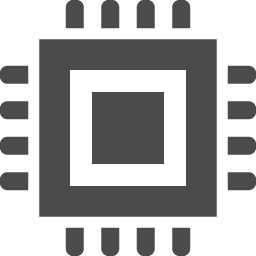
\includegraphics[height=7mm]{figs/assets/cpu.png}\\ syscall to native chip};
  \node[s, right=of s1] (s2) {cross-table lookup};
  \node[s, right=of s2] (s3) {trace $\to$ receipt (host-side cost)};
  \draw[->] (op) -- (e1); \draw[->] (e1) -- (e2); \draw[->] (e2) -- (e3);
  \draw[->] (op) -- (s1); \draw[->] (s1) -- (s2); \draw[->] (s2) -- (s3);
\end{tikzpicture}
\caption{The field-mismatch tax and what a precompile absorbs}
\label{fig:fmt-precompile}
\end{figure}
No existing SP1 chip computes a Griffin permutation over a $199$-bit prime field (Figure~\ref{fig:fmt-precompile} sketches the tax the missing chip leaves and what a precompile absorbs). The closest upstream pattern is SP1's Poseidon2 chip~\cite{succinct2024sp1}, implementing the Poseidon2 permutation~\cite{grassi2023poseidon2}, which has the same shape (a permutation precompile with single-pointer state I/O, per-round columns, and memory binding) but operates over SP1's $31$-bit base field (KoalaBear, $2^{31}-2^{24}+1$, in the evaluated fork). We therefore implement a custom AIR for one Griffin-$\pi$ permutation over $\mathbb{F}_p^{4}$, exposed to the guest as a single syscall on a state of $16$ $64$-bit words (four per lane, four lanes; each $256$-bit slot holding one $199$-bit element).

\paragraph{Per-round constraints.}
Each of the $14$ rounds is encoded by five per-round constraint families (the round-function families of Appendix~\ref{app:proofs}): a degree-$3$ forward S-box on one lane; an \emph{inverse} S-box on another lane, constrained in the backward direction ($y^d = x$ with the root witnessed) because the forward inverse exponent is a $199$-bit number that would blow past the constraint-degree budget; a quadratic layer on the remaining two lanes; the linear layer (the standard Griffin width-$4$ MDS matrix $M_4$, branch number $5$); and the SHAKE256-derived round constants. The backward constraint is valid because $\gcd(d,p-1)=1$ makes the cube map a bijection, so the witnessed root is unique. This side condition is \emph{not} automatic, and we verify it for the implemented modulus: with $d=3$ and $p = 2^{64}p_0+1$ we have $p-1 = 2^{64}p_0\equiv p_0\equiv 1\pmod 3$ (since $2^{64}\equiv 1\pmod 3$, and $p_0\equiv 1\pmod 3$ for the implemented $199$-bit modulus, verified by computation), hence $3\nmid(p-1)$ and $\gcd(3,p-1)=1$. Were $3\mid(p-1)$ the cube would be three-to-one and a malicious prover could witness a wrong root. The chip's remaining five families (round count, memory binding, output canonicality, row scheduling, parameter immutability) constrain the trace as a whole, as described next. The modulus, round count, linear-layer entries, round constants, and quadratic coefficients are bound in preprocessing rather than supplied per row, so a prover cannot choose them. A separate controller chip binds the syscall's memory reads and writes, and a per-lane output range check enforces output canonicality (\S\ref{ssec:bigint}'s cross-precompile contract). Two audit-driven hardening passes fixed a polynomial-degree blow-up and an all-zero-padding-row identity failure.

\subsection{The Sponge and Compression Wrapper}\label{ssec:sponge}
The chip exposes one permutation. Hashing needs a mode built around it. Algorithm~\ref{alg:guest-h2} gives the guest-side $2$-to-$1$ compression built on the syscall, and the construction follows.
% ---------- Algorithm 1: guest-side hashing path (Section 5.4) ----------
\begin{algorithm}[H]
\caption{Guest-side 2-to-1 compression $H_2$ via the
  \textsc{Griffin\_FP192\_Permute} syscall}
\label{alg:guest-h2}
\begin{algorithmic}[1]
\Require child digests $x=(x_0,x_1)\in\mathbb{F}_p^2$,
         $y=(y_0,y_1)\in\mathbb{F}_p^2$, canonical in $[0,p)$
\Ensure  digest $H_2(x,y)\in\mathbb{F}_p^2$
\State $s \gets (x_0, x_1, y_0, y_1)$
  \Comment{width $t_{\mathrm{state}}=4$, capacity $c_{\mathrm{cap}}=2$, rate $2$}
\State write $s$ to the state buffer in limb encoding
  \Comment{layout fixed by the syscall ABI; see \S\ref{ssec:griffin-air}}
\State \textbf{syscall} \textsc{Griffin\_FP192\_Permute}(\&$s$)
  \Comment{one cycle from the guest's perspective (\S\ref{sec:prelim})}
\State \Return $(s_0, s_1)$
  \Comment{truncate to the rate lanes}
\end{algorithmic}
\end{algorithm}

The permutation is wrapped in the sponge/compression construction of the Loquat instantiation to provide the $2$-to-$1$ compression used by PLUM's internal Merkle (BCS) commitments, the in-proof Griffin Merkle cost, and by the BDEC ledger trees the relying party checks outside the proof (Section~\ref{sec:prelim}). The state width is $t_{\mathsf{state}}=4$, the capacity $c_{\mathsf{cap}}=2$, and the rate $r=t_{\mathsf{state}}-c_{\mathsf{cap}}=2$, so a digest is the first two lanes of the output state. The $2$-to-$1$ compression of two child digests $x=(x_0,x_1)$ and $y=(y_0,y_1)\in\mathbb{F}_p^{2}$ is $H_2(x,y)=\big(\pi(x_0,x_1,y_0,y_1)\big)_{0,1}$, one application of the width-$4$ permutation $\pi$, truncated to the rate lanes. The SHAKE256 domain-separation seed and the linear-layer matrix are matched to the reference hasher, and cross-codebase tests pin the modulus, round count, linear-layer matrix, and seed against the reference implementation.

\subsection{Soundness of the Precompile Suite, and Two Open Questions}\label{ssec:soundness}
This subsection states the soundness claim and the two questions it leaves open. The per-constraint audit is deferred to Appendix~\ref{app:proofs}.

The theorem below is a functional (input--output) equivalence statement, and, conditional on the black-box-transfer hypothesis, a transfer of PLUM's EUF-CMA reduction. It is not a standalone cryptographic-security claim. The assumptions it names are stated formally in Section~\ref{sec:security}; each hypothesis carries its content here so the theorem is readable in place.

\begin{theorem}[Precompile soundness, conditional]\label{thm:precompile-sound}
Assume that
\begin{enumerate}
  \item the host zkVM's cross-table lookup argument is sound (Assumption~\ref{asm:lookup});
  \item the Griffin AIR's constraints are satisfied only by a witnessed transition equal to the reference Griffin-$\pi$ permutation (Assumption~\ref{asm:air});
  \item PLUM's EUF-CMA reduction treats Griffin and field multiplication as black-box input--output maps, inspecting no intermediate representation such as a limb of a field product (Assumption~\ref{asm:bbt}); and
  \item the upstream modular-multiplication guarantee of \S\ref{ssec:bigint} holds (Lemma~\ref{lem:fp192-mul}).
\end{enumerate}
Then substituting the precompile suite for the emulated operations preserves the input--output value of every PLUM and BDEC verification predicate, and, under the black-box-transfer hypothesis, PLUM's EUF-CMA reduction transfers unchanged. (The reduction's reliance on (Q)ROM-replaceability of this Griffin instantiation is a separate, upstream assumption, recorded as an open upstream assumption in Section~\ref{sec:security} and not discharged here.)
\end{theorem}

\begin{proof}[Proof sketch]
The input--output equality is Lemma~\ref{lem:relation-preserve} applied to each PLUM and BDEC verification predicate: under hypotheses (1), (2) and (4) the precompiles return the reference value of every large-field multiplication and Griffin permutation, so the accept-or-reject decision is unchanged. Granting Assumption~\ref{asm:bbt}, PLUM's EUF-CMA reduction is in the random-oracle model and depends only on the input--output behaviour of the hash function instantiating the oracle, which the precompile reproduces \emph{exactly} under Assumption~\ref{asm:air}; no random-oracle programming step in the reduction is affected, so it transfers unchanged.
\end{proof}

\paragraph{The precompile interface, and the family that instantiates it.}
Although stated for Griffin, the theorem's hypotheses are the \emph{interface} any precompile for an algebraic primitive in this family must meet: (i) input--output equivalence to the reference primitive over $\mathbb{F}_p$, so the chip computes the same function the emulated code did; (ii) isolation, so the outer proof sees only the syscall's committed inputs and outputs, never an intermediate limb (the black-box-transfer hypothesis together with lookup binding); and (iii) a constant, preprocessing-bound modulus, so a malicious prover cannot choose the field per row. To show that this interface is a reusable construction, we build \emph{three} instances of it over the same $199$-bit field, each meeting (i)--(iii) with a soundness argument of the same shape: the Griffin permutation AIR (\S\ref{ssec:griffin-air}); a dedicated \texttt{FP192\_MUL} field-multiplication chip; and a \texttt{FP192\_POW\_RES} chip that composes the field multiplication into the power-residue-PRF symbol check $a^{(p-1)/t}\bmod p$ under a fixed square-and-multiply schedule, the steps bound row-to-row by a cross-table lookup. All three build and pass a core-STARK smoke proof (execute, prove, verify), and \texttt{FP192\_POW\_RES} additionally completes the multi-symbol (multi-shard) prove a real power-residue batch requires, after correcting an executor timestamp that had desynchronised its memory records across a shard boundary. Its row-to-row chain binding was also checked against an adversarial soundness review, and its user/\texttt{mprotect} path is disabled (it carries no page-protection columns), so it is validated at the same core-prove level as Griffin but not for an untrusted user path.

\emph{Measured versus demonstrated.} Only the Griffin AIR is on the measured path. The measured PLUM-verify figure of Section~\ref{sec:evaluation} is produced by the Griffin chip together with the host \texttt{UINT256\_MUL} for field multiplication, not by the \texttt{FP192\_MUL} or \texttt{FP192\_POW\_RES} chips. Those two are built to demonstrate that the interface \emph{generalises} across primitive classes (a permutation, a field multiplication, and a composed modular exponentiation) and they also locate where the criterion's \emph{positive} question lives. \texttt{FP192\_MUL} re-implements arithmetic the host \texttt{UINT256\_MUL} precompile already serves (it is essentially that host chip retargeted), so the criterion predicts it does not pay. The chips' committed dimensions sharpen rather than simply confirm this. The dedicated chip is in fact ${\approx}18\%$ \emph{narrower} per operation ($304$ versus $371$ committed cells, since hardcoding the modulus deletes the modulus-from-memory columns the host chip carries; \rr{docs/measurements/keystone_chipprove_20260706}). So on per-operation area alone it leans toward paying. The predicted not-pay verdict rests instead on the fixed whole-table overhead a dedicated chip adds to the recursion and verify shapes (the fixed layouts provisioned for the wrap's recursion stages; Section~\ref{sec:evaluation}), the same cost this thesis documents for Griffin. An $18\%$ per-operation saving over an already-present host chip does not amortise that overhead. That whole-machine cost we do not measure end-to-end, so this verdict is a design-level prediction of the criterion, not a measured outcome. \texttt{FP192\_POW\_RES} is the component whose pay-or-not verdict is not settled by per-operation area alone. The power-residue symbol $a^{(p-1)/t}\bmod p$ is the one verifier component that is \emph{irreducibly large-prime} for two independent reasons. Its PRF security is $O(\sqrt p)$ key recovery (established for the Legendre ($t{=}2$) case~\cite{khovratovich2019legendre,may2022legendre}, on whose hardness the general $t$-th residue rests), so the prime cannot shrink to a matched field the way the hash can (the SHA-3 control of Section~\ref{sec:evaluation} shows the hash can); and the STIR low-degree test needs a smooth multiplicative subgroup of the same $\mathbb{F}_p$~\cite{cryptoeprint:2024/390}. Either bind makes it the natural target for a bespoke chip. Whether that chip \emph{pays} turns on a control-overhead saving that a per-operation comparison hides. Per symbol the naive dedicated chip commits more field-operation area than the guest loop, evaluating both square-and-multiply branches unconditionally, so on the per-operation arithmetic axis alone it does not pay; but that axis omits the per-symbol control overhead of the square-and-multiply schedule the chip replaces (one syscall dispatch, memory access, and lookup for each of the ${\approx}261$ multiplications, against one for the chip). The deciding trace-area experiment, isolating exactly that saving (the chip against the guest loop on \emph{total} committed area, field-operation plus control, at the honest baseline), is specified here and run in Section~\ref{sec:evaluation} (\S\ref{sssec:already-served}), where the criterion's positive case is decided. Griffin, by contrast, is field-mismatched \emph{and} unserved, the configuration in which the criterion expects a precompile to pay. Its verdicts under both baselines are likewise Section~\ref{sec:evaluation}'s. The shared interface is what lets the three chips serve as evidence for one method rather than three separate constructions.

\paragraph{What is established.}
The field-substrate half rests on the reduction of \S\ref{ssec:bigint}. The suite includes the bespoke Griffin AIR, to which Assumption~\ref{asm:air} applies. For the Griffin AIR, the per-family analysis (Appendix~\ref{app:proofs}) exhibits, family by family, the constraint \emph{intended} to catch any deviation from reference Griffin, the forgery that deviation would enable, and the implementation status of each. Memory binding, output canonicality, parameter immutability, and row scheduling are implemented and constrained. What that analysis does \emph{not} establish, and says so explicitly, is that the implemented constraint system is satisfied \emph{only} by reference-equal witnesses. Assumption~\ref{asm:air} names it the \emph{chip--constraint equality}. It is empirically supported by the $256$-vector cross-codebase agreement and the partial fault-injection coverage discussed below (per-vector false-pass probability $\approx 2^{-199}$ for the vector suite), but the vector agreement pins the \emph{executor} against the reference, a weaker \emph{chip--executor} equality, not the \emph{constraints}. Assumption~\ref{asm:air} is not verified at the constraint level.

\paragraph{Open question 1: Assumption~\ref{asm:air} is empirically supported but unproved.}
The $256$-vector agreement establishes that the executor's native compute equals the reference permutation. It does \emph{not} by itself establish that the \emph{AIR constraints} admit only that computation. For the per-row layer (the per-row families) that stronger statement carries a written proof. Appendix~\ref{app:proofs} bridges the limb identities the chip constrains over its small base field to congruences modulo $p$ and composes them into the reference round, conditional only on the byte-range lookups that the lookup-binding hypothesis already covers. A separate fault-injection suite corroborates this layer in the rejection direction via \texttt{debug\_constraints}. Single-cell corruptions of a satisfying trace are rejected for each of the seven per-row families. The three lookup-borne families (round count, memory binding, and the cross-row threading of row scheduling) lie outside \texttt{debug\_constraints}, which does not evaluate cross-table lookups; we reach them with a separate lookup-balance harness (\texttt{debug\_interactions}) that computes the net multiplicity ($\sum$ sends $-\sum$ receives) of the Griffin cross-table lookup, a nonzero value being an imbalance the verifier rejects, conditional on the lookup-binding assumption. A short round chain (round count) and a broken cross-row state thread (row scheduling) each produce the predicted imbalance and are rejected; memory binding is rejected for the syscall-level state handoff at the committed clock and pointer, while its global-memory-consistency half, that the controller's read equals historical guest memory, is a lookup to the global memory chip that needs the full machine and is not covered. Parameter immutability is argued by construction. What Assumption~\ref{asm:air} still carries splits in two, and each needs a different tool. The code-to-constraint transcription fidelity of the per-row layer, that the constraints admit only the honest witness, would be closed by deriving the AIR witness from the same reference code and checking full-row constraint satisfaction directly, ideally by machine. The three lookup-borne families lie outside that per-row check, their cross-table binding not being a per-row property; the lookup-balance harness above exercises them in the rejection direction (round count and cross-row threading fully, memory binding for the syscall handoff), leaving the global-memory-consistency lookup uncovered and, for all three, the no-wrong-witness direction open and conditional on the lookup-binding assumption.

\paragraph{Open question 2: the classical security floor at our parameters and the QROM lift are upstream of the AIR.}
PLUM's EUF-CMA argument under Fiat--Shamir requires Griffin to be replaceable by a (quantum) random oracle. The Griffin analyses cover the original instantiations. Whether they cover this $d=3$, width-$4$, $199$-bit-field, $14$-round instantiation is not something the AIR can settle. If this instantiation were QROM-distinguishable, no amount of AIR engineering would recover security. We have surveyed the classical Griffin algebraic-attack frontier and placed this instance against the broken ones (Section~\ref{sec:security}, Table~\ref{tab:round-margin}), and it is not among them. What that survey leaves open, and what we do not close here, is two things. The classical security floor at our exact parameters still needs the FreeLunch and Improved-Resultant estimator instantiated at $(r{=}14,d{=}3,t_{\mathsf{state}}{=}4,\log_2 p\approx199)$, and the QROM lift, whether this instantiation is quantum-random-oracle-indistinguishable and whether PLUM's Fiat--Shamir reduction lifts to the quantum random-oracle model, is upstream of the AIR.

\paragraph{Further limitations.}
The EUF-CMA reduction is argued to transfer on the grounds that the reference reduction treats Griffin and field multiplication as black-box input--output maps, but we have not audited PLUM's reduction line by line for a step that inspects an \emph{intermediate} representation (such as a limb of a field product), which input--output equality alone would not cover. The zero-knowledge property required by BDEC's anonymity guarantee is a property of the proof wrap, analysed as the anonymity--deployability tension of Section~\ref{sec:security} and measured in Section~\ref{sec:evaluation}, not closed here.

\subsection{Integration into the Credential Relations (BDEC Instance)}\label{ssec:integration}
The credential-generation relation $R_{\mathsf{cre}}^{\Sig}$ of Section~\ref{sec:prelim}, instantiated with PLUM as $\Sig$, is the AND concatenation of two PLUM signature verifications, both under the user's public key $\pk_U$, with public statement $x_{\mathsf{cre}}=(c_{U,TA},h_{U,TA},\mathsf{ppk}_{U,TA})$ and witness $w_{\mathsf{cre}}=(\pk_U,\mathsf{psk}_{U,TA})$. We implement this relation \emph{in full} as an SP1 guest, with PLUM in place of Loquat and field multiplications routed through \texttt{UINT256\_MUL}. The guest computes exactly the two $\Pred_{\Verify}$ conjuncts that define base CreGen, with no omitted predicate. (The optional Merkle-accumulator variant of Remark~\ref{rem:merkle-extension} is not part of this relation and performs its membership checks in $\BDEC.\mathsf{ShowVer}$. It is out of scope here.) The guest binds the proof to its public statement: it commits $x_{\mathsf{cre}}=(c_{U,TA},h_{U,TA},\mathsf{ppk}_{U,TA})$ to the proof's public values, so an accepting receipt certifies \emph{which} statement was proved rather than merely ``two signatures verify under some witness''. This binding bears on security and is not a cosmetic completeness gap; it is discharged here and measured in Section~\ref{sec:evaluation}, at essentially the cost of the outcome-only prove since the commitment is a few field elements and does not alter the proved relation. The public parameters, $\pk_U$, and both messages enter the guest as private inputs, and $h_{U,TA}$ and the pseudonym are formed on the host and passed in as opaque messages. Committing $x_{\mathsf{cre}}$ binds the receipt to that specific $h_{U,TA}$. A fully attribute-bound verifier that also proved $h_{U,TA}=H(A)$ in-circuit would recompute these hashes there, a further step this relation does not take. In execute mode at $\lambda=80$ the guest runs both verifications to acceptance, the two costing essentially the same, confirming that both pass through the same precompile-backed path (guest-cycle counts in Section~\ref{sec:evaluation}). The transition from this execute-mode validation to a completed proof is the subject of Section~\ref{sec:evaluation}. Both relations complete a succinct (non-zero-knowledge) prove on SP1, a receipt distinct from the zero-knowledge wrap. The prove times and the CreGen shard-configuration provenance are reported in Section~\ref{sec:evaluation}.

The full presentation relation (ShowCre), the $k+2$-verification generalisation of this relation, is likewise implemented as an SP1 guest, validated in execute mode at $k=1,2$ and, like CreGen, statement-bound in prove mode by an end-to-end run committing $x_{\mathsf{show}}$ at $k=2$ (Section~\ref{sec:evaluation}). Its zero-knowledge wrap also completes and verifies on the target hardware at both $k=1$ and $k=2$ (the latter statement-bound), each within the memory budget, with the full timing, peak memory, and provenance in Section~\ref{sec:evaluation}.

    \newpage
    \section{Security Analysis}\label{sec:security}
This section answers one question. Which of the credential's security properties survive the move to the zkVM substrate? The answer, established below, has three parts. Knowledge soundness (that only someone who genuinely holds a valid signature can produce an accepting proof) transfers, under Assumptions~\ref{asm:air} and~\ref{asm:lookup} and Conjecture~\ref{conj:extract-recursion}. Classical zero-knowledge is delivered within the memory budget, by the pairing wrap. Deployable post-quantum anonymity is not delivered on this stack.

Section~\ref{sec:system} described the precompile suite, which moves PLUM's dominant field operations out of emulated guest code. A performance change to a credential system is meaningful only if it does not silently weaken the security the system provides. This section makes that requirement precise. We fix the security model and threat model in Section~\ref{ssec:threat-model}, prove in Section~\ref{ssec:preservation} a preservation theorem that bounds how far the move to a zkVM substrate and the precompile suite can shift the adversary's advantage in each of BDEC's security experiments, and then isolate in Section~\ref{ssec:zk-gap} the one property the analysis does not deliver on consumer hardware, namely \emph{post-quantum} anonymity of the proof actually produced. The preservation theorem is conditional, and it rests on two essential premises, which we name here. The first is Assumption~\ref{asm:air}, the constraint-level chip-equivalence of the Griffin-$\mathbb{F}_p^{192}$ AIR, namely that its constraint system is satisfied only by a witnessed transition equal to the reference permutation. The second, for the knowledge soundness of the composite multi-shard receipt the prover actually emits, is the extractor conjecture stated with the analysis (Conjecture~\ref{conj:extract-recursion}), which is stated, not proved. The former premise is empirically supported, by a $256$-vector cross-codebase equivalence suite and rejection-direction fault injection on seven of its ten constraint families, and it is not yet verified at the constraint level for the three lookup-borne families; We carry each premise as a scoped open condition, not a defect. Closing the first is machine-checking rather than new theory. Closing the second is a composition proof. The anonymity finding, in turn, is not a weakness in the construction. A classically-secure zero-knowledge wrap of the receipt completes within the consumer memory budget (Section~\ref{ssec:zk-gap}), so the obstruction is not that the anonymity-providing proof fails to run but that the only wrap the toolchain exposes is pairing-based, hence classically secure only. Given that the precompile suite is what lets PLUM verification run inside the zkVM at all (Section~\ref{sec:system}), this section fixes \emph{which} of the credential's security properties survive that move and which it leaves out of reach, the three-part answer stated at the outset. What the move costs is priced separately by the cost criterion of Sections~\ref{sec:theoretical} and~\ref{sec:evaluation}.

\subsection{Security Model and Threat Model}\label{ssec:threat-model}
BDEC is proved secure in three experiments, formalised in Section~\ref{sec:prelim}. Unforgeability requires that an adversary with issuance and showing oracles cannot produce an accepting showing for a statement outside its honestly issued set, beyond negligible advantage. Anonymity and unlinkability are challenge-bit experiments in which the adversary cannot distinguish, beyond advantage $|\Pr[b'=b]-\tfrac12|$, which of two honestly issued credentials produced a challenge showing (anonymity) or under which of two pseudonyms a single challenge credential was issued (unlinkability). We write $\mathsf{Adv}^{\mathsf{unf}}_{\AC}$, $\mathsf{Adv}^{\mathsf{anon}}_{\AC}$, and $\mathsf{Adv}^{\mathsf{unlink}}_{\AC}$ for the respective advantages, all defined in Section~\ref{sec:prelim}.
\begin{definition}[zkVM credential advantage]\label{def:zkvm-cred-adv}
    For $\bullet\in\{\mathsf{unf},\mathsf{anon},\mathsf{unlink}\}$, write $\mathsf{Adv}^{\bullet}_{\mathsf{zkVM\text{-}Cred}}(\mathcal A)$ for the advantage $\mathsf{Adv}^{\bullet}_{\AC}(\mathcal A)$ of Section~\ref{sec:prelim} evaluated on the BDEC scheme instantiated with PLUM as the signature scheme $\Sig$ and the zkVM as the zkSNARK $\Pi$.
\end{definition}

Unfolding Definition~\ref{def:zkvm-cred-adv}, the experiments defining $\mathsf{Adv}^{\bullet}_{\mathsf{zkVM\text{-}Cred}}$ for $\bullet\in\{\mathsf{unf},\mathsf{anon},\mathsf{unlink}\}$ are as follows. We first fix the proved object and the zkVM interface, then the oracles, then the three games. Each game restates the corresponding Section~\ref{sec:prelim} experiment with the standard adaptive oracle interface and the zkVM receipt interface, the $\mathsf{JBind}$ conjunct being the receipt-model translation of ``$\pi$ verifies against $x$'' rather than a change of the win predicate, evaluated on BDEC instantiated with PLUM and the zkVM, so BDEC's Theorems~1--3 bounds still apply. For orientation: each assumption below is stated formally, most with a named error term (the knowledge-soundness and simulator games of Definitions~\ref{def:ks} and~\ref{def:szk} and the zero-knowledge game of Definition~\ref{def:zk}, all stated formally in Appendix~\ref{app:prsv-defs}, and the arithmetisation-soundness defect $\epsilon_{\mathrm{AIR}}$ of Assumption~\ref{asm:air}; a few, such as the black-box-transfer property, are binary and carry none). The assembled advantage is the expanded per-experiment sum of Equations~\eqref{eq:adv-unf} and~\eqref{eq:adv-anon} together with the unlinkability specialisation and the separate issuance-anonymity bound, over six leaf error terms (the five named in Theorem~\ref{thm:security-preserve} plus $\epsilon_{\mathrm{keypriv}}$ for issuance) with the tightness factors given there. These \emph{error terms} are a different list from the five open \emph{assumptions} named below. An assumption does not always carry an error term. The \emph{status} of each, established, assumed, or open, is set out term by term after the theorem.

\paragraph{A zero-knowledge proof of knowledge of a valid signature.}
The object the credential prover produces is not a signature verification but a \emph{zero-knowledge argument of knowledge} of a witness that makes a signature-verification relation accept, with that witness hidden. Checking a signature is easy once the signature is in hand. The difficulty this thesis instruments is to certify that such a signature exists \emph{without revealing it, or the key it verifies under}. Fix $\ppSig\leftarrow\Sig.\Setup(1^\lambda)$ and recall the efficiently decidable credential relation of Section~\ref{sec:prelim}. Every value to be signed is first mapped into the message space by $\EncodeSig:\{0,1\}^{\ast}\to\MSig$, so $h_{U,TA}=H(A)\in\MSig$ and the pseudonym is signed under the encoded message $m_{\mathsf{nym}}:=\EncodeSig(\mathsf{ppk}_{U,TA})$; the signatures are produced honestly by $c_{U,TA}\leftarrow\Sig.\Sign(\ppSig,\sk_U,h_{U,TA})$ and $\mathsf{psk}_{U,TA}\leftarrow\Sig.\Sign(\ppSig,\sk_U,m_{\mathsf{nym}})$. With this encoding the credential relation reads
\begin{equation*}
  R_{\mathsf{cre}}^{\Sig}(x_{\mathsf{cre}};w_{\mathsf{cre}})=1
  \Longleftrightarrow
  \Pred_{\Verify}^{\Sig,\ppSig}(\pk_U,h_{U,TA},c_{U,TA})=1
  \ \land\
  \Pred_{\Verify}^{\Sig,\ppSig}(\pk_U,m_{\mathsf{nym}},\mathsf{psk}_{U,TA})=1,
\end{equation*}
with public instance $x_{\mathsf{cre}}=(c_{U,TA},h_{U,TA},\mathsf{ppk}_{U,TA})$ and \emph{private} witness $w_{\mathsf{cre}}=(\pk_U,\mathsf{psk}_{U,TA})$. Membership is decidable in time polynomial in $|x_{\mathsf{cre}}|+|w_{\mathsf{cre}}|$ by running $\Sig.\Verify$ twice. The credential prover supplies a proof $\pi$ for ``$\exists\,w_{\mathsf{cre}}:R_{\mathsf{cre}}^{\Sig}(x_{\mathsf{cre}};w_{\mathsf{cre}})=1$'' that is zero-knowledge in $w_{\mathsf{cre}}$. $\pk_U$, though public \emph{by type}, is used here as a hidden witness \emph{by role}. Revealing it would tie the showing to the user's identity, so anonymity requires $\pk_U\in w_{\mathsf{cre}}$, never in $x_{\mathsf{cre}}$. The same reading carries to the showing relation $R_{\mathsf{show}}^{\Sig}$ with its $k+2$ predicate conjuncts, where each pseudonym message is $m_{\mathsf{nym}}^{(j)}:=\EncodeSig(\mathsf{ppk}_{U,TA}^{(j)})$ as in Section~\ref{sec:prelim}.

\paragraph{Modelling the zkVM interface and journal-binding inside the game.}
The proof is produced by a zkVM whose universal relation is $R_{\mathsf{vm}}\bigl((\mathsf{img},\mathsf{in}_{\mathsf{pub}},\mathsf{out});(\mathsf{P},\mathsf{in}_{\mathsf{priv}})\bigr)=1$ iff $\mathsf{img}=\mathsf{digest}(\mathsf{P})$ and running guest $\mathsf{P}$ on $(\mathsf{in}_{\mathsf{pub}},\mathsf{in}_{\mathsf{priv}})$ terminates emitting public output $\mathsf{out}$; the public instance is $x_{\mathsf{vm}}=(\mathsf{img},\mathsf{in}_{\mathsf{pub}},\mathsf{out})$ and the witness $w_{\mathsf{vm}}=(\mathsf{P},\mathsf{in}_{\mathsf{priv}})$. The host supplies inputs over a \emph{read} channel and receives outputs over a \emph{commit} channel. Values placed on the commit channel enter $\mathsf{out}$ and become public, values read but not committed stay in $\mathsf{in}_{\mathsf{priv}}$ and remain hidden. In the BDEC instantiation $\sk_U$, $\pk_U$, and the credential signatures enter only via the read channel and are never committed, so they remain in $w_{\mathsf{vm}}$ across the entire relation, which is what keeps $w_{\mathsf{cre}}$ hidden. We make the binding of the public statement an explicit predicate of the game:
\begin{equation*}
  \mathsf{JBind}(\mathsf{out},x)=1
  \iff
  \text{$x$ is committed on the commit channel, i.e.\ $x$ is recoverable from $\mathsf{out}$.}
  % \mathsf{JBind}: journal-binding indicator, written inline; no macro introduced.
\end{equation*}
An accepting receipt certifies only ``$\exists\,w:R(x;w)=1$ for the $x$ that $\mathsf{JBind}$ pins down''. The games below carry $\mathsf{JBind}$ as an explicit conjunct in the win condition, so that they model the committed system in which $x_{\mathsf{cre}}$ is committed to the journal, which both credential relations now implement (Section~\ref{sec:evaluation}); the earlier boolean-only variant, which removes it, we state explicitly after the games.

\paragraph{The wrap's public instance, and what it leaks.}
Instantiated on the deployed stack, the public instance $x_{\mathsf{vm}}=(\mathsf{img},\mathsf{in}_{\mathsf{pub}},\mathsf{out})$ carries only two statement-bearing components, the read-channel inputs being private so that $\mathsf{in}_{\mathsf{pub}}$ is empty: $\mathsf{img}$, a commitment to \emph{which} guest program was proved, and $\mathsf{out}$, a digest whose preimage is exactly the statement $x$---$x_{\mathsf{cre}}=(c_{U,TA},h_{U,TA},\mathsf{ppk}_{U,TA})$ for issuance, $x_{\mathsf{show}}=((\mathsf{ppk}_{U,TA}^{(j)})_{j=1}^{k},\mathsf{ppk}_{U,V},h_{U,V})$ for showing---together with the aggregate accept bit. Here $h_{U,V}:=H(A^\downarrow)$ is the disclosed-attribute digest, the showing analogue of $h_{U,TA}=H(A)$: the receipt commits this constant-size digest in place of $A^\downarrow$ itself, which the verifier still checks in the clear (\S\ref{sec:prelim}), so the committed showing statement and the anonymity game's canonical $x_{\mathsf{show}}=(A^\downarrow,(\mathsf{ppk}_{U,TA}^{(j)})_{j=1}^{k},\mathsf{ppk}_{U,V})$ name the same disclosure, $h_{U,V}$ being a deterministic function of the disclosed $A^\downarrow$.\footnote{The concrete SP1 wrap proof additionally publishes three witness-independent constants, a guest halt code, a verifying-key-set root, and a prover nonce, that depend on no part of $w_{\mathsf{vm}}$ and carry no user information.} The wrapped proof \emph{leaks nothing beyond $x_{\mathsf{vm}}$}, which resolves into two obligations. First, the wrap is zero-knowledge: by Definition~\ref{def:zk} it hides $w_{\mathsf{vm}}$, and with it $\pk_U$, the signatures, and the entire execution trace, though only against a classical distinguisher, the wrap being pairing-based over {BN254} (the second obstruction, \S\ref{ssec:zk-gap}). Second, $\mathsf{out}$ commits only the intended disclosures $\mathsf{Leak}(x)$ and no witness residue, since $\pk_U$, $\mathsf{psk}_{U,TA}$, and every signature travel the read channel alone. Zero knowledge hides the witness. It does not hide what the public statement itself reveals. What the wrap therefore delivers is \emph{pseudonymity}, the real identity $\pk_U$ staying hidden, together with unlinkability on the freshly sampled verifier-facing pseudonym $\mathsf{ppk}_{U,V}$, scoped by the equal-$\mathsf{Leak}$ admissibility of the anonymity game below; it is not concealment of the teaching-authority pseudonym $\mathsf{ppk}_{U,TA}$, a public ledger handle by design (\S\ref{sec:prelim}).

\paragraph{Oracles.}
All three experiments give the challenger an honest-user registry populated at setup (so that the notion of an honestly generated user key pair is well defined, exactly as in Section~\ref{sec:prelim}) and an issuance log $\mathcal L$ of tuples $(\mathsf{ipk},\mathsf{upk},A,\mathsf{cred})$, together with the following two oracles, to which the adversary $\Adv$ has \emph{adaptive} access. There is no corruption oracle. The source model of Section~\ref{sec:prelim} exposes only issuance and showing, and the cited BDEC bounds are proved against exactly this interface.
\begin{itemize}
    \item $\mathcal O_{\mathsf{Issue}}(i,A)$: for a registered honest user $i$, runs the honest issuance path. The teaching authority signs
    \begin{equation*}\sigma_{\mathsf{cred}}\leftarrow\Sig.\Sign(\ppSig,\sk_{TA},\EncodeSig(\pk_U,\mathsf{ppk}_{U,TA},A,\mathsf{aux})),\end{equation*}
    the ledger stores the record digest $\rho_{U,TA}=H(\pk_{TA},\mathsf{ppk}_{U,TA},A,\mathsf{aux},\sigma_{\mathsf{cred}})$, the challenger appends $(\mathsf{ipk},\mathsf{upk},A,\mathsf{cred})$ to $\mathcal L$, and returns the issued credential material.
    \item $\mathcal O_{\mathsf{Show}}(i,\phi,A^\downarrow)$: for a registered honest user $i$, runs honest $\BDEC.\mathsf{ShowCre}$ and returns the receipt $(x_{\mathsf{vm}},\mathsf{receipt})$, i.e.\ the public statement $x_{\mathsf{show}}=(A^\downarrow,(\mathsf{ppk}_{U,TA}^{(j)})_{j=1}^{k},\mathsf{ppk}_{U,V})$ and the proof $\pi$; the presentation predicate $\phi$ is adversary-chosen at show time.
\end{itemize}

\begin{gamebox}{Experiment $\mathsf{Exp}^{\mathsf{unf}}_{\mathsf{zkVM\text{-}Cred},\Adv}(\lambda)$ (unforgeability)}
    \emph{Model: classical PPT adversary, classical random-oracle model.}\par\smallskip
    \begin{enumerate}
        \item The challenger samples $\parms=(\ppSig,\crs,\mathsf{img})\leftarrow\BDEC.\Setup(1^\lambda)$, where $\mathsf{img}$ is the fixed guest-image digest of the credential guest, initialises $\mathcal L\gets\emptyset$ and the honest-user registry, and gives $\parms$ and the public ledger roots $(\mathsf{rt}_{\mathsf{cred},e},\mathsf{rt}_{TA,e},\mathsf{rt}_{\RL,e})$ to $\Adv$.
        \item $\Adv$ interacts adaptively with $\mathcal O_{\mathsf{Issue}}$ and $\mathcal O_{\mathsf{Show}}$.
        \item $\Adv$ outputs $(\mathsf{ipk}^\star,x^\star,\mathsf{receipt}^\star)$ with $\mathsf{receipt}^\star=(\mathsf{out}^\star,\pi^\star)$ and public instance $x_{\mathsf{vm}}^\star=(\mathsf{img},\mathsf{in}_{\mathsf{pub}}^\star,\mathsf{out}^\star)$, where $\mathsf{in}_{\mathsf{pub}}^\star$ is empty, as the deployed instance fixes (the wrap-instance paragraph above).
        \item The experiment outputs $1$ iff
        \begin{equation*}
          \Pi_{\mathsf{vm}}.\Verify(\crs, x_{\mathsf{vm}}^\star, \pi^\star)=1
          \ \land\
          \mathsf{JBind}(\mathsf{out}^\star,x^\star)=1,
        \end{equation*}
        and the relying party's verifier-side checks of Section~\ref{sec:prelim} accept: $\mathsf{ipk}^\star$ is an authorised teaching authority (a member under the published root $\mathsf{rt}_{TA,e}$) and the statement's teaching-authority pseudonym(s), $\mathsf{ppk}_{U,TA}$ for issuance and $(\mathsf{ppk}_{U,TA}^{(j)})_j$ for a showing, are \emph{anchored}, each appearing in an accepted ledger record under $\mathsf{rt}_{\mathsf{cred},e}$ (the ledger the challenger maintains, so an anchored pseudonym was issued through $\mathcal O_{\mathsf{Issue}}$ and its record binds a registered honest key; the freshly sampled verifier-facing pseudonym $\mathsf{ppk}_{U,V}$ is not a ledger object and carries no anchoring requirement); and the forgery is \emph{fresh}, in the win predicate of Section~\ref{sec:prelim}: no honestly produced material explains the statement, i.e.\ there is no witness under a registered honest user key, assembled from the challenger's honestly issued credentials (the tuples of $\mathcal L$) and honestly produced showing-time signatures (the $\mathcal O_{\mathsf{Show}}$ material), that satisfies the relation on $x^\star$. This in particular excludes a verbatim replay of an $\mathcal O_{\mathsf{Show}}$ receipt and a re-proof of its statement. We abbreviate this freshness clause $x^\star\notin\mathcal L$.
    \end{enumerate}
    $\displaystyle
    \mathsf{Adv}^{\mathsf{unf}}_{\mathsf{zkVM\text{-}Cred}}(\Adv)=\Pr\!\bigl[\mathsf{Exp}^{\mathsf{unf}}_{\mathsf{zkVM\text{-}Cred},\Adv}(\lambda)=1\bigr].$ The experiment itself runs no extractor: knowledge soundness ($\epsilon_{\mathrm{KS}}$) is spent by the reduction (Appendix~\ref{app:preservation}), whose first hop extracts a witness from the accepting receipt. The $\mathsf{JBind}$ conjunct pins the committed statement $x^\star$ that the extracted witness must satisfy, and the anchoring conjunct ties the forgery to the challenger's registry, which the reduction's honest-key guess requires.
\end{gamebox}

\begin{gamebox}{Experiment $\mathsf{Exp}^{\mathsf{anon}}_{\mathsf{zkVM\text{-}Cred},\Adv}(\lambda)$ (anonymity)}
    \emph{Model: classical PPT adversary, classical random-oracle model.}\par\smallskip
    \begin{enumerate}
        \item Setup as above; $\Adv$ receives $\parms$, the roots, and adaptive access to $\mathcal O_{\mathsf{Issue}}$ and $\mathcal O_{\mathsf{Show}}$.
        \item $\Adv$ designates two entries of the issuance log $\mathcal L$, honestly issued credentials $(\mathsf{cred}_0,A_0)$ and $(\mathsf{cred}_1,A_1)$ of registered honest users whose secret keys $\mathsf{usk}_0,\mathsf{usk}_1$ remain with the challenger (there being no corruption oracle), together with a predicate $\phi$ with $\phi(A_0)=\phi(A_1)=1$ and disclosed attributes $A^\downarrow$.
        \item Well-formedness: the challenge is admissible only if $\mathsf{Leak}(x_0)=\mathsf{Leak}(x_1)$, where $\mathsf{Leak}(\cdot)$ projects the statement onto its intentionally-disclosed components, namely $A^\downarrow$, the teaching-authority pseudonym multiset $\{\mathsf{ppk}_{U,TA}^{(j)}\}$ (carried in the statement in the holder's canonical record order, so multiset equality equalises the ordered component), and any linking tag carried in $\phi$; the verifier-facing pseudonym $\mathsf{ppk}_{U,V}$ is freshly sampled at showing time.
        \item The challenger samples $b\leftarrow\{0,1\}$ and returns $(x,\mathsf{receipt}_b)\leftarrow\BDEC.\mathsf{ShowCre}$ for $\mathsf{cred}_b$, run with the designated user's witness material, which the challenger holds.
        \item $\Adv$, with continued oracle access, outputs $b'$.
    \end{enumerate}
    $\displaystyle
    \mathsf{Adv}^{\mathsf{anon}}_{\mathsf{zkVM\text{-}Cred}}(\Adv)=\Bigl|\Pr[b'=b]-\tfrac12\Bigr|.$ The bound established below for this advantage is made effective only when the receipt is zero-knowledge in $w_{\mathsf{vm}}$; on the shipped succinct-STARK path it is not (Section~\ref{ssec:zk-gap}), so it is sound but not effective there. Non-cryptographic side channels (timing, ledger-access and revocation-update patterns, wallet metadata) are outside this model.
\end{gamebox}

\begin{gamebox}{Experiment $\mathsf{Exp}^{\mathsf{unlink}}_{\mathsf{zkVM\text{-}Cred},\Adv}(\lambda)$ (unlinkability)}
    \emph{Model: classical PPT adversary, classical random-oracle model.}\par\smallskip
    \begin{enumerate}
        \item Setup and the \emph{same} oracle interface as the unforgeability experiment ($\mathcal O_{\mathsf{Issue}}$ and $\mathcal O_{\mathsf{Show}}$), available adaptively to $\Adv$.
        \item The challenger registers an honest user $(\sk_U,\pk_U)$ and creates two pseudonyms $\mathsf{ppk}^0,\mathsf{ppk}^1$, freshly and identically sampled, each bound to the user's key by its binding signature $\mathsf{psk}^i\leftarrow\Sig.\Sign(\ppSig,\sk_U,\EncodeSig(\mathsf{ppk}^i))$ (Section~\ref{sec:prelim}). The pseudonyms are internal to the challenger and are \emph{not} given to $\Adv$, whose only view of them is through the challenge receipt below. The challenger creates an attribute set $A^\downarrow$, samples $b\leftarrow\{0,1\}$, and issues a \emph{single} credential $c^{(b)}$ with respect to $\mathsf{ppk}^{(b)}$ on $A^\downarrow$.
        \item The challenger runs $\mathsf{ShowCre}$ on $c^{(b)}$ under a freshly-sampled verifier-facing pseudonym $\mathsf{ppk}_{U,V}$, holding the credential $c^{(b)}$ as a private witness, and forwards the resulting zero-knowledge showing receipt (with public statement $x_{\mathsf{show}}$, not the raw credential) to $\Adv$.
        \item $\Adv$ outputs $b'$.
    \end{enumerate}
    $\displaystyle
    \mathsf{Adv}^{\mathsf{unlink}}_{\mathsf{zkVM\text{-}Cred}}(\Adv)=\Bigl|\Pr[b'=b]-\tfrac12\Bigr|.$ When the statements intentionally carry a public linking tag, linkability is allowed only as that tag determines. The single-transcript structure is why the one-transcript simulation applies once, giving unlinkability the single-transcript ($k{+}2\to1$) specialisation of the anonymity bound.
\end{gamebox}

\paragraph{The shipped-prototype game.}
Both credential relations commit their public statement, so $\mathsf{JBind}=1$ (Section~\ref{sec:evaluation}). Where a guest commits only the verification outcome, a single boolean, $\mathsf{JBind}(\mathsf{out}^\star,x^\star)=0$ for every nontrivial $x^\star$; modelling that case means deleting the $\mathsf{JBind}$ conjunct from the unforgeability win condition above. With that conjunct gone the extracted $x^\star$ is unpinned, and the adversary trivially satisfies statement-binding with any $x^\star$ consistent with the one committed boolean, so an accepting receipt attests merely ``two signatures verify under \emph{some} witness''. Such a receipt is a functional benchmark, not a statement-bound verifier; committing the public statement to the journal, as both credential relations now do, restores the conjunct and closes the gap.

\begin{assumption}[Griffin-AIR constraint soundness]\label{asm:air}
    The Griffin-$\mathbb{F}_p^{192}$ AIR admits only the reference permutation: its constraint system is satisfied solely by a witnessed transition equal to reference Griffin-$\pi$, equivalently the arithmetisation soundness defect $\epsilon_{\mathrm{AIR}}$ of Definition~\ref{def:eair} is zero. This assumption is \emph{open}. It is argued at the specification level in Appendix~\ref{app:proofs} and empirically supported by the $256$-vector cross-codebase equivalence suite together with rejection-direction fault injection on the seven per-row families (via \texttt{debug\_constraints}) and, via a lookup-balance harness, the three lookup-borne families (memory binding partially); it is not established at the constraint level, that no wrong witness satisfies the constraints, for the lookup-borne families, and is not machine-checked in the sense of automated circuit-uniqueness checkers such as QED2~\cite{pailoor2023qed2}.
\end{assumption}

\begin{assumption}[PLUM signature-transcript simulatability]\label{asm:szk}
    PLUM admits a signature-transcript simulator with negligible error $\epsilon_{\mathrm{sZK}}$, in the sense of Definition~\ref{def:szk}. This assumption is \emph{open}: PLUM's analysis establishes EUF-CMA security, not simulatability. It is required only by the anonymity and unlinkability bounds, whose BDEC reductions simulate the credential and pseudonym transcripts with the signature's own simulator.
\end{assumption}

\begin{assumption}[Credential-signature key-privacy]\label{asm:keypriv}
    The PLUM credential signature $c_{U,TA}$, a public component of $x_{\mathsf{cre}}$, hides its verification key (the signature analog of \emph{key-privacy}~\cite{bellare2001keyprivacy}, or \emph{issuer-hiding} at the credential layer~\cite{bobolz2021issuerhiding}): for honestly generated $\pk_0,\pk_1$ the distributions of $c_{U,TA}$ under $\pk_0$ and under $\pk_1$ on a common message are computationally indistinguishable, with distinguishing advantage $\epsilon_{\mathrm{keypriv}}$. This assumption is \emph{open} for PLUM, whose analysis establishes EUF-CMA but not key-privacy. BDEC's Theorem~2 reduction simulates the credential under a random verification key, so key-privacy is the half of BDEC's zero-knowledge-signature hypothesis that Assumption~\ref{asm:szk} does not capture: transcript simulatability hides the secret key, not the verification key, and does not imply key-privacy. Statement-binding of $x_{\mathsf{cre}}$ (Section~\ref{sec:evaluation}) makes it essential rather than latent by making $c_{U,TA}$ provably public.
\end{assumption}

\begin{assumption}[Griffin (Q)ROM instantiation]\label{asm:qrom}
    PLUM's EUF-CMA argument under Fiat--Shamir models Griffin as a (quantum) random oracle~\cite{cryptoeprint:2019/190,grilo2021qrom}; modelling a concrete sponge hash this way is justified by indifferentiability~\cite{bertoni2008sponge} only under an ideal-permutation assumption, which the algebraic-hash attack literature (Assumption~\ref{asm:griffin-cr}) bears on. The published Griffin analyses cover the original instantiations; whether they extend to the $d=3$, width-$4$, $199$-bit-field, $14$-round instantiation used here is \emph{open}, and the question is upstream of the AIR: were this instantiation (Q)ROM-distinguishable, no amount of AIR engineering would recover security.
\end{assumption}

% [DEMOTED-REVERTABLE] The three standard, inherited assumptions (Griffin collision
% resistance, power-residue-PRF Q1 hardness, black-box transfer) are bundled here into
% one box so the eight-assumption count reads as the five open ones plus this inherited
% set. Their original individual boxes are preserved, commented out with \iffalse below.
% Revert = delete this box and remove the \iffalse/\fi wrappers on the three originals.
\begin{assumption}[Standard assumptions inherited from PLUM, Griffin, and SP1]\label{asm:inherited}
    The following are standard cryptographic assumptions carried unchanged from the components this thesis builds on; a reader who accepts PLUM, Griffin, and SP1 already accepts them, and they are not open problems introduced by this work. \emph{(i) Griffin collision resistance}\asmsublabel{i}{asm:griffin-cr}. Griffin at the deployed parameters (degree-$3$ S-box, width $4$, $199$-bit field, $14$ rounds), used as PLUM's Merkle-compression, hash-chain, and Fiat--Shamir hash, is collision-resistant; this is \emph{open at the level of a bound}, no dedicated floor being established at these parameters, and the round-count margin is disclosed with Table~\ref{tab:round-margin}. One output-width ceiling is unconditional: the deployed Merkle path truncates the two-lane Griffin digest to $32$ bytes (one field element), so its collision resistance is birthday-capped at $\sqrt p\approx2^{99.5}$ independently of round count, above the measured $\lambda=80$ and below the $\lambda=128$ headline. \emph{(ii) Power-residue-PRF Q1 hardness}\asmsublabel{ii}{asm:q1}. The $t$-th power-residue PRF ($t=256$, $\log_2 p\approx199$) is key-recovery-hard against a quantum adversary restricted to classical (Q1) queries; the restriction is essential, since the Legendre ($t{=}2$) case falls to a polynomial-time Q2 attack~\cite{vandamhallgrenip2006}, and the Q1 cost is analysed for $t{=}2$~\cite{frixons2021quantum} and inherited to $t=256$. \emph{(iii) Black-box transfer of PLUM's reduction}\asmsublabel{iii}{asm:bbt}. PLUM's EUF-CMA reduction treats Griffin and field multiplication as black-box input--output maps (PLUM~\S3.2~\cite{10.1007/978-981-95-2961-2_6}, carrying over from Loquat~\cite{cryptoeprint:2024/868}), so the value-level precompile substitution leaves it unchanged; the residual we carry is that no reduction step inspects an internal representation. The detailed status of each, including the best-known cryptanalysis, follows in the discussion below and in the round-margin disclosure; those references are cited there as \emph{background}, not as open problems of this thesis.
\end{assumption}

\iffalse % [DEMOTED-REVERTABLE] original box; bundled into asm:inherited above. Revert = remove this \iffalse and the matching \fi.
\begin{assumption}[Griffin collision resistance at the deployed parameters]\label{asm:griffin-cr-orig}
    Used as PLUM's Merkle-compression, hash-chain, and Fiat--Shamir hash function, Griffin at the deployed parameters (degree-$3$ S-box, width $4$, $199$-bit field, $14$ rounds) is collision-resistant. This assumption is \emph{open at the level of a bound}: no security floor is established at these parameters. It is coupled to the same round count as Assumption~\ref{asm:qrom}, and the algebraic-cryptanalysis frontier that bears on it, together with our round-count margin, is discussed with the round-margin disclosure after Theorem~\ref{thm:security-preserve} (Table~\ref{tab:round-margin}); the FreeLunch~\cite{freelunch2024} and Improved Resultant~\cite{resultant2025} estimators have not been instantiated at $(r{=}14,d{=}3,t{=}4,\log_2 p\approx199)$, so we state collision resistance as assumed at the claimed level, not as established. The number-theoretic power-residue-PRF hardness is a separate hypothesis, carried by $\epsilon_{\mathrm{EUF}}$ and qualified by the prime substitution (Remark~\ref{rem:prime-substitution}); it is not a property of Griffin.
\end{assumption}
\fi % [END DEMOTED-REVERTABLE griffin-cr]

\begin{assumption}[Cross-table lookup-argument binding]\label{asm:lookup}
    The logarithmic-derivative (LogUp) cross-table lookup argument~\cite{haback2022logup} binds the precompile tables to the main execution trace, forcing the range and multiset conditions on which every per-row lemma and the round-count, memory-binding, and row-scheduling steps depend. This assumption is inherited from the SP1 implementation of its lookup argument and is not re-established here at the deployed parameters. It is jointly essential with Assumption~\ref{asm:air}: absent the binding a prover can leave every constraint polynomial vanishing while violating those conditions, so the chip accepts a non-reference Griffin trace, which through the unforgeability reduction's AIR-mismatch hop is an accepted non-reference transition and a forged credential.
\end{assumption}

\paragraph{The power-residue PRF key-recovery cost at the deployed parameters.}
PLUM's unforgeability rests on the hardness of recovering the PRF key from the public evaluations a signature exposes, and two figures bound that cost at the deployed parameters ($t=256$, $\log_2 p\approx199$, public-key length $L=2^{12}$). They are not the same figure, and the difference is essential. The first is the generic collision ceiling. The best key-recovery strategies known for the Legendre ($t{=}2$) case run in time of order $\sqrt p$, so with $\log_2 p\approx199$ the ceiling is $2^{99.5}$; this is the lowest cost any known attack reaches, and it clears $\lambda=80$ while sitting below the $\lambda=128$ headline. The second figure is the operative one, because that ceiling is attained only once the attacker holds about $p^{1/4}$ symbols. The data-dependent attack of Beullens, Beyne, Udovenko and Vitto~\cite{beullensbeyne2020} recovers the key from $L$ available symbols in time of order $p/L^2$ up to polylogarithmic factors, using memory of order $L$, improving the linear-in-data bound of Khovratovich~\cite{khovratovich2019legendre} (preprocessing variants trade offline for online cost~\cite{may2022legendre}). At the deployed public-key length $L=2^{12}$ this is
\begin{equation*}
  \frac{p}{L^2}\;\approx\;\frac{2^{199}}{2^{24}}\;=\;2^{175}.
\end{equation*}
Here $L=2^{12}$ is the \emph{total} exposed symbol count and not a per-query figure: a signature and its verifier reveal the PRF only on the fixed public index set $I=(I_1,\dots,I_{2^{12}})$, so additional signing queries do not enlarge the symbol set available to the attacker (this same fixed-index structure is what pins the quantum access model discussed below). The polylogarithmic factors only raise the $2^{175}$ figure, to roughly $2^{183}$ with a single $\log_2 p$ factor. The two figures coincide only at $L=p^{1/4}=2^{49.75} \approx2^{50}$, where $p/L^2=\sqrt p$; the signature exposes $L=2^{12}$ symbols, far below that crossover, so the operative cost is the $2^{175}$ figure rather than the $2^{99.5}$ ceiling. Under the data the deployed scheme actually exposes, power-residue key recovery therefore clears both $\lambda=80$ (the measured point) and $\lambda=128$ (the headline); the unconditional $\sqrt p$ ceiling clears $\lambda=80$ but not $\lambda=128$, which is why the bound on the exposed data, and not the ceiling, is the statement that carries the headline security level. Both figures are established for the Legendre case. For $t=256$ each symbol carries $\log_2 t=8$ bits rather than one and the power-residue ($t>2$) key-recovery literature is thin~\cite{beullensbeyne2020}, so we inherit these costs by the assumption already carried in Assumption~\ref{asm:q1}, that the $t$-th residue PRF inherits Legendre's cryptanalytic status, rather than by a $t=256$ derivation.

BDEC's Theorems~1 through~3~\cite{10.1007/978-981-96-0957-4_3} already prove these properties, so this section does not re-prove them. It bounds how far the move to a zkVM substrate shifts each advantage. 

The parties are the teaching authorities and the issuer, who hold signing keys, together with the holder and the relying party. The ledger roots $\mathsf{rt}_{\mathsf{cred},e}$, $\mathsf{rt}_{TA,e}$, and $\mathsf{rt}_{\RL,e}$ are public and authenticated. The prover is the holder generating a showing, and the verifier is the relying party, which chooses the presentation predicate $\phi$ at presentation time. The adversary is the standard anonymous-credential adversary of Section~\ref{sec:prelim}, lifted to the zkVM execution setting: it may request issuance of credentials on attribute vectors of its choice, observe showings produced by honest holders, act as a malicious verifier choosing $\phi$ adaptively, and act as a malicious prover attempting to produce an accepting showing it should not be able to prove. Following PLUM, the unforgeability we inherit is established against classical adversaries in the classical random-oracle model. Its post-quantum reading rests on the underlying power-residue PRF (whose Legendre, $t{=}2$, case is analysed in~\cite{frixons2021quantum}) and Griffin's collision resistance at the deployed parameters (Assumption~\ref{asm:griffin-cr}) being quantum-hard, whereas the lift of the EUF-CMA reduction itself to the quantum random-oracle model is a separate question that PLUM does not settle and that we do not re-establish here. That such a lift is \emph{attainable} for this PRF family is shown by Pegasus~\cite{cryptoeprint:2025/1841}, which proves {(Q)ROM} security for a power-residue-PRF signature; Pegasus is a different construction (a commit-and-open $\Sigma$-protocol, not PLUM's STIR-based design), so it does not close PLUM's own lift but it removes any presumption that the PRF family itself is the obstacle.

\iffalse % [DEMOTED-REVERTABLE] original box; bundled into asm:inherited above. Revert = remove this \iffalse and the matching \fi.
\begin{assumption}[Q1 power-residue-PRF key-recovery hardness]\label{asm:q1-orig}
    The $t$-th power-residue PRF ($t=256$, $\log_2 p\approx199$) is key-recovery-hard against a quantum adversary restricted to classical PRF queries, the Q1 model. The signature and its verifier expose the PRF only on the fixed public index set $I=(I_1,\dots,I_{2^{12}})$, so no superposition (Q2) query to the PRF ever arises; the restriction is essential, since under Q2 access the Legendre ($t{=}2$) case admits a polynomial-time quantum key recovery by van Dam, Hallgren and Ip~\cite{vandamhallgrenip2006}, so an unqualified ``quantum-hard'' would be false. This assumption is \emph{open}: the Q1 cost is analysed for $t{=}2$~\cite{frixons2021quantum} and inherited to $t=256$ by assumption. If Q1 key-recovery hardness fails, EUF-CMA against a quantum forger is lost; anonymity is unaffected, resting on the zero-knowledge simulator (Assumption~\ref{asm:szk}) and not on PRF hardness.
\end{assumption}
\fi % [END DEMOTED-REVERTABLE q1]

\paragraph{The quantum access model for the PRF.}
The post-quantum reading of unforgeability above assumes the power-residue PRF is quantum-hard, which requires pinning the query model. Assumption~\ref{asm:q1} states it in the Q1 model, the adversary restricted to classical PRF queries: the signature and its verifier query the PRF only on the fixed public index set, so no superposition (Q2) query ever arises, and the restriction is essential because under Q2 access even the Legendre ($t{=}2$) case falls to a polynomial-time quantum key recovery~\cite{vandamhallgrenip2006}.

Side-channel and timing attacks on the prover host, denial of service, and the physical security of signing keys are out of scope, since they are orthogonal to the substrate question this thesis studies. The trusted computing base of the zkVM regime is the RISC-V execution circuit, the precompile chips, and the lookup argument that binds them to the main execution trace.

The preservation theorem of Section~\ref{ssec:preservation} and the precompile-soundness theorem of Section~\ref{sec:system} rest on three of the five named open assumptions, Assumptions~\ref{asm:air} and~\ref{asm:szk} and the cross-table lookup-argument binding of Assumption~\ref{asm:lookup} (a fourth, the quantum-random-oracle lift of Assumption~\ref{asm:qrom}, is upstream of the preservation theorem; the fifth, signature key-privacy of Assumption~\ref{asm:keypriv}, is required only by issuance anonymity), together with one further named assumption, the black-box-transfer property (Assumption~\ref{asm:bbt}, taken from PLUM's reduction structure, stated with the inherited bundle above). The lookup-binding hypothesis, that the cross-table lookup argument binds the precompile chips to the execution trace, is assumed from the SP1 implementation (its logarithmic-derivative lookup argument~\cite{haback2022logup}), not independently verified here. Assumption~\ref{asm:air}, that the Griffin-$\mathbb{F}_p^{192}$ AIR admits only the reference permutation, equivalently that the defect $\epsilon_{\mathrm{AIR}}$ is zero, is partially discharged and partially open; its constraint-family breakdown and the test coverage it rests on are given with the discussion after Theorem~\ref{thm:security-preserve}, where the assumption is essential. The black-box-transfer hypothesis, that PLUM's EUF-CMA reduction treats Griffin and field multiplication as black-box input--output maps, is taken from PLUM's own reduction (\S\ref{sec:system}), which programs the hash as a random oracle and computes field operations at the value level (PLUM~\S3.2~\cite{10.1007/978-981-95-2961-2_6}, whose building blocks are treated as black boxes so the proofs carry over from Loquat~\cite{cryptoeprint:2024/868}), which opens no internal representation. It is distinct from Assumption~\ref{asm:air}, which separately asserts that the precompile computes the reference permutation. Assumption~\ref{asm:szk}, that PLUM admits a signature-transcript simulator, equivalently that $\epsilon_{\mathrm{sZK}}$ is negligible, is open and is required only by the anonymity and unlinkability bounds, PLUM's analysis establishing EUF-CMA security but not simulatability. The zkVM is additionally assumed knowledge-sound (for the composite multi-shard receipt this rests on Conjecture~\ref{conj:extract-recursion} below) and the modular-multiplication precompile sound, the latter established for SP1 (\S\ref{ssec:bigint}); the quantum-random-oracle lift of PLUM's EUF-CMA reduction and of the nested Fiat--Shamir transform is open, the analysis being in the classical random-oracle model.

\begin{remark}[Field-boundary non-malleability]\label{rem:field-boundary}
The one representation change the precompile substitution introduces is the decomposition of each $\mathbb{F}_p$ element of the statement and witness into the prover field's limbs. This crossing adds no malleability of the relation beyond the assumptions already named. The prover does have latitude in the limb witness, the chip admitting non-canonical representatives in intermediate cells (Appendix~\ref{app:proofs}, where the carry and witness columns vary with the representatives chosen), but that latitude is value-preserving: every admitted representative is congruent modulo $p$, and each output lane is canonicalised to its representative in $[0,p)$ (Lemma~\ref{lem:round-fn}), so a re-encoding changes the trace without changing the represented $\mathbb{F}_p$ value, the permutation output, or the statement $x$ that $\mathsf{JBind}$ commits. PLUM's reduction moreover operates on $\mathbb{F}_p$ \emph{values}, not on their limb encodings (Assumption~\ref{asm:bbt}), so the encoding is transparent to it. The output canonicalisation is proved per row (Lemma~\ref{lem:round-fn}) conditional on the byte-range lookups whose binding is Assumption~\ref{asm:lookup}; the field boundary therefore rests only on assumptions already named (Assumptions~\ref{asm:bbt} and~\ref{asm:lookup}, and the per-row soundness of Assumption~\ref{asm:air}) and introduces no new hypothesis.
\end{remark}

\paragraph{What a deployment must deliver.}
The three experiments fix \emph{what must be guaranteed}. Before asking what the substrate preserves, we name the target as a single predicate.

\begin{definition}[Deployable post-quantum anonymity]\label{def:deployable}
    A deployment delivers \emph{deployable post-quantum anonymity} for the credential system if the holder's machine can produce, within its resource budget, a proof of the credential relation that is simultaneously (i) knowledge-sound, (ii) zero-knowledge, and (iii) post-quantum-sound: soundness and the zero-knowledge simulator resting on no assumption a quantum adversary breaks. Section~\ref{ssec:preservation} establishes which of these conditions transfer to the zkVM substrate; Section~\ref{ssec:zk-gap} establishes which does not.
\end{definition}

\subsection{Security Preservation}\label{ssec:preservation}
The analysis rests on one structural observation. The zkVM regime changes how the credential relation $R_{\mathsf{show}}^{\Sig}$ (and the structurally analogous credential-generation relation $R_{\mathsf{cre}}^{\Sig}$) is proved; the relation itself, what it states, is unchanged. The relation is fixed in Section~\ref{sec:prelim}, and both the static-circuit and the zkVM regimes are proof systems for that same relation. Preservation therefore reduces to two claims: that the substrate computes the same relation, and that its proof system supplies the soundness and zero-knowledge that BDEC's reductions consume. We treat the two in turn.

\begin{lemma}[Relation preservation]\label{lem:relation-preserve}
    Suppose the host modular-multiplication precompile is sound, the cross-table lookup argument binds the precompile tables to the main execution trace (Assumption~\ref{asm:lookup}), the zkVM is a knowledge-sound argument of knowledge for RISC-V execution, the Griffin-$\mathbb{F}_p^{192}$ AIR admits only the reference permutation (Assumption~\ref{asm:air}), and the guest evaluation of $R^{\Sig}$ decomposes into a finite sequence of operations, each a large-field modular multiplication, a Griffin permutation, or a native RISC-V instruction. Then the zkVM guest program with the precompile suite active accepts a pair $(x,w)$ if and only if $R^{\Sig}(x;w)=1$, where $R^{\Sig}$ denotes either of the credential relations $R^{\Sig}_{\mathsf{cre}},R^{\Sig}_{\mathsf{show}}$ of Section~\ref{sec:prelim}. The lemma is stated at the level of the intended guest \emph{specification}; the code-level claim additionally requires that the zkVM journal be bound to the public statement $x$. For both credential relations $R^{\Sig}_{\mathsf{cre}}$ and $R^{\Sig}_{\mathsf{show}}$ this binding is now implemented (Section~\ref{sec:evaluation}), so the code-level reading is discharged: an accepting receipt certifies which statement was evaluated.
\end{lemma}

\begin{proof}[Proof sketch]
    A guest evaluation of the credential relations invokes only large-field multiplications and Griffin permutations, which the precompiles return identically under the lookup binding, together with native control flow covered by the zkVM's knowledge-soundness; composing these per-operation equalities along the finite, input-fixed execution yields equality of the accept-or-reject decision at the program level. The Griffin step's constraint-level soundness rests on the AIR argument of Appendix~\ref{app:proofs}, so the equality holds modulo Assumption~\ref{asm:air}; the execute-mode runs of Section~\ref{sec:evaluation} confirm the guest program's I/O but do not exercise the AIR constraints. The step-by-step argument, including the $k+2$ presentation predicates, is given in Appendix~\ref{app:preservation}.
\end{proof}

\begin{theorem}[Security preservation, conditional under classical ROM]\label{thm:security-preserve}
    Suppose PLUM is EUF-CMA secure in the classical random-oracle model and, for the anonymity and unlinkability bounds only, additionally admits a signature-transcript simulator with error $\epsilon_{\mathrm{sZK}}$ (Assumption~\ref{asm:szk}, an \emph{open} assumption parallel to Assumption~\ref{asm:air}: PLUM's analysis establishes only EUF-CMA, whereas BDEC's Theorems~2--3 simulate the credential and pseudonym transcripts with the signature's own simulator). Suppose the zkVM is a knowledge-sound argument of knowledge for RISC-V execution, the host modular-multiplication precompile is sound, and the cross-table lookup argument binds the precompile tables to the trace (Assumption~\ref{asm:lookup}). Suppose further, as the black-box-transfer hypothesis (Assumption~\ref{asm:bbt}), that PLUM's EUF-CMA reduction treats Griffin and field multiplication as black-box input--output maps, so that the precompile substitution leaves that reduction unchanged. Suppose further, as the unverified Assumption~\ref{asm:air}, that the Griffin-$\mathbb{F}_p^{192}$ AIR admits only the reference permutation; this assumption is argued in Appendix~\ref{app:proofs} but not established at the constraint level. Then for every classical adversary $\mathcal{A}$ against the PLUM-instantiated, zkVM-executed BDEC system, in the random-oracle model, the advantage is bounded by five leaf error terms (a list distinct from the five open assumptions): $\epsilon_{\mathrm{EUF}}$ (PLUM's EUF-CMA error), $\epsilon_{\mathrm{KS}}$ (the zkVM argument's knowledge-soundness error), $\epsilon_{\mathrm{AIR}}$ (the Griffin-AIR constraint-level soundness defect), $\epsilon_{\mathrm{ZK}}$ (the produced proof's zero-knowledge error), and $\epsilon_{\mathrm{sZK}}$ (PLUM's signature-transcript-simulation error), assembled as the bounds in Equations~\eqref{eq:adv-unf} and~\eqref{eq:adv-anon} below. The anonymity bound carries a factor $k+2$ for the showing's $k+2$ signature transcripts, and the unforgeability bound the factors $N$ (an honest-key guess) and $N_{\mathrm G}$ (Griffin permutations per verification). The unlinkability bound is $\epsilon_{\mathrm{sZK}}+\epsilon_{\mathrm{ZK}}$, the single-transcript ($k+2\to1$) case of~\eqref{eq:adv-anon}, since its game (BDEC Theorem~3) forwards a single challenge credential. These bounds do not map one-to-one onto BDEC's three theorems~\cite{10.1007/978-981-96-0957-4_3}. Equation~\eqref{eq:adv-unf} re-instantiates Theorem~1, and the unlinkability bound, its single-transcript case, re-instantiates Theorem~3, both with PLUM as the signature scheme and the zkVM as the zkSNARK. Equation~\eqref{eq:adv-anon} bounds anonymity of the \emph{showing}. BDEC's Theorem~2, by contrast, states anonymity on the \emph{issuance} proof (verified against its Appendix~A.2, whose simulator reconstructs the credential-generation transcript); its re-instantiation is the separate bound $2\,\epsilon_{\mathrm{sZK}}+\epsilon_{\mathrm{ZK}}+\epsilon_{\mathrm{keypriv}}$ derived in the paragraph ``Anonymity of the issuance proof'' below, under the additional \emph{open} Assumption~\ref{asm:keypriv}. The honest count is thus four advantage expressions across the three theorems, unforgeability, showing-anonymity, unlinkability, and issuance-anonymity. The first three are assembled from the five leaf errors just named; issuance anonymity additionally carries a sixth, $\epsilon_{\mathrm{keypriv}}$ (Assumption~\ref{asm:keypriv}), entering no other bound. Their sources and status are set out below.
\end{theorem}

\begin{proof}[Proof sketch]
    By Lemma~\ref{lem:relation-preserve} the zkVM proves the same relation as BDEC's static circuit, so we re-instantiate BDEC's three reductions with PLUM as the signature scheme and the zkVM as the zkSNARK, each as a labelled game sequence $\mathsf G_0\to\mathsf G_1\to\mathsf G_2$ on a single probability space; all bounds are for classical $\mathcal A$ in the random-oracle model.
    
    \emph{Unforgeability} is two failure-event hops followed by a signature-forgery terminal, each hop bounded by Shoup's Difference Lemma. The first hop ($F_1$, extractor failure) runs the knowledge extractor of Definition~\ref{def:ks} on the accepting receipt and aborts if it returns no witness, at cost $\epsilon_{\mathrm{KS}}$. The second hop ($F_2$, AIR mismatch) aborts if any one of the $N_{\mathrm G}\approx1052$ committed Griffin transitions differs from the reference permutation, at cost $N_{\mathrm G}\,\epsilon_{\mathrm{AIR}}$ by a union bound over the committed permutations and the open Assumption~\ref{asm:air}. On the surviving path the extracted signature is a genuine PLUM signature, which the terminal embeds into PLUM's EUF-CMA experiment under an honestly guessed key, at cost $N\,\epsilon_{\mathrm{EUF}}$ for the $1/N$ guess. Summing the chain gives Equation~\eqref{eq:adv-unf}.
    
    \emph{Anonymity} is a hybrid of indistinguishability hops with an information-theoretic terminal, and extracts no witness, so neither $\epsilon_{\mathrm{KS}}$ nor $\epsilon_{\mathrm{AIR}}$ enters. The first hop is a hybrid of $k+2$ sub-hops that replace the showing's $k+2$ PLUM signature transcripts, one at a time, by the signature-transcript simulator of Assumption~\ref{asm:szk}, at total cost $(k+2)\,\epsilon_{\mathrm{sZK}}$. The second hop replaces the one proof by the zkVM's zero-knowledge simulator, at cost $\epsilon_{\mathrm{ZK}}$. The terminal is information-theoretic: with every transcript and the proof simulated, the challenge statement is equalised across the two credentials by the well-formedness condition $\mathsf{Leak}(x_0)=\mathsf{Leak}(x_1)$ and the freshly sampled verifier-facing pseudonym, so the adversary's view is independent of $b$ and its success probability is exactly $\tfrac12$. This gives Equation~\eqref{eq:adv-anon}.
    
    \emph{Unlinkability} is the single-transcript specialisation of the anonymity sequence. Its game forwards one challenge credential, so the hybrid collapses to a single simulator hop at cost $\epsilon_{\mathrm{sZK}}$, one zero-knowledge hop at cost $\epsilon_{\mathrm{ZK}}$, and the same information-theoretic terminal, giving $\epsilon_{\mathrm{sZK}} +\epsilon_{\mathrm{ZK}}$, the $k+2\to1$ case of Equation~\eqref{eq:adv-anon}.
    
    Because BDEC proves its three theorems for a generic $(\text{signature},\text{zkSNARK})$ pair~\cite{10.1007/978-981-96-0957-4_3}, substituting PLUM and the zkVM changes nothing beyond these leaf errors. The step-by-step reductions, with the explicit interpolating distinguishers $\mathcal D_\sigma^{(i)}$ and $\mathcal D_\Pi$, the forger $\mathcal B$ with its honest-key guess, and the freshness argument, are given in Appendix~\ref{app:preservation}. On the target hardware the bare receipt does not make anonymity and unlinkability effective, since $\epsilon_{\mathrm{ZK}}$ is not driven small there; the pairing wrap that completes within budget drives it small only against a classical distinguisher, not a quantum one (Section~\ref{ssec:zk-gap}).
\end{proof}

\begin{remark}[Deployment reading of the anonymity bound]
    Equation~\eqref{eq:adv-anon} bounds anonymity by the zero-knowledge error $\epsilon_{\mathrm{ZK}}$ of the produced proof. On the bare succinct receipt that error is not made small, since that receipt has no established zero-knowledge simulator; the wrap that would supply one completes within the consumer memory budget, but it is pairing-based, so it drives $\epsilon_{\mathrm{ZK}}$ small only against a classical distinguisher and not against a quantum one. The anonymity and unlinkability bounds are therefore guarantees the construction inherits from BDEC under a zero-knowledge argument, and which distinguisher the substrate makes them effective against is settled in Section~\ref{ssec:zk-gap}: classical, via the completing pairing wrap, but not post-quantum.
\end{remark}

The assembled bounds of this chapter are sums of leaf error terms. We state, term by term, what \emph{form} of bound each source delivers. None of the five is a reproduced concrete or parameterised expression. Every one resolves to ``negligible'', and three of them (\(\epsilon_{\mathrm{AIR}}\), \(\epsilon_{\mathrm{sZK}}\), and \(\epsilon_{\mathrm{ZK}}\) on the shipped stack) are \emph{open or not-met} rather than established, as is the issuance-only \(\epsilon_{\mathrm{keypriv}}\). In particular, the $2^{-199}$/$2^{-191}$ figures are executor-equivalence test \emph{coverage}, explicitly \emph{not} a soundness bound on \(\epsilon_{\mathrm{AIR}}\); see the discussion of Assumption~\ref{asm:air} below.

% \begin{table}[H]
%     \centering
%     \small
%     \renewcommand{\arraystretch}{1.3}
%     \begin{tabular}{@{}p{2.0cm}p{5.0cm}p{5.0cm}@{}}
%         \toprule
%         \textbf{Term} & \textbf{Meaning} & \textbf{Source / status} \\
%         \midrule
%         $\epsilon_{\mathrm{EUF}}$ &
%         PLUM EUF-CMA error (conditional on the prime instantiation; see Remark~\ref{rem:prime-substitution}) (enters~\eqref{eq:adv-unf} with factor $N$, the honest-key guess) &
%         PLUM Thm.~1~\cite{10.1007/978-981-95-2961-2_6}, carried from Loquat~\cite{cryptoeprint:2024/868}; classical ROM. \emph{Established (cited)} (its carry-over into the zkVM setting is under the black-box-transfer hypothesis of Section~\ref{sec:security}, argued but not audited line by line). \\
%         $\epsilon_{\mathrm{KS}}$ &
%         zkVM knowledge-soundness error &
%         Basefold~\cite{basefold2023} with the Gruen--Diamond query bound~\cite{gruendiamond2024}; FRI machine/recursion layers~\cite{ethstark,bensasson2016iop}; classical ROM. \emph{Assumed (cited).} \\
%         $\epsilon_{\mathrm{AIR}}$ &
%         Griffin-AIR arithmetisation soundness defect (enters~\eqref{eq:adv-unf} with factor $N_{\mathrm G}\approx1052$, one per committed Griffin permutation) &
%         Assumption~\ref{asm:air}; not established for the lookup-borne families. \emph{Open.} \\
%         $\epsilon_{\mathrm{ZK}}$ &
%         Produced-proof zero-knowledge error &
%         Def.~\ref{def:zk}; SP1~\cite{sp1docs-sec}. \emph{Assumed; not delivered on this stack.} \\
%         $\epsilon_{\mathrm{sZK}}$ &
%         PLUM signature-transcript-simulation error (enters anonymity with factor $k+2$, one per showing transcript; once for unlinkability) &
%         Assumption~\ref{asm:szk}, required by BDEC Thm.~2--3~\cite{10.1007/978-981-96-0957-4_3}; PLUM gives EUF-CMA, not simulatability. \emph{Open.} \\
%         \bottomrule
%     \end{tabular}
%     \caption{Leaf security-error terms: meaning and status.}
%     \label{tab:leaf-errors}
% \end{table}

With these forms, the assembled bounds read, in the classical random-oracle model,
\begin{align}
  \mathsf{Adv}^{\mathsf{unf}}_{\mathsf{zkVM\text{-}Cred}}(\Adv)
  &\le N\,\epsilon_{\mathrm{EUF}} + \epsilon_{\mathrm{KS}}
       + N_{\mathrm{G}}\,\epsilon_{\mathrm{AIR}},
  \label{eq:adv-unf}\\
  \mathsf{Adv}^{\mathsf{anon}}_{\mathsf{zkVM\text{-}Cred}}(\Adv)
  &\le (k+2)\,\epsilon_{\mathrm{sZK}} + \epsilon_{\mathrm{ZK}},
  \label{eq:adv-anon}
\end{align}
where $N$ is the number of honestly generated signing keys in the registry (the reciprocal of the forger's honest-key guess probability $1/N$), $N_{\mathrm G} \approx 1052$ is the number of Griffin permutations a PLUM verification commits (over which the AIR-mismatch event union-bounds), and $k+2$ is the number of PLUM signature transcripts the challenge showing carries under $\pk_U$ (the $k$ teaching-authority pseudonym signatures, the verifier-facing pseudonym signature, and the shown credential), each simulated in one hybrid sub-hop. For unlinkability, whose game forwards a \emph{single} challenge credential, the hybrid collapses to one transcript and
\begin{equation*}
  \mathsf{Adv}^{\mathsf{unlink}}_{\mathsf{zkVM\text{-}Cred}}(\Adv)
  \le \epsilon_{\mathrm{sZK}} + \epsilon_{\mathrm{ZK}},
\end{equation*}
the $k+2\to1$ specialisation of~\eqref{eq:adv-anon}. Unforgeability is negligible whenever its three terms are (the polynomial factors $N,N_{\mathrm G}$ preserve negligibility), of which $\epsilon_{\mathrm{AIR}}$ is the open term. The anonymity and unlinkability bounds are negligible only when $\epsilon_{\mathrm{ZK}}$ is (the polynomial factor $k+2$ preserves this), which the shipped bare receipt does not deliver and the completing pairing wrap delivers only against a classical distinguisher (Section~\ref{ssec:zk-gap}); on the bare path Equation~\eqref{eq:adv-anon} is sound but not made effective.

\paragraph{Anonymity of the issuance proof.}
Equation~\eqref{eq:adv-anon} and the anonymity experiment above are stated on the \emph{showing}. BDEC's Theorem~2 states anonymity on the \emph{issuance} proof instead: its challenge forwards the credential-generation output $(\mathsf{ppk}_{U,TA},c_{U,TA},\varepsilon_{c_{U,TA}})$. In base BDEC that output is published; the variant of Section~\ref{sec:prelim} anchors only the record digest $\rho_{U,TA}=H(\cdot)$, so whether the raw proof $\varepsilon_{c_{U,TA}}$ is itself exposed is a deployment choice. Wherever it is exposed, issuance anonymity requires $\varepsilon_{c_{U,TA}}$ to be zero-knowledge, because its witness $w_{\mathsf{cre}}=(\pk_U,\mathsf{psk}_{U,TA})$ carries the same long-term key $\pk_U$ that anchors every showing: a non-zero-knowledge $\varepsilon_{c_{U,TA}}$ exposing $\pk_U$ would let an adversary join a user's issuance records under that key and, through the intentionally-disclosed teaching-authority pseudonyms $\{\mathsf{ppk}_{U,TA}^{(j)}\}$ that every showing statement carries, link the user's showings, defeating Equation~\eqref{eq:adv-anon} and its unlinkability specialisation regardless of the showing proof's own zero-knowledge. This is precisely why the produced system wraps CreGen and not only ShowCre (\S\ref{ssec:resource-frontier}). The transfer is \emph{not} the identical hybrid, however. Unlike the shown credential $c_{U,V}$, which is a witness (\S\ref{sec:prelim}) hidden by the proof simulator, the credential $c_{U,TA}$ is a \emph{public} component of $x_{\mathsf{cre}}$, and once $x_{\mathsf{cre}}$ is committed it is provably so (Section~\ref{sec:evaluation}); replacing it by the transcript simulator of Assumption~\ref{asm:szk} leaves it a signature under the challenge key $\pk_b$. Equalising the terminal across the two challenge identities therefore needs the credential signature to \emph{hide its own verification key} $\pk_U$, a signature key-privacy property that the transcript-simulatability of Assumption~\ref{asm:szk} does not provide, since that simulator hides the secret key and not the verification key; we carry it as Assumption~\ref{asm:keypriv}. Under Assumptions~\ref{asm:szk} and~\ref{asm:keypriv} the issuance terminal equalises, $h_{U,TA}=H(A^\star)$ under a common disclosed set, $\mathsf{ppk}_{U,TA}$ freshly uniform, and $c_{U,TA}$ key-private, and Theorem~2 gives the two-transcript issuance-side bound $2\,\epsilon_{\mathrm{sZK}}+\epsilon_{\mathrm{ZK}}+\epsilon_{\mathrm{keypriv}}$, the key-privacy term entering only here, conditional on Assumption~\ref{asm:keypriv} (signature key-privacy) \emph{in addition to} Assumption~\ref{asm:szk} and the zero-knowledge wrap. One modelling point is inherited, not introduced: base BDEC's issuance already has the teaching authority sign $\sigma_{\mathsf{cred}}$ over $\EncodeSig(\pk_U,\dots)$ (\S\ref{sec:prelim}), so the issuing authority learns $\pk_U$ regardless of any proof's zero-knowledge; issuance anonymity is therefore against every party other than the issuing authority, already implicit in base BDEC and named here for clarity.

The hypotheses of Theorem~\ref{thm:security-preserve} are not all equally settled, and the honest reading of the theorem turns on which are established and which remain open. PLUM's EUF-CMA security is taken from its specification and the Loquat analysis it builds on~\cite{cryptoeprint:2024/868}, which establish it in the classical random-oracle model against classical adversaries; the lift of that reduction to the quantum random-oracle model is open, so the unforgeability bound holds against classical adversaries and its quantum case inherits that open lift. The soundness of the modular-multiplication precompile is established for SP1 by the modular-multiplication reduction of \S\ref{ssec:bigint}, while the knowledge-soundness hypothesis is obtained by applying the STARK and BCS soundness analyses~\cite{bensasson2016iop} to SP1's concrete argument; the cross-table lookup-argument binding (the lookup-binding hypothesis~\cite{haback2022logup}) is instead assumed from the SP1 implementation of its logarithmic-derivative lookup argument, whose published soundness analysis we do not re-establish here. These last are themselves obtained through the Fiat--Shamir compilation~\cite{fiatshamir1986}, whose soundness is a random-oracle property invoked twice and nested, PLUM inside the zkVM, and whose quantum case is again open.

\paragraph{The soundness parameter $B$ at the measured security level.}
The measured point is $\lambda=80$, at which the implementation sets $B=16$ challenged residuosity symbols, with $m=4$ and $n=4$ so that the stored symbol count $m\cdot n$ equals $B$. PLUM tabulates its residuosity parameters only at $\lambda=128$, where \S3.3 fixes $(m,n,B,\kappa_0)=(4,7,28,26)$ with $\beta=0.961$ and $L=2^{12}$. The $\lambda=80$ profile is therefore not read from the paper. It keeps the paper-fixed sumcheck dimension $m=4$ and sets $n=4$, and the value $B=16$ follows the implementation's own rule, an integer buffer over the floor $\lceil\lambda/\log_2 t\rceil$. That floor is the point at which a cheating prover who guesses each residuosity symbol with probability about $1/t=2^{-8}$ is caught except with probability $t^{-B}=2^{-\lambda}$: at $\lambda=80$ it is $\lceil80/8\rceil=10$, and the implementation applies a $1.6\times$ buffer to reach $16$. This buffer is the implementation's, not the paper's. PLUM does not select $B$ by any buffer rule: at $\lambda=128$ it derives $B=28$ from its own residuosity-soundness expression in $\beta$ and $L$ (\S3.3), and $28$ only happens to sit at $1.75\times$ the floor $\lceil128/8\rceil=16$ when that ratio is formed after the fact. Because the descriptive ratio at $\lambda=128$ ($1.75\times$) differs from the implementation's $1.6\times$ at $\lambda=80$, no single buffer rule reproduces both $B=28$ and $B=16$, and the paper tabulates only $\lambda=128$. The $B=16$ choice is therefore an implementer extrapolation rather than a value calibrated by PLUM's own soundness expression. Any statement that the deployed configuration is ``$80$-bit secure'' at the identification level rests on this extrapolation, and we state it as such.

The open hypotheses among these each deserve their necessity, their best-known cryptanalysis, and their honest tightness stated plainly; the discussion below takes them in turn.

\paragraph{The lookup-binding hypothesis.}
SP1 realises the binding of Assumption~\ref{asm:lookup} with a logarithmic-derivative (LogUp) lookup argument~\cite{haback2022logup}, deployed in the GKR-accelerated variant~\cite{papini2023logupgkr}, whose soundness is a multiset-equality check that degrades with the number of lookup entries relative to the size of the Fiat--Shamir challenge field. We inherit that generic analysis and do not re-derive it for these chips at these parameters; generic LogUp soundness is not the same statement as the soundness of the byte-table and cross-table arguments as instantiated here. We record its status as negligible by the cited analysis, with no concrete bound established at the deployed parameters, assumed from the SP1 implementation rather than verified here.

\paragraph{A concrete bound for the lookup argument.}
The lookup-binding hypothesis above is carried without a concrete error at the deployed parameters, and the generic bound is fillable. The soundness of a logarithmic-derivative (LogUp) lookup argument~\cite{haback2022logup} is that of a rational-identity check over the Fiat--Shamir challenge field: it fails with probability at most
\begin{equation*}
  \epsilon_{\mathrm{lookup}}\;\le\;\frac{M\cdot d}{|K|},
\end{equation*}
where $M$ is the number of lookup entries, $d$ is the degree of the fractional-sum identity, of order the number of tables, and $|K|$ is the size of the challenge field. On the SP1 stack the challenge field is the degree-$4$ extension of KoalaBear (\texttt{SP1ExtensionField = BinomialExtensionField<KoalaBear,4>}), so $|K|=(2^{31}-2^{24}+1)^4\approx2^{124}$. The entry count $M$ is bounded by the trace, the byte-range and cross-table sends over the $N_{\mathrm G}\approx1052$ Griffin permutations together with the RISC-V shard lookups, which for a PLUM verification stays well under $2^{30}$. Taking $M\cdot d\le2^{34}$ generously,
\begin{equation*}
  \epsilon_{\mathrm{lookup}}\;\le\;2^{34-124}\;=\;2^{-90},
\end{equation*}
negligible at both security levels. What this fills is the generic bound only. It is a different statement from the soundness of SP1's specific byte-table, cross-table, and memory-consistency arguments as instantiated, which is a wiring property of those particular multiset arguments and needs machine-checking rather than a formula. We therefore report $\epsilon_{\mathrm{lookup}}\lesssim2^{-90}$ as the generic figure and keep the as-instantiated soundness of these chips flagged open. This lookup error is not a separate leaf in the assembled bounds. The lookup argument is a sub-protocol of SP1's STARK, so a lookup failure is one route by which its knowledge extractor could be fooled, and $\epsilon_{\mathrm{lookup}}$ is therefore one contributor already inside the knowledge-soundness error $\epsilon_{\mathrm{KS}}$ of Definition~\ref{def:ks}, not a separate leaf term of its own in the assembled unforgeability bound.

\paragraph{The knowledge-soundness error $\epsilon_{\mathrm{KS}}$.}
The $\mathsf G_0\to\mathsf G_1$ hop spends $\epsilon_{\mathrm{KS}}$ to run the extractor of Definition~\ref{def:ks} and recover the signature witness from the accepting receipt. Absent extraction there is no signature to embed into PLUM's EUF-CMA experiment, so the unforgeability reduction fails at its first hop. SP1 compiles its interactive oracle proof to a non-interactive argument through the BCS and Fiat--Shamir transforms, and we take its knowledge-soundness in the IOP-and-extractor sense~\cite{bensasson2016iop}; the deployed commitment is multilinear (Basefold over KoalaBear), not univariate FRI, as the next paragraph reads off the code. We do not reproduce the concrete knowledge error at $\lambda=80$ from first principles for the shipped blow-up, query count, and grinding parameters; at this point in the argument the status is generic, ``up to a negligible knowledge error'', inherited from SP1's released argument. The proximity regime in which that error is claimed, and the concrete target of the deployed configuration, are read from the code in the next paragraph; a formal re-derivation of the Basefold bound at those parameters remains future work.

\paragraph{The knowledge-soundness regime and parameters, named.}
The paragraph above left $\epsilon_{\mathrm{KS}}$ at the deployed parameters unnamed. The forked SP1 v6.2.1 that the measurements run fixes them in code. The core and recursion arguments are a Basefold and jagged multilinear commitment over the KoalaBear field ($p=2^{31}-2^{24}+1$), not univariate FRI, and the deployed core and recursion verifiers construct it (\texttt{from\_basefold\_parameters}) at \emph{log}-blowup $2$ (a blowup \emph{factor} of $4$), that is code rate $1/4$, with the query count set in the proven unique-decoding regime, where a word at the unique-decoding radius passes a single query with probability at most $(1+\rho)/2$ at code rate $\rho$~\cite{cryptoeprint:2020/654}: at rate $1/4$ this is $\lceil (100-16)/(-\log_2(0.5+\tfrac14\cdot\tfrac12))\rceil=\lceil 84/0.678\rceil=124$ queries, with $16$ grinding bits, targeting a fixed $100$ bits of security. The measured core commitment therefore sits in the proven unique-decoding regime~\cite{habock2024listdecoding}. A lower-rate configuration does exist in the fork, \emph{log}-blowup $1$ (factor $2$), rate $1/2$, $94$ queries, whose own source comment records that it ``relies on a conjecture for achieving $100$ bits of security'' (the query count raised from $84$ to $94$ to absorb Gruen and Diamond's proximity-gap bound~\cite{gruendiamond2024}); but it is the toolkit's \texttt{default\_fri\_config}, exercised only in test harnesses, dummy-proof scaffolds, and the unused \texttt{slop-veil} crate, never on the production core, recursion, shrink, or wrap prover path. Two points refine the estimate above. First, the soundness target is a fixed $100$ bits and is decoupled from the signature security level: $\epsilon_{\mathrm{KS}}\approx2^{-100}$ on this stack whether $\lambda=80$ or $\lambda=128$, so ``$\epsilon_{\mathrm{KS}}$ at $\lambda=80$'' mislocates it. Second, because the measured path is a Basefold multilinear commitment over KoalaBear, its soundness lineage is the Basefold analysis~\cite{basefold2023} in the unique-decoding regime, rather than the univariate-FRI ethSTARK analysis~\cite{ethstark}. The honest statement is therefore that the measured core and recursion path sits in the proven unique-decoding proximity regime, rate $1/4$, $124$ queries, $16$ grinding bits, targeting $2^{-100}$; the outer prover's $\epsilon_{\mathrm{KS}}$ does not rest on a proximity-gaps conjecture, and anonymity does not depend on $\epsilon_{\mathrm{KS}}$ in any case. The $2^{-100}$ figure is classical, and the quantum-random-oracle status of the extractor is a separate open question.

\begin{conjecture}[Knowledge extraction through the SP1 shard and recursion tree]\label{conj:extract-recursion}
    Let the core receipt for a PLUM verification consist of $S$ shard proofs bound by SP1's global cross-shard permutation and logarithmic-derivative argument, and, for a wrapped receipt, let the succinct proof be the recursion and compression tree of depth $D$ (recursion Basefold commitment at log-blowup $2$, rate $1/4$, with unique-decoding queries, terminating in the shrink and wrap layers at blow-up $3$ with $22$ grinding bits). Then there is a straight-line random-oracle extractor $\mathcal E$ for the whole receipt with
    \begin{equation*}
      \epsilon_{\mathrm{KS}}\;\le\;\sum_{i\le S}\epsilon_{\mathrm{shard},i}
      \;+\;\epsilon_{\mathrm{xshard}}\;+\;\sum_{j\le D}\epsilon_{\mathrm{rec},j},
    \end{equation*}
    where $\epsilon_{\mathrm{shard},i}$ is the per-shard Basefold knowledge error at the core commitment configuration (log-blowup $2$, rate $1/4$, unique decoding, about $2^{-100}$), $\epsilon_{\mathrm{xshard}}$ is the cross-shard consistency soundness, and $\epsilon_{\mathrm{rec},j}$ is the recursion-verifier circuit's knowledge-soundness at layer $j$, which subsumes that circuit's own arithmetisation fidelity. Each term is negligible and the sum is negligible for the deployed shard count $S$ and depth $D$.
\end{conjecture}

This conjecture is stated, not proved, and the scope distinction matters. The multi-shard term is not a property of a hypothetical wrap: the measured succinct receipt is already a multi-shard core receipt, and the unforgeability reduction spends $\epsilon_{\mathrm{KS}}$ at hop $F_1$ on exactly that composite object. Definition~\ref{def:ks} treats the argument as a single monolithic extractor and the cited per-shard analysis (Basefold~\cite{basefold2023}) is a single-proof extractor, so the extractor for the composite multi-shard receipt, per-shard extraction together with cross-shard consistency, is neither constructed nor cited here. It therefore touches the current core claim and not only a wrapped one. If the conjecture fails, unforgeability is what is lost, at hop $F_1$: no witness is extracted and there is no PLUM signature to embed into the EUF-CMA experiment. The status is classical random-oracle, the straight-line Merkle-commitment extractor being classical, and quantum-random-oracle composition of the whole tree is a further open question. No published end-to-end extractor for the SP1 shard-and-recursion stack exists; here $S$ is the measured shard count of the run and $D$ the recursion tree depth, and the proof of $\epsilon_{\mathrm{xshard}}$ and of the composite extractor is left as an open problem.

\iffalse % [DEMOTED-REVERTABLE] original box; bundled into asm:inherited above. Revert = remove this \iffalse and the matching \fi.
\begin{assumption}[Black-box transfer of PLUM's EUF-CMA reduction]\label{asm:bbt-orig}
    PLUM's EUF-CMA reduction treats Griffin and field multiplication as black-box input--output maps, programming the hash as a random oracle and computing field operations at the value level (PLUM~\S3.2~\cite{10.1007/978-981-95-2961-2_6}, carrying over from Loquat~\cite{cryptoeprint:2024/868}) and, on our reading, opening no internal representation, so the value-level precompile substitution leaves that reduction unchanged. The property is binary, so no error term applies. It is taken from PLUM's reduction structure. The residual, which we carry as the black-box-transfer hypothesis, is that no step of that reduction inspects the internal representation of Griffin or of a field product. It is distinct from Assumption~\ref{asm:air}, which separately asserts that the precompile computes the reference permutation.
\end{assumption}
\fi % [END DEMOTED-REVERTABLE bbt]

\paragraph{The black-box-transfer hypothesis.}
The freshness step of the unforgeability reduction (Appendix~\ref{app:preservation}) hands the extracted pair to BDEC's own EUF-CMA embedding and relies on the precompile substitution leaving every input of that reduction unchanged (Assumption~\ref{asm:bbt}). Absent this, a reduction step that inspected an intermediate representation, a limb of a field product or an internal Griffin state that the value-level substitution does not reproduce, would break, and BDEC's freshness argument would not transfer.

\paragraph{Assumption~\ref{asm:szk} (PLUM signature-transcript simulatability).}
The $\mathsf G_0\to\mathsf G_1$ hybrid of the anonymity reduction produces the challenge showing's $k+2$ transcripts without the challenge user's $\sk_U$ by calling the simulator of Definition~\ref{def:szk}. Absent such a simulator the challenger cannot produce the challenge showing without $\sk_U$, and the anonymity and unlinkability reductions have no first hop. PLUM's analysis establishes EUF-CMA security, which does not by itself furnish a transcript simulator; the gap is precisely that a simulator is required and none is exhibited. The property is not without support, since PLUM and Loquat build on a sumcheck-and-low-degree-test IOP that is honest-verifier zero-knowledge in its masked variant, which is the mechanism a simulator would use, but PLUM does not carry that through to a signature-transcript simulator. The status is asserted negligible with no formula, and open.

\paragraph{AIR completeness (Lemma~\ref{lem:air-complete}).}
This is the one property here whose failure is not an adversarial advantage. A completeness failure aborts an honest prover and costs the $14.24$-minute feasibility figure, it does not let an adversary win any of the three experiments. It is the wrong direction to attack, and we discharge it operationally, by the single-permutation smoke proof and the fault-injection suite's positive control, following the practice of the verified Cairo work~\cite{cairoverify}. It stays a lemma supported by tests rather than a named assumption, and would need elevation only if a completeness edge case, such as a non-canonical intermediate cell causing an honest abort, were suspected; none is.

The one hypothesis below the level of an established or cited result is Assumption~\ref{asm:air}, the Griffin AIR's constraint-level soundness. The chip's compute matches the reference permutation on the $256$-vector equivalence suite, with per-vector false-pass at most $1/p\approx 2^{-199}$ and aggregate at most $2^{-191}$ under a uniform-wrong-output model (Appendix~\ref{app:proofs}; a deterministic bug agreeing on the sampled inputs is not bounded by these figures). This figure is the test \emph{coverage} of a positive-direction equivalence suite, run on valid inputs, and is not a soundness bound: it does not show that the constraint system \emph{rejects} a malformed Griffin trace, which is the direction Assumption~\ref{asm:air} actually asserts. The equality of the constraint system with the reference is argued rather than machine-checked in Appendix~\ref{app:proofs}. Two further points require disclosure. The implementation fixes a concrete $199$-bit prime $p=2^{64}p_0+1$, so any security-bit claim that depends on the exact value of $p$ is conditional on this instantiation matching PLUM's intended parameters. And whether Griffin at the instantiation used here, a degree-$3$ S-box over a width-$4$ state of the $199$-bit field with $14$ rounds, may be replaced by a random oracle in PLUM's EUF-CMA argument is a question the AIR cannot settle and that we carry as open. The reduction of Theorem~\ref{thm:security-preserve} is therefore sound \emph{modulo its hypotheses}, but three of its inputs are not yet closed: the constraint-level AIR equality (Assumption~\ref{asm:air}), PLUM's signature-transcript simulatability (Assumption~\ref{asm:szk}), and the quantum lifts of PLUM and of Fiat--Shamir. The black-box-transfer property is argued separately from PLUM's reduction structure, which programs the hash as a random oracle and never opens its internals (PLUM~\S3.2), a reduction we have not audited line by line. We state the theorem conditionally on them rather than assert guarantees the cited proofs do not establish. The conservative reading is explicit: absent a PLUM transcript simulator (Assumption~\ref{asm:szk}), only the EUF-CMA-derived \emph{unforgeability} of the credential transfers, and anonymity and unlinkability are conditional on Assumption~\ref{asm:szk}; absent the quantum lift, every guarantee holds against classical adversaries only. For each open premise we therefore state which guarantee survives it, and we make no unconditional claim.

A sharper disclosure is owed for the Griffin round count itself, since the hash makes up roughly $91\%$ of the verification's R1CS constraints (the PLUM-128 figure of Section~\ref{sec:theoretical}). Neither PLUM nor Loquat prints a Griffin round count for our parameters. The $14$ rounds are our own instantiation, derived by the Griffin round-count methodology~\cite{cryptoeprint:2022/403} (a margin over the Gr\"{o}bner-resistance floor) as implemented in Loquat~\cite{cryptoeprint:2024/868} and scaled for our S-box degree, at our parameters as $\lceil 1.2\times 11\rceil$, a $20\%$ margin over the floor of $11$ at which the monomial count reaches $2^{\kappa/2}=2^{64}$, so an FGLM-type CICO solver costs $\approx 2^{128}=2^{\lambda}$ (Griffin, eprint 2022/403, Eq.~8). Griffin's own Table~2 tabulates $15$ rounds for a width-$4$ instance of this field size, so our formula-derived $14$ sits one round below that tabulated recommendation and a conservative instantiation would take $15$. That methodology is no longer the state of the art. The FreeLunch attack~\cite{freelunch2024} solves the CICO problem below the FGLM model from which the count is derived, and the Improved Resultant Attack~\cite{resultant2025} reports that most variants of Griffin fail to reach their claimed security level, with CICO solutions found in practice for $8$ of $10$ rounds of a Griffin instance ($7$ for FreeLunch; the line continues in~\cite{cheaplunch2025}, which does not by itself threaten a full-round instance). A subsequent result~\cite{bak2026resultants} reports full-round ($10/10$) CICO solutions against Griffin in the {CICO}-2 setting, reaching the full recommended round count on the wide, small-field parameters ($t\ge 12$, ${\approx}55$-bit) of the FreeLunch and resultant benchmarks; this strengthens our refusal to claim a $128$-bit floor at $14$ rounds. The instances broken in practice use an $\alpha=3$ S-box, the same degree as our instantiation, and were solved at $7$--$8$ of their $10$ rounds on reduced or smaller-field parameters. Our instance is the standard Griffin-$\pi$ of~\cite{cryptoeprint:2022/403} at width-$4$, $d{=}3$, $199$-bit, $14$-round parameters (Section~\ref{sec:prelim}); it is not among the broken ones (Table~\ref{tab:round-margin}), separated from them, which use a wider state ($t{=}12$) at their own recommended round count, by its state width and round count rather than by its S-box degree or field size, the last of which enters the algebraic attack only polylogarithmically. We therefore do not claim the $14$-round count establishes a $128$-bit floor against the current attack frontier; the frontier now prices our instance directly. The Improved Resultant model tabulates the standard $\alpha=3$ (the attack literature's name for the S-box degree $d=3$), width-$4$ Griffin at $2^{87}$ $\mathbb{F}_q$-multiplications at the design's $15$ rounds and $\approx 2^{82}$ at our $14$ (\cite{resultant2025}, Table~1), so the standard width-$4$ Griffin clears $\lambda=80$ by roughly two bits but does not reach $\lambda=128$ at any round count near its design, a width-$4$ instance needing $r\approx 23$ to price CICO at $128$ bits. This is a theoretical attack cost, not a demonstrated break: the practical solutions above are at $t=12$, ${\approx}55$-bit, with none run at $t=4$, so what remains for future work is a practical demonstration at $t=4$ and a re-derivation at our exact $199$-bit prime. This bears directly on Assumption~\ref{asm:qrom}: a reduced-round CICO solution is precisely the non-random structure that replacing Griffin by a random oracle assumes absent, so the algebraic-attack question and Assumption~\ref{asm:qrom} are two readings of one open problem.

\begin{table}[H]
    \centering
    \small
    \begin{tabular}{lccccccl}
        \toprule
        Instance & $d$ & $t$ & field (bits) & rounds & rounds req.\ & CICO cost & practical CICO \\
        \midrule
        Griffin, FreeLunch~\cite{freelunch2024}  & $3$ & $12$ & ${\approx}55$ & $10$ & $10$ & $2^{55}$ & $7/10$ rounds \\
        Griffin, Resultant~\cite{resultant2025}  & $3$ & $12$ & ${\approx}55$ & $10$ & $10$ & $2^{55}$ & $8/10$ rounds \\
        \textbf{This work}                       & $3$ & $4$  & $199$         & $14$ & $15$ & $2^{82}$  & --- \\
        \bottomrule
    \end{tabular}
    \caption{Griffin round margin versus broken CICO instances.}
    \label{tab:round-margin}
\end{table}

The case Assumption~\ref{asm:air} must rule out is silent \emph{acceptance} of an invalid Griffin trace by the AIR. The equivalence suite exercises only valid inputs, and a separate fault-injection suite tests the rejection direction for seven of the ten constraint families (the per-row families) via \texttt{debug\_constraints}: single-cell corruptions of a satisfying trace are rejected in each case (Appendix~\ref{app:proofs}). The three lookup-borne families (round count, memory binding, and the cross-row threading of row scheduling) lie outside \texttt{debug\_constraints}, but a separate lookup-balance harness rejects them in the rejection direction (round count and cross-row threading fully, memory binding for the syscall handoff, the global-memory-consistency half excepted); parameter immutability is argued by construction. Resolving Assumption~\ref{asm:air} fully, which needs the no-wrong-witness direction and not only these rejection-direction tests, by closing the global-memory-consistency half, by metamorphic testing, or by constraint-level verification of the chip against the reference permutation (tractable because the chip is a fixed, bounded AIR), is left as future work; the metamorphic and fault-injection approach is that of Arguzz~\cite{hochrainer2025arguzz}, which targets zkVM soundness and completeness bugs by that technique.

One structural point about Assumption~\ref{asm:air} governs how the measurements of Section~\ref{sec:evaluation} should be read. Only the Griffin-precompile arms exercise the chip at all: the precompile-free baseline, the SHA-3 control arm, and the Aurora legs never touch it, so their figures carry no dependence on Assumption~\ref{asm:air}. Where the chip is exercised, every run does so on the honest path: the guest supplies a valid Griffin trace and the prover pays the cost of the constraint system as built. If that system admitted a non-reference trace, the defect would not have made any measured run cheaper; for any repair that strengthens the constraint set, the measured cost is then a cost floor for the corrected chip. Assumption~\ref{asm:air} is therefore a premise of the positive results alone, namely the $14.24$-minute feasibility figure, the $13.0$-second single-permutation smoke proof, and the unforgeability bound of Theorem~\ref{thm:security-preserve}. The negative findings either do not exercise the chip at all or are untouched by its constraint soundness: the pairing wrap's classical-only anonymity is a primitive limit no chip change removes, and the SHA-3 control's faster wall-clock could only widen against a corrected and at-least-as-costly chip.

\paragraph{What remains open.}
Several premises of Theorem~\ref{thm:security-preserve} are open in a sense that no rewriting closes, and we name the specific sub-problem each leaves. Assumption~\ref{asm:air} is open in the no-wrong-witness direction: a lookup-balance harness now exercises the rejection direction of the three lookup-borne families (round count and cross-row threading fully, memory binding for the syscall handoff, the global-memory-consistency half excepted), which \texttt{debug\_constraints} does not reach, but that tests specific corruptions rather than establishing that no wrong witness satisfies the constraints, and the code-to-constraint transcription fidelity is not machine-checked; closing it needs constraint-level verification of the chip against the reference permutation (tractable because the chip is a fixed, bounded AIR), which is machine-checking, not writing. Assumption~\ref{asm:szk} is open because PLUM establishes EUF-CMA security, not simulatability; closing it means exhibiting a PLUM signature-transcript simulator, or deriving one from the masked IOP's honest-verifier zero-knowledge, and bounding $\epsilon_{\mathrm{sZK}}$, which is new cryptanalysis. The quantum-random-oracle lift of PLUM's EUF-CMA reduction and of the nested Fiat--Shamir compilation is open; Pegasus~\cite{cryptoeprint:2025/1841} shows the lift attainable for the power-residue-PRF family through a different construction but not for PLUM's own STIR-based design. The Griffin round margin (Assumptions~\ref{asm:qrom} and~\ref{asm:griffin-cr}) is now priced by the current frontier: the Improved Resultant model tabulates the standard $\alpha=3$, $t=4$ Griffin at $\approx 2^{82}$ at our $14$ rounds ($2^{87}$ at the design's $15$; round-margin disclosure above, Table~\ref{tab:round-margin}), clearing $\lambda=80$ but not $\lambda=128$, so what remains open is a practical demonstration at $t=4$ and a re-derivation at the exact $199$-bit prime, not the security level itself. The concrete $\epsilon_{\mathrm{KS}}$ is read from the code's fixed $100$-bit target rather than re-derived at the deployed parameters (log-blowup $2$, rate $1/4$, unique decoding); closing it means evaluating the Basefold unique-decoding bound at those parameters, not the univariate-FRI ethSTARK bound. The lookup-binding hypothesis carries no concrete $\epsilon_{\mathrm{lookup}}$ for these chips at these parameters; closing it means a soundness bound for the byte-table and cross-table arguments as instantiated, not the generic LogUp analysis. 

\subsection{The Dual Obstruction, Reduced to One Remaining Obstruction}\label{ssec:zk-gap}
The preservation theorem leaves exactly one condition of Definition~\ref{def:deployable} unmet on the studied stack. We state it as the chapter's negative result and justify each obstruction below.

What this chapter delivers is two results: the conditional preservation theorem of Section~\ref{ssec:preservation} (Theorem~\ref{thm:security-preserve}), which bounds how far the move to a zkVM substrate and the precompile suite can shift the adversary's advantage in each of BDEC's security experiments, and establishes that knowledge soundness, unforgeability, and the showing-anonymity and unlinkability bounds transfer to the substrate under the named assumptions (AIR constraint soundness, transcript simulatability, lookup binding, and black-box transfer), with issuance anonymity requiring key-privacy (Assumption~\ref{asm:keypriv}) in addition; and a \emph{dual obstruction} to deployable post-quantum anonymity on the studied stack, the \emph{anonymity--deployability tension} under which later chapters cite it. The cost criterion that decides \emph{when} a precompile pays, and the with/without-precompile inversion it postdicts, are developed and measured separately (Sections~\ref{sec:theoretical} and~\ref{sec:evaluation}); this chapter takes the feasibility they establish as given and asks which security properties survive the move. The dual obstruction (Proposition~\ref{prop:wall}) is likewise real and has two independent sides, now that the feasibility question is resolved: the feasible, post-quantum-sound bare-STARK receipt is not zero-knowledge, and the zero-knowledge wrap of it the toolchains expose is pairing-based, hence not post-quantum. Both proofs run within the $24$~GB budget, so neither side is a memory or provisioning wall; what no proof the stack produces achieves is zero-knowledge and post-quantum soundness at once. The first obstruction is a property of the bare receipt. The second is a primitive limit no memory or time budget removes.

We do \emph{not} claim a delivered \emph{post-quantum} anonymity or unlinkability guarantee on the evaluated stack. The guarantees are conditional and sound; on the bare receipt their bound is non-informative because $\epsilon_{\mathrm{ZK}}$ is not made small, the receipt having no established zero-knowledge simulator, and the pairing wrap that completes as the toolchain ships (below) drives $\epsilon_{\mathrm{ZK}}$ small only against a classical distinguisher (the second obstruction). Aligning with Proposition~\ref{prop:wall}, the construction's anonymity is therefore ``sound, and made effective against a classical distinguisher by the completing pairing wrap, but not post-quantum: no proof the stack produces is at once zero-knowledge and post-quantum-sound.'' Two further honesty caveats bound the claim. First, both credential relations now commit their public statement to the journal (Section~\ref{sec:evaluation}), so each accepting receipt binds to a specific statement rather than attesting merely that its verifications hold ``under some witness''; statement-binding and the zero-knowledge wrap combine in a single measured run for both credential relations, credential generation and the $k=2$ showing (Section~\ref{sec:evaluation}), within run-to-run variance of the plain wrap. This statement-binding requirement is disclosed in Section~\ref{sec:system}, discharged in Lemma~\ref{lem:relation-preserve}, and made an explicit win-condition conjunct ($\mathsf{JBind}$) in the experiments above. Second, ``the user's long-term key and signatures enter only via the read channel and are never committed'' is a statement about the witness channel, not an unlinkability result; it is the mechanism that \emph{could} deliver anonymity under a zero-knowledge wrap, and nothing more absent that wrap. The anonymity guarantee is stated as what it is, a conditional that the measured substrate does not discharge.

\begin{table}[H]
    \centering
    \small
    \renewcommand{\arraystretch}{1.3}
    \begin{tabular}{@{}p{4.0cm}cccc@{}}
        \toprule
        \textbf{Proof stack (this workload,} & \textbf{Consumer-} & \textbf{Knowledge-} & \textbf{ZK /} & \textbf{Post-quantum} \\
        \textbf{$\lambda=80$, $24$\,GB target)} & \textbf{HW feasible} & \textbf{soundness} & \textbf{anonymity} & \textbf{soundness} \\
        \midrule
        Bare succinct STARK (measured) & $\checkmark$ & $\checkmark$ & $\times$ & $\checkmark$ \\
        Groth16-wrapped (supported, not measured) & ($\checkmark$) & $\checkmark$ & $\checkmark$ & $\times$ \\
        PLONK-wrapped (BN254, measured) & $\checkmark$ & $\checkmark$ & $\checkmark$ & $\times$ \\
        PQ-sound recursive ZK wrap (hypothetical) & \emph{open} & $\checkmark$ & $\checkmark$ & $\checkmark$ \\
        \bottomrule
    \end{tabular}
    \caption{Property-survival matrix across proof configurations. The parenthesised entry is expected from the measured PLONK wrap, not itself measured.}
    \label{tab:property-survival}
\end{table}

\begin{proposition}[The dual obstruction, as a falsifiable prediction]\label{prop:wall}
    On the studied stack (SP1 on the $24$~GB target, $\lambda=80$), no proof of the credential relation that the stack can produce satisfies all three conditions of Definition~\ref{def:deployable} at once. The stack produces two proofs, both within the memory budget, and each falls on one of two independent sides.
    \begin{description}
      \item[First obstruction (the feasible post-quantum proof is not zero-knowledge).] The bare succinct STARK receipt is generated within budget, and its soundness rests on hash-based assumptions alone, no quantum-broken primitive entering (the quantum-random-oracle status of its extractor being the separate open lift recorded in Section~\ref{ssec:preservation}); but it is not zero-knowledge: SP1's specification states that its STARK proofs are not zero-knowledge~\cite{sp1docs-sec}, no simulator being established, so the error $\epsilon_{\mathrm{ZK}}$ of Equation~\eqref{eq:adv-anon} is not made small and the anonymity bound is sound but not effective on this receipt.
      \item[Second obstruction (the feasible zero-knowledge proof is not post-quantum).] Wrapping the receipt for zero-knowledge completes within the memory budget (the measured PLONK/BN254 wrap proves in $46.83$~min for PLUM-verify at peak $\approx15.3$~GiB and $4.20$~h for credential generation at peak $\approx15.6$~GiB; Section~\ref{sec:evaluation}), but the only wraps the toolchains expose are pairing-based, hence classically secure only, violating condition (iii) of Definition~\ref{def:deployable}.
    \end{description}
    The feasibility question is resolved: both proofs run within $24$~GB, and what no proof the stack produces achieves is zero-knowledge and post-quantum soundness at once. Read across Table~\ref{tab:property-survival}, the claim is that \emph{no stack we could run fills all four properties at once}: the intersection of consumer-hardware feasibility, knowledge-soundness, zero-knowledge, and post-quantum soundness is empty on the toolchains available to us. This is an empirical, toolchain-contingent finding, not an impossibility in the \emph{standard model}, the setting that assumes no idealised oracle. It is \emph{falsified} by exhibiting a single post-quantum-sound zero-knowledge recursive wrapping of the STARK receipt that proves within the consumer resource budget on this workload, that is, by populating the hypothetical bottom row of Table~\ref{tab:property-survival}. The bottom-row cell that would carry all four properties is empty on any stack we could run, so its feasibility is \emph{open}, not excluded. We do not claim the second obstruction is impossible in the standard model: two hash-based routes already exist as code (masked FRI and the VEIL compiler, Section~\ref{sec:conclusion}), and whether either proves within the memory budget is the open resource question this thesis leaves for future work. The first obstruction is resolved for a deployer who accepts classical security, since the pairing wrap runs. The second obstruction is a present toolchain gap, the absence of a post-quantum-sound zero-knowledge wrap, not a proven barrier.
\end{proposition}

\begin{figure}[H]
    \centering
    \begin{tikzpicture}[
      >={Stealth},
      every node/.style={font=\footnotesize},
      t/.style={align=center, text width=34mm},
    ]
      \node[t] (root) {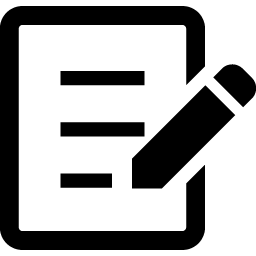
\includegraphics[height=8mm]{figs/assets/certificate.png}\\ \textbf{PLUM-BDEC verification}: succinct STARK receipt \emph{produced}};
      \node[t, below left=15mm and 2mm of root] (bare) {keep the bare STARK receipt};
      \node[t, below right=15mm and 2mm of root] (wrap) {wrap for zero-knowledge (Groth16/PLONK, the only wraps available)};
      \node[t, below=11mm of bare] (noanon) {
\includegraphics[height=8mm]{figs/assets/lock.png}\\ \textbf{not zero-knowledge} $\Rightarrow$ no anonymity};
      \node[t, below left=12mm and -10mm of wrap] (feas) {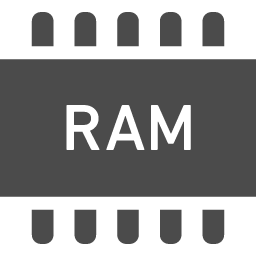
\includegraphics[height=8mm]{figs/assets/memory.png}\\ \textbf{feasible}: the wrap completes within the $24$\,GB budget ($46.83$\,min, peak ${\approx}15$\,GiB)};
      \node[t, below right=12mm and -10mm of wrap] (npq) {
\includegraphics[height=8mm]{figs/assets/shield.png}\\ \textbf{not post-quantum} (pairing-based)};
      \draw[->] (root) -- (bare);
      \draw[->] (root) -- (wrap);
      \draw[->] (bare) -- (noanon);
      \draw[->] (wrap) -- (feas);
      \draw[->] (wrap) -- (npq);
    \end{tikzpicture}
    \caption{The dual obstruction to post-quantum anonymity.}
    \label{fig:dual-obstruction}
\end{figure}

BDEC's anonymity and unlinkability require the underlying argument to be zero-knowledge. The succinct STARK receipt produced by the zkVM is, in the configurations we run, an argument of knowledge but not a zero-knowledge one. SP1's specification states plainly that its STARK proofs are not zero-knowledge~\cite{sp1docs-sec}. We therefore treat the bare receipt as not dependably zero-knowledge, a concrete instance of the caution that a system may be called a zkVM without delivering zero-knowledge. Zero-knowledge is obtained only by wrapping the receipt in a succinct proof, and the wraps SP1 exposes, Groth16 and PLONK, are pairing-based and therefore only classically secure. The obstruction splits into two independent sides, set out below and summarised in Figure~\ref{fig:dual-obstruction}. Both block \emph{post-quantum} anonymity for separate reasons, and naming each one precisely is the security-level result of this analysis.

The first obstruction is that the feasible, post-quantum-sound proof is the bare receipt, which is not zero-knowledge; zero-knowledge is recovered only by wrapping. That wrap completes within the consumer memory budget. The deployable PLONK/BN254 wrap of the PLUM verification proves end-to-end (core, compress, shrink, wrap, and native gnark PLONK, then verify) in $46.83$~min at peak $15.3$~GiB, and the credential-generation wrap in $4.20$~h at peak $15.6$~GiB, both with roughly $8$~GiB of headroom under $24$~GB. What clears the recursion-shape provisioning wall (the static verifying-key tables of Section~\ref{sec:evaluation}) is building a reduced verifying-key map from the guest's own shard shapes, a one-time amortised setup of some $19$--$26$ verifying-key setups completing in tens of seconds, together with the stock v6.1.0 gnark circuit on the sound path (verifying-key checking on), so neither the ${\approx}51$~h regeneration nor a gnark rebuild is needed. The credential-generation wrap's longer wall is a compress tail that scales with the credential's shard count ($1018$ shards against PLUM-verify's $104$), not a memory bound; peak memory stays bounded near $15$~GiB throughout. This completing wrap runs gnark PLONK with the zero-knowledge flag enabled, so it is zero-knowledge by gnark's analysis of that configuration. A dedicated verification run confirms the configuration is active, with two proofs of one witness differing under randomized blinding, and the post-quantum obstruction below holds regardless. The classical anonymity this wrap supplies rests further on the gnark PLONK stage's own knowledge-soundness and on its universal SRS, which the measured runs generate locally rather than through a trusted-setup ceremony. We carry these as benchmark-level properties of the wrapped artifact, not as established guarantees of a deployment. The second obstruction is one of primitives and is the operative one. Wrapping a post-quantum STARK receipt in a pairing-based PLONK or Groth16 proof re-introduces a quantum-vulnerable assumption into the credential's post-quantum soundness, the very class of assumption the post-quantum motivation rules out (Section~\ref{sec:related}). Such a wrap remains acceptable for a classically-secure deployment, and PLONK and Groth16 are not unsuitable in general. They are ruled out here only by the thesis's post-quantum-anonymity goal. Recovering post-quantum anonymity requires a post-quantum-sound zero-knowledge wrap, for instance a STARK-based or lattice-based recursive argument, which the toolchains we run do not yet provide.

The two obstructions differ in kind. The first is not a resource cost at all. The bare receipt is feasible and the pairing wrap that supplies zero-knowledge completes within $24$~GB (Section~\ref{sec:evaluation}), so a deployer who accepts classical security is already served. The second is a primitive limit within the post-quantum goal, since a pairing-based wrap is not post-quantum at any memory or time budget. The first is cleared on this stack; the second bounds what this stack can deliver.

The classically secure PLONK/BN254 wrap therefore gives a deployable \emph{classically}-anonymous configuration, but not a deployable post-quantum-anonymous one. The two obstructions together leave no post-quantum option on the zkVM stack on commodity hardware: the proof that is post-quantum-sound is not anonymous, and the proof that is anonymous is, with the available wraps, only classically secure, whereas a zero-knowledge-enabled Aurora run on the same machine proves the Loquat single-verification building block in about $22$ minutes (mean of three runs, $21.4$--$22.9$; Section~\ref{sec:evaluation}). Within the scope of the literature we surveyed (Section~\ref{ssec:zkvm-proof-security}), we did not find this conjunction stated explicitly for post-quantum anonymous credentials, and surfacing it is a contribution of this thesis: we measure that the zero-knowledge wrap runs within budget and identify the remaining obstruction (the second), the absence of a post-quantum-sound wrap, as a toolchain gap.

The post-quantum gap is scoped to the substrate and hardware studied: an Apple M5~Pro with $24$~GB of memory, the CPU-bound prover of SP1, and the parameter set $\lambda=80$. We do not claim it is fundamental to the primitive or that it persists on server-class hardware. Characterising how it moves with the memory budget and the security level is left as future work.

What would move this gap can be named as three levers. Reaching post-quantum zero-knowledge for this workload requires (i) a post-quantum-sound zero-knowledge wrap in place of the pairing-based ones the toolchains currently expose, for which two hash-based routes already exist as code (masked {FRI} and the {VEIL} compiler; Section~\ref{sec:conclusion}); (ii) that this post-quantum-sound wrap prove within the memory budget, the resource question this thesis leaves open now that the classical pairing wrap is measured to fit; and, for everlasting in place of merely computational anonymity, (iii) a non-interactive, standard-model, statistically-hiding commitment to the witness-bearing trace (Proposition~\ref{prop:everlasting}). Levers (i) and (ii) are engineering questions, the techniques for (i) already implemented and (ii) reducing to whether the masked prover fits the budget; lever (iii) is an open construction problem.

A separate question is the strength of the anonymity guarantee where the argument is zero-knowledge. Two points bound it. The first concerns quantum adversaries. The bound of Equation~\eqref{eq:adv-anon} is stated in the classical random-oracle model, so it constrains a classical distinguisher. Lifting it to the quantum random-oracle model is attainable in principle: the compilation of a round-by-round sound interactive oracle proof into a non-interactive argument is post-quantum secure in the quantum random-oracle model~\cite{cryptoeprint:2019/834}, and this is argued for the {STIR}-class proof systems PLUM uses in recent work~\cite{cryptoeprint:2025/2166}. The lift is not settled here. It remains conditional on a PLUM transcript simulator (Assumption~\ref{asm:szk}) and on a post-quantum analysis of PLUM's own Fiat--Shamir step, which the scheme's published analysis does not provide. We therefore claim computational anonymity against a classical distinguisher and record the quantum lift as attainable but open.

\paragraph{The missing lemma for the quantum lift.}
The quantum-random-oracle lift of PLUM's Fiat--Shamir compilation, recorded above as attainable but open, has a single identifiable missing input: round-by-round, equivalently state-restoration, soundness of PLUM's own multi-round STIR interactive oracle proof at the deployed parameters. The general compilers assume exactly this hypothesis. Chiesa, Manohar and Spooner~\cite{cryptoeprint:2019/834} compile any round-by-round sound IOP into a non-interactive argument secure in the quantum random-oracle model, and the post-quantum BCS-compilation analysis of~\cite{cryptoeprint:2025/2166} delivers adaptive post-quantum soundness from classical round-by-round soundness for the hash-based interactive-oracle proof systems PLUM uses. Neither result asserts that PLUM's particular IOP meets the round-by-round hypothesis at its parameters, and that assertion is the missing lemma.

\begin{conjecture}[Round-by-round soundness of PLUM's STIR IOP at the deployed parameters]\label{conj:rbr-stir}
    PLUM's multi-round STIR-based interactive oracle proof is round-by-round sound with error $\epsilon_{\mathrm{RBR}}$ at the deployed parameters ($\eta=4$, $R=1$, $\kappa_0\in\{16,26\}$, $|U|=2^{12}$, $d^*=128$ the degree bound of the committed polynomial oracle, $\log_2 p\approx199$), in the list-decoding (up-to-capacity) proximity regime. The dominant query-repetition term is fixed by the code rate $\rho=d^*/|U|=128/4096=2^{-5}$: in the capacity regime each of the $\kappa_0$ first-round queries fails with probability about $\rho$, so the query soundness is $\rho^{\kappa_0}=2^{-5\kappa_0}$, giving $2^{-80}$ at $\kappa_0=16$ ($\lambda=80$) and $2^{-130}$ at $\kappa_0=26$ ($\lambda=128$). The full $\epsilon_{\mathrm{RBR}}$ additionally carries STIR's proximity-gap and single folding-round ($R=1$) terms~\cite{cryptoeprint:2024/390}, which we do not reproduce here. Under this conjecture the Fiat--Shamir compilation is quantum-random-oracle secure by~\cite{cryptoeprint:2019/834,cryptoeprint:2025/2166}, lifting EUF-CMA to a quantum forger.
\end{conjecture}

The conjecture is not established for PLUM's specific IOP, and if round-by-round soundness fails at these parameters only the quantum unforgeability lift is lost, while classical EUF-CMA and all anonymity claims are unaffected. The deployed $\kappa_0$ values are worth reading against the regime: at the proven unique-decoding radius each query fails to catch a cheating word with probability about $(1+\rho)/2\approx0.516$, so $\kappa_0=16$ would yield about $2^{-15}$, far short of $\lambda=80$. The parameters therefore presume the conjectured, up-to-capacity proximity regime, and the $2^{-5\kappa_0}$ figure holds only in that regime; this reliance is specific to PLUM's own STIR IOP, unlike the outer SP1 prover's $\epsilon_{\mathrm{KS}}$, whose measured configuration was read above as the proven unique-decoding regime. The up-to-capacity proximity-gaps conjectures this regime rests on were, moreover, recently disproven in their strongest form~\cite{crites2025proximitygaps}, with an unconditional soundness bound above the Johnson bound established only subsequently and at parameters other than ours~\cite{chai2026frijohnson}; the conjectured regime these parameters presume therefore stands on weaker ground than when they were set, reinforcing that the $2^{-5\kappa_0}$ figure is conjectural rather than proven.

\begin{remark}[The anonymity guarantee is computational]\label{rem:everlasting}
    The guarantee is computational, and it is not everlasting: a recorded transcript hides the witness only while the underlying commitment stays hiding. The showing relation itself contains no commitment. The witness enters the zkVM's execution trace, and the prover commits that trace under an algebraic-hash Merkle root, so the receipt binds $w$ through salted evaluations of the schematic form $c = H(w \,\|\, r)$, applied by the proof system rather than by the proved relation. A salted hash leaf hides its input statistically only in the random-oracle model. Once $H$ is a fixed function the hiding rests on a computational assumption on that function, and the random-oracle methodology gives no assurance that the hiding survives the instantiation~\cite{cgh2004rom}. An adversary who stores a transcript and later acquires quantum computing power attacks the instantiated function, against which the hiding is at best computational. Recovering everlasting anonymity would require the trace commitment to be statistically hiding in the standard model and to be non-interactive, since the receipt is a single message. A non-interactive statistically-hiding commitment is not available from general assumptions: any black-box construction from one-way permutations needs $\Omega(n/\log n)$ rounds of interaction~\cite{hhrs2007,wee2007tcc}. Statistical hiding and statistical binding also cannot hold together, so binding must remain computational. The everlasting variant is therefore not currently establishable (the obstruction is formalized as Theorem~\ref{thm:no-everlasting} below).
\end{remark}

\begin{definition}[The hash-committed showing class $\mathcal C$]\label{def:class-C}
    A credential-showing system belongs to the class $\mathcal C$ if its receipt
    satisfies the following four structural conditions.
    \begin{description}
      \item[(C1) Witness carried by a trace hash commitment.] The only component of the receipt that depends on the private witness $w$ and survives the proof's zero-knowledge masking is an algebraic-hash trace root $R$, computed by salted evaluations $\mathsf{com}=H(w\,\|\,r)$ of a fixed public compressing function $H$ over trace data containing $w$, with prover randomness $r$, applied by the proof system rather than by the proved relation. No separate statistically-hiding commitment is applied to $w$ before it enters $H$. The masked opened values are statistically independent of $w$ by the honest-verifier statistical zero-knowledge of the underlying interactive oracle proof~\cite{cryptoeprint:2024/1037}, so $R$ is the sole carrier of $w$.
      \item[(C2) Binding for soundness.] The receipt is knowledge-sound, so $H$ is instantiated as a collision-resistant compression and $R$ binds the committed trace; an accepting receipt therefore certifies a specific authorised witness $w$ rather than a lossy equivalence class of witnesses.
      \item[(C3) Harvest-now adversary.] Everlasting anonymity is anonymity against an adversary who records the single-message receipt and is thereafter computationally unbounded.
      \item[(C4) Random-oracle instantiation.] $H$ is modelled at best as a random oracle; in deployment it is a fixed public function whose description and outputs the adversary of (C3) holds, and no standard-model statistical-hiding property (a leftover-hash-lemma regularity, say) is proven for it.
    \end{description}
    A \emph{masked-STARK} showing, the strongest variant the hash route offers~\cite{cryptoeprint:2024/1037}, lies exactly in $\mathcal C$: its masked opened values are statistically independent of $w$ by honest-verifier statistical zero-knowledge, its witness is bound through the salted trace evaluations $c=H(w\,\|\,r)$ of Remark~\ref{rem:everlasting} under the prover's algebraic-hash Merkle root over its native field, and no statistically-hiding commitment is interposed. The two variants the toolchain actually produces sit below this best case and fail earlier: the bare STARK receipt leaks $w$ through unmasked opened values, and the pairing-based PLONK wrap hides the inner openings only computationally, so neither attains even the statistical masking (C1) presumes. The theorem below therefore bounds the hash route at its strongest point.
\end{definition}

\begin{impossibilitybox}{Non-establishability of everlasting anonymity for $\mathcal C$}\label{thm:no-everlasting}
    Everlasting anonymity cannot be established in the standard model for a system in the class $\mathcal C$ of Definition~\ref{def:class-C} by the routes the class affords: neither $H$'s idealised hiding nor an interposed commitment yields a standard-model statistical-hiding guarantee for the receipt, so the witness-hiding provable for $\mathcal C$ is at most \emph{computational}. The proof invokes no computational hardness assumption and grants the adversary unbounded power; it claims no universal impossibility beyond the class structure (Remark~\ref{rem:thaler-boundary}).
\end{impossibilitybox}

\begin{proof}
    Everlasting anonymity requires that the recorded receipt be statistically independent of $w$, so that the unbounded distinguisher of (C3) gains no advantage. By (C1) the receipt's only $w$-dependent surviving component is the trace root $R$, a commitment computed by the fixed function $H$ through $\mathsf{com}=H(w\,\|\,r)$; establishing everlasting anonymity for a system in $\mathcal C$ therefore requires exhibiting a standard-model statistical-hiding guarantee for $R$. Such a guarantee must be a property either of $H$ itself or of a structure interposed before $H$; these are the only two routes, and both are closed. The first is closed by (C4): $H$'s statistical hiding is an artefact of the idealisation, and no standard-model hiding property is proven for the deployed function (a fixed $H$ with, say, a proven leftover-hash-lemma regularity would fall outside (C4)). The second is closed by (C1) and the one-message form of the receipt, as the next two paragraphs detail.
    
    The statistical hiding that $H$ does enjoy is an artefact of the random oracle. A salted leaf $H(w\,\|\,r)$ hides its input statistically when $H$ is an ideal random oracle, with distinguishing advantage at most $q/(2^\lambda-q)$ for $q$ queries; this is the elementary random-oracle collision-and-hit bound, holding only in the idealised model. By (C4) the deployed $H$ is a fixed public function, and the random-oracle methodology gives no assurance that a property proved relative to the oracle survives the instantiation~\cite{cgh2004rom}. The harvest-now adversary of (C3) does not query an oracle; it holds the recorded digest $R$ and the public function $H$, and attacks the instantiation, against which the random-oracle hiding argument transfers nothing.
    
    The remaining route to statistical hiding, a non-interactive standard-model statistically-hiding commitment applied to $w$ before it reaches $H$, is excluded from $\mathcal C$ by (C1). It is moreover not available from general assumptions for a single-message receipt: any black-box construction of a statistically-hiding commitment from one-way permutations requires $\Omega(n/\log n)$ rounds of interaction~\cite{hhrs2007,wee2007tcc}, whereas the receipt is one message, so no commitment obtained from these general-assumption constructions can be interposed.
    
    No route open to $\mathcal C$ yields a standard-model statistical-hiding guarantee for $R$: the random-oracle hiding of (C4) does not transfer to the instantiation by the argument of~\cite{cgh2004rom}, and by (C1) the receipt interposes no separate statistically-hiding commitment, and none is available to a one-message receipt from general assumptions. Consequently $\mathcal C$ affords no standard-model argument that its receipt is statistically independent of $w$, so any provable witness-hiding for a system in $\mathcal C$ is at most computational, and reading Equation~\eqref{eq:adv-anon} in the everlasting setting its $\epsilon_{\mathrm{ZK}}$ term is not statistical and is not established small against the unbounded distinguisher of (C3). No step assumes any function is hard to invert; the obstruction is that the only hiding $\mathcal C$ provably affords in the standard model is computational, and against the unbounded adversary of (C3) computational hiding carries no established guarantee. Everlasting anonymity therefore cannot be established in the standard model for any system in $\mathcal C$; whether some system in $\mathcal C$ nonetheless happens to be everlastingly anonymous is left open.
\end{proof}

\begin{remark}[The computational boundary]\label{rem:thaler-boundary}
    Theorem~\ref{thm:no-everlasting} does \emph{not} claim that computational anonymity fails. Under the zero-knowledge assumption (Definition~\ref{def:zk}) the commitment $\mathsf{com}=H(w\,\|\,r)$ is computationally hiding, so the showing is anonymous against a bounded classical distinguisher, at advantage $\mathsf{Adv}^{\mathsf{anon}}\le(k+2)\,\epsilon_{\mathrm{sZK}}+\epsilon_{\mathrm{ZK}}$ of Equation~\eqref{eq:adv-anon}, once a zero-knowledge wrap makes $\epsilon_{\mathrm{ZK}}$ small. The non-establishability is confined to the everlasting, statistical strengthening for the class $\mathcal C$. The harvest-now, de-anonymise-later harm therefore attaches to transcripts \emph{in} $\mathcal C$ because their hiding is computational; it is not a claim that every recorded zero-knowledge proof must be post-quantum, only that a receipt whose witness-hiding is a bound hash commitment to the execution trace inherits a computational, not everlasting, guarantee.
    
    The theorem is a non-establishability result \emph{for the class}, not a universal impossibility, and the boundary of $\mathcal C$ is the escape route. Interposing a non-interactive standard-model statistically-hiding commitment to $w$ before $H$ leaves $\mathcal C$ and reaches everlasting anonymity, which is exactly the hypothesis of Proposition~\ref{prop:everlasting}. This route is realisable as shown by the everlasting anonymous rate-limited tokens of Chairattana-Apirom, D\"ottling, Lysyanskaya and Tessaro~\cite{cryptoeprint:2025/1030}, which achieve everlasting anonymity through a statistically-hiding pairing-based commitment, at the cost of classical, non-post-quantum soundness and only within a rate limit. Their construction is consistent with the theorem rather than a counterexample to it: everlasting anonymity is attained precisely by leaving the hash-only class $\mathcal C$, and on this evidence the achievable route is pairing-based rather than post-quantum. This is the same seam the dual obstruction of Proposition~\ref{prop:wall} records, read now at the information-theoretic level.
\end{remark}

\begin{proposition}[Conditional everlasting anonymity]\label{prop:everlasting}
    Suppose there is a non-interactive, post-quantum, statistically-hiding commitment to the witness columns of the trace that composes with the low-degree test, so that the witness is committed before it enters the algebraic-hash root and the proximity test does not re-expose it. Then, in a masked variant of the proof and under the hypotheses of Theorem~\ref{thm:security-preserve}, with Assumption~\ref{asm:szk} taken in its \emph{statistical} form (the transcript-simulation error $\epsilon_{\mathrm{sZK}}$ a statistical distance; Definition~\ref{def:szk} as stated quantifies only over efficient distinguishers), the zkVM-executed BDEC system is everlastingly anonymous and unlinkable: against an unbounded distinguisher the advantage is at most $\epsilon_{\mathrm{ZK}}^{\mathrm{stat}} + (k+2)\,\epsilon_{\mathrm{sZK}}$ for anonymity and $\epsilon_{\mathrm{ZK}}^{\mathrm{stat}} + \epsilon_{\mathrm{sZK}}$ for unlinkability, where $\epsilon_{\mathrm{ZK}}^{\mathrm{stat}}$ is statistical. Binding, and hence unforgeability, remains computational.
\end{proposition}

\begin{proof}[Proof sketch]
    The anonymity argument of the preservation theorem is unchanged except at the step that hides the witness in the trace commitment. In the construction analysed that step is computational, because the witness columns sit under a collision-resistant Merkle root (Remark~\ref{rem:everlasting}). Under the hypothesised commitment the witness columns are statistically hidden before they reach the root, so the root carries no statistical information about the witness, and the low-degree test operates on the committed columns without re-exposing it. The masked interactive oracle proof is statistically honest-verifier zero-knowledge by randomisation, independently of the hash~\cite{cryptoeprint:2024/1037}, so the transition incurs only the statistical distance $\epsilon_{\mathrm{ZK}}^{\mathrm{stat}}$, and the transcript-simulation step is unchanged, its $\epsilon_{\mathrm{sZK}}$ now the statistical distance of the strengthened assumption, at cost $(k+2)\,\epsilon_{\mathrm{sZK}}$ for anonymity and $\epsilon_{\mathrm{sZK}}$ for unlinkability. An unbounded distinguisher therefore gains at most $\epsilon_{\mathrm{ZK}}^{\mathrm{stat}} + (k+2)\,\epsilon_{\mathrm{sZK}}$ for anonymity, and $\epsilon_{\mathrm{ZK}}^{\mathrm{stat}} + \epsilon_{\mathrm{sZK}}$ for unlinkability. Binding stays computational, since a commitment cannot be both statistically hiding and statistically binding, so the unforgeability bound is unaffected.
\end{proof}

A concrete candidate for the hypothesised commitment is the Module-{SIS}-based commitment of Baum, Damg{\aa}rd, Lyubashevsky, Oechsner and Peikert~\cite{bdlop2018}, which is statistically hiding in a parameter regime that trades off against binding. It is post-quantum, but its proof of opening is interactive, so it does not by itself meet the non-interactive requirement above. Closing that gap is the open problem behind Proposition~\ref{prop:everlasting}.

This closes the chapter on the terms its opening set. Of the three conditions of Definition~\ref{def:deployable}: knowledge soundness transfers conditionally (Theorem~\ref{thm:security-preserve}, modulo Assumptions~\ref{asm:air} and~\ref{asm:lookup} and Conjecture~\ref{conj:extract-recursion}); zero-knowledge is delivered within the memory budget by the pairing wrap, against a classical distinguisher; and post-quantum anonymity remains blocked by the second obstruction alone, the toolchain gap to which this section has reduced the dual obstruction.
 
    \newpage
    \section{Evaluation}\label{sec:evaluation}
This section reports what the precompile-enabled zkVM regime can and cannot do for PLUM-based BDEC on consumer hardware, and reads the measurements back against the cost framework of Section~\ref{sec:theoretical}. Four findings answer the thesis's question, one per contribution. \emph{Feasibility}: the Griffin precompile turns PLUM verification from a non-terminating run into a $14.24$-minute proof within the $24$~GB envelope (Table~\ref{tab:plum-verify}). \emph{The cost criterion}: that precompiled hash nonetheless proves slower than a software SHA-3 control ($14.24$ versus $13.24$~min), an inversion whose sign the trace-area model postdicts. The measured evidence gives three results (the design-level field-multiplication verdict is Section~\ref{sec:system}'s). Griffin removes $58.5\times$ cycles yet loses on committed area. The matched-field control confirms the necessity direction ($164\times$ tax, execute mode). The power-residue symbol pays $10.33\times$ on total committed area (\S\ref{ssec:attribution}, \S\ref{sssec:already-served}). \emph{The credential characterisation}: both credential relations run and prove on SP1 (Table~\ref{tab:bdec}). \emph{The dual obstruction}: the zero-knowledge wrap completes in $46.83$~minutes but is pairing-based and so classical, not post-quantum (\S\ref{ssec:resource-frontier}). Within the scope of the literature we surveyed these are among the first such figures; the configurations that do not complete are reported alongside those that do, and everything that follows is the evidence for these four.

\subsection{Setup and Methodology}\label{ssec:eq}
We measure PLUM verification and the credential relations built on it with and without the precompile suite, attribute where the zkVM cost falls and how much the suite removes, locate the resource boundary for the configurations that do not complete, and compare the zkVM and static-circuit regimes on update churn (Definition~\ref{def:update-churn}).

\paragraph{Two measurement modes.}
\emph{Execute mode} counts RISC-V cycles without producing a proof; its cost is machine-independent and always terminates. \emph{Prove mode} produces the receipt, is the deployment-relevant cost, and does not always complete on the target hardware. We therefore report prove wall-clock where proving completes and fall back to execute-mode cycles where it does not, never comparing the two across that boundary; each table states its mode. \emph{Feasible} means the prove completes within the $24$~GB envelope; whether a completed time is \emph{acceptable} is a separate judgment this chapter does not make: the deployment trade-offs it turns on are weighed in Section~\ref{sec:discussion}, and the operational bar the thesis does and does not state is fixed in Section~\ref{sec:conclusion}.

\paragraph{What we do not claim.}
We report no single ``$N\times$ speedup.'' The with/without-precompile contrast at the prove level is an \emph{infeasible-to-feasible} transition, not a ratio of two finite times (\S\ref{ssec:headline}); the finite reductions we report are cycle-level, at a stated security level and mode.

\paragraph{Platform.}
Table~\ref{tab:platform} lists the evaluation platform; all prove-mode measurements are local single-machine runs with no network or dev-mode acceleration unless stated.

\begin{table}[H]
\centering
\small
\begin{tabular}{ll}
\toprule
Component & Specification \\
\midrule
Hardware & Apple M5~Pro, 18-core CPU, 20-core GPU, 24~GB unified memory, 1~TB SSD \\
OS & macOS 26.5 (Darwin 25.5.0), Apple Silicon (arm64) \\
Prover & CPU-bound; no CUDA/network prover (Apple Silicon has no NVIDIA GPU path) \\
zkVM & SP1 v6.2.1 (forked) \\
Signature & PLUM over $\mathbb{F}_p$, $p=2^{64}p_0+1$ ($199$-bit; see \S\ref{ssec:bigint}) \\
Security levels & $\lambda=80$ (prove-mode runs; Griffin-delta and credential execute figures), $\lambda=128$ (cost-attribution analysis, \S\ref{ssec:attribution}) \\
\bottomrule
\end{tabular}
\caption{Evaluation platform and measurement setup.}
\label{tab:platform}
\end{table}

\subsubsection{Settings Justification}\label{ssec:settings-justify}
Each fixed parameter is one a deployer would plausibly choose; we disclose where a setting is tuned.

\begin{description}
  \item[Consumer hardware (M5~Pro, 24~GB).] The research question concerns deployability on a personal machine, so this hardware is the thesis's explicit scope. Every feasibility claim is scoped to this envelope and is not asserted in general.
  \item[Security level: $\lambda=80$ for prove-mode, $\lambda=128$ for cycle attribution.] We disclose this seam. Prove-mode runs use $\lambda=80$ because $\lambda=128$ proving is untested and expected to exceed the memory budget, the precompile-free arm already failing at $\lambda=80$ (Table~\ref{tab:plum-verify}). $\lambda=80$ is the largest level at which prove-mode wall-clock is observable on this hardware, which is why we use it and not because it is favourable. The cost-attribution analysis (\S\ref{ssec:attribution}) is reported at the audience-relevant $\lambda=128$ because it is machine-independent (execute mode) and so remains measurable where proving is not. No number mixes the two levels silently. Each table states $\lambda$.
  \item[Prover memory tuning.] At SP1's default settings the Cell~2 prove is OOM-killed after ${\approx}3$~min on the $24$~GB machine. A documented reduced-memory configuration (\texttt{SHARD\_SIZE}$\,=2^{22}$, default $2^{24}$; \texttt{ELEMENT\_THRESHOLD}$\,=2^{26}$; \texttt{HEIGHT\_THRESHOLD}$\,=2^{20}$; \texttt{TRACE\_CHUNK\_SLOTS}$\,=2$; \texttt{RAYON\_NUM\_THREADS}$\,=8$, default $18$; \S\ref{ssec:repro}) trades smaller, more numerous shards and fewer threads for fitting the envelope, so the headline timings are tuned-configuration times (Cell~2 $14.24$~min, SHA-3 control $13.24$~min under identical tuning; the zero-knowledge wrap ${\approx}15$~GiB peak, \S\ref{ssec:resource-frontier}). One contributing factor to the Griffin arm's memory pressure: the fork's shard-budgeting table prices the Griffin chip at $348$ trace columns against its compiled $3{,}819$, so a Griffin-bearing shard is budgeted at roughly a tenth of its committed area and split later than the trace-area threshold intends; correcting the entry is a one-line change whose effect on Cell~2 is untested and left to future work.
  \item[Micro-benchmark isolation.] Cost-attribution runs isolate single primitives (one Griffin permutation; one verification) so that per-operation cost can be attributed rather than inferred from an aggregate.
\end{description}

\subsubsection{Reproducibility}\label{ssec:repro}
Prove-mode and attribution runs use fixed RNG seeds and fixed messages. The SP1 submodule version is pinned in the lockfile. The memory-tuning environment variables, host binaries, and the adversarial-probe harness are recorded in the project's measurement notes, together with the per-run commit hashes and, where applicable, guest-image identifiers. The exception is an earlier, retired pair of CreGen prove runs (the $26.98$/$27.45$~min pair; \S\ref{ssec:frontier}): their shard configuration was recorded only in a human-written summary rather than machine-echoed in the run log, and does not reproduce on the shipped fork. The credential-relation prove figures of Table~\ref{tab:bdec} are the config-verified runs of \S\ref{ssec:frontier}.

\subsection{PLUM Verification With and Without the Precompile}\label{ssec:headline}

Table~\ref{tab:plum-verify} reports prove-mode results for a single PLUM signature verification at $\lambda=80$. The central comparison is between the precompile-free baseline and the precompile-enabled arm on the same hardware. Its rows label Cell~1/2/3 as no precompile / Griffin precompile / SHA-3 control, and the control is not a deployable variant.

\begin{table}[H]
\centering
\small
\begin{tabular}{lllll}
\toprule
zkVM / mechanism & $\lambda$ & Prove time & Peak mem & Outcome \\
\midrule
Cell~1: SP1, rv64im Griffin (no precompile)  & 80 & n/a       & ${\approx}13.6$~GiB & DNF (stopped at $5$\,h\,$07$\,m) \\ % Cell 1 tuned; master_batch_20260706 C1e (watchdog 1200s cap, peak 13.62 GB, well under 24 GB)
\textbf{Cell~2: SP1, Griffin-$\mathbb{F}_p^{192}$ precompile (this work)} & \textbf{80} & \textbf{14.24~min}\textsuperscript{\dag} & \textbf{${\approx}13.7$~GiB} & \textbf{receipt verified} \\          % 582ad1a Cell 2 (this work, emphasized); n=5 master_batch_20260706
Cell~3: SP1, SHA-3 hasher (control)          & 80 & 13.24~min\textsuperscript{\dag} & ${\approx}14.4$~GiB & receipt verified \\ % 91941ed; n=5 master_batch_20260706
\bottomrule
\end{tabular}
\caption{PLUM verification, prove mode ($\lambda=80$; the Griffin instance runs at $14$ rounds, one below the security-conservative $15$ of Table~\ref{tab:round-margin}).}
\label{tab:plum-verify}
\end{table}

A run of the precompile-free arm under the documented reduced-memory tuning (\S\ref{ssec:settings-justify}) ran for $5$\,h\,$07$\,m without terminating and without exhausting memory before we stopped it by hand, yielding no receipt. Under that tuning the binding resource is time rather than memory, and the prove still does not complete within five hours on this hardware.

\paragraph{The honest reading.}
The with/without-precompile contrast is not a ratio of two finite times. Without the precompile the workload \emph{does not complete} on this hardware, and with it the workload completes in $14.24$~minutes (mean of five runs, $14.16$--$14.44$). The defensible claim is therefore qualitative at the prove level (\emph{the precompile moves PLUM verification from infeasible to feasible on consumer hardware}) and quantitative only at the cycle level (\S\ref{ssec:attribution}).

The SHA-3 control does not isolate the hash family (it differs from the Griffin arm in two things at once, the hash (bit-oriented SHA-3 against $\mathbb{F}_p^{192}$ Griffin) and the field, matched only on the security level $\lambda$, so it is a deliberately confounded control rather than a hand-picked favourable setting). The verification harness is identical except that every Griffin-$\mathbb{F}_p^{192}$ sponge call is replaced by a SHA3-256 call computed in software, so that the SHA-3 arm fires \emph{no} hash precompile and only the shared \texttt{UINT256\_MUL} field-multiplication precompile remains active. It shows that a workload using a \emph{standard} hash in software is cheaper, by the margin the next paragraph quantifies, than one using the algebraic hash PLUM requires through a bespoke chip, which is the quantitative form of the field-mismatch-tax argument of Section~\ref{sec:theoretical}.

The inversion is direct. The bespoke Griffin-$\mathbb{F}_p^{192}$ precompile proves \emph{slower} at prove than the software SHA-3 control at matched $\lambda=80$ in every run we took. The sign is robust. At a fixed tuned config on a clean machine, five Cell~2 runs and five Cell~3 runs give means of $14.24$~min (range $14.16$--$14.44$) and $13.24$~min (range $13.02$--$13.38$), a magnitude of ${\approx}1.08\times$ in wall-clock and ${\approx}1.11\times$ in cycles, with each arm's prove-time spread under $5\%$. An earlier single run measured $32.53$ versus $13.28$~min; its high Cell~2 figure was not reproduced under fixed-config replication and is attributed to machine-state contamination rather than an intrinsic build difference, so the reported value is the replicated $14.24$~min.

\paragraph{Why the model postdicts the sign.}
We read the inversion as a genuine property of the pipeline rather than a measurement artefact, and the trace-area accounting of Section~\ref{sec:theoretical} (Equation~\eqref{eq:trace-area-model}) postdicts its sign from the chips' committed dimensions. The Griffin chip emits $14$ rows of $3{,}819$ columns per permutation (each row carries $26$ modular-arithmetic gadgets of $127$ cells each, beside range checks and state limbs), so the $1{,}052$ permutations of one verification commit $14\times 3{,}819\times 1{,}052\approx 5.6\times10^{7}$ cells, plus one controller row per permutation, that the SHA-3 arm never pays. The shared \texttt{UINT256\_MUL} chip is common-mode ($69{,}396$ versus $69{,}385$ events) and cancels, and the Griffin arm additionally executes $11\%$ more guest cycles ($1.23\times10^{8}$ versus $1.11\times10^{8}$, execute mode). Both terms of Equation~\eqref{eq:trace-area-model} are therefore larger on the Griffin arm, so the model places it behind the control for every non-negative choice of the per-cell rates, granted a common per-cycle core area across the two arms. The calibration of the model's constants on these two arms is reported with the cost model (\S\ref{ssec:costmodel}). The feasibility recovery and the inversion are the same cost model (Equation~\eqref{eq:trace-area-model}) evaluated at two operating points. With the precompile the run completes and can be measured, and the cost model explains why it is still no faster than the control. The control's hash costs the substrate no chip area at all, while the Griffin arm pays for its chip and saves nothing in return.

Not all of that width is irreducible. Of the twenty-six field operations per row, about ten are genuine $192$-bit multiplications, the S-box arithmetic that no small field avoids. The other sixteen are additions and small linear combinations. They are charged at the full multiplication price only because the chip reuses one circuit for both, so a dedicated addition path would cut about a quarter of each row. Even so trimmed, every remaining cell still computes over the $199$-bit field, so a leaner chip narrows the gap toward parity but does not reverse its sign against a hash whose cost is field-invariant.

The inversion is moreover conservative twice over. The SHA-3 control runs in software with no chip of its own, so a native bit-hash precompile would only widen the gap, and the Griffin instance is arithmetised at $14$ rounds against the $15$ its parameters call for (Section~\ref{sec:security}, Table~\ref{tab:round-margin}), so a correctly-secure instance adds roughly another fourteenth of the Griffin cells and widens the gap further.

\paragraph{Proof size, and the wrap that produces it.}
Receipt size in SP1 is a property of the proof \emph{type}, not of the workload. The runs above use SP1's default \emph{core} proof, whose size \emph{scales with execution size}~\cite{succinct2025prooftypes}. The compact, on-chain-deployable proof is instead the constant-size {SNARK} \emph{wrap} of that receipt, about $260$~bytes for Groth16 over {BN254}, or $868$~bytes for {PLONK}~\cite{succinct2025prooftypes}. Producing that wrap completes on the target hardware: the full sound {PLONK}/{BN254} chain wraps one PLUM verification into a verified constant-size proof in $46.83$~minutes at a $15.29$~GiB peak, inside the $24$~GB budget and without the default path's multi-day regeneration (\S\ref{ssec:resource-frontier}). On a $24$~GB machine the deployer can therefore generate either the large, shard-scaling core receipt or the $260$-to-$868$-byte {SNARK} wrap of it; the post-quantum gap that wrap leaves is taken up in \S\ref{ssec:resource-frontier}. We report the wrapped figure as measured and do not serialise the workload-dependent core receipt, whose byte count is not the deployment-relevant number.

\paragraph{An empirical witness leak on the non-zero-knowledge core path.}
The core receipt's workload-dependence is not merely formal. Fixing the relation and varying only the witness across $N=20$ standalone PLUM verifications, the Griffin permutation count is witness-invariant at $1{,}052$, while the field-multiplication count and the total cycle count vary from witness to witness (execute mode). The variation reaches the verifier-observable proof. Three prove-mode runs on distinct witnesses ($N=3$) produce core receipts of $154.67$, $156.12$, and $153.21$~MB, all distinct, a ${\approx}1.9\%$ spread. Because the shipped core STARK is not zero-knowledge (\S\ref{ssec:resource-frontier}), this leak is on a path where no anonymity is claimed. A constant-size zero-knowledge SNARK wrap removes it, its byte count being independent of the witness (about $260$~bytes for Groth16 over BN254, $868$ for PLONK; Figure~\ref{fig:proof-collapse}). That wrap completes on this hardware (\S\ref{ssec:resource-frontier}), so on the wrapped path the leak closes. What it does not close is post-quantum security, because that wrap rests on a {BN254} pairing (\S\ref{ssec:resource-frontier}): the leak's fix and the anonymity gap are the same wrap seen from two sides.

\begin{figure}[H]
\centering
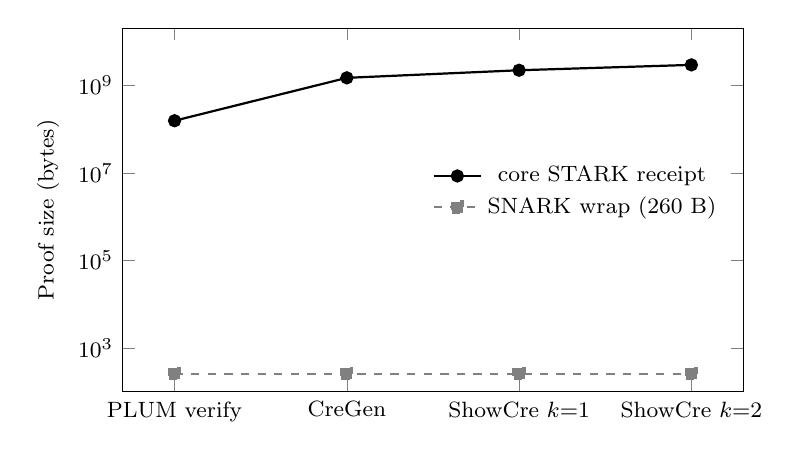
\begin{tikzpicture}
\begin{axis}[
  width=0.78\textwidth, height=6.2cm,
  ymode=log, log basis y={10},
  ylabel={Proof size (bytes)},
  symbolic x coords={PLUM verify, CreGen, ShowCre $k{=}1$, ShowCre $k{=}2$},
  xtick=data,
  ymin=1e2, ymax=2e10,
  tick label style={font=\footnotesize}, label style={font=\footnotesize},
  x tick label style={font=\footnotesize},
  legend style={font=\footnotesize, at={(0.98,0.55)}, anchor=east, draw=none, fill=none},
  clip=false,
]
\addplot[mark=*, black, thick] coordinates {
  (PLUM verify, 154665328) (CreGen, 1473690434) (ShowCre $k{=}1$, 2195116844) (ShowCre $k{=}2$, 2911822343)
};
\addlegendentry{core STARK receipt}
\addplot[mark=square*, gray, dashed, thick] coordinates {
  (PLUM verify, 260) (CreGen, 260) (ShowCre $k{=}1$, 260) (ShowCre $k{=}2$, 260)
};
\addlegendentry{{SNARK} wrap ($260$~B)}
\end{axis}
\end{tikzpicture}
\caption{Within-pipeline proof-size collapse (same scheme, same runs).}
\label{fig:proof-collapse}
\end{figure}

\subsection{Cost Attribution}\label{ssec:attribution}
To attribute the cost we use execute-mode cycle counts at $\lambda=128$, the audience-relevant security level, where prove-mode is infeasible but cycle counts remain machine-independent. Table~\ref{tab:ablation} reports the cumulative effect of routing PLUM's field arithmetic through the host precompile, as an ablation over the SHA-3-hasher verification path.

\begin{table}[H]
\centering
\small
\begin{tabular}{lrr}
\toprule
Configuration (cumulative) & SP1 cycles & $\Delta$ vs.\ baseline \\
\midrule
Baseline (\texttt{BigUint} emulation)        & 289{,}778{,}709 & n/a \\
$+$ field mul via host precompile            & 276{,}643{,}994 & $-4.5\%$ \\
$+$ power as square-and-multiply             & 240{,}857{,}140 & $-16.9\%$ \\
$+$ skip redundant reduction                 & 179{,}952{,}920 & $-37.9\%$ \\
\bottomrule
\end{tabular}
\caption{Cycle-level cost attribution of the field-arithmetic optimizations.}
\label{tab:ablation}
\end{table}

\paragraph{Where the cost lives, and the parameter-set caveat.}
At $\lambda=128$ a single PLUM verification on the SHA-3-hasher arm issues about $112{,}902$ $\mathbb{F}_p^{192}$ multiplication syscalls through the host precompile, as counted in our own SP1 run log. No Griffin permutation executes on that arm, so this figure measures the verifier's \emph{non-hash} field arithmetic (PLUM \S4.2 reports $\approx 10^4$ non-hash algebraic R1CS constraints, $10{,}333$ of $116{,}285$). The Griffin-internal multiplication cost appears instead in the with/without-AIR contrast at $\lambda=80$. The software-Griffin arm fires $4{,}870{,}724$ \texttt{UINT256\_MUL} syscalls against $69{,}396$ with the Griffin AIR active, the hash-internal field operations either absorbed by the \texttt{GRIFFIN\_FP192\_PERMUTE} syscall or inflating the multiplication count $70\times$. The contrast is therefore consistent with the field-mismatch cost model. The cost is dominated by the algebraic hash, whose internal field operations leave the syscall stream only when the bespoke chip absorbs them. We caution explicitly against transferring the PLUM paper's circuit-SNARK figure (that $91\%$ of \emph{R1CS constraints} are hash work) directly to the zkVM cost model. That figure is a constraint count in a different proving system, whereas Table~\ref{tab:ablation} is a RISC-V cycle count. The qualitative conclusion (hash/field arithmetic dominates) agrees. The exact share differs by cost model and is reported here in the zkVM's own units.

\paragraph{Execute-mode delta for the Griffin precompile (PLUM-80).}
For the bespoke Griffin AIR specifically, the precompile-free versus precompile-enabled execute-mode cycle counts differ by a factor of $58.5\times$ at $\lambda=80$, the ratio of precompile-free to Griffin-AIR-enabled cycles on the Griffin arm. This is close to the field-mismatch tax of Proposition~\ref{prop:fmt-lb}. It exceeds the schoolbook $\ell^2\approx 49$ per-multiplication estimate because the whole Griffin permutation collapses into a single precompile call, rather than being emulated one multiplication at a time. This is distinct from the $37.9\%$ of Table~\ref{tab:ablation}, a separate field-multiplication-reduction ablation reported at $\lambda=128$. 
We report this as an \emph{execute-mode cycle ratio} rather than a wall-clock speedup. It is the machine-independent counterpart of the infeasible-to-feasible prove transition of Table~\ref{tab:plum-verify}, and it is the figure that should be cited when a single number is wanted, in place of any prove-time ``speedup,'' which is undefined when the baseline does not complete.

\subsection{The Credential Relations and the Consumer-Hardware Frontier}\label{ssec:frontier}
Moving from a single signature to the credential-generation relation $R_{\mathsf{cre}}^{\Sig}$ instantiated with PLUM (two signature verifications under a hidden user key; \S\ref{ssec:integration}), Table~\ref{tab:bdec} reports the application-level results at $\lambda=80$. These are execute-mode cycle counts and SP1 succinct-prove-mode wall-clock for both credential relations.

\begin{table}[H]
\centering
\small
\begin{tabular}{l l p{3.2cm} p{4.6cm}}
\toprule
Workload & Mode & Cost & Outcome \\
\midrule
CreGen & execute & $9.12\times10^{10}$ cyc & both verifications accept \\ % SP1 software-Griffin, sp1_bdec_execute_20260707 (91,177,673,619 cyc, standard-Griffin)
CreGen, SP1 & prove (succinct) & $68.96$~min ($1.47$~GB proof, $n{=}1$) & succinct receipt verified \\ % config-verified HEIGHT_THRESHOLD=2^16
ShowCre $k{=}1$, SP1 & prove & $103.34$~min ($2.2$~GB proof, $n{=}1$) & succinct receipt verified \\
ShowCre $k{=}2$, SP1 & prove (succinct) & $136.82$~min ($2.9$~GB proof, $n{=}1$) & succinct receipt verified \\
\bottomrule
\end{tabular}
\caption{Credential relations: execute and prove-mode cost ($\lambda=80$).}
\label{tab:bdec}
\end{table}

The execute-mode result validates the honest path of the BDEC credential relation end-to-end inside the zkVM. Both signature verifications accept, at $9.12\times10^{10}$ cycles. The CreGen prove figure of Table~\ref{tab:bdec} is the config-verified reproducible completing prove, $68.96$~min ($1.47$~GB proof) at \texttt{HEIGHT\_THRESHOLD}$=2^{16}$; an earlier $26.98$/$27.45$~min ($296$~MB proof) pair was faster but its shard configuration was recorded only in a human-written summary, not machine-echoed, and does not reproduce on the current fork, so it is not used. The ShowCre figures are likewise the config-verified reproducible completing proves at $k{=}1,2$. Rejection behaviour was probed only at single-verification scope (Section~\ref{sec:system}). On SP1 both credential relations complete a succinct (non-zero-knowledge) prove (Table~\ref{tab:bdec}); the credential-generation wrap and both the $k{=}1$ and $k{=}2$ showing wraps complete and verify within the memory budget, the $k{=}2$ wrap statement-bound.

\paragraph{Both relations bind their public statement.}
The proves of Table~\ref{tab:bdec} are outcome-only. A statement-bound variant additionally commits each relation's public statement to the receipt journal and recovers it on verification. A statement-bound CreGen prove completes in $66.05$~min, accepting, with the committed $x_{\mathsf{cre}}=(c,h,\mathsf{ppk})$ recovered and matched against the input; a full end-to-end run binds the showing as well, with two cross-issuer CreGen issuances ($66.14$ and $65.59$~min) and a $k{=}2$ ShowCre presentation ($127.94$~min) each accepting, its committed statement recovered and matched, the presentation binding $x_{\mathsf{show}}=((\mathsf{ppk}_{\mathsf{TA}})_j,\mathsf{ppk}_{UV},h_{UV})$ while keeping the shown credential private. Binding composes with the zero-knowledge wrap in a single run: a statement-bound CreGen wrap (the jbind guest of Section~\ref{sec:system} through the full chain of \S\ref{ssec:resource-frontier}) completes and verifies in $4.18$~h at a $15.2$~GiB peak, and the showing wrap likewise (the statement-bound $k{=}2$ figure in \S\ref{ssec:costmodel}), so both credential relations carry a measured statement-bound zero-knowledge wrap. The commitment cost is not separately resolvable: the bound CreGen prove ($66.05$~min) and wrap ($4.18$~h) each land within a few percent of their outcome-only counterparts ($68.96$~min, Table~\ref{tab:bdec}; $4.20$~h, \S\ref{ssec:resource-frontier}); both sides are single runs, so this is closeness between two runs rather than a variance-resolved bound, and binding is indistinguishable from free at single-run resolution.

\subsubsection{The post-quantum frontier}\label{ssec:resource-frontier}
The zero-knowledge wrap of a PLUM proof completes on the target hardware. The full sound chain (core, compress, shrink, wrap to {BN254}, and a native gnark {PLONK} proof of the fixed wrap circuit, with verifying-key verification on throughout) produces a verified constant-size proof of one PLUM single-signature verification (Cell~2 of Table~\ref{tab:plum-verify}, the $14.24$-min core prove) in $46.83$~minutes at a peak of $15.29$~GiB, inside the $24$~GB envelope with ${\approx}8.7$~GiB to spare. The credential relation wraps too. A full CreGen zero-knowledge wrap completes in $252$~minutes ($4.20$~h) at a $15.63$~GiB peak. Neither is memory-bound.

The wrap avoids the multi-day artifact regeneration the toolchain's default path implies. On the default path the wrap is killed at the recursive-compression step, because SP1's static recursion-shape and verifying-key tables are provisioned for smaller relations than PLUM verification, and rebuilding those tables in full is a one-time ${\approx}51$~h compute over $185{,}862$ entries (projected from a measured per-setup slope of ${\approx}1$~s across contiguous slices at the start, middle, and end of the table, \rr{docs/measurements/zkwrap_vkmap_slope_20260628}; the rebuild itself was never run, being exactly what the reduced table avoids). We circumvent that rebuild rather than pay it. The wrap verifies against a \emph{reduced} verifying-key table built from only the guest's own shard shapes ($19$ setups in $31$~s for PLUM verification, $26$ setups in $41$~s for CreGen) together with SP1's stock wrap circuit, which reuses the shipped {BN254} gnark circuit unchanged. The sound path is preserved (verifying-key verification stays on), so no recursion-shape rebuild and no circuit rebuild is needed. The gnark {PLONK} stage runs with its zero-knowledge blinding enabled, confirmed by a dedicated check in which two proofs of one witness differ under randomized blinding (\rr{docs/measurements/wrap_zk_check_20260707}). The pipeline's completion and its verifier acceptance are likewise measured. The post-quantum gap below holds independently of that check.

What the wrap does \emph{not} provide is post-quantum anonymity. The wrap rests on a {BN254} pairing, so the zero-knowledge it confers is classical-computational, sound against a classical distinguisher but not against a quantum one. A post-quantum-anonymous proof would need a post-quantum-sound recursive zero-knowledge wrap, which this toolchain does not offer. The provisioning wall therefore does not bind here; what does is the dual obstruction, whose analysis is Section~\ref{sec:security}'s and whose deployment reading is Section~\ref{sec:discussion}'s. The substrate can produce a zero-knowledge proof (over a classical pairing) or a post-quantum proof (the non-zero-knowledge core receipt), and not, as it ships, one proof that is both: the anonymity--deployability tension takes its measured form here.

A second and separate cost governs the wrap's \emph{wall-clock}, and it grows with the credential. The compress stage dominates the wrap tail and scales with the core proof's shard count. PLUM verification's $104$ shards compress in ${\approx}19$~min, whereas CreGen must be proved at \texttt{HEIGHT\_THRESHOLD}$=2^{16}$ to avoid a core-prove overflow, which splits it into $1{,}018$ shards and stretches the compress tail to ${\approx}166$~min (${\approx}0.16$~min per shard, near-linear). Peak memory stays bounded at ${\approx}15$~GiB throughout, so this is a time cost, not a memory cost. The BDEC wraps fit the $24$~GB envelope, but their wall grows about linearly with credential size, projecting past any practical bound for large disclosure sets (\S\ref{ssec:costmodel}). Memory is not the constraint here; the compress-tail cost is.

% \begin{figure}[H]
% \centering
% \begin{tikzpicture}
% \begin{axis}[
%   width=0.72\textwidth, height=6.2cm,
%   xlabel={Core-proof shard count}, ylabel={Compress-tail (min)},
%   xmin=0, xmax=1150, ymin=0, ymax=190,
%   xtick={0,104,1018}, xticklabels={$0$,$104$,$1{,}018$},
%   ytick={0,19,166},
%   tick label style={font=\footnotesize}, label style={font=\footnotesize},
%   clip=false,
% ]
% \addplot[dashed, gray, domain=0:1018, samples=2] {0.163*x};
% \addplot[only marks, mark=*, mark size=2.3pt, black] coordinates {(104,19) (1018,166)};
% \node[font=\footnotesize, anchor=north west] at (axis cs:135,24) {PLUM verify};
% \node[font=\footnotesize, anchor=south east] at (axis cs:1005,160) {CreGen};
% \node[gray, font=\footnotesize, anchor=south] at (axis cs:560,72) {${\approx}0.16$--$0.18$~min/shard};
% \end{axis}
% \end{tikzpicture}
% \caption{Compress-tail wall-clock against core-proof shard count.}
% \label{fig:compress-tail}
% \end{figure}

\paragraph{The precompile enlarges the recursion shape the wrap must verify.}
The default-path overflow, and the enlarged recursion shape the reduced verifying-key table must cover, attribute entirely to the Griffin-$\mathbb{F}_p^{192}$ precompile. Removing only the Griffin chip, with every other fork edit intact, reproduces the pre-Griffin compose shape byte-for-byte ($795{,}264$ provisioned ExtAlu events, md5 \texttt{f97a8b2f}). With the chip the provisioned shape is $1{,}072{,}032$, a marginal $+276{,}768$ ExtAlu ($+34.8\%$) and $+38{,}816$ PrefixSumChecks, while the fork's non-Griffin recursion edits move the shape by exactly zero. That enlargement (an actual required height of $1{,}064{,}022$, just under the provisioned shape, against the default $795{,}264$ budget) is what overflows the arity-$4$ compose shape on the default path, which is why the wrap is reached instead through a reduced table matched to the guest's own shard shapes. The precompile that lowers the core-layer cost is therefore the same chip that enlarges the recursion shape the wrap must verify, and hence the compress tail it must pay.

Separately, a \emph{non-zero-knowledge} baseline proof of a standardised-lattice signature verification (an ML-DSA proxy, the $17$ NTT-domain polynomial multiplications of $256$ coefficients modulo $q=8{,}380{,}417$ that dominate ML-DSA-65 verification, proved as a baseline succinct STARK on SP1, not a zero-knowledge wrap) was jetsam-killed after $249$~s with peak RSS $12.59$~GB and a virtual-memory footprint of $82.7$~GB (compressed memory plus swap, hence exceeding physical RAM). The measurement is a substrate base cost that \emph{strengthens but does not instantiate} the tension and supports the frontier claim, since it bears on the cost of proving any PQ verification on this substrate, not on the zero-knowledge wrap specifically. The positive feasibility anchors are the PLUM single-verification core prove of Table~\ref{tab:plum-verify} ($14.24$~min) and its zero-knowledge wrap ($46.83$~min, above). Table~\ref{tab:proof-mode} summarises, for every proof mode attempted, whether a receipt is produced and whether it is zero-knowledge and post-quantum.

\begin{table}[H]
\centering
\small
\renewcommand{\arraystretch}{1.2}
\begin{tabular}{@{}llccll@{}}
\toprule
Substrate & Configuration & ZK & PQ & Time & Peak \\
\midrule
SP1 & PLUM verify (core) & no & yes & $14.24$~min & --- \\
 & PLUM verify, SHA-3 (core) & no & yes & $13.24$~min & --- \\
 & PLUM verify, BN254 wrap & yes\textsuperscript{$\ddagger$} & \textbf{no} & $46.83$~min & $15.3$~GiB \\
 & CreGen (core) & no & yes & $68.96$~min & --- \\
 & CreGen, BN254 wrap & yes\textsuperscript{$\ddagger$} & \textbf{no} & $252$~min & $15.6$~GiB \\
 & ShowCre $k{=}1,2$ (core) & no & yes & $103$--$137$~min & --- \\
 & ShowCre $k{=}1$, BN254 wrap & yes\textsuperscript{$\ddagger$} & \textbf{no} & $706$~min\textsuperscript{$\P$} & $14.93$~GiB \\
Aurora & Loquat verify & no\textsuperscript{$\S$} & yes & $3.76$~min & --- \\
 & Loquat verify, ZK & yes & yes & ${\approx}22$~min ($n{=}3$) & --- \\
\bottomrule
\end{tabular}
\caption{Proof-mode feasibility: produced, zero-knowledge, post-quantum. \textsuperscript{$\ddagger$}~Zero-knowledge only over a {BN254} pairing (classical, not post-quantum); \textsuperscript{$\S$}~zero-knowledge supported for this circuit but disabled in this run; \textsuperscript{$\P$}~includes a one-time $2.96$~h core-shape pass (decomposition in \S\ref{ssec:costmodel}, where the statement-bound $k{=}2$ wrap, $10.21$~h, is also reported).}
\label{tab:proof-mode}
\end{table}

\subsection{Calibrating the Cost Model}\label{ssec:costmodel}
The cost criterion this chapter develops (\emph{when does a precompile pay?}) is decided on a single declared axis. The trace-area cost model of Section~\ref{sec:theoretical} (Equation~\eqref{eq:trace-area-model}) prices a primitive by the chip cells a precompile commits against the core cycles it removes, as a function of the field-mismatch width. We make that model the comparison axis explicitly, rather than comparing raw prove times across primitives, so that the matched and mismatched cases are commensurable on one quantity. The measurements above are point observations on this axis. To answer ``what would this cost at a configuration we did not run,'' we calibrate the model on them, validate it against the points we have, and state the prediction it makes for a point we have not yet run; the deployment decision this calibration feeds is taken up in Section~\ref{sec:discussion}. The model is fitted and validated in \emph{execute-mode cycle} counts. Carrying it to prove-mode wall-clock assumes the additive form survives recursion, memory pressure, segment aggregation, and the zero-knowledge wrap, any of which can introduce nonlinearity, so the prove-mode reading is an extrapolation, not a measured fit.

\subsubsection{Validation against the measured points}
The additive credential-cost model of Section~\ref{sec:theoretical} (Equation~\eqref{eq:cost-cregen}), linear in the per-verification cost $C_{\mathsf{ver}}$, is falsifiable against the two BDEC points we measured. The strongest internal check is CreGen. Equation~\eqref{eq:cost-cregen} predicts the two verifications should each cost $\approx C_{\mathsf{ver}}$ and together dominate the trace. The measurement bears this out directly. CreGen's software-Griffin execute cost is $9.12\times10^{10}$ cycles for its two verifications (Table~\ref{tab:bdec}), i.e.\ $\approx4.56\times10^{10}$ cycles per verification, and the per-verification cost holds to within $2\%$ across CreGen and both ShowCre instances (below), so the verifications account for essentially the whole CreGen trace and $C_0$ is small. For the Griffin hasher at $\lambda=80$, then, $C_{\mathsf{ver}}(\textsf{80},\textsf{Griffin})\approx 4.6\times10^{10}$ cycles. This per-verification figure counts a credential-relation verification, about $6{,}603$ Griffin permutations once the relation's Merkle and pseudonym hashing is included, larger than the $1{,}052$ of a standalone signature verification (Table~\ref{tab:plum-verify}), and consistent with it: both arms cost the same ${\approx}6.9\times10^{6}$ cycles per permutation ($4.56\times10^{10}/6{,}603$ here, $7.21\times10^{9}/1{,}052$ for the standalone arm below). We caution that this single relation validates the \emph{linearity} and the \emph{verification-dominance}, not the absolute constant at other $(\lambda,h)$. The $k=14$ projection below is labelled as such.

\paragraph{The hasher gap measures the tax.}
A single PLUM verification is markedly cheaper with the SHA-3 hasher control than with the Griffin algebraic hash, an order-of-magnitude separation that is the field-mismatch tax of Section~\ref{sec:theoretical} quantified at the verification level. Matched-$\lambda$ figures exist on SP1. At $\lambda=80$ in execute mode, at matched standalone single-verification scope ($1{,}052$ Griffin permutations, execute mode), the software-Griffin verification (Cell~1, no precompile) costs $7.21\times10^{9}$ cycles against $1.11\times10^{8}$ for the SHA-3 control (Cell~3), an order-of-magnitude (${\approx}65\times$) separation; the credential-relation per-verification figure of $4.56\times10^{10}$ cycles is larger only because it counts $6{,}603$ permutations and is not the matched comparison. The qualitative conclusion (that the algebraic hash is the tax-bearing component while the field arithmetic is not, so $C_{\mathsf{ver}}$ must be reported per hasher) holds regardless of the exact multiplier. The precompile narrows this gap (Table~\ref{tab:ablation}). Closing it entirely is what a native Griffin AIR on the proving path would buy.

\paragraph{ShowCre execute-mode cost (measured at $k=1,2$).}
The ShowCre relation is realised by the guest \texttt{bdec\_showcre\_plum\_griffin}, the $k+2$ generalisation of the CreGen guest, and measured in execute mode at the two running examples. At $k=1$ (the $\phi_1$ workload) ShowCre executes in $1.36\times10^{11}$ cycles, and at $k=2$ (the $\phi_2$ workload) in $1.82\times10^{11}$ cycles, each with all $k+2$ verifications accepting. Both agree with Equation~\eqref{eq:cost-showcre} at $C_{\mathsf{ver}}(\textsf{80},\textsf{Griffin})\approx 4.6\times10^{10}$. The per-verification cost is constant at $\approx 4.6\times10^{10}$ cycles across CreGen and both ShowCre instances (spread under $2\%$), so the additive $(k+2)\,C_{\mathsf{ver}}$ form is measured rather than assumed. Applying the same measured constant to a stress-test disclosure-set size, well beyond the running examples ($k=1,2$) and the $k\le 4$ design target, projects $\approx 7.3\times10^{11}$ cycles at $k=14$. A direct $k=14$ execute run does not reach this projection. The $16$ accumulated verifications exhaust the guest's default non-reclaiming bump allocator before the cycle count completes, an in-guest memory limit distinct from the prover-side wrap cost of \S\ref{ssec:resource-frontier} and clearable only by the reclaiming allocator at additional cycle cost. The $k=1$ and $k=2$ executions are correct and their cost is measured. The zero-knowledge \emph{proof} runs through the same wrap pipeline that completes for PLUM verification and CreGen (\S\ref{ssec:resource-frontier}). The $k=1$ wrap completes and verifies on the target hardware in $11.76$~hours end-to-end ($8.79$~hours for the per-proof wrap chain plus a one-time $2.96$~hour core-shape pass) at a $14.93$~GiB peak, within the $24$~GB envelope. The $k=2$ wrap likewise completes and verifies, and is statement-bound (the jbind guest of Section~\ref{sec:system} put through the same chain): $10.21$~hours end-to-end ($7.91$~hours for the per-proof wrap chain plus a one-time $2.30$~hour core-shape pass) at a $15.66$~GiB peak, again within the envelope. Across the two runs the quantities that grow with the verification count are the core-proof shard count ($1516$ at $k=1$, $2011$ at $k=2$) and the peak memory ($14.93\rightarrow15.66$~GiB), both staying within the budget; these are the config-stable readings of the compress-dominated model. The per-proof wall-clock is a single-run figure, not controlled for machine state across the two runs (see the thermal-throttling limitation below), so we rest the growth-in-$k$ statement on shard count and peak memory rather than on wall-clock. As with those workloads, the wrap it produces is zero-knowledge only over a {BN254} pairing (\S\ref{ssec:resource-frontier}).

\paragraph{Calibrating the trace-area constants.}
The trace-area model carries two constants. On the replicated runs of Table~\ref{tab:plum-verify} (Cell~2 Griffin $14.24$~min, Cell~3 SHA-3 $13.24$~min; \S\ref{ssec:headline}) the Griffin arm's prove-time residual over the control is only about a minute, too small to pin a positive per-cell rate against the chip's $5.6\times10^{7}$ cells, so the additive prove-time decomposition is near-degenerate on the trustworthy data. We therefore report an \emph{illustrative} calibration on an earlier run pair whose Cell~2 is the $32.53$-minute figure not reproduced under replication (\S\ref{ssec:headline}): there the control prices core work at $\kappa_{\mathsf{core}}\,\bar a_{\mathsf{core}}\approx 7.2\,\mu\mathrm{s}$ per guest cycle, and attributing the Griffin arm's residual $17.5$~minutes to its $5.6\times10^{7}$ cells gives $\kappa_{\mathsf{Griffin}}\approx 19\,\mu\mathrm{s}$ per committed cell (about $2.6$ guest cycles bought per committed cell). This magnitude is illustrative only, and nothing downstream rests on it. The model's out-of-fit content is the \emph{sign}, which is fixed by the committed cell and execute-mode cycle counts of \S\ref{ssec:headline} ($5.6\times10^{7}$ Griffin cells and $11\%$ more guest cycles, both machine-independent), and is therefore unaffected by the retired pair. Those orderings are consistent with the rest of Table~\ref{tab:plum-verify}. The precompile-free baseline's $7.21\times10^{9}$ cycles price at upwards of $14$~hours of core work alone (before the chip area of its $4{,}870{,}724$ \texttt{UINT256\_MUL} events is charged), consistent with its DNF, and against that baseline the precompile still pays by orders of magnitude, removing about $6.6\times10^{6}$ cycles per permutation against $5.3\times10^{4}$ cells added.

\paragraph{A deductive forecast: the matched-field point.}
The illustrative calibration above fixes two constants, both on the \emph{mismatched} side of the axis, where the primitive's native field ($199$ bits) is far wider than the prover's ($31$ bits). The model's out-of-fit content is the prediction it makes for a \emph{matched-field} operating point, at which a primitive native to the prover field needs essentially one limb, so a precompile commits chip area without removing a comparable multi-limb emulation from the core. On that point the precompile-pays inequality (Proposition~\ref{prop:precompile-pays}, Equation~\eqref{eq:precompile-pays}) predicts the precompile does \emph{not} pay. The removed core area shrinks toward zero while the added chip area does not, so the sign that the mismatched measurements postdict should \emph{reverse}. This forecast is, however, a \emph{deductive} consequence of the trace-area model rather than an independent test of it. As $\ell\to1$ the removed core area shrinks toward a single native operation while the added chip area does not, so the model cannot but predict no-pay there. An independent, out-of-sample test needs an operating point the two-constant calibration did not fix, and within PLUM that point is the already-served \texttt{FP192\_POW\_RES} break-even (\S\ref{sssec:already-served}), a large-prime chip on the construction's own primitive whose verdict the model forecasts and whose deciding measurement we specify there. A matched-field ($\ell=1$) point would be a further test, but every primitive in PLUM is $\ell=7$, so carrying it in prove mode would require building and proving a chip for an operation outside the construction, which we do not do; the execute-mode necessity test of the next subsection needs no chip and does use an out-of-construction $\ell=1$ multiplication. We therefore report the criterion as \emph{postdictive} on its two calibration points, with its out-of-fit content deductive at $\ell=1$ and tested at the \texttt{FP192\_POW\_RES} point, where the measured pay decides the forecast in its favour (\S\ref{sssec:already-served}).

\subsubsection{Matched-field control}
Distinct from the deductive matched-field forecast above (the keystone control of Section~\ref{sec:theoretical}, now a deductive consequence of the model), the necessity claim of the criterion (Proposition~\ref{prop:field-match}), that the field-mismatch benefit scales with the width $\ell$ and vanishes at $\ell=1$, admits a direct execute-mode test, forecast before the run (\rr{docs/measurements/keystone_matched_field_20260701}). We measure the per-multiplication emulated cost of a field-matched primitive (a KoalaBear single-limb multiplication, $\ell=1$, native to the prover field) against the mismatched $\mathbb{F}_p^{192}$ software multiplication ($\ell=7$), giving $19$ guest cycles per matched multiplication against $3{,}121$ for the mismatched one, a $164\times$ field-mismatch tax. The emulated cost a precompile removes is therefore large at $\ell=7$ and essentially nothing at $\ell=1$, confirming the necessity direction. The ratio exceeds the schoolbook $\ell^2=49$ because the $\mathbb{F}_p^{192}$ software path is a general bignum (\texttt{num\_bigint}) rather than a limb-aligned routine, an implementation datum consistent with the $\ell$ lower bound of Proposition~\ref{prop:fmt-lb}, not a violation. The naive KoalaBear reduction makes $164\times$ a conservative estimate. This establishes the necessity direction in execute mode. The prove-mode corollary, that the precompile does not pay at $\ell=1$ (Proposition~\ref{prop:precompile-pays}), follows deductively from the trace-area model, and PLUM has no matched-field primitive on which to test it independently.

\paragraph{A field-width control.} The two measured widths bracket the effect. A
single field multiplication (the operation a precompile removes) costs $19$ cycles at $\ell=1$ and $3{,}121$ at $\ell=7$, a $164\times$ span. A general bignum library (\texttt{num\_bigint}) is unsuited to a finer shape measurement, its allocation and division overhead masking the scaling at these limb counts, so we read these as conservative endpoint magnitudes rather than a scaling law.

\subsubsection{The already-served case, and the break-even that decides it}\label{sssec:already-served}
The matched-field control probes one reason a precompile does not pay, $\ell=1$, where there is no multi-limb emulation to remove. A second, distinct case arises at full mismatch ($\ell=7$) when a primitive's multi-limb arithmetic is \emph{already} served by an existing precompile, and it is where the criterion's positive question lives. The \texttt{FP192\_POW\_RES} chip (\S\ref{ssec:soundness}) makes it concrete. It composes the power-residue-PRF symbol $a^{(p-1)/t}\bmod p$ as a $191$-step square-and-multiply, every step a $199$-bit modular multiplication the host \texttt{UINT256\_MUL} already carries inside the guest loop. On the arithmetic axis a dedicated chip does not pay. As a naive square-and-multiply chip it commits $382$ \texttt{FieldOpCols} per symbol against the guest loop's $261$, \emph{adding} field-multiplication area rather than removing it (the chip evaluates both the square and the multiply branch at every one of the $191$ steps, $382=2\times191$, whereas the guest loop multiplies only at the exponent's set bits, $191$ squarings plus ${\approx}70$ multiplications ${\approx}261$). But that comparison is incomplete. It counts field-op columns only, and omits the guest loop's per-symbol \emph{control} overhead, namely one syscall dispatch, memory access, and cross-table lookup for each of the ${\approx}261$ multiplications, against one for a fused chip. A fused fixed-exponent chip (a preprocessed addition chain, not naive square-and-multiply) would pay that control width once. The break-even therefore turns on a quantity the field-op measurement did not isolate, the ${\approx}261{:}1$ control-overhead ratio. The deciding measurement, the chip against the guest loop on \emph{total} committed area (field-op plus control) at $\ell=7$ on the honest \texttt{UINT256\_MUL} baseline: the chip commits $11.37$M total trace cells against the baseline's $117.46$M over $28$ symbols ($n{=}3$, deterministic; \rr{docs/measurements/onspec_powres_settle_20260711}), a $10.33\times$ pay. The ${\approx}261{:}1$ syscall-count collapse dominates the baseline's shards, so the chip pays even in naive square-and-multiply form; a fused fixed-exponent chip would only widen the ratio. The already-served case does still sharpen why the criterion is priced on trace area, not guest cycles. In execute mode the chip costs $365$ cycles against the guest loop's $6{,}549$ (a $17.9\times$ apparent saving), the opposite of the field-op-column comparison ($382$ against $261$), so a criterion read off execute cycles alone would mislead. To sum up, there are two paying cases and one losing case. Griffin pays against its own emulated baseline (the infeasible-to-feasible transition of \S\ref{ssec:headline}, whose machine-independent counterpart is the $58.5\times$ execute-cycle collapse), because it is mismatched \emph{and} unserved, yet it loses the security-matched comparison. The matched-field control confirms the necessity direction ($164\times$). And the power-residue chip, the criterion's irreducibly-large-prime target, is measured to \emph{pay} $10.33\times$ on total committed area. These are two paying instances, each against its own declared baseline.

\subsection{The Circuit-SNARK Reference Point}\label{ssec:aurora-ref}
To situate the zkVM costs against the static-circuit regime they are meant to escape, we measured the Aurora prover end-to-end on the same hardware over a single Loquat-verification R1CS. This is the single-verification building block the BDEC construction composes~\cite{10.1007/978-981-96-0957-4_3}. The full credential relation merges two such verifications under a shared hidden public key, so it is roughly twice this figure, and we did not run the composed relation statically. We measure it directly rather than cite it, so that the comparison is on our hardware rather than across machines. The reported values are means of three runs with ranges in parentheses over the R1CS ($\mathbb{F}_{p^2}$, $127$-bit), and the prover time includes Aurora's parameter setup but not per-change recompilation (\S\ref{ssec:churn-eval}).

\begin{table}[H]
\centering
\small
\begin{tabular}{lr}
\toprule
Quantity & Value \\
\midrule
Constraints (padded)        & $524{,}288$ \\
Prover time (setup $+$ prove) & $225.4$~s ($3.76$~min; $223.2$--$226.6$) \\
Verifier time               & $41.3$~s ($41.0$--$41.6$) \\
Proof size                  & $704{,}416$~B ($688$~KiB, identical across runs) \\
Achieved security           & $107.5$ bits (target $128$) \\
Zero-knowledge              & disabled in this run; supported \\
Prover time, zk enabled     & ${\approx}22$~min ($n{=}3$) \\
\bottomrule
\end{tabular}
\caption{Aurora reference: one Loquat verification, three runs.}
\label{tab:aurora-ref}
\end{table}

\paragraph{The zero-knowledge-enabled run.}
The runs of Table~\ref{tab:aurora-ref} have zero knowledge disabled. We additionally ran the same $2^{19}$ R1CS ($524{,}288$ constraints, $\mathsf{RS}$ extra dimensions $5$) with zero knowledge \emph{enabled}, three solo runs. The prover takes $1317.7$~s at the mean ($21.96$~min; $1285.7$--$1376.1$~s), the verifier $40.8$--$41.8$~s, and the proof is $876{,}768$~B ($856$~KiB), identical across the three runs, against $704{,}416$~B with zk disabled. Achieved security is $107.5$ bits (target $128$, as in the zk-disabled legs), peak RSS spans $9.2$--$11.0$~GiB, comfortably inside the $24$~GB envelope, and the verifier returns \texttt{ACCEPT} in every run. Against the zk-disabled prover mean of $225.4$~s, the measured zero-knowledge premium on this circuit is about $5.8\times$ prover time at the means.

\paragraph{What this reference does and does not license.}
Two readings of this point are legitimate and one is not. \emph{Legitimate:} on this hardware the static-circuit regime proves a single Loquat verification in minutes, against the zkVM's tens-of-minutes-to-infeasible (Tables~\ref{tab:plum-verify},~\ref{tab:bdec}), so for a \emph{fixed} predicate the static circuit is the faster prover, as one would expect from a specialised encoding. \emph{Also legitimate:} the zk-disabled instance of Table~\ref{tab:aurora-ref}, like the zkVM succinct receipt, does not by itself discharge BDEC's anonymity requirement. The zero-knowledge-enabled run reported above supplies that property for the same circuit, at the measured premium. \emph{Not licensed:} reading Table~\ref{tab:aurora-ref} \emph{against the PLUM zkVM numbers} (Tables~\ref{tab:plum-verify},~\ref{tab:bdec}) as a same-scheme verdict, since that pairs Loquat over a $127$-bit field with PLUM over a $199$-bit field. A same-scheme verdict would require running one scheme on both substrates at matched security and rate, which this thesis does not measure and identifies as future work. Either reading is timed without the predicate-change cost that is the separate subject of the update-churn comparison, developed next.

\subsection{Update Churn}\label{ssec:churn-eval}
Table~\ref{tab:churn} enumerates the regeneration footprint of Definition~\ref{def:update-churn} for the three localised verification-predicate changes (Definition~\ref{def:lpc}) of \S\ref{ssec:update-churn}, using $\phi_1\!\to\!\phi_2$ (par.~\ref{par:phi-examples}) as the presentation-change instance. Here $\phi_1\!\to\!\phi_2$ is a presentation-\emph{structure} change. It moves the credential count from $k{=}1$ to $k{=}2$, altering the relation $R_{\mathsf{show}}^{\Sig}$ and hence the static R1CS. A presentation \emph{policy} change at fixed structure (e.g.\ retuning a threshold the verifier checks on the disclosed attributes) is handled verifier-side and triggers no regeneration on either substrate, so the rows below measure structural changes.

\begin{table}[H]
\centering
\small
\begin{tabular}{lcccc}
\toprule
& \multicolumn{2}{c}{Static circuit (Aurora)} & \multicolumn{2}{c}{zkVM} \\
\cmidrule(lr){2-3}\cmidrule(lr){4-5}
Localised change & $N_{\mathsf{circ}}$ & $N_{\mathsf{param}}$ & $N_{\mathsf{circ}}$ & $N_{\mathsf{param}}$ \\
\midrule
Presentation change ($\phi_1\!\to\!\phi_2$, $k{:}1{\to}2$) & $\geq 1$ & $\geq 1$ & $0$ & $0$ \\
Signature swap (Loquat $\to$ PLUM)              & $\geq 1$ & $\geq 1$ & $\geq 1$\textsuperscript{$\ast$} & $\geq 1$\textsuperscript{$\ast$} \\
Security retune ($\lambda{=}80\to128$)          & $\geq 1$ & $\geq 1$ & $0$ & $0$ \\
\bottomrule
\end{tabular}
\caption{Regeneration footprint per localised relation change
(Def.~\ref{def:update-churn}). \textsuperscript{$\ast$}Loquat$\to$PLUM
regenerates the field-specific Griffin AIR.}
\label{tab:churn}
\end{table}

\paragraph{Structural separation, and the measured recompile cost.}
The structural separation in Table~\ref{tab:churn} is established by construction. A zkVM's relation is fixed to the ISA, so a presentation-structure or signature change is absorbed as a source edit ($N_{\mathsf{circ}}=N_{\mathsf{param}}=0$) with no recompilation. \emph{Both} components of the static side are measured, and recompilation is sub-second. R1CS \emph{construction} from the credential relation is sub-second (${\approx}0.2$~s of CPU time per emission at Loquat-$\lambda{=}80$ and $\lambda{=}128$, single timed runs; cached wall-clock $0.48$~s). The Aurora \emph{parameter setup} that a relation change forces to recompute is, measured directly, about $3\,\mu$s (the runner reports $t_{\mathrm{setup}}=0.003$~ms at the $2^{19}$-padded single-Loquat-verification R1CS, the BDEC building-block size), because Aurora is \emph{non-preprocessing}. It has no per-circuit indexer. The prover's low-degree-encoding FFTs (its dominant step) run \emph{per proof}, not per relation change, and so do not enter $R_{\mathsf{static}}$. Hence $R_{\mathsf{static}}\approx 0.3$~s at the BDEC building-block size. A $\phi_1\!\to\!\phi_2$ change alters only the credential count and does not enlarge the microsecond parameter setup, so this bound also holds for the per-presentation delta. A $k$-parameterised emitter would refine the R1CS-construction term but cannot move the dominant conclusion, namely that for a transparent non-preprocessing argument the per-change recompile is sub-second. The zkVM therefore gains no measurable wall-clock recompile advantage over Aurora; what separates the regimes on this dimension is the re-audit footprint of Table~\ref{tab:churn}, and the deployment weighing of that trade is Section~\ref{sec:discussion}'s.

\paragraph{The source-edit and audit components.}
The remaining tuple components, promised in prose by Section~\ref{ssec:update-churn}, are read off this project's own repository record. For the security retune ($\lambda=80\to128$) the zkVM side is the clean case. The guest binary is parameterised over $\lambda$, so $N_{\mathsf{src}}=0$ and $N_{\mathsf{audit}}=0$. The static side keeps its generator source ($N_{\mathsf{src}}=0$) but its regenerated matrices re-enter the review boundary ($N_{\mathsf{audit}}\ge 1$). For the presentation change ($k{:}1\to2$) the zkVM edits one guest source (the presentation relation's credential count), giving $N_{\mathsf{src}}=1$ and $N_{\mathsf{audit}}=1$ (the changed guest and its image identifier). The static side regenerates the merged R1CS, with the regenerated circuit as the re-audited component. For the signature swap (Loquat $\to$ PLUM) the static side replaces the constraint generator for the verification predicate and re-audits the full regenerated circuit. The zkVM side is the honest headline of this dimension. The guest edit itself is small, but because the swap moves the hash field, it crossed the precompile boundary, and in this project's record the crossing cost was the bespoke Griffin-$\mathbb{F}_p^{192}$ chip, approximately $3{,}900$ lines of chip and executor code (\S\ref{sec:system}), with the chip and its soundness argument (Appendix~\ref{app:proofs}) entering the audit boundary as new components. The absorb-as-software property therefore held for every benchmark change except the one that touched a precompiled primitive, where the zkVM regime paid a circuit-engineering cost of the same kind it was adopted to avoid.

\paragraph{The advantage is conditional on the baseline's preprocessing model.}
The negligible recompile cost above is a property of Aurora's \emph{non-preprocessing} structure. It does not generalise to static circuits at large. A \emph{preprocessing} (holographic) transparent argument such as Fractal~\cite{cryptoeprint:2019/1076} must instead build a per-circuit index, and that index is exactly what a relation change forces to regenerate. Timing Fractal's indexer (its \texttt{fractal\_snark\_indexer} stage) in isolation on the same $127$-bit-field harness as \S\ref{ssec:aurora-ref} (${\approx}107$-bit achieved, zero-knowledge disabled; a Loquat proxy for PLUM) gives the contrast of Table~\ref{tab:rstatic-fractal}. The $2^{10}$--$2^{14}$ rows are synthetic R1CS instances emitted on the same harness to expose the indexer's scaling. Only the $2^{19}$ row is the single-Loquat-verification relation at the BDEC building-block size. Aurora's parameter setup is microseconds and flat in circuit size, whereas Fractal's holographic indexer grows superlinearly and, at the $2^{19}$-padded size, is killed under memory pressure mid-indexer (during a $2^{27}$-element FFT) before returning.

\begin{table}[H]
\centering
\small
\begin{tabularx}{\textwidth}{@{}l Y Y@{}}
\toprule
R1CS size (constraints) & Aurora param.\ setup (one component of $R_{\mathsf{static}}$) & Fractal indexer (one component of $R_{\mathsf{static}}$) \\
\midrule
$2^{10}$ ($1{,}024$)          & $0.0021$~ms & $0.86$~s \\
$2^{12}$ ($4{,}096$)          & $0.0023$~ms & $3.74$~s \\
$2^{14}$ ($16{,}384$)         & $0.0025$~ms & $18.5$~s \\
$2^{19}$ ($524{,}288$; Loquat single-verify) & $0.0029$~ms & OOM-killed at ${\approx}33$~min \\
\bottomrule
\end{tabularx}
\caption{Per-change recompile cost: Aurora versus Fractal.}
\label{tab:rstatic-fractal}
\end{table}

\noindent The flexibility reading is therefore \emph{conditional on the static baseline's preprocessing model} (its deployment reading is Section~\ref{sec:discussion}'s). The zkVM's wall-clock recompile advantage is negligible against a non-preprocessing argument (Aurora) and large against a preprocessing one (Fractal), where at the BDEC circuit size the baseline's per-circuit indexing is itself infeasible on the target hardware. The same-scheme seam of \S\ref{ssec:aurora-ref} applies here too, and a smaller folding parameter than the Aurora-matched $\mathsf{RS}=5$ might let the Fractal indexer fit and yield a finite but still large $R_{\mathsf{static}}$.

\subsection{Threats to Validity}\label{ssec:threats}
\begin{itemize}
  \item \textbf{Run counts and variance.} The Cell~2 and Cell~3 wall-clocks (Table~\ref{tab:plum-verify}) are means of five fixed-config runs each (ranges reported) and the Aurora reference a mean of three ($\pm0.8\%$); every other prove-mode and zero-knowledge-wrap figure is a single run, for which fixed-config replication was not undertaken. Wall-clock is not controlled for thermal state, which moves laptop-class timings by factors of $1.4$--$1.6$, so conclusions rest on order-of-magnitude separations, the memory-exhaustion walls, and shard-count and peak-memory monotonicity rather than on single wall-clocks (this is also why the single-run wrap times are not read as a $k$-series). The Cell~2-versus-Cell~3 inversion is confirmed sign-robust across all five runs per arm (Griffin slower in every run, ${\approx}1.08\times$, each arm's spread under $5\%$); its sign is model-postdicted and its magnitude we do not over-read.
  \item \textbf{Thermal throttling.} Runs are on a laptop-class M5~Pro. Sustained multi-minute proving may throttle, which would inflate wall-clock relative to a thermally-unconstrained host.
  \item \textbf{Hardware/OS-string provenance.} The reported platform string is from \texttt{sysctl}. We have not cross-checked every sub-component against an independent inventory.
    \item \textbf{Parameter-set seam.} Prove-mode wall-clock is at $\lambda=80$. The cost-attribution analysis of \S\ref{ssec:attribution} is at $\lambda=128$, while the Griffin-precompile cycle ratio ($58.5\times$) and the credential-relation cycle counts are execute-mode figures at $\lambda=80$. No figure combines the two levels, but a reader must track which is which. The tables are labelled accordingly.
  \item \textbf{Constraint-level soundness of the Griffin AIR is empirically supported, not proved} (the chip--constraint equality, Assumption~\ref{asm:air}, of Section~\ref{sec:security}). The positive feasibility figures, namely the $14.24$-minute Cell~2 prove, its $46.83$-minute zero-knowledge wrap, the $13.0$-second smoke proof, and any prove-level reading of the $58.5\times$ cycle ratio, assume the chip computes the reference permutation: proved at the per-row layer (Appendix~\ref{app:proofs}, conditional on the byte-range lookups under the lookup-binding hypothesis), tested on $256$ random vectors and by single-cell fault injection on seven of the ten constraint families, and not verified at the constraint level for the lookup-borne families or the code-to-constraint transcription. The negative findings of this chapter do not carry this premise. An unsound AIR only understates the Griffin-arm cost, so the non-terminating precompile-free baseline, the SHA-3 inversion, and the wrap's credential-size-scaling compress tail survive unchanged or strengthen (the argument is developed in Section~\ref{sec:security}).
  \item \textbf{Control vs.\ deployable.} The SHA-3 arm is a diagnostic control. It is not a secure PLUM variant and its timing is not a deployment claim.
\end{itemize}

\subsection{Summary}\label{ssec:eval-summary}
The measurements above establish the four points of this section's opening spine; Section~\ref{sec:discussion} takes up what they mean for the deployment decision and which questions they leave open.

    \newpage
    \section{Discussion}\label{sec:discussion}
The measurements of Section~\ref{sec:evaluation} and the security analysis of Section~\ref{sec:security} together answer the question this thesis set out to ask. That question is whether a zkVM is a viable substrate for post-quantum anonymous credentials, and at what cost, not how fast the zkVM runs in isolation. We begin with the main finding, the anonymity--deployability tension, then give the cost results as guidance for a deployer.

\subsection{The Anonymity--Deployability Tension}\label{ssec:tension-discussion}
The anonymity--deployability tension of Section~\ref{sec:security} matters more than any single timing figure. Two things hold together on the target hardware at $\lambda=80$. First, the proof that provides anonymity both runs and binds. Both credential relations commit their public statement to the receipt, the full BDEC lifecycle runs end to end (two cross-issuer issuances and a $k=2$ showing), and the zero-knowledge wrap that BDEC's anonymity requires completes within the $24$~GB budget. The standalone verification wraps in $46.83$~minutes and the \emph{statement-bound} issuance receipt in $4.18$~hours, each near $15$~GiB (Section~\ref{sec:evaluation}). So binding and zero-knowledge combine in one measured proof, not two separate demonstrations. Second, that wrap is pairing-based, so the anonymity it delivers is classical only. A deployer who needs \emph{post-quantum} anonymity on this stack still cannot get it, and the reason is not a shortage of memory or time. A reduced verifying-key table built from the guest's own shard shapes (\S\ref{ssec:resource-frontier}) closes the chain without a multi-day rebuild, so the memory cost of that rebuild is not what blocks anonymity. What blocks it is the primitive. The only wrap the toolchain provides uses a pairing again. This is the single remaining side of the dual obstruction, the second obstruction (Section~\ref{sec:security}), a limit of primitives rather than of resources. Recovering post-quantum anonymity needs a post-quantum-sound zero-knowledge wrap, a STARK- or lattice-based recursive argument the toolchain does not yet provide.

The obstruction is specific to the zkVM stack. The static-circuit regime does produce a zero-knowledge post-quantum proof of the Loquat single-verification building block in about $22$~minutes (mean of three runs, $21.4$--$22.9$) on the same machine (\rr{docs/measurements/audit5_campaign_20260612}), at the per-change regeneration cost weighed below. And the classical anonymity the zkVM stack does deliver is itself conditional. It rests on two open assumptions of Section~\ref{sec:security}: PLUM's signature-transcript simulatability (Assumption~\ref{asm:szk}) and, for issuance, its signature key-privacy (Assumption~\ref{asm:keypriv}), now essential because statement-binding makes the issuance credential a public input, together with the zero-knowledge wrap that BDEC's anonymity requires. The tension holds independently of how favourable the timing numbers are and of the open AIR-soundness Assumption~\ref{asm:air}, which conditions the feasibility figure rather than the obstruction.

\subsection{A Substrate-Selection Rule}\label{ssec:decision}
The two regimes do not dominate each other. Each trades a different cost. The right choice depends on one property of the deployment: how often the verification rule changes compared with how often proofs are generated.

\begin{itemize}
  \item \textbf{When the predicate is fixed at deployment time} and proofs are generated frequently, the static-circuit regime is preferable: its specialised R1CS amortises across many showings, and it pays its update cost only once. The zkVM's per-proof overhead (Section~\ref{sec:evaluation}) is not justified when there is nothing to update.
  \item \textbf{When the predicate is chosen at presentation time, or the signature or security parameters evolve over the deployment's lifetime}, the static-circuit regime pays its update-churn cost (Table~\ref{tab:churn}) \emph{repeatedly}, and the zkVM regime, which absorbs each such change as a guest-program edit, becomes the structurally appropriate substrate, at the proving cost quantified in Section~\ref{sec:evaluation}. The exception is a change to the precompiled primitive itself, which regenerates its chip (below). For a non-preprocessing static argument such as Aurora this update-churn cost is a regeneration-and-re-audit (governance and assurance) burden rather than a large wall-clock penalty, which the next paragraph makes precise.
\end{itemize}

\noindent This rule can be made precise. Over a deployment lifetime of $P$ proof generations and $U$ localised predicate changes, the amortised cost of each regime is, schematically,
\begin{align}
  \text{static:}\quad & U\cdot R_{\mathsf{static}} + P\cdot t^{P}_{\mathsf{static}},
  \label{eq:static-cost}\\
  \text{zkVM:}\quad & U\cdot 0 + P\cdot t^{P}_{\mathsf{zkVM}},
  \label{eq:zkvm-cost}
\end{align}
where $R_{\mathsf{static}}$ is the per-change recompilation cost and $t^{P}$ the per-proof time; the zkVM absorbs each predicate change as a guest-program edit, so its update term is zero. The static regime is cheaper only while the predicate-change rate stays below the crossover
\begin{equation}
  \Bigl(\tfrac{U}{P}\Bigr)^{\!*} \;=\; \frac{t^{P}_{\mathsf{zkVM}}-t^{P}_{\mathsf{static}}}{R_{\mathsf{static}}},
  \label{eq:crossover}
\end{equation}
above which the zkVM is the cheaper substrate: the threshold is the ratio of the zkVM's per-proof penalty to the static circuit's per-change recompilation cost. The recompilation cost is measured (Section~\ref{sec:evaluation}): for a transparent non-preprocessing argument such as Aurora it is $R_{\mathsf{static}}\approx 0.3$~s (R1CS construction plus a microsecond parameter setup, single timed runs), and it sits outside the multi-minute prover, which is paid per proof. At that magnitude, and with the zkVM dearer per proof on the cross-scheme reading available to us, the wall-clock crossover would favour the static circuit in any realistic churn regime. Against Aurora, then, the zkVM has no wall-clock flexibility advantage on that reading. The same-scheme sign of the crossover is settled below as a conjecture, not a measurement. The flexibility claim we can defend is instead the \emph{qualitative} regeneration-and-re-audit footprint of Table~\ref{tab:churn} (zero on the zkVM side, $\geq 1$ on the static side per change), an engineering-and-assurance cost paid by humans, not prover time.

\noindent A wall-clock advantage appears only against a \emph{preprocessing} baseline, which Section~\ref{sec:evaluation} measures for the transparent preprocessing argument Fractal (Table~\ref{tab:rstatic-fractal}) and which would hold in principle for Groth16~\cite{groth2016}, Marlin~\cite{chiesa2020marlin}, or circuit-specific PLONK~\cite{gabizon2019plonk}; the non-preprocessing Aurora that BDEC uses does not offer one.

\noindent This zero-regeneration property is partitioned rather than absolute. A change confined to the verification predicate is a guest-program edit that reuses the existing universal relation, but a change to the hash family or to the field width still regenerates and re-audits the Griffin-$\mathbb{F}_p^{192}$ precompile, so the decision rule applies to predicate churn and not to substrate-level changes of the signature itself.

\noindent What the cost model licenses is limited: it fixes the \emph{form} of the rule and the \emph{sign} of every term, but not the numeric location of the crossover for PLUM. So the rule gives directional guidance, telling a deployer which side a high- or low-churn deployment lies on without yet handing them a numeric threshold to evaluate.

\noindent One asymmetry the rule abstracts away: the zkVM's per-proof cost is flat only on the issuance side. A $k$-credential presentation's cost grows with the credential count: execute-mode cycles rise from $1.36\times10^{11}$ at $k=1$ to $1.82\times10^{11}$ at $k=2$, and the zero-knowledge wrap's core-shard count and peak memory grow with them (both the $k=1$ and $k=2$ wraps measured, within the $24$~GB budget; Section~\ref{sec:evaluation}), so for a large number of shown credentials the zkVM showing cost projects past a practical bound even where the churn rate favours the zkVM. The credential count is therefore a second axis the deployer weighs alongside the churn rate the rule captures.

\noindent The contribution of this thesis to that rule is the \emph{quantification of both sides}: the zkVM's per-proof cost is measured (Tables~\ref{tab:plum-verify}--\ref{tab:bdec}), and the structural form of the static circuit's update cost is enumerated (Table~\ref{tab:churn}). The static circuit's recompile \emph{time} is measured ($R_{\mathsf{static}}\approx 0.3$~s, \S\ref{ssec:churn-eval}) and is sub-second because Aurora is non-preprocessing; the remaining term is a \emph{same-scheme} per-proof prover time on both substrates, and this we do not measure: neither Loquat nor PLUM is run on both substrates at matched security and rate. We expect the specialised static circuit to be the cheaper per-proof prover, since a native constraint system avoids the zkVM's emulation of the signature's field arithmetic, but the sign of that crossover is a conjecture rather than a measurement. Settling it requires an $\mathbb{F}_p$ ($199$-bit) Aurora harness to run PLUM statically (the current harness is $127$-bit only), which we identify as the required follow-up experiment.

\subsection{What Generalises and What Does Not}\label{ssec:generalise}
The field-mismatch tax (Section~\ref{sec:theoretical}) and the update-churn dimension (Definition~\ref{def:update-churn}) are substrate-independent: they apply to any large-field algebraic-hash post-quantum signature of this form verified in any small-field zkVM that exposes application-defined precompiles, not only to PLUM in SP1. The specific magnitudes (Section~\ref{sec:evaluation}) do not generalise: they are tied to PLUM's $199$-bit field, the M5~Pro's $24$~GB envelope, and the CPU-bound prover of the SP1 zkVM studied. We drew the boundary deliberately, so that the shape of the cost carries to other pairings of a large-field signature with a small-field zkVM while the numbers stay pinned to the configuration measured here.

\subsection{Comparison to Prior Evaluations}\label{ssec:prior-eval}
As anticipated in Section~\ref{sec:related}, the prior-evaluation record omits two axes: the cost of a \emph{change} to the verification predicate, and the consumer-hardware proving frontier for an algebraic-hash post-quantum signature. We do not restate that gap here; instead we report what our measurements add to the record. For predicate-change cost, Table~\ref{tab:churn} fixes its structural form (zero regenerations on the zkVM side against $\geq 1$ per change on the static side) and \S\ref{ssec:churn-eval} bounds its wall-clock magnitude; for the frontier, \S\ref{ssec:resource-frontier} locates the binding constraint at the zero-knowledge wrap rather than the base proof: as built and measured the wrap completes within budget, so what binds is its post-quantum soundness and not its feasibility (the base-proof cost is the honest-path cost of the chip and carries Assumption~\ref{asm:air}). Where our per-proof timings overlap the existing record, they agree in order of magnitude with the hitherto-qualitative observation that algebraic-hash workloads are expensive inside small-field zkVMs, now quantified at the verification level (Tables~\ref{tab:plum-verify}--\ref{tab:ablation}). The next section combines these into the thesis's overall conclusion.

    \newpage
    \section{Conclusion}\label{sec:conclusion}
This thesis asked whether a post-quantum anonymous credential can run inside a zero-knowledge virtual machine (zkVM) on consumer hardware without breaking the security properties it must provide, with BDEC instantiated with the PLUM signature as the concrete workload on a personal computer (Apple M5~Pro, $24$~GB). The answer has several parts. Precompile-free PLUM verification does not run, because the field-mismatch tax of its large-prime-field algebraic hashing leaves it non-terminating on the target machine (over five hours without terminating; Section~\ref{sec:evaluation}). A custom precompile suite makes it run, turning the non-terminating emulation into a finite proof whose cost can be attributed and bounded. That clears the feasibility bar we can state operationally: completion within the target machine's $24$~GB envelope in bounded wall-clock. Sub-second interactive-showing latency, orders of magnitude below the tens of minutes to hours these proofs take, stays out of reach and is left to future work. With the credential running, a conditional preservation theorem bounds the shift to its unforgeability, anonymity, and unlinkability advantages, and finds them preserved under five explicitly named assumptions and, for the knowledge soundness of the multi-shard receipt, one named extractor conjecture (Section~\ref{sec:security}). One property the solution still leaves out of reach is deployable post-quantum anonymity, because the only zero-knowledge wrap the toolchain ships is pairing-based. The cost criterion, the hash-cost inversion, and the deployment decision rule fill in that answer, and the following subsections take them in turn. We built the construction on SP1 and measured it against an Aurora static-circuit baseline.

\subsection{Main Findings}\label{subsec:conclusion-findings}
\paragraph{The cost criterion.}
A precompile lowers core-proving cost only on the field-mismatch axis, and whether it pays is a trace-area inequality read against two baselines. Against a precompile's own emulated baseline the criterion measures \emph{feasibility}. Against a security-matched control it measures whether the custom chip is worth building. The three shipped modules fall out differently under the two. The Griffin-$\mathbb{F}_p^{192}$ hash pays for feasibility, recovering a finite proof from an emulation stopped unfinished after five hours, yet loses the security-matched comparison, proving slower than a software SHA-3 at matched security ($14.24$ versus $13.24$~min, $n=5$) in an inversion whose sign the trace-area model postdicts. The field-multiplication chip is predicted not to pay, a design-level trace-area comparison rather than an end-to-end measurement, because a dedicated chip's whole-table overhead is not amortised when the host precompile already serves its arithmetic (a dedicated chip is in fact narrower per operation; \S\ref{sec:system}). And the power-residue symbol, irreducibly large-prime yet already-served, still pays $10.33\times$ on total committed trace area. That saving comes from the ${\approx}261{:}1$ control-overhead collapse rather than from any arithmetic saving, and that overhead exists only because the primitive is multi-limb, so this saving too is a field-mismatch effect (Sections~\ref{sec:theoretical} and~\ref{sec:evaluation}).

\paragraph{The dual obstruction.}
The sharpest \emph{finding}, on the security axis rather than the cost axis, is the anonymity--deployability tension (Section~\ref{sec:security}): the dual obstruction to post-quantum anonymity reduces to its single remaining side, the second obstruction. Feasibility is not the issue. The full zero-knowledge wrap chain completes within the memory budget, on consumer hardware and without the default path's multi-day regeneration, so neither the multi-day rebuild the default path would need nor the memory budget is what blocks anonymity (the figures and the reduced verifying-key table are in Section~\ref{sec:evaluation}). What blocks it is a fact about the primitive. The wrap the toolchain ships is pairing-based, so the anonymity it delivers is classical rather than post-quantum, and no proof on this stack is at once zero-knowledge and post-quantum. Recovering post-quantum anonymity needs a post-quantum-sound recursive zero-knowledge wrap, a {STARK}- or lattice-based argument the deployed toolchain does not yet provide. This obstruction holds independently of any timing number and of the open AIR-soundness Assumption~\ref{asm:air} (the dependency direction is recorded in Section~\ref{sec:security} and restated under Limitations below). Pushed to its information-theoretic limit, the boundary is proved: for the hash-committed showing class this construction uses, \emph{everlasting} anonymity cannot be established in the standard model (Theorem~\ref{thm:no-everlasting}), and the conditional route out is a non-interactive statistically-hiding trace commitment (Proposition~\ref{prop:everlasting}).

\paragraph{Feasibility, and two falsified predictions.}
Around that finding, the measurements establish the surrounding cost picture. The custom Griffin-$\mathbb{F}_p^{192}$ precompile turns a non-terminating emulation into a finite measurement: without it, standalone PLUM verification does not complete on the target hardware within the hours attempted (over five hours without terminating; Section~\ref{sec:evaluation}); with it, the verification proves in $14.24$ minutes (mean of five fixed-config runs, $14.16$--$14.44$; Section~\ref{sec:evaluation}) on SP1 at $\lambda=80$, under the documented reduced-memory configuration, default settings exhausting memory (Section~\ref{sec:evaluation}). Two of the measurements falsify natural predictions. First, the algebraic-hash precompile is \emph{slower} than a software SHA-3 control at matched security in every run we took, on both builds we tested. The sign is robust; under fixed-config replication ($n=5$ per arm) the magnitude is ${\approx}1.08\times$ in prove wall-clock ($14.24$ versus $13.24$ minutes). Arithmetising a $199$-bit-field algebraic hash through a custom chip costs more than a hash the substrate already supports. The trace-area accounting of Section~\ref{sec:theoretical} postdicts the sign of this inversion from the chips' committed dimensions: the custom chip adds roughly $5.6\times10^{7}$ committed trace cells per verification (a count derived from the chip's committed dimensions, not a logged trace readout) that the control never pays, a term the guest-cycle accounting alone does not carry. Second, against the transparent, non-preprocessing Aurora baseline the zkVM's update-churn advantage never shows up in wall-clock. The static-side recompile is sub-second ($R_{\mathsf{static}}\approx 0.3$~s, Section~\ref{ssec:churn-eval}), so what separates the two regimes is the regeneration-and-re-audit \emph{footprint} (Table~\ref{tab:churn}), a cost in engineering and assurance rather than in proving time. A wall-clock flexibility advantage would appear only against a \emph{preprocessing} baseline, which is not what BDEC uses.

\paragraph{The credential relations.}
The credential relations themselves run correctly inside the zkVM. Credential generation executes both of its signature verifications to acceptance in $9.12\times10^{10}$ guest cycles, and the presentation relation in $1.36\times10^{11}$ (one credential shown) and $1.82\times10^{11}$ (two) cycles, consistent with the additive cost model. On SP1 both relations complete a succinct, non-zero-knowledge prove (credential generation in $68.96$~min ($1.47$~GB) under the config-verified reproducible configuration, presentation in $103.34$~min ($2.2$~GB) at $k{=}1$ and $136.82$~min ($2.9$~GB) at $k{=}2$; Section~\ref{sec:evaluation}). The zero-knowledge wrap of the credential relation is produced on consumer hardware as well: credential generation wraps end-to-end in $4.20$~hours within the memory budget, peaking near $15$~GiB, so the credential-generation proof, like the standalone verification, completes. The classical anonymity it then provides is conditional on the open key-privacy assumption (Assumption~\ref{asm:keypriv}). Both relations moreover bind their public statement to the receipt, demonstrated end to end, and for issuance that binding and the zero-knowledge wrap combine in one measured proof (a bound CreGen wrap in $4.18$~h; Section~\ref{sec:evaluation}), so the deployable object is a statement-bound zero-knowledge credential rather than two separate demonstrations. The presentation wrap completes and verifies at both $k=1$ ($11.76$~hours end-to-end, plain wrap) and $k=2$ ($10.21$~hours, statement-bound; the two are different configurations, not a matched $k$-series), each within the memory budget and peaking near $15$~GiB ($14.93$ and $15.66$~GiB). The core-proof shard count ($1516\to2011$) and peak memory grow with the credential count while staying within the $24$~GB budget. What blocks post-quantum anonymity is separate, and independent of $k$. The only zero-knowledge wrap the toolchain ships is pairing-based (the second obstruction).

\subsection{Answer to the Research Question}\label{subsec:conclusion-answer}
The narrower, mechanism-level question this thesis poses is \emph{when a precompile pays}, and the answer is a trace-area inequality read against two baselines. Against a precompile's own emulated baseline it pays exactly when the core trace area it removes exceeds the chip area it adds; by that feasibility test the Griffin chip pays, recovering a finite proof from an emulation stopped unfinished after five hours. Against the best available alternative it need not, and here it does not: the Griffin precompile proves slower than a software SHA-3 control that commits no chip area at all. The research question asks the larger thing, whether a post-quantum anonymous credential runs inside a zkVM without breaking its security, and its answer is \emph{not yet}, for a reason more specific than ``too slow.'' Standalone PLUM verification becomes feasible on consumer hardware, at $\lambda=80$ on SP1 under tuned memory settings and conditional on Assumption~\ref{asm:air}, once the precompile absorbs the field-mismatch tax. Deployable post-quantum \emph{anonymity} is not reached, because it requires a zero-knowledge wrap that is at once feasible to generate within $24$~GB and post-quantum-sound. The wrap the pipeline exposes is now feasible, running to completion within budget, but it is pairing-based and therefore not post-quantum-sound, for the reason of the previous subsection. The substrate choice is therefore governed by the deployment-lifecycle decision rule of Section~\ref{sec:discussion}: where the verification predicate is fixed and proofs are frequent, the specialised static circuit is preferable; where the predicate, signature, or security parameters evolve over the deployment's lifetime, the zkVM's fixed universal relation confines each change to a guest-program edit, provided the change leaves the precompiled primitive suite intact, since a hash-family or field-width change regenerates the Griffin AIR. Against a non-preprocessing baseline its advantage there is a smaller re-audit footprint, not a faster runtime.

\subsection{Limitations}\label{subsec:conclusion-limitations}
The results are bounded in ways we state explicitly.

\paragraph{Parameter level.}
Prove-mode wall-clock is measured at $\lambda=80$, the largest level at which it is observable within the memory budget and not a deployment security level; the field-multiplication ablation is reported at $\lambda=128$, while the Griffin-precompile cycle ratio ($58.5\times$) and the credential relation cycle counts are execute-mode figures at $\lambda=80$.

\paragraph{The static baseline.}
The static baseline is Loquat over $\mathbb{F}_{p_{127}}$ rather than same-scheme PLUM, with the per-proof figure measured at zero knowledge disabled and the zero-knowledge-enabled counterpart proving in about $22$ minutes (mean of three runs, $21.4$--$22.9$) (Section~\ref{sec:evaluation}), so the per-proof comparison is indicative and the lifecycle crossover is bounded in form but not located in wall-clock.

\paragraph{Run counts.}
The standalone PLUM Cell~2 and Cell~3 prove figures are means of five fixed-config runs (ranges reported); the credential-relation prove figures are single runs (Section~\ref{sec:evaluation}).

\paragraph{Conditional security.}
The security guarantees are conditional: the constraint-level soundness of the Griffin AIR (Assumption~\ref{asm:air}), the existence of a PLUM signature-transcript simulator (Assumption~\ref{asm:szk}), the cross-table lookup-argument binding (Assumption~\ref{asm:lookup}), PLUM signature key-privacy for issuance anonymity (Assumption~\ref{asm:keypriv}), and the quantum-random-oracle lift (Assumption~\ref{asm:qrom}) are carried as the five essential open assumptions (the one further named premise of Section~\ref{sec:security}, the black-box-transfer of Assumption~\ref{asm:bbt}, is inherited or standard), together with the multi-shard extractor conjecture (Conjecture~\ref{conj:extract-recursion}) on which the composite receipt's knowledge soundness rests, and with the canonical prime instantiation a separate premise (Remark~\ref{rem:prime-substitution}). Of these, Assumption~\ref{asm:air} conditions only the positive results, the $14.24$-minute feasibility figure and the security-preservation theorem; the negative findings, including the surviving obstruction (the second), the SHA-3 inversion, the precompile-free baseline's non-completion within the time budget, and the absence of a wall-clock flexibility advantage, would survive or strengthen under an unsound AIR (the argument, that an unsound AIR only understates the Griffin-arm cost, is in Section~\ref{sec:security}).

\paragraph{Statement binding and wrap run-counts.}
The wrap figures are single runs; that is the limitation this paragraph carries, and the positive record it bounds is as follows. The SP1 prototype binds the receipt journal to the public statement for both credential relations, demonstrated end-to-end by two cross-issuer issuances and a $k=2$ presentation, each accepting with its committed statement recovered (Section~\ref{sec:evaluation}); a single statement-bound and zero-knowledge-wrapped run is measured for credential generation, a bound CreGen wrap completing and verifying in $4.18$~h at $15.2$~GiB peak, essentially the plain wrap's cost, and the $k=2$ showing counterpart likewise, a statement-bound wrap completing and verifying in $10.21$~h at a $15.66$~GiB peak (Section~\ref{sec:evaluation}). The wrap's $24$~GB-sufficiency is established by completed end-to-end runs of the PLUM-verification, credential-generation, and both the $k=1$ and $k=2$ presentation wraps, each peaking near $15$~GiB (Section~\ref{sec:evaluation}).
\subsection{Future Work}\label{subsec:conclusion-future}

\paragraph{The next measurement.}
The most informative next measurement is a \emph{same-scheme} per-proof comparison, running one scheme on both substrates at matched security: a $199$-bit $\mathbb{F}_p$ Aurora harness to run PLUM statically (the current harness is $127$-bit only), fixing the sign of the per-proof crossover that the decision rule of Section~\ref{sec:discussion} currently leaves as a conjecture.

\paragraph{Security of the SHA-3 substitution.}
The SHA-3 arm of Section~\ref{sec:evaluation} is a diagnostic control, and its security is deliberately unexamined: PLUM's analysis covers its own algebraic-hash instantiation, and a bit-oriented hash is ruled out by cost in PLUM's native circuit setting, where hash evaluations already account for ${\approx}91\%$ of the verification constraints (Section~\ref{sec:theoretical}), before any security question arises. On the zkVM substrate that cost objection disappears, so the question becomes live. Settling it would require re-specifying the encoding of field elements into a bit-oriented sponge, the challenge-expansion sampling, and the Merkle commitment instantiation, and re-deriving the soundness bounds of the underlying IOP under those choices. If the substituted scheme proves secure, the inversion of Section~\ref{sec:evaluation} becomes deployment-relevant rather than diagnostic, and the case for algebraic hashes on this substrate narrows further. We leave the analysis as future work.

\paragraph{The open assumptions.}
The open assumptions are the substantive cryptographic work that remains: Assumption~\ref{asm:air}, whose per-row layer carries a written proof (Appendix~\ref{app:proofs}) and rejection-direction fault-injection coverage for seven of the ten constraint families, by extending the suite through a full-prover harness to the lookup-borne families (round count, memory binding, cross-row threading) and by machine-checking the code-to-constraint transcription, for instance by the method of Arguzz~\cite{hochrainer2025arguzz}; Assumption~\ref{asm:szk} by constructing a PLUM signature-transcript simulator; and the post-quantum-anonymity goal by a post-quantum-sound zero-knowledge wrap (a STARK- or lattice-based recursive argument) in place of the pairing-based wrap the toolchain currently exposes.

\paragraph{A post-quantum-anonymity path.}
The post-quantum-anonymity obstruction of Section~\ref{ssec:zk-gap} is largely an engineering gap plus one open lemma. The classical zero-knowledge the produced wrap already supplies can be made post-quantum without a pairing-based wrap, by masking the prover's own low-degree test rather than wrapping its output: for a {FRI}/{STARK}-style prover by masked {FRI}~\cite{cryptoeprint:2024/1037}, and for the multilinear Basefold-style commitment of the SP1 prover by the VEIL compiler~\cite{cryptoeprint:2026/683}, both plausibly post-quantum and neither reintroducing a quantum-vulnerable assumption. VEIL exists as code (it ships in the SP1 fork, as yet unwired), but wiring it is not a flag-flip. Its one-mask-per-commitment discipline collides with the repeated openings of the multi-shard SP1 prover, and the honest-verifier zero-knowledge of the masked low-degree test at the deployed instantiation, a per-round leaf-masking statement for STIR/WHIR at $\eta=4$ over the $199$-bit field, is an open lemma we scope but do not prove here, the per-round-committed-oracle analog of the single-quotient statement of masked {FRI}~\cite{cryptoeprint:2024/1037}. What remains is therefore the reconciliation of VEIL's opening discipline with multi-shard proving, and then measuring whether the resulting post-quantum-sound prover stays within the $24$~GB budget the pairing-based wrap already meets. Closing the obstruction this way would deliver \emph{computational} post-quantum anonymity in the quantum random-oracle model. It would not deliver \emph{everlasting} anonymity: for the hash-committed showings, everlasting anonymity cannot be established in the standard model (Theorem~\ref{thm:no-everlasting}), and reaching it would require a statistically-hiding trace commitment, a separate direction we leave open.

\paragraph{A precompile generator.}
A further direction concerns the precompile construction itself. The three chips of Section~\ref{sec:system} instantiate one interface by hand, and the cost criterion decides, per primitive, which of them is worth building. The natural generalisation is a generator that emits a sound precompile directly from a primitive's specification: given the S-box degree, state width, round structure, and field of a large-prime algebraic primitive, it would produce the AIR together with a machine-checkable soundness obligation from a single meta-theorem, rather than writing and auditing each chip separately. This would turn the interface of Section~\ref{ssec:soundness} from a contract instantiated three times into a reusable construction method, and it would let the criterion drive an automated build-or-skip decision in the manner of the autoprecompile line~\cite{powdr2025autoprecompiles}, but over native large-field arithmetic rather than merged emulation. The soundness meta-theorem is the hard part, and we leave it as future work.

\subsection{Closing}\label{subsec:conclusion-closing}
Post-quantum anonymous credential systems require both cryptographic soundness and operational evolvability, and this thesis measured the price of pursuing both on the same substrate. Its contribution is to map that frontier precisely. The precompile makes PLUM signature verification at the $80$-bit level finite to prove on a personal computer. The deployment-lifecycle separation between the static and zkVM regimes is real, though it surfaces as a re-audit footprint and stays out of the wall-clock numbers. The dual obstruction to deployable post-quantum anonymity reduces to its single remaining obstruction, the second: the anonymity-providing wrap completes within the memory budget, but it is pairing-based and therefore classical rather than post-quantum, and no amount of additional memory, favourable timing, or resolution of Assumption~\ref{asm:air} makes it post-quantum. That obstruction, named precisely and with its cost accounted for, is the main result this thesis leaves for the design of the next such system.

    \newpage
    \acknowledgement
    %消す 

    \newpage
    
    %  参考文献
    \bibliographystyle{jieeetran}
    \bibliography{ref}

    \newpage
    \appendix
\section{Formal Development of the Security Preservation}\label{app:preservation}
The body (Section~\ref{sec:security}) states the security-preservation theorem (Theorem~\ref{thm:security-preserve}) and sketches its proof. This appendix gives the formal development for audit: the building-block properties the reduction treats as black boxes, each carrying an error term; the relation-preservation lemma; the step-by-step reductions; a corollary for the case in which the open premises are closed; and a remark relating the result to BDEC. Throughout, $\mathcal A$ denotes a classical probabilistic polynomial-time adversary and all probabilities are in the random-oracle model. The advantages $\mathsf{Adv}^{\bullet}_{\mathsf{zkVM\text{-}Cred}}$ are those of Definition~\ref{def:zkvm-cred-adv}.

\subsection{Building-block properties}\label{app:prsv-defs}
Each property is stated as the existence of an algorithm together with an error term. The premises of Theorem~\ref{thm:security-preserve} assert the relevant errors negligible; we mark which properties are assumed and which carry an open premise.

\begin{definition}[Knowledge soundness]\label{def:ks}
The zkVM argument $\Pi$ is \emph{knowledge-sound with knowledge error $\epsilon_{\mathrm{KS}}$} if there is a probabilistic polynomial-time extractor $\mathcal{E}$ with oracle access to the prover such that, for every prover $P^\ast$ that makes $\Pi.\mathsf{Verify}(x,\cdot)$ accept with probability $\varepsilon$, the extractor $\mathcal{E}^{P^\ast}(x)$ outputs a witness $w$ with $R(x;w)=1$ with probability at least $\varepsilon-\epsilon_{\mathrm{KS}}$. This is the standard knowledge-soundness-with-error formulation; $\epsilon_{\mathrm{KS}}$ is the additive extraction-failure term that enters the unforgeability bound~\eqref{eq:adv-unf}, and the concrete soundness error of the STARK and BCS arguments we rely on is treated in \S\ref{app:argument}. (Assumed; classical random-oracle model.)
\end{definition}

\begin{definition}[Arithmetisation soundness defect]\label{def:eair}
    Define $\epsilon_{\mathrm{AIR}}=0$ if no trace satisfying the constraint set $\mathcal C$ (Definition~\ref{def:air-sat}) commits a transition different from the reference permutation $\pi$ of Definition~\ref{def:ref-perm}, and $\epsilon_{\mathrm{AIR}}=1$ otherwise. The quantity is Boolean rather than statistical: whether a fixed committed trace satisfies $\mathcal C$ is deterministic, no argument-verifier randomness entering, since the soundness of the argument that the committed trace satisfies $\mathcal C$ at all is accounted separately in the knowledge error $\epsilon_{\mathrm{KS}}$ (Definition~\ref{def:ks}), of which $\epsilon_{\mathrm{lookup}}$ is one contributor. Assumption~\ref{asm:air} asserts $\epsilon_{\mathrm{AIR}}=0$, and ``$\epsilon_{\mathrm{AIR}}$ negligible'' elsewhere in this thesis reads as that Boolean statement; the term is nonetheless carried symbolically, with its union-bound multiplicity $N_{\mathrm G}$, in Equation~\eqref{eq:adv-unf}, so that a future quantitative per-permutation bound on wrong-witness acceptance could replace the Boolean without restructuring the assembled bound. The supporting argument is Appendix~\ref{app:proofs}.
\end{definition}

\begin{definition}[Signature-transcript simulatability]\label{def:szk}
PLUM \emph{admits a signature-transcript simulator with error $\epsilon_{\mathrm{sZK}}$} if there is a probabilistic polynomial-time algorithm $\mathcal{S}_\sigma$ such that, for every message $m$ and public key, the output of $\mathcal{S}_\sigma$ run without the secret key is $\epsilon_{\mathrm{sZK}}$-indistinguishable from a credential or pseudonym transcript produced with the secret key. Assumption~\ref{asm:szk} asserts $\epsilon_{\mathrm{sZK}}$ negligible. This assumption is \emph{open}: PLUM's analysis establishes EUF-CMA security, which does not by itself furnish such a simulator.
\end{definition}

\begin{definition}[Zero knowledge]\label{def:zk}
The zkVM argument $\Pi$ is \emph{zero-knowledge with error $\epsilon_{\mathrm{ZK}}$} if there is a probabilistic polynomial-time simulator $\mathcal{S}_\Pi$ such that, for every $(x,w)$ with $R(x;w)=1$, the simulated proof $\mathcal{S}_\Pi(x)$ is $\epsilon_{\mathrm{ZK}}$-indistinguishable from an honest proof $\Pi.\mathsf{Prove}(x,w)$. (Assumed for the analysis. In the measured deployment this premise is met only by the ZK-wrapped modes, the \texttt{groth16()} and \texttt{plonk()} proof modes, which are pairing-based and hence not post-quantum; the default \texttt{prove} path has no established ZK simulator. Deployment status: Section~\ref{ssec:zk-gap}.)
\end{definition}

\begin{definition}[Existential unforgeability]\label{def:euf}
PLUM is \emph{EUF-CMA secure with error $\epsilon_{\mathrm{EUF}}$} if every probabilistic polynomial-time forger, given the public key and a signing oracle, produces a valid signature on a message it never queried with probability at most $\epsilon_{\mathrm{EUF}}$. (Established in PLUM's analysis, \cite[Theorem~1]{10.1007/978-981-95-2961-2_6}, in the classical random-oracle model; its carry-over to the precompile-equipped guest is the black-box-transfer hypothesis, Assumption~\ref{asm:bbt}.)
\end{definition}

\subsection{Relation preservation}\label{app:prsv-relation}
\begin{proof}[Proof of Lemma~\ref{lem:relation-preserve}]
We account for the operations a guest evaluation invokes. The credential-generation relation $R^{\Sig}_{\mathsf{cre}}$, two PLUM verifications under $\pk_U$, decomposes into large-field multiplications, returned identically by the modular-multiplication precompile (Lemma~\ref{lem:fp192-mul}), and Griffin permutations inside PLUM's hashing and inside every Merkle-path and low-degree-test recomputation, returned identically by the Griffin precompile under the lookup binding (Assumption~\ref{asm:lookup}), together with native control flow, whose faithful execution follows from the \emph{soundness} of the zkVM argument for the RISC-V execution relation (an accepting proof certifies a valid execution); the stronger \emph{knowledge}-soundness (Definition~\ref{def:ks}) that extracts a witness is invoked separately, by the unforgeability reduction. For $R^{\Sig}_{\mathsf{cre}}$ this enumeration is complete at the predicate level, with the statement-binding refinement now in place (Section~\ref{sec:evaluation}) and conditional only on Assumption~\ref{asm:air}. The presentation relation $R^{\Sig}_{\mathsf{show}}$ adds only $k+2$ further signature-verification predicates built from the same multiplications and Griffin permutations; its ledger-membership, non-revocation, and disclosure checks are performed by the relying party outside the arithmetised relation. \emph{Composition, by induction over the guest execution.} Fix the input; the guest evaluation is then a finite, deterministic sequence of operations $o_1,\dots,o_N$, each an instance of one of three classes: a large-field modular multiplication (returned identically by the modular-multiplication precompile, Lemma~\ref{lem:fp192-mul}), a Griffin permutation (returned identically by the Griffin precompile under the lookup binding, Assumption~\ref{asm:lookup}, modulo Assumption~\ref{asm:air}), or a native RISC-V instruction (whose faithful execution follows from the \emph{soundness} of the zkVM argument for the RISC-V execution relation). Let $\sigma_i$ denote the machine state after $o_i$ under the precompile-equipped execution and $\hat\sigma_i$ the state after $o_i$ under the reference field-emulated execution, and take as invariant $I(i): \sigma_i=\hat\sigma_i$. \emph{Base case.} The input is fixed, so $\sigma_0=\hat\sigma_0$. Operation $o_1$ belongs to one of the three classes and, applied to the common input state, returns the same output; hence $\sigma_1=\hat\sigma_1$, that is $I(1)$. \emph{Inductive step.} Assume $I(i-1)$, i.e.\ $\sigma_{i-1}=\hat\sigma_{i-1}$. The operation $o_i$ is a deterministic function of the state before it, of one of the three classes; by the per-operation equality for that class its output and its state transition agree under the two executions, so $\sigma_i=\hat\sigma_i$, that is $I(i)$. The step invokes one invariant class only, state equality, with no appeal to any other argument. \emph{Conclusion.} By induction $I(N)$ holds, so $\sigma_N=\hat\sigma_N$. The terminating accept-or-reject bit is a fixed projection of the final state and therefore agrees under the two executions, yielding equality of the accept-or-reject decision at the program level: the precompile-equipped guest accepts $(x;w)$ if and only if $R^{\Sig}(x;w)=1$, using that the reference field-emulated baseline $\hat\sigma$ decides $R^{\Sig}$ by construction, the guest being written to evaluate $R^{\Sig}$, so equality of the two decisions is equality with $R^{\Sig}$. This program-level equality lifts to credential-verifier acceptance only when the zkVM journal commits the public statement $x$; the specification assumes this binding, and its implementation status for both credential relations is recorded in Section~\ref{sec:evaluation}. The Griffin step's constraint-level soundness rests on Appendix~\ref{app:proofs}, which is argued rather than machine-verified, so the equality holds modulo Assumption~\ref{asm:air}.
\end{proof}

\subsection{Proof of the preservation theorem}\label{app:prsv-thm}
We re-derive BDEC's unforgeability (Theorem~1) and unlinkability (Theorem~3) reductions and the showing-anonymity bound~\eqref{eq:adv-anon}~\cite{10.1007/978-981-96-0957-4_3} with PLUM as the signature scheme $\Sig$ and the zkVM as the zkSNARK $\Pi$; issuance anonymity (BDEC Theorem~2) is treated separately in Section~\ref{sec:security} under Assumption~\ref{asm:keypriv}. By Lemma~\ref{lem:relation-preserve} the two provers accept the same relation.

\begin{proof}[Proof of Theorem~\ref{thm:security-preserve}, unforgeability]
We recast the direct reduction as a labelled sequence of games $\mathsf G_0,\mathsf G_1,\mathsf G_2$ on a single probability space, with success event $S_i=[\mathsf G_i\text{ outputs }1]$ and target probability $0$. The adversary $\mathcal A$ plays the zkVM credential unforgeability experiment of Section~\ref{sec:security} with the issuance and showing oracles and the honestly issued log $\mathcal L$; it wins by outputting an accepting $(x^\star,\pi^\star)$ whose statement lies outside $\mathcal L$ and passes the experiment's verifier-side conjuncts (journal binding, authorised teaching authority, ledger anchoring). Each hop below is a transition based on a failure event: we exhibit the event $F$, check the Difference-Lemma event identity $S_i\wedge\neg F\iff S_{i+1}\wedge\neg F$ explicitly on the common probability space, and bound the gap by $\Pr[F]$ (Shoup's Difference Lemma).

    \smallskip\noindent\emph{Game $\mathsf G_0$.} The credential
unforgeability experiment verbatim, so $\Pr[S_0]=\mathsf{Adv}^{\mathsf{unf}}_{\mathsf{zkVM\text{-}Cred}}(\mathcal A)$.

    \smallskip\noindent\emph{Hop $\mathsf G_0\to\mathsf G_1$: a transition based on
a failure event ($F_1$, extractor failure).} $\mathsf G_1$ runs exactly as $\mathsf G_0$ and, on the accepting $(x^\star,\pi^\star)$, additionally invokes the knowledge extractor $\mathcal E$ of Definition~\ref{def:ks} to obtain a witness $w^\star$ for the credential relation the statement names, writing $R^{\Sig}$ for either relation as in Lemma~\ref{lem:relation-preserve}: $w^\star=(\pk_U^\star,\mathsf{psk}^\star)$ for $R^{\Sig}_{\mathsf{cre}}$, and the $(k+2)$-conjunct witness $(\pk_U^\star,(\mathsf{psk}^{(j)\star})_j,\mathsf{psk}_{U,V}^\star,c_{U,V}^\star)$ for $R^{\Sig}_{\mathsf{show}}$, the showing case running identically below with its $k+2$ conjuncts. Extraction is for the zkVM relation $R_{\mathsf{vm}}$; that the decoded witness satisfies $R^{\Sig}$ is the relation-preservation bridge (Lemma~\ref{lem:relation-preserve}), whose hypotheses the theorem carries. $\mathsf G_1$ sets $\mathsf{bad}_1\leftarrow\mathsf{true}$ and aborts, outputting $0$, if $\mathcal E$ returns no $w^\star$ with $R^{\Sig}(x^\star;w^\star)=1$. Let $F_1=[\mathsf{bad}_1\text{ set}]$; $F_1$ is defined purely as extractor failure and fuses no other concern. On $\neg F_1$ no line of $\mathsf G_1$ past the extraction differs from $\mathsf G_0$, so $S_0\wedge\neg F_1\iff S_1\wedge\neg F_1$ and the Difference Lemma gives $|\Pr[S_0]-\Pr[S_1]|\le\Pr[F_1]$. By Definition~\ref{def:ks}, on an accepting instance the extractor fails with probability at most the knowledge error, so $\Pr[F_1]\le\epsilon_{\mathrm{KS}}$.

    \smallskip\noindent\emph{Hop $\mathsf G_1\to\mathsf G_2$: a transition based on
a failure event ($F_2$, AIR mismatch across the verification's Griffin permutations).} A PLUM verification commits $N_{\mathrm G}$ Griffin transitions, one per permutation it invokes ($N_{\mathrm G}\approx 1052$ at the measured parameters, Section~\ref{sec:security}); the accepting trace underlying $\pi^\star$ carries all of them. Define, \emph{purely over those committed transitions and independently of whether extraction succeeded}, $F_2=\bigl[\text{some one of the $N_{\mathrm G}$ committed Griffin transitions differs from the reference}$ \\
$\text{ permutation }\pi\text{ of Definition~\ref{def:ref-perm}}\bigr]$. Because $F_2$ is a property of the trace alone, evaluated on the post-extraction state, the hop needs one argument class only, arithmetisation soundness. $\mathsf G_2$ is $\mathsf G_1$ with $\mathsf{bad}_2\leftarrow\mathsf{true}$ and abort whenever $F_2$ occurs, so $S_1\wedge\neg F_2\iff S_2\wedge\neg F_2$ and the Difference Lemma gives $|\Pr[S_1]-\Pr[S_2]|\le\Pr[F_2]$. By Definition~\ref{def:eair} a committed wrong Griffin transition exists only if the Boolean defect $\epsilon_{\mathrm{AIR}}=1$, so under the open Assumption~\ref{asm:air} ($\epsilon_{\mathrm{AIR}}=0$) we have $\Pr[F_2]=0$; the symbolic union bound over the $N_{\mathrm G}$ committed transitions, $\Pr[F_2]\le N_{\mathrm G}\,\epsilon_{\mathrm{AIR}}$, holds in either case and is the form carried into the assembled bound. On $\neg F_2$ every committed transition equals $\pi$, so by relation preservation (Lemma~\ref{lem:relation-preserve}) the extracted $w^\star$ is a genuine witness for $R^{\Sig}(x^\star;\cdot)$.

    \smallskip\noindent\emph{Game $\mathsf G_2$: embedding into PLUM
EUF-CMA under a guessed honest key.} In $\mathsf G_2$ every surviving run carries an extracted witness $w^\star$ with $R^{\Sig}(x^\star;w^\star)=1$ on a fresh statement ($x^\star\notin\mathcal L$ in the abbreviation of Section~\ref{sec:security}). The long-term key $\pk_U^\star$ is prover-chosen (a witness component, Section~\ref{sec:prelim}), so we \emph{cannot} assert $\pk_U^\star=\pk$; the forger $\mathcal B$ instead guesses the honest key the forgery implicates. $\mathcal B$ receives $(\ppSig,\pk)$ and a signing oracle $\mathcal O_{\mathsf{Sign}}$ (recording queried messages in $Q$) from its EUF-CMA challenger (Definition~\ref{def:euf}). At setup $\mathcal B$ samples $i^\star$ uniformly from the $N$ honestly generated signing keys in the registry (the total honest signing keys, that is the honest users together with the authorised teaching authorities, Section~\ref{sec:security}) and embeds its challenge key there, $\pk_{i^\star}\leftarrow\pk$, the honest-key embedding of BDEC's unforgeability reduction, cf.\ the unforgeability experiment of Section~\ref{sec:security} and \cite[Appendix~A.1]{10.1007/978-981-96-0957-4_3}; it generates the other $N-1$ keys itself, and runs $\mathcal A$:
    \begin{itemize}
      \item \emph{Issuance queries.} For a query implicating key $i^\star$,
      $\mathcal B$ obtains the required PLUM signatures (the pseudonym secrets
      $\mathsf{psk}$ and teaching-authority credentials, structurally PLUM
      signatures under $\pk_{i^\star}$, Section~\ref{sec:prelim}) by calling
      $\mathcal O_{\mathsf{Sign}}$ on the corresponding messages; for every other
      key it signs with the keys it holds. It records each issued tuple in
      $\mathcal L$.
      \item \emph{Showing queries.} $\mathcal B$ answers with the honest prover on
      the witnesses it holds; for showings of user $i^\star$ it obtains the
      showing-time signatures (the verifier-facing pseudonym binding and the
      shown credential) from $\mathcal O_{\mathsf{Sign}}$ as well. Every message
      signed under $\pk$, in answering issuance \emph{and} showing queries for
      $i^\star$, thus passes through $\mathcal O_{\mathsf{Sign}}$ and is recorded
      by the EUF-CMA challenger in $Q$.
    \end{itemize}
Since $i^\star$ is uniform and hidden from $\mathcal A$, $\mathcal A$'s view is distributed as in $\mathsf G_2$. On $\mathcal A$'s accepting $(x^\star,\pi^\star)$ outside $\mathcal L$, $\mathcal B$ runs $\mathcal E$ to recover $w^\star$; on the surviving $(\neg F_1\wedge\neg F_2)$ path the extracted signature $\sigma^\star$ (the conjunct selected by the freshness rule below: a pseudonym binding, the credential $c_{U,TA}$, or the shown credential $c_{U,V}$) is a valid PLUM signature under the honest user key $\pk_U^\star$ that the forgery implicates, every conjunct of both credential relations verifying under the user's key (Section~\ref{sec:prelim}), on the message $m^\star$ that $x^\star$ binds. Let $E^\star$ be the event that this implicated key equals the guessed embedding $\pk_{i^\star}=\pk$. On $E^\star$, $\mathcal B$ outputs $(m^\star,\sigma^\star)$. The experiment's anchoring conjunct (Section~\ref{sec:security}) is what ties every surviving run to the registry: an anchored pseudonym appears in an accepted ledger record, created by $\mathcal O_{\mathsf{Issue}}$ for a registered honest user under an authorised teaching authority, and BDEC's key-binding argument~\cite[Appendix~A.1]{10.1007/978-981-96-0957-4_3}, which ties the anchored pseudonym to the registered key its ledger record binds, excludes the residual case of an extracted witness verifying under a non-registered key; we inherit that step unchanged under Assumption~\ref{asm:bbt} and do not re-derive it here. The experiment's freshness clause is statement-freshness $x^\star\notin\mathcal L$; message-unqueriedness $m^\star\notin Q$ is derived below inside the reduction, not assumed by the experiment.

\emph{Freshness $m^\star\notin Q$, by conjunct selection.} $\mathcal B$ answers every signing need implicating $\pk_{i^\star}=\pk$ through its oracle $\mathcal O_{\mathsf{Sign}}$, so the messages honestly signed under $\pk$ are exactly the recorded set $Q$, which $\mathcal B$ holds. Suppose every conjunct message of $x^\star$ under the implicated key lay in $Q$. The recorded honest signatures on those messages would then assemble into a witness under the registered honest key $\pk$ satisfying $R^{\Sig}(x^\star;\cdot)$, built entirely from honestly produced material, so $x^\star$ would fail the experiment's freshness clause (Section~\ref{sec:security}) and the run would not have survived. At least one conjunct message therefore lies outside $Q$; $\mathcal B$ selects that conjunct and outputs its $(m^\star,\sigma^\star)$. The selection is well defined at the message level because $\EncodeSig$ is deterministic and injective (Section~\ref{sec:prelim}), distinct protocol values encoding to distinct messages. This is the same freshness step as BDEC's own EUF-CMA reduction (\cite[Appendix~A.1]{10.1007/978-981-96-0957-4_3}) in its generic setting, and the black-box precompile substitution (Assumption~\ref{asm:bbt}) changes none of the reduction's inputs, leaving the signature scheme, its EUF-CMA experiment, and the bookkeeping untouched. With $\Sig.\Verify(\ppSig,\pk,m^\star,\sigma^\star)=1$ on $E^\star$ and $m^\star\notin Q$, the pair $(m^\star,\sigma^\star)$ makes $\mathsf{Exp}^{\mathsf{euf\mbox{-}cma}}_{\Sig,\mathcal B}$ output $1$, a forgery against the unmodified scheme.

\emph{Resources and advantage.} $\mathcal B$ runs $\mathcal A$ once, answers each of its $q$ issuance and showing queries with one $\mathcal O_{\mathsf{Sign}}$ call and one prover invocation, and runs $\mathcal E$ once, so $t_{\mathcal B}=t_{\mathcal A}+t_{\mathcal E}+q\cdot t_{\mathrm{prove}}+O(q)$ and $\mathcal B$ makes at most $q$ signing queries. $\mathcal B$ wins whenever a run survives and its guess is correct. Every surviving run implicates a registered honest key, by the anchoring conjunct together with the inherited key-binding step above, and $i^\star$ is uniform over the $N$ registered honest keys and hidden from $\mathcal A$'s view, so $\Pr[E^\star\mid\text{surviving run}]\ge 1/N$ and $\mathsf{Adv}^{\mathsf{euf\mbox{-}cma}}_{\Sig}(\mathcal B)\ge \tfrac1N\Pr[S_2]$, i.e.\ $\Pr[S_2]\le N\,\epsilon_{\mathrm{EUF}}$ by Definition~\ref{def:euf}.

    \smallskip\noindent Summing the chain,
    \[
      \mathsf{Adv}^{\mathsf{unf}}_{\mathsf{zkVM\text{-}Cred}}(\mathcal A)=\Pr[S_0]
      \le \Pr[S_2]+\Pr[F_1]+\Pr[F_2]
      \le N\,\epsilon_{\mathrm{EUF}}+\epsilon_{\mathrm{KS}}
         +N_{\mathrm G}\,\epsilon_{\mathrm{AIR}},
    \]
which is~\eqref{eq:adv-unf}. Each leaf is pointed at its source: $\epsilon_{\mathrm{KS}}$ at Definition~\ref{def:ks}, $\epsilon_{\mathrm{AIR}}$ at the open Assumption~\ref{asm:air}, and $\epsilon_{\mathrm{EUF}}$ at PLUM's EUF-CMA analysis (Definition~\ref{def:euf}); the multiplicities $N$ (the honest-key guess) and $N_{\mathrm G}$ (Griffin permutations per verification) are the assembly's polynomial factors, not bounds on any leaf. This appendix bounds none of the leaves, only their assembled sum.
\end{proof}

\begin{proof}[Proof of Theorem~\ref{thm:security-preserve}, anonymity]
We proceed through a labelled sequence $\mathsf G_0\to\mathsf G_1\to\mathsf G_2$ on a single probability space over the challenge showing of $\mathsf{cred}_b$, with success event $S_i=[b'=b]$ in $\mathsf G_i$ and target probability $\tfrac12$; the anonymity advantage is $|\Pr[S_0]-\tfrac12|$. The first hop is itself a \emph{hybrid} over the $k+2$ PLUM signature transcripts the challenge showing carries under $\pk_U$.

    \smallskip\noindent\emph{Game $\mathsf G_0$.} The anonymity experiment
verbatim.

    \smallskip\noindent\emph{Hop $\mathsf G_0\to\mathsf G_1$: a hybrid of $k+2$
indistinguishability sub-hops (gap $\le(k+2)\,\epsilon_{\mathrm{sZK}}$).} The challenge showing evaluates $R^{\Sig}_{\mathsf{show}}$, whose witness carries $k+2$ PLUM signature transcripts under $\pk_U$ (Section~\ref{sec:prelim}): the $k$ teaching-authority pseudonym signatures $\mathsf{psk}_{U,TA}^{(1)},\dots,\mathsf{psk}_{U,TA}^{(k)}$, the verifier-facing pseudonym signature $\mathsf{psk}_{U,V}$, and the shown credential $c_{U,V}$. Enumerate them $\tau_1,\dots,\tau_{k+2}$. Define hybrids $\mathsf G_0=\mathsf H_0,\mathsf H_1,\dots,\mathsf H_{k+2}=\mathsf G_1$, where in $\mathsf H_i$ the transcripts $\tau_1,\dots,\tau_i$ are produced by the signature-transcript simulator $\mathcal S_\sigma$ (Definition~\ref{def:szk}) without $\sk_U$, and $\tau_{i+1},\dots,\tau_{k+2}$ are still produced with $\sk_U$; the two adjacent hybrids differ only in slot $i$. For each $i\in\{1,\dots,k+2\}$ we exhibit an interpolating distinguisher $\mathcal D_\sigma^{(i)}$: it receives a single transcript $\tau$ drawn from one of
    \begin{itemize}
      \item $\mathsf{Real}_\sigma^{(i)}$: $\tau_i$ produced with $\sk_U$ on its
      message and public key;
      \item $\mathsf{Sim}_\sigma^{(i)}$: the output of $\mathcal S_\sigma$ on the
      same message and public key, run without $\sk_U$;
    \end{itemize}
produces slots $1,\dots,i-1$ by $\mathcal S_\sigma$ and slots $i+1,\dots,k+2$ with $\sk_U$, places $\tau$ in slot $i$, assembles the resulting witness, runs the common remainder of $\mathsf H_{i-1}/\mathsf H_i$ (in which the proof is still produced honestly from the witness), obtains $\mathcal A$'s guess $b'$, and outputs $[b'=b]$. Then $\Pr[\mathcal D_\sigma^{(i)}(\mathsf{Real}_\sigma^{(i)})=1]=\Pr[\mathsf H_{i-1} \text{ succeeds}]$ and $\Pr[\mathcal D_\sigma^{(i)}(\mathsf{Sim}_\sigma^{(i)})=1]=\Pr[\mathsf H_i \text{ succeeds}]$, so each sub-hop gap is $\mathsf{Adv}(\mathcal D_\sigma^{(i)})\le\epsilon_{\mathrm{sZK}}$ by Definition~\ref{def:szk}. Telescoping over the $k+2$ sub-hops,
    \[
      |\Pr[S_0]-\Pr[S_1]|
      \le\sum_{i=1}^{k+2}\bigl|\Pr[\mathsf H_{i-1}\text{ succeeds}]
          -\Pr[\mathsf H_i\text{ succeeds}]\bigr|
      \le (k+2)\,\epsilon_{\mathrm{sZK}}.
    \]
This is the load-bearing hop that produces the challenge showing's transcripts without the challenge user's $\sk_U$, matching BDEC's anonymity simulator; its gap is governed by the open Assumption~\ref{asm:szk}, scaled by the $k+2$ transcripts.

    \smallskip\noindent\emph{Hop $\mathsf G_1\to\mathsf G_2$: a single transition
based on indistinguishability (gap $\le\epsilon_{\mathrm{ZK}}$).} $\mathsf G_2$ produces the one proof with the zkVM simulator $\mathcal S_\Pi$ (Definition~\ref{def:zk}) rather than from the witness; the two games differ only in the proof. The interpolating distinguisher $\mathcal D_\Pi$ receives a proof string $\varpi$ drawn from one of
    \begin{itemize}
      \item $\mathsf{Real}_\Pi$: the honest proof
      $\Pi.\Prove(\crs,x_{\mathsf{show}},w)$ on the $\mathcal S_\sigma$-simulated
      statement of $\mathsf G_1$;
      \item $\mathsf{Sim}_\Pi$: the simulated proof
      $\mathcal S_\Pi(x_{\mathsf{show}})$;
    \end{itemize}
hands $(\mathsf{stmt},\varpi)$ to $\mathcal A$ in the common remainder of $\mathsf G_1/\mathsf G_2$, and outputs $[b'=b]$. Then $|\Pr[S_1]-\Pr[S_2]|=\mathsf{Adv}(\mathcal D_\Pi)\le\epsilon_{\mathrm{ZK}}$ by Definition~\ref{def:zk}. There is one proof, so this hop enters once, with no factor of $k+2$.

    \smallskip\noindent\emph{Game $\mathsf G_2$: information-theoretic
equalisation ($\Pr[S_2]=\tfrac12$).} We show, self-contained inside $\mathsf G_2$, that the challenge statement $x_{\mathsf{show}}=(A^\downarrow,(\mathsf{ppk}_{U,TA}^{(j)})_{j=1}^{k}, \mathsf{ppk}_{U,V})$ is distributed identically under $b=0$ and $b=1$. The disclosed attribute set $A^\downarrow$ is equalised across the two credentials by the well-formedness condition $\mathsf{Leak}(x_0)=\mathsf{Leak}(x_1)$. The verifier-facing pseudonym $\mathsf{ppk}_{U,V}$ is freshly sampled at showing time, by the same pseudonym generation for either credential and independently of which is shown, so its distribution is the same regardless of $b$. The teaching-authority pseudonyms $(\mathsf{ppk}_{U,TA}^{(j)})_{j}$ are issuance-time, credential-bound values that the well-formedness condition equalises across the two challenge credentials, since $\mathsf{Leak}$ includes the multiset $\{\mathsf{ppk}_{U,TA}^{(j)}\}$ and the statement carries it in the holder's canonical record order, so multiset equality equalises the ordered component too (Section~\ref{sec:security}). The secret keys, the long-term key $\pk_U$, and the $k+2$ signature transcripts (the $k$ teaching-authority pseudonym signatures, the verifier-facing pseudonym signature, and the shown credential $c_{U,V}$) are witness-only: each transcript was replaced by $\mathcal S_\sigma$ across the $\mathsf G_0\to\mathsf G_1$ hybrid, and the whole witness was removed from the proof by $\mathcal S_\Pi$ in $\mathsf G_2$. Every $b$-dependent component being equalised, freshly sampled, or simulated, the challenge is independent of $b$, whence $\mathcal A$'s view is independent of $b$ and $\Pr[S_2]=\Pr[b'=b]=\tfrac12$.

    \smallskip\noindent Chaining,
    \[
      \mathsf{Adv}^{\mathsf{anon}}_{\mathsf{zkVM\text{-}Cred}}(\mathcal A)
      =\Bigl|\Pr[S_0]-\tfrac12\Bigr|
      \le |\Pr[S_0]-\Pr[S_1]|+|\Pr[S_1]-\Pr[S_2]|+\Bigl|\Pr[S_2]-\tfrac12\Bigr|
      \le (k+2)\,\epsilon_{\mathrm{sZK}}+\epsilon_{\mathrm{ZK}},
    \]
which is~\eqref{eq:adv-anon}. Both segments are indistinguishability transitions and the terminal is exact; no failure-event hop appears, so $\epsilon_{\mathrm{KS}}$ does not enter (no witness is extracted) and $\epsilon_{\mathrm{AIR}}$ does not enter (the challenge showing is honestly generated).
\end{proof}

\begin{proof}[Proof of Theorem~\ref{thm:security-preserve}, unlinkability]
BDEC's unlinkability experiment (\cite[\S3.3]{10.1007/978-981-96-0957-4_3}, backing its Theorem~3) issues a \emph{single} challenge credential $c^{(b)}$ under one of two challenger-internal pseudonyms $\mathsf{ppk}^{(b)}$; the paper's challenge forwards only the raw credential, while its Theorem~3 proof (Appendix~A.3) simulates the full showing transcript, and we adopt that transcript object as the challenge view: the challenger forwards the showing receipt produced from $c^{(b)}$, with the verifier-facing pseudonym sampled freshly as in the anonymity step, a strictly larger adversary view than the paper's game; the distinguisher $\mathcal A$ guesses $b$ with advantage $|\Pr[b'=b]-\tfrac12|$. We mirror the anonymity sequence on the one challenge transcript, the challenge bit now selecting the pseudonym key rather than the credential; success event $S_i=[b'=b]$, target probability $\tfrac12$.

    \smallskip\noindent\emph{Game $\mathsf G_0$.} The unlinkability
experiment verbatim.

    \smallskip\noindent\emph{Hop $\mathsf G_0\to\mathsf G_1$: a transition based on
indistinguishability (gap $\le\epsilon_{\mathrm{sZK}}$).} $\mathsf G_1$ produces the single challenge pseudonym-binding transcript with $\mathcal S_\sigma$ in place of the secret key. The interpolating distinguisher $\mathcal D_\sigma$ receives one transcript $\tau$ from either $\mathsf{Real}_\sigma$ (the binding signature $\mathsf{psk}^{(b)}$ on $\EncodeSig(\mathsf{ppk}^{(b)})$ produced with $\sk_U$) or $\mathsf{Sim}_\sigma$ ($\mathcal S_\sigma$'s output on the same message and public key, without $\sk_U$), substitutes it for the challenge transcript, runs the common remainder of $\mathsf G_0/\mathsf G_1$, and outputs $[b'=b]$. Applied \emph{once} to the single challenge transcript, this gives $|\Pr[S_0]-\Pr[S_1]|\le\epsilon_{\mathrm{sZK}}$ by Definition~\ref{def:szk} (the open Assumption~\ref{asm:szk}); there is one transcript, so no hybrid and no factor of $k+2$.

    \smallskip\noindent\emph{Hop $\mathsf G_1\to\mathsf G_2$: a transition based on
indistinguishability (gap $\le\epsilon_{\mathrm{ZK}}$).} $\mathsf G_2$ produces the proof with $\mathcal S_\Pi$ in place of the witness. The interpolating distinguisher $\mathcal D_\Pi$ receives $\varpi$ from either $\mathsf{Real}_\Pi=\Pi.\Prove(\crs,x_{\mathsf{show}},w)$ or $\mathsf{Sim}_\Pi=\mathcal S_\Pi(x_{\mathsf{show}})$, hands $(\mathsf{stmt},\varpi)$ to $\mathcal A$ in the common remainder, and outputs $[b'=b]$, giving $|\Pr[S_1]-\Pr[S_2]|\le\epsilon_{\mathrm{ZK}}$ by Definition~\ref{def:zk}. Applied once to the single transcript, the two simulators each enter once: no factor of two.

    \smallskip\noindent\emph{Game $\mathsf G_2$: information-theoretic
equalisation ($\Pr[S_2]=\tfrac12$).} Simulation alone does not close this game, because the challenge \emph{statement} itself carries $\mathsf{ppk}^{(b)}$, and Definition~\ref{def:szk}'s simulator runs on the same message and public key, removing secret-key dependence but not message dependence. The terminal is instead distributional. The receipt's statement $x_{\mathsf{show}}=(A^\downarrow,\mathsf{ppk}^{(b)},\mathsf{ppk}_{U,V})$ is identically distributed under $b=0$ and $b=1$: $A^\downarrow$ is common by construction, $\mathsf{ppk}_{U,V}$ is freshly sampled independently of $b$, and $\mathsf{ppk}^{(b)}$ is one of two identically and independently sampled pseudonyms, neither of which $\mathcal A$ has seen outside the challenge receipt (both are internal to the challenger, per the experiment of Section~\ref{sec:security}), so its marginal distribution is the same for either $b$. Beyond the statement, the challenge transcript is $\mathcal S_\sigma$'s output on the message $\EncodeSig(\mathsf{ppk}^{(b)})$, a function of a statement component alone, and the proof is $\mathcal S_\Pi(x_{\mathsf{show}})$; conditioned on the statement, neither carries further $b$-dependence. Every component of $\mathcal A$'s view being identically distributed, freshly sampled, or a function of the statement, the view is independent of $b$ and $\Pr[S_2]=\Pr[b'=b]=\tfrac12$. Had the challenger instead handed $\mathcal A$ the pseudonyms $\mathsf{ppk}^0,\mathsf{ppk}^1$, the statement would reveal $b$ outright and the game would be trivially winnable; the withheld-pseudonym formulation is load-bearing.

    \smallskip\noindent Chaining the two hops,
    \[
      \mathsf{Adv}^{\mathsf{unlink}}_{\mathsf{zkVM\text{-}Cred}}(\mathcal A)
      =\Bigl|\Pr[S_0]-\tfrac12\Bigr|
      \le \epsilon_{\mathrm{sZK}}+\epsilon_{\mathrm{ZK}},
    \]
the single-transcript specialisation ($k+2\to1$) of~\eqref{eq:adv-anon}: the one challenge transcript incurs each simulation once, with no factor of $k+2$ and no factor of two, and $\epsilon_{\mathrm{KS}},\epsilon_{\mathrm{AIR}}$ do not enter. One difference of presentation from BDEC's~A.3: there $c^{(b)}$ is a public-statement component, so its $\mathcal S_\sigma$ hop is forced, whereas in this thesis's relation $R^{\Sig}_{\mathsf{show}}$ the credential $c_{U,V}$ is a witness component (Section~\ref{sec:prelim}), so the $\mathcal S_\Pi$ hop already hides it and $\mathcal S_\sigma$ is needed only to produce $c^{(b)}$ without $\sk_U$ inside the reduction. Either way $\epsilon_{\mathrm{sZK}}$ enters once.
\end{proof}

\begin{corollary}[Preservation under closed assumptions]\label{cor:unconditional}
Suppose Assumptions~\ref{asm:air} and~\ref{asm:szk} hold, so that $\epsilon_{\mathrm{AIR}}$ and $\epsilon_{\mathrm{sZK}}$ are negligible; the cross-table lookup argument binds the precompile tables to the trace (Assumption~\ref{asm:lookup}) and PLUM's EUF-CMA reduction transfers black-box under the precompile substitution (Assumption~\ref{asm:bbt}); the zkVM is knowledge-sound and zero-knowledge with negligible $\epsilon_{\mathrm{KS}},\epsilon_{\mathrm{ZK}}$; PLUM's signatures are key-private, so that issuance anonymity transfers (Assumption~\ref{asm:keypriv}); and PLUM is EUF-CMA secure. Then the zkVM credential scheme is unforgeable, anonymous, and unlinkable. Against quantum adversaries the same conclusion holds once the quantum-random-oracle lifts of PLUM's EUF-CMA reduction and of the nested Fiat--Shamir compilation are established, and provided the power-residue PRF is Q1 key-recovery-hard (Assumption~\ref{asm:q1}) and Griffin admits its (quantum) random-oracle instantiation at the deployed parameters (Assumption~\ref{asm:qrom}).
\end{corollary}

\begin{proof}
Each bound of Theorem~\ref{thm:security-preserve} is a sum of the named error terms with polynomial multiplicities ($N$, $N_{\mathrm G}$, $k+2$), all polynomial in $\lambda$, so under the stated hypotheses every term is negligible; hence each advantage is negligible. The quantum clause adds the two open lifts, together with Assumptions~\ref{asm:q1} and~\ref{asm:qrom}, as further hypotheses.
\end{proof}

\begin{remark}[Relation to BDEC]\label{rem:reinstantiation}
Theorem~\ref{thm:security-preserve} re-derives BDEC's security for the concrete pair $(\text{PLUM},\text{zkVM})$; the map to BDEC's three theorems, proved for a generic $(\text{signature},\text{zkSNARK})$ pair, is not one-to-one (Section~\ref{sec:security}): it develops unforgeability (Theorem~1), unlinkability (Theorem~3), and the showing-anonymity bound, while BDEC's Theorem~2 (issuance anonymity) is re-instantiated in Section~\ref{sec:security} under Assumption~\ref{asm:keypriv}. The contribution is not a new reduction but the explicit accounting of the substrate-specific errors $\epsilon_{\mathrm{AIR}}$ (the precompile's arithmetisation soundness) and $\epsilon_{\mathrm{KS}},\epsilon_{\mathrm{ZK}}$ (the zkVM's argument), together with the identification of $\epsilon_{\mathrm{sZK}}$ as the open Assumption~\ref{asm:szk} that BDEC's generic anonymity argument silently requires of the signature. We further note that the relation $R^{\Sig}_{\mathsf{show}}$ places the credential $c_{U,V}$ in the witness rather than, as in BDEC's literal layout, the public statement; the result is therefore a re-derivation of BDEC's security for this concrete pair, not a verbatim re-instantiation of its three theorems.
\end{remark}

\section{Evidence for Assumption~\ref{asm:air}: Specification-Level Soundness of the Griffin-$\mathbb{F}_p^{192}$ AIR}\label{app:proofs}
This appendix develops the soundness argument for the Griffin-$\mathbb{F}_p^{192}$ permutation AIR of Section~\ref{sec:system}, on which the conditional precompile-soundness theorem (Theorem~\ref{thm:precompile-sound}) and the relation-preservation lemma of Section~\ref{sec:security} rest. We follow the standard practice for arithmetisation correctness. As in ethSTARK~\cite{ethstark} (Definitions~3 and~4), the verified Cairo representation~\cite{cairoverify}, and per-gadget AIR-soundness arguments such as~\cite{divremair}, the formal object is a constraint-soundness statement, a universally quantified implication over satisfying traces, together with a separate completeness statement, while the knowledge-soundness of the surrounding argument is treated apart in Section~\ref{app:argument}. The malicious prover is captured by the quantifier ``for every trace that satisfies the constraints'', so the statement uses no challenger, oracle, or advantage function. The one component supported empirically rather than proved, that the implemented chip realises the constraint set analysed here, appears as the explicit premise of the soundness theorem and is discussed in Section~\ref{app:status}. The binding of the chip's range and multiset conditions is the cross-table lookup argument (Assumption~\ref{asm:lookup}), named as a hypothesis wherever a family rests on it.

\subsection{Setup}\label{app:air-setup}
% ---------- Algorithm 2: permutation semantics (Definition B.1) ----------
\begin{algorithm}[H]
\caption{Reference Griffin-$\pi$ permutation over $\mathbb{F}_p^4$ at the
  deployed parameters}
\label{alg:griffin-pi}
\begin{algorithmic}[1]
\Require state $s=(s_0,s_1,s_2,s_3)\in\mathbb{F}_p^4$;
         round constants $\{c^{(r)}\}_{r=1}^{14}$;
         MDS matrix $M_4$; quadratic coefficients $(\alpha,\beta)$
         scaled per lane by Griffin's index law
\Ensure  $\pi(s)\in\mathbb{F}_p^4$
\For{$r = 1$ \textbf{to} $14$}
  \State $u_0 \gets s_0^{\,1/3}$
    \Comment{inverse S-box; AIR witnesses the root $u_0$ and
             constrains $u_0^{3}=s_0$, valid since $\gcd(3,p-1)=1$}
  \State $u_1 \gets s_1^{\,3}$
    \Comment{forward S-box, degree 3}
  \State $(u_2, u_3) \gets Q_{\alpha,\beta}(u_0, u_1, s_2, s_3)$
    \Comment{quadratic layer; $L_3$ built from round-input lane $s_2$
             per Griffin's $i\ge 3$ index law (\S3.2.2)}
  \State $s \gets M_4 \cdot (u_0, u_1, u_2, u_3)^{\top} + c^{(r)}$
    \Comment{linear layer, branch number 5, then round constants}
\EndFor
\State \Return $s$, each lane reduced to canonical $[0,p)$
  \Comment{output canonicality is a per-lane AIR range check (\S5.3)}
\end{algorithmic}
\end{algorithm}

\begin{definition}[Reference permutation]\label{def:ref-perm}
Let $\pi\colon\mathbb{F}_p^{4}\to\mathbb{F}_p^{4}$ denote one application of the Griffin permutation at PLUM's parameters, a degree-$3$ S-box over a width-$4$ state with $14$ rounds and the SHAKE256-derived round constants and base quadratic coefficients $(\alpha,\beta)$, scaled per lane by Griffin's index law, fixed in Section~\ref{sec:prelim}, as computed by the reference implementation. The reference permutation is the published Griffin-$\pi$ of~\cite{cryptoeprint:2022/403} at these parameters: its nonlinear layer forms the lane-$3$ combination $L_3$ from the round-\emph{input} lane $x_2$ (Griffin's $i\ge 3$ index law), and its linear layer is the standard width-$4$ MDS matrix $M_4$ (branch number $5$), both fixed in Section~\ref{sec:prelim}. The lemmas below establish chip--reference equality; since the reference is the published design, this is equality to the specification.
\end{definition}

\begin{definition}[Algebraic satisfiability]\label{def:air-sat}
The Griffin AIR is a finite constraint set $\mathcal{C}$ over a trace $w$ comprising $14$ per-round rows and one controller row. $\mathcal{C}$ comprises (i) the constraint polynomials $Q_i$, each with an enforcement domain $H_i$; (ii) the range conditions on limb columns (operand, result, and carry limbs in $[0,2^{8})$, offset witness limbs in $[0,2^{16})$); and (iii) the multiset-balance conditions of the lookup interactions (the byte-table sends, the round-to-round threading, and the memory binding). In the chip, (ii) and (iii) are realised by the byte-table and cross-table lookup arguments, whose soundness is Assumption~\ref{asm:lookup}; a prover for whom the lookup argument fails to bind can violate them while leaving every $Q_i$ vanishing. A trace $w$ \emph{satisfies} $\mathcal{C}$ on input $s\in\mathbb{F}_p^{4}$ with claimed output $s'\in\mathbb{F}_p^{4}$ if its first-row input lanes decode to $s$, its last-row output lanes decode to $s'$, and all of (i)--(iii) hold under $w$.
\end{definition}

\subsection{Soundness}\label{app:air-soundness}
\begin{theorem}[Specification-level AIR soundness]\label{thm:air-sound}
Suppose the implemented chip, comprising the per-round chip together with its sibling controller chip, enforces the constraint set $\mathcal{C}$ analysed below, and suppose the cross-table lookup argument binds (Assumption~\ref{asm:lookup}). Then for every input $s\in\mathbb{F}_p^{4}$ and every trace $w$ satisfying $\mathcal{C}$ (Definition~\ref{def:air-sat}) with claimed output $s'$, we have $s'=\pi(s)$. Equivalently, $\mathcal{C}$ admits no satisfying trace whose committed output differs from the reference permutation.
\end{theorem}

\begin{proof}
By Lemmas~\ref{lem:limb-gadget}, \ref{lem:round-fn}, and~\ref{lem:compose}. Lemma~\ref{lem:limb-gadget} bridges the limb identities the chip actually constrains over its small base field to congruences modulo $p$; Lemma~\ref{lem:round-fn} composes those congruences, for each row, into the reference round on the row's input lanes; and Lemma~\ref{lem:compose} forces the $14$ rows to compose as $14$ sequential rounds on a single state, bound on the controller row to the syscall's memory input and output. Composing the per-round equalities along that schedule yields $s'=\pi(s)$. The per-row layer (Lemmas~\ref{lem:limb-gadget} and~\ref{lem:round-fn}) is unconditional given the range predicate, which the byte-table lookups discharge under Assumption~\ref{asm:lookup}; the cross-row layer (Lemma~\ref{lem:compose}) is lookup-borne (Assumption~\ref{asm:lookup}) in its scheduling, threading, and memory-binding steps (round count, memory binding, row scheduling), while output canonicality is per-row algebra and parameter immutability holds by preprocessing. The status of the chip--constraint equality (Assumption~\ref{asm:air}) is discussed in Section~\ref{app:status}.
\end{proof}

\subsection{Per-family lemmas}\label{app:air-families}
The ten constraint families group into the round function (the round-function families) and the schedule, binding, and canonicality apparatus (the schedule-and-binding families). For the test-coverage census these ten split as seven per-row families, reachable by \texttt{debug\_constraints}, and three lookup-borne families (round count, memory binding, and the cross-row threading of row scheduling, whose per-row selectors are already among the seven); parameter immutability is preprocessing-enforced, with no prover column, and is counted in neither. Row scheduling thus spans both groups while parameter immutability sits in neither, so the two offset and the distinct total is ten. The round-function families admit a proof at the row level, given below. It is useful to read it adversarially: the prover chooses every cell of a row, all $3{,}819$ columns (Section~\ref{sec:evaluation}), subject only to the constraint polynomials and the range checks, and the lemmas state that no choice decodes to an input--output pair outside the graph of the reference round. The proof requires no computational assumption beyond the lookup binding (Assumption~\ref{asm:lookup}) that discharges the range predicate. Of the assumption-bearing steps in the chip's soundness, the round-to-round threading and the memory binding are collected in Lemma~\ref{lem:compose}; the byte-table range lookups enter as the range-predicate hypothesis of Lemmas~\ref{lem:limb-gadget} and~\ref{lem:round-fn}; all are carried by Assumption~\ref{asm:lookup}.

The constraints are not enforced over $\mathbb{F}_p$ directly: the chip constrains $32$-limb byte representations over the prover's base field, and the bridge from limb identities over the small field to congruences modulo the $199$-bit $p$ is itself a proof obligation. We discharge it first. Throughout, $q$ denotes the prover's base-field modulus (KoalaBear, $q = 2^{31}-2^{24}+1 = 2{,}130{,}706{,}433$, in the deployed SP1 fork), $\mathsf{int}(\cdot)$ decodes a limb vector as an integer in base $2^{8}$, and the \emph{range predicate} of a field-operation cell asserts that its operand, result, and carry limbs lie in $[0,2^{8})$ and its offset witness limbs in $[0,2^{16})$. In the chip these bounds are enforced by byte-table lookups, so the range predicate is exactly the part of a cell's soundness carried by Assumption~\ref{asm:lookup}. The limb gadget below is internal to the Griffin chip; it is distinct from the standalone \texttt{Fp192} modular-multiplication precompile (Lemma~\ref{lem:fp192-mul}), whose soundness rests on the host modular-multiplication table's upstream product-and-range guarantee rather than on the byte-limb identity analysed here.

\begin{lemma}[Limb-gadget soundness]\label{lem:limb-gadget}
Consider one field-operation cell for $\circ\in\{+,\times\}$ with operand limb vectors $a,b$, result limbs $c$, carry limbs $h$, and witness limbs $w$ stored with offset $2^{14}$, all satisfying the range predicate. If the cell's vanishing identity
    \[
      p_{\mathsf{op}}(x) - p_{c}(x) - p_{h}(x)\,p_{\bar p}(x)
      \;=\;
      \bigl(p_{w}(x) - 2^{14}\,\mathbb{1}(x)\bigr)\,(x - 2^{8})
    \]
holds coefficient-wise over $\mathbb{F}_q$, where $p_{\mathsf{op}} = p_a\,p_b$ for $\times$ and $p_a + p_b$ for $+$, $p_{\bar p}$ is the limb polynomial of the Griffin modulus $p$, and $\mathbb{1}$ is the all-ones polynomial, then
    \[
      \mathsf{int}(a) \circ \mathsf{int}(b)
      \;=\;
      \mathsf{int}(c) + \mathsf{int}(h)\cdot p
      \quad\text{over } \mathbb{Z},
      \qquad\text{hence}\qquad
      \mathsf{int}(c) \;\equiv\; \mathsf{int}(a) \circ \mathsf{int}(b) \pmod{p}.
    \]
The same conclusion holds for the multi-operand linear cells used by the linear layer, whose $p_{\mathsf{op}}$ is a fixed integer combination of the four operand polynomials with row-sum at most $16$ (the standard $M_4$ rows).
\end{lemma}

\begin{proof}
Under the range predicate, each coefficient of the difference of the two sides is an integer of absolute value at most
    \[
      \underbrace{32\cdot 255^{2}}_{p_a p_b}
      \;+\; \underbrace{255}_{p_c}
      \;+\; \underbrace{32\cdot 255^{2}}_{p_h\,p_{\bar p}}
      \;+\; \underbrace{(2^{16}-2^{14})\,(2^{8}+1)}_{\text{offset witness, two shifts}}
      \;=\; 16{,}793{,}919 \;<\; q,
    \]
where $32$ bounds the overlap of two $32$-limb polynomials; the additive and linear-combination cases are smaller. An integer that vanishes in $\mathbb{F}_q$ and has absolute value below $q$ is zero, so the identity holds in $\mathbb{Z}[x]$. Evaluating at $x = 2^{8}$ annihilates the right-hand side and evaluates each limb polynomial to its integer, giving $\mathsf{int}(a)\circ\mathsf{int}(b) - \mathsf{int}(c) - \mathsf{int}(h)\,p = 0$.
\end{proof}

The lemma concludes a congruence, not canonicality: $\mathsf{int}(c)$ is bounded by $2^{256}$ through its byte limbs but not by $p$, and the chip indeed admits non-canonical representatives in intermediate cells. Canonicality is restored where output canonicality and the hardening checks on the nonlinear-output cells impose it, which the next lemma makes explicit.

\begin{lemma}[Per-row round soundness: the round-function and canonicality families]\label{lem:round-fn}
Fix a real row with round index $r\in\{0,\dots,13\}$, input-lane limbs $s=(s_0,s_1,s_2,s_3)$, and claimed output-lane limbs $s'=(s'_0,\dots,s'_3)$. Suppose the row satisfies, over $\mathbb{F}_q$, the per-row constraints of the round-function and canonicality families and the per-row row-scheduling selectors, and that every cell satisfies the range predicate. Then each $\mathsf{int}(s'_\ell)$ is the canonical representative of lane $\ell$ of $\rho_r(s \bmod p)$, where $\rho_r$ is the reference Griffin round with constants $\mathrm{RC}[4r],\dots,\mathrm{RC}[4r{+}3]$ (zero for $r=13$), and the $\mathbb{F}_p$-classes of all intermediate result cells are determined by $s$.
\end{lemma}

\begin{proof}
\emph{Selectors.} The per-row row-scheduling constraints make each $\mathsf{is\_round}_r$ boolean with $\sum_r \mathsf{is\_round}_r = 1$ and $\sum_r r\cdot\mathsf{is\_round}_r = \mathsf{round\_idx}$ on a real row, so exactly one selector is set, at position $r$, and the round-constant mux evaluates to the byte-bounded limbs of $\mathrm{RC}[4r{+}\ell]$.

\emph{Forward S-box} (lane $1$). Lemma~\ref{lem:limb-gadget} applied to the squaring cell and then the cube cell gives $\mathsf{int}(\mathit{cube}) \equiv s_1^{3} \pmod{p}$; the bytewise binding of the lane-$1$ nonlinear output to $\mathit{cube}$ transfers this congruence to the lane.

\emph{Inverse S-box} (lane $0$). The chip witnesses the nonlinear output $s^{\mathrm{nl}}_0$ and checks the backward cube: two applications of Lemma~\ref{lem:limb-gadget} give $\mathsf{int}(\mathit{cube}_0) \equiv (s^{\mathrm{nl}}_0)^{3} \pmod{p}$, and the bytewise binding $\mathit{cube}_0 = s_0$ yields $(s^{\mathrm{nl}}_0)^{3} \equiv s_0 \pmod{p}$. Since $\gcd(3,p-1)=1$ (verified for the deployed modulus in \S\ref{ssec:griffin-air}), cubing is a bijection on $\mathbb{F}_p$, so the class of $s^{\mathrm{nl}}_0$ is the unique cube root $s_0^{1/3}$, the reference inverse S-box.

\emph{Quadratic layer} (lanes $2,3$). The composite relation $s^{\mathrm{nl}}_i = s_i\,(L_i^{2}+\alpha_{i-2}L_i+\beta_{i-2})$ is enforced as a chain of binary cells (sums building $L_i$, its square, the $\alpha$-multiple, the shifted sum, and the final product). Each link satisfies the range predicate, since every cell's result limbs are byte-checked, so Lemma~\ref{lem:limb-gadget} applies link by link and the congruences compose to $s^{\mathrm{nl}}_i \equiv s_i\,(L_i^{2}+\alpha_{i-2}L_i+\beta_{i-2}) \pmod{p}$ with $L_2 = s^{\mathrm{nl}}_0+s^{\mathrm{nl}}_1$ and $L_3 = 2s^{\mathrm{nl}}_0+s^{\mathrm{nl}}_1+s_2$, whose third summand is the round-\emph{input} lane $s_2$ (Griffin's $i\ge 3$ index law), not the updated lane, and with the index law $\alpha_0=\alpha$, $\beta_0=\beta$, $\alpha_1=2\alpha$, $\beta_1=4\beta$ baked into the constant operands; the base pair $(\alpha,\beta)$ and the $52$ round constants are read from $\mathrm{SHAKE256}$ seeded by the domain string $\mathrm{PlumGriffin}(p,4,2,128)$ and enter the constraints as preprocessing-bound constants (parameter immutability), not prover columns.

\emph{Linear layer}. The four linear cells, by the multi-operand case of Lemma~\ref{lem:limb-gadget}, give $\mathsf{mds}_j \equiv \bigl\langle (M_4)_j,\, s^{\mathrm{nl}} \bigr\rangle \pmod{p}$, where $(M_4)_j$ is row $j$ of the standard Griffin width-$4$ MDS matrix $M_4$ with rows $(5,7,1,3)$, $(4,6,1,1)$, $(1,3,5,7)$, $(1,1,4,6)$ (branch number $5$), as fixed in \texttt{build\_matrix}.

\emph{Round constants}. The four addition cells give $\mathsf{int}(s'_\ell) \equiv \mathsf{mds}_\ell + \mathrm{RC}[4r{+}\ell] \pmod{p}$, the mux having been fixed by the selector step; the preprocessing table holds $56$ entries of which the final round's $4$ are zero, so the uniform constraint covers all $14$ rounds and degenerates to the bare linear layer on the last.

\emph{Canonicality}. The bytewise less-than cells enforce $\mathsf{int}(s'_\ell) < p$, so each output lane is the canonical representative of its class.

Composing the five layers, the class of every intermediate result cell is determined by $s$ (lane $0$ by bijectivity of cubing, the remaining cells as images of deterministic operations; the carry and witness columns vary with the representatives the prover chooses), and $\mathsf{int}(s'_\ell)$ is the canonical representative of lane $\ell$ of $\rho_r(s \bmod p)$.
\end{proof}

\begin{lemma}[Composition, binding, canonicality: the schedule-and-binding families]\label{lem:compose}
Under the schedule-and-binding families and Assumption~\ref{asm:lookup}, every trace satisfying $\mathcal{C}$ realises its $14$ rows as the $14$ sequential reference rounds on a single state bound to the syscall's memory input and output, with canonical output lanes.
\end{lemma}

\begin{proof}
\emph{Round count}. The schedule is fixed to $14$ rounds by the trace-generation row count and the controller's lookup anchors at directions $0$ and $\mathrm{NB\_ROUNDS}$, rather than by a dedicated algebraic constraint; under Assumption~\ref{asm:lookup} a trace with a different round count produces an unbalanced lookup and has no satisfying assignment. \emph{Memory binding}. The controller chip constrains the input and output state lanes to the values at the syscall's memory addresses and clock, a memory-consistency lookup constraint resolved under Assumption~\ref{asm:lookup}, so a trace reading or writing a different address or clock produces an unbalanced lookup. \emph{Output canonicality}. Each output lane $s'_j$ carries the range constraint $0\le s'_j<p$ enforced by a byte-wise less-than comparison (\texttt{FieldLtCols}); this is the per-row step already proved within Lemma~\ref{lem:round-fn} and is restated here only for the family inventory. \emph{Row scheduling}. The real/padding and first/last-round selector flags enforce one ordered run with cross-row state threading $\mathsf{state\_out}_r=\mathsf{state\_in}_{r+1}$, realised by the per-row lookup interactions (a \textsc{receive} at direction $r$ and a \textsc{send} at direction $r{+}1$) under Assumption~\ref{asm:lookup}; a ghost or mis-ordered row creates an unbalanced lookup. \emph{Parameter immutability}. The modulus, round count, linear-layer entries, round constants, and quadratic coefficients are preprocessing-bound rather than prover-supplied, so a per-row choice of any of them has no satisfying assignment.

By row scheduling, and given Assumption~\ref{asm:lookup}, the per-round equalities of Lemma~\ref{lem:round-fn} chain into $14$ sequential rounds on one state; with the round count fixed by the lookup schedule (round count, Assumption~\ref{asm:lookup}) and with output canonicality and parameter immutability, this is the reference permutation, and with memory binding it is bound to the syscall's memory input and output.
\end{proof}

\subsection{Completeness}\label{app:air-completeness}
\begin{lemma}[Completeness]\label{lem:air-complete}
For every input $s\in\mathbb{F}_p^{4}$, the honest Griffin execution on $s$ yields a trace satisfying $\mathcal{C}$ with output $\pi(s)$. This direction is empirically supported by the smoke-prove and fault-injection positive controls, not proved by construction.
\end{lemma}

\begin{proof}[Operational discharge]
Following the practice of~\cite{cairoverify}, where soundness is the load-bearing direction and completeness is discharged operationally, we support the claim by the tests that evaluate the constraints on an honest trace: the single-permutation smoke proof that completes execute, prove, and verify (Section~\ref{sec:system}), and the fault-injection suite's positive control, in which the uncorrupted satisfying trace yields zero failing rows under \texttt{debug\_constraints} (Section~\ref{app:status}). The $256$-vector randomised suite and the hand-picked and zero/high-entropy vectors pin the trace generator's underlying executor against the reference computation and do not themselves evaluate the constraints.
\end{proof}

\subsection{The argument layer}\label{app:argument}
Theorem~\ref{thm:air-sound} concerns the \emph{arithmetisation}. The surrounding claim, that an accepting receipt implies a satisfying trace and that a witness is extractable, is the \emph{knowledge-soundness} of the zkVM's STARK, a separate object we do not re-establish. We take it in the IOP and extractor sense of ethSTARK~\cite{ethstark} (Definition~4): for every prover producing an accepting proof with non-negligible probability there exists an extractor outputting a satisfying trace, up to a negligible knowledge error. This is the knowledge-soundness hypothesis of the preservation theorem of Section~\ref{sec:security}, itself obtained through the Fiat--Shamir and BCS compilation of an interactive oracle proof. The arithmetisation soundness of this appendix and the argument knowledge-soundness are independent objects. End-to-end soundness needs both, and we keep them separate.

\subsection{The open step}\label{app:status}
The compositional argument of Theorem~\ref{thm:air-sound} is unconditional given Lemmas~\ref{lem:limb-gadget}, \ref{lem:round-fn}, and~\ref{lem:compose}, the lookup binding (Assumption~\ref{asm:lookup}), and the premise that the implemented chip enforces at least the analysed constraint set $\mathcal{C}$ (the chip carries further hardening checks beyond $\mathcal{C}$, which only shrink the satisfying set). That premise, the fidelity of the code-to-constraint transcription, is the step we do not machine-verify. The evidence for it is the cross-codebase agreement of the chip's native compute with the reference permutation on $256$ random vectors, with per-vector false-pass at most $1/p\approx2^{-199}$ and aggregate at most $2^{-191}$ across the suite, together with the hand-picked and zero/high-entropy vectors. This per-vector bound assumes a wrong executor produces outputs uniform over $\mathbb{F}_p$ and independent of the reference; a deterministic structural bug agreeing on every sampled input would not be caught, so $2^{-191}$ bounds only random disagreement on the sampled set and is \emph{not} a bound on the open constraint-level premise. The suite pins the \emph{executor} against the reference, but the \emph{constraint system} checked against that executor is what the vector suite does not reach. A separate fault-injection suite reaches the constraint system in the \emph{rejection} direction for seven of the ten families (the per-row families): a single-cell corruption of a satisfying trace is rejected by the per-row constraints in each case, including the standard-$M_4$ linear-layer lanes $1$ and $3$ (rows $(4,6,1,1)$ and $(1,1,4,6)$) and the lane-$2$-to-lane-$3$ dependency that enforces $L_3$'s round-input wiring. This evidence is itself bounded, and we state the bounds. It is evaluated through \texttt{debug\_constraints}, which checks the per-row algebraic constraints but not the cross-table lookups, so the three lookup-borne families (round count, memory binding, and the cross-row threading of row scheduling), whose binding is Assumption~\ref{asm:lookup}, lie outside its reach; a separate lookup-balance harness (\texttt{debug\_interactions}) reaches them by computing the net multiplicity of the Griffin cross-table lookup, a nonzero value being exactly what the logarithmic-derivative argument the verifier checks rejects: a short round chain (round count) and a broken cross-row state thread (row scheduling) are rejected, and memory binding is rejected for the syscall-level state handoff, its global-memory-consistency half still needing the full machine. Parameter immutability is enforced by construction, with no prover-chosen column to reject. The suite thus shows that specific local deviations are caught, not that no wrong witness satisfies $\mathcal{C}$, which remains the open premise. Closing it fully requires deriving the AIR witness directly from the reference code and checking, ideally by machine, that $\mathcal{C}$ admits only that witness. We therefore report Theorem~\ref{thm:air-sound} as \emph{proved} at the specification level for the per-row layer (Lemmas~\ref{lem:limb-gadget} and~\ref{lem:round-fn}, conditional on the range predicate that the byte-table lookups discharge under Assumption~\ref{asm:lookup}), argued for the lookup-borne layer (Lemma~\ref{lem:compose}) and, for that layer, fault-tested in the rejection direction (round count and cross-row threading; memory binding for the syscall handoff), and supported empirically at the implementation level; what Assumption~\ref{asm:air} still carries is the code-to-constraint transcription fidelity together with the lookup-borne families (Assumption~\ref{asm:lookup}), for both this theorem and the conditional precompile-soundness theorem Theorem~\ref{thm:precompile-sound}.
    
\end{document}
